%
%
% UCSD Doctoral Dissertation Template
% -----------------------------------
% https://github.com/ucsd-thesis/ucsd-thesis
%

\documentclass[12pt,chapterheads]{ucsd}

\usepackage{scrextend}
\usepackage{pslatex}
\usepackage{graphicx}
\usepackage{color}
\usepackage{subcaption}

\makeatletter
\gdef\@ptsize{2}% 12pt documents
\let\@currsize\normalsize
\makeatother
\usepackage{setspace}
\doublespace
\usepackage[font=small, width=0.9\textwidth]{caption}
\usepackage{ifthen}
\usepackage{definitions}

%% CITATIONS
% Sets citation format
% and fixes up citations madness
\usepackage{microtype}  % avoids citations that hang into the margin


%% FOOTNOTE-MAGIC
% Enables footnotes in tables, re-referencing the same footnote multiple times.
\usepackage{footnote}
\makesavenoteenv{tabular}
\makesavenoteenv{table}


%% TABLE FORMATTING MADNESS
% Enable all sorts of fun table tricks
\usepackage{rotating}  % Enables the sideways environment (NCPW)
\usepackage{array}  % Enables "m" tabular environment http://ctan.org/pkg/array
\usepackage{booktabs}  % Enables \toprule  http://ctan.org/pkg/array
\usepackage{hyperref}  
\usepackage{amsmath}
\usepackage{xspace}
\usepackage{doi}
\usepackage{float}
\usepackage{overpic}



\begin{document}

  %
%
% UCSD Doctoral Dissertation Template
% -----------------------------------
% http://ucsd-thesis.googlecode.com
%
%


%% REQUIRED FIELDS -- Replace with the values appropriate to you

% No symbols, formulas, superscripts, or Greek letters are allowed
% in your title.

\title{The Title Of The Dissertation}

\author{Bobak Hashemi}
\degreeyear{\the\year}

% Master's Degree theses will NOT be formatted properly with this file.
\degreetitle{Doctor of Philosophy}

\field{Physics}
\specialization{High Energy Experiment}  % If you have a specialization, add it here

\chair{Professor Chair Master}
% Uncomment the next line iff you have a Co-Chair
% \cochair{Professor Cochair Semimaster}
%
% Or, uncomment the next line iff you have two equal Co-Chairs.
%\cochairs{Professor Chair Masterish}{Professor Chair Masterish}

%  The rest of the committee members  must be alphabetized by last name.
\othermembers{
Professor Humor Less\\
Professor Ironic Name\\
Professor Cirius Thinker\\
}
\numberofmembers{4} % |chair| + |cochair| + |othermembers|


%% START THE FRONTMATTER
%
\begin{frontmatter}

%% TITLE PAGES
%
%  This command generates the title, copyright, and signature pages.
%
\makefrontmatter

%% DEDICATION
%
%  You have three choices here:
%    1. Use the ``dedication'' environment.
%       Put in the text you want, and everything will be formated for
%       you. You'll get a perfectly respectable dedication page.
%
%
%    2. Use the ``mydedication'' environment.  If you don't like the
%       formatting of option 1, use this environment and format things
%       however you wish.
%
%    3. If you don't want a dedication, it's not required.
%
%
\begin{dedication}
  To two, the loneliest number since the number one.
\end{dedication}


% \begin{mydedication} % You are responsible for formatting here.
%   \vspace{1in}
%   \begin{flushleft}
% 	To me.
%   \end{flushleft}
%
%   \vspace{2in}
%   \begin{center}
% 	And you.
%   \end{center}
%
%   \vspace{2in}
%   \begin{flushright}
% 	Which equals us.
%   \end{flushright}
% \end{mydedication}



%% EPIGRAPH
%
%  The same choices that applied to the dedication apply here.
%
\begin{epigraph} % The style file will position the text for you.
  \emph{A careful quotation\\
  conveys brilliance.}\\
  ---Smarty Pants
\end{epigraph}

% \begin{myepigraph} % You position the text yourself.
%   \vfil
%   \begin{center}
%     {\bf Think! It ain't illegal yet.}
%
% 	\emph{---George Clinton}
%   \end{center}
% \end{myepigraph}


%% SETUP THE TABLE OF CONTENTS
%
\tableofcontents
\listoffigures  % Comment if you don't have any figures
\listoftables   % Comment if you don't have any tables



%% ACKNOWLEDGEMENTS
%
%  While technically optional, you probably have someone to thank.
%  Also, a paragraph acknowledging all coauthors and publishers (if
%  you have any) is required in the acknowledgements page and as the
%  last paragraph of text at the end of each respective chapter. See
%  the OGS Formatting Manual for more information.
%
\begin{acknowledgements}
 Thanks to whoever deserves credit for Blacks Beach, Porters Pub, and
 every coffee shop in San Diego.

 Thanks also to hottubs.
\end{acknowledgements}


%% VITA
%
%  A brief vita is required in a doctoral thesis. See the OGS
%  Formatting Manual for more information.
%
\begin{vitapage}
\begin{vita}
  \item[2002] B.~S. in Mathematics \emph{cum laude}, University of Southern North Dakota, Hoople
  \item[2002-2007] Graduate Teaching Assistant, University of California, San Diego
  \item[2007] Ph.~D. in Mathematics, University of California, San Diego
\end{vita}
\begin{publications}
  \item Your Name, ``A Simple Proof Of The Riemann Hypothesis'', \emph{Annals of Math}, 314, 2007.
  \item Your Name, Euclid, ``There Are Lots Of Prime Numbers'', \emph{Journal of Primes}, 1, 300 B.C.
\end{publications}
\end{vitapage}


%% ABSTRACT
%
%  Doctoral dissertation abstracts should not exceed 350 words.
%   The abstract may continue to a second page if necessary.
%
\begin{abstract}
  This dissertation will be abstract.
\end{abstract}


\end{frontmatter}


  \chapter{Introduction}
  Will present the results of a search for new physics in dilepton events near the Z mass.
\section{The standard model of particle physics}
  Came into birth in the 60s by the work of higgs, weinberg, sheldon glashow, etc...
  \subsection{The evolution of particle physics}
    Parton model of protons
    Std. model has predicted particle and condescend matter phenomenology. The latest prediction that worked is the Higgs and it's mass couplings/decays
    Fine structure constant, W/Z predictions, 3rd generation
  \subsection{The framework of Quantum Field Theory}
    Lagrangians and Feynman rules, show the S.M. Lagrangian, explain terms. Particles are fields, etc...
  \subsection{Problems with the Standard Model}
    Dark matter, dark energy, neutrino masses, gravitation
    Curiosities: Why 3 generations, should there be naturalness, unstable universe
    Deviations: TTH xsec, muon magnetic moment
  Leptons in this document refer to light leptons, electrons or muons.
\section{Supersymmetry as the Deus Ex Machina}
  \subsection{Why SUSY?}
    GUT miracle, coleman-mandula, naturalness
  \subsection{R-parity} \label{sec:r-parity}
    Proton lifetime, dark matter candidate
  \subsection{Simplified Models}
    What's the idea, MSSM, pMSSM, SMS (using only one new particle).
    GMSB: https://arxiv.org/pdf/hep-ph/9707450.pdf, https://arxiv.org/pdf/hep-ph/9801271.pdf
  \subsection{Parameter space}
    Not all susy needs to be at EWK scale, why do we think it should be? What can we actually rule out with these models?
\section{Why focus on the Z with \MET final state?}
  Should basically copy from Chapter 3.
  \subsection{Past results}

  \chapter{The acquisition of data}

\section{The LHC}
  The Large Hadron Collider (LHC) is a particle accelerator and collider which runs underground near Geneva, Switzerland. Figure \ref{fig:lhc_tunnel} shows the outline of the beam pipe under the greater Geneva area at the Swiss-French border. The beam pipe is 26.7 km long and is housed in a tunnel between 45 and 170 meters underground. This thesis is concerned with the proton-proton collisions at the LHC, which constitute the majority of the run-time. 

  The protons in these collisions are sourced from hydrogen gas, which has its electrons stripped at the CERN Meyran facility and are then sent through several smaller accelerators before being injected into the LHC at 450 GeV. The LHC then accelerates the protons such that they achieve a kinetic energy of 6.5 TeV in the lab frame, the collisions between the beams then have a center of mass energy, $\sqrt{s}$, of 13 TeV \cite{LHC_JINST}, \cite{LHC_TDR}. 

  Protons are injected into the LHC in bunches, each containing approximately $10^{12}$ protons \cite{Lumi_unc}, and are accelerated in both clockwise and counterclockwise directions in two separate high vacuum beam pipes. About these beam pipes, superconducting dipole magnets guide the beams around the circular path, and quadrupole and octopole magnets ensure the beams stay focused and collimated.

  The proton bunches extend approximately 55 mm in length and are spaced such that the time between bunch crossings at any particular point in the beam pipe is approximately 25 ns at full energy. The four points, 1, 2, 5, and 8, distinguished in figure \ref{fig:lhc_tunnel}, the beams are crossed and the protons are given a chance to collide. In an average head-on bunch crossing, approximately 20 proton-proton pairs will collide and create deposits of energy in the detectors wrapped around the interaction points. For the analysis presented in this thesis, data was collected during the 2016 LHC run, corresponding to a usable integrated luminosity of 35.9 fb$^{-1}$ collected by the CMS detector. Typical instantaneous luminosities during this time period were on the order of $10^{34}$ cm$^{-2}$ s$^{-1} = 10^7$ Hz fb$^{-1}$, as can be seen in figure \ref{fig:lumi_stats} \cite{lumi_twiki}.

  \begin{figure}[h!]
    \centering
    \includegraphics[width=.7\textwidth]{figures/lhc_underground.jpg}
    \caption{Outline of the LHC tunnel around the greater Geneva area. The accelerator is 26.7 km long and is housed in a tunnel between 45 and 170 meters underground. Taken from \cite{LHC_underground}}
    \label{fig:lhc_tunnel}
  \end{figure}

  \begin{figure}[h!]
    \centering
    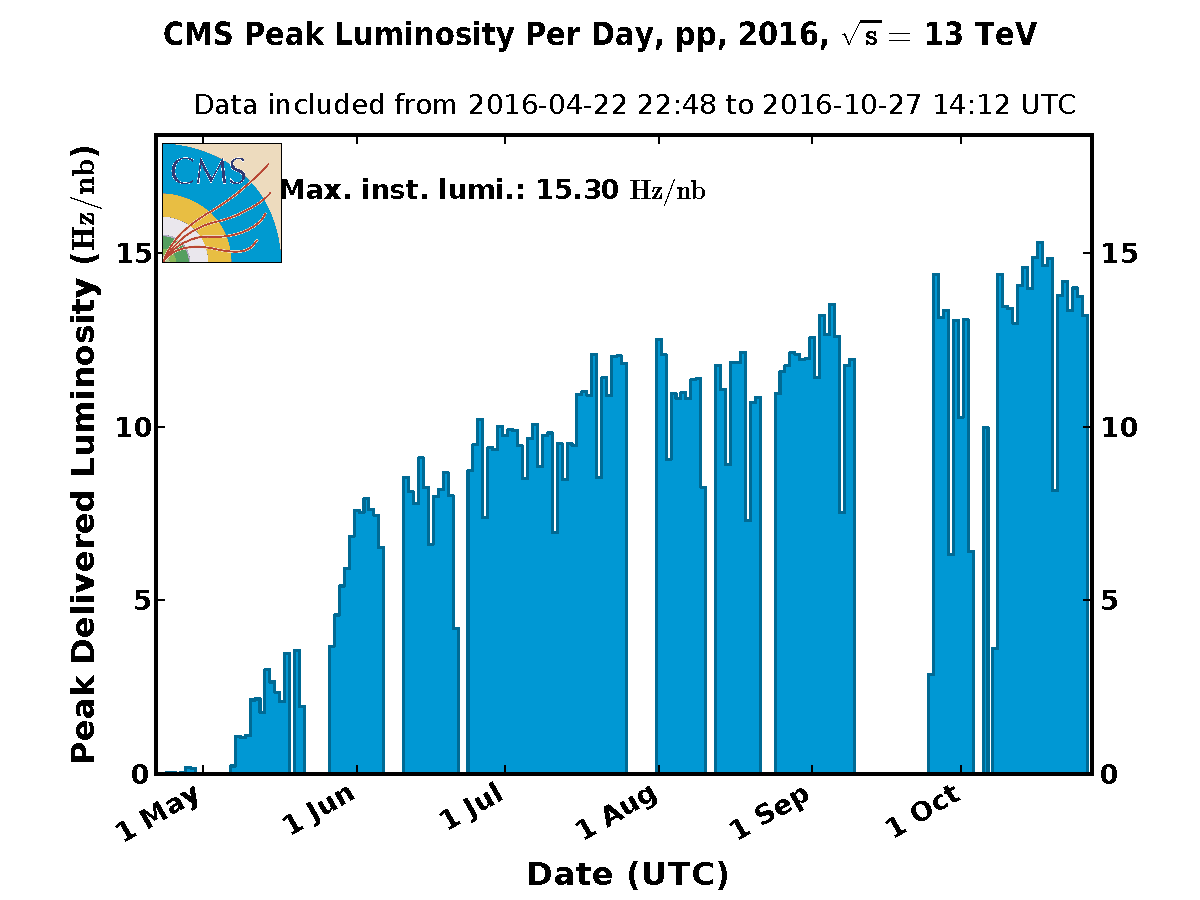
\includegraphics[width=.48\textwidth]{figures/peak_lumi_per_day_pp_2016.pdf}
    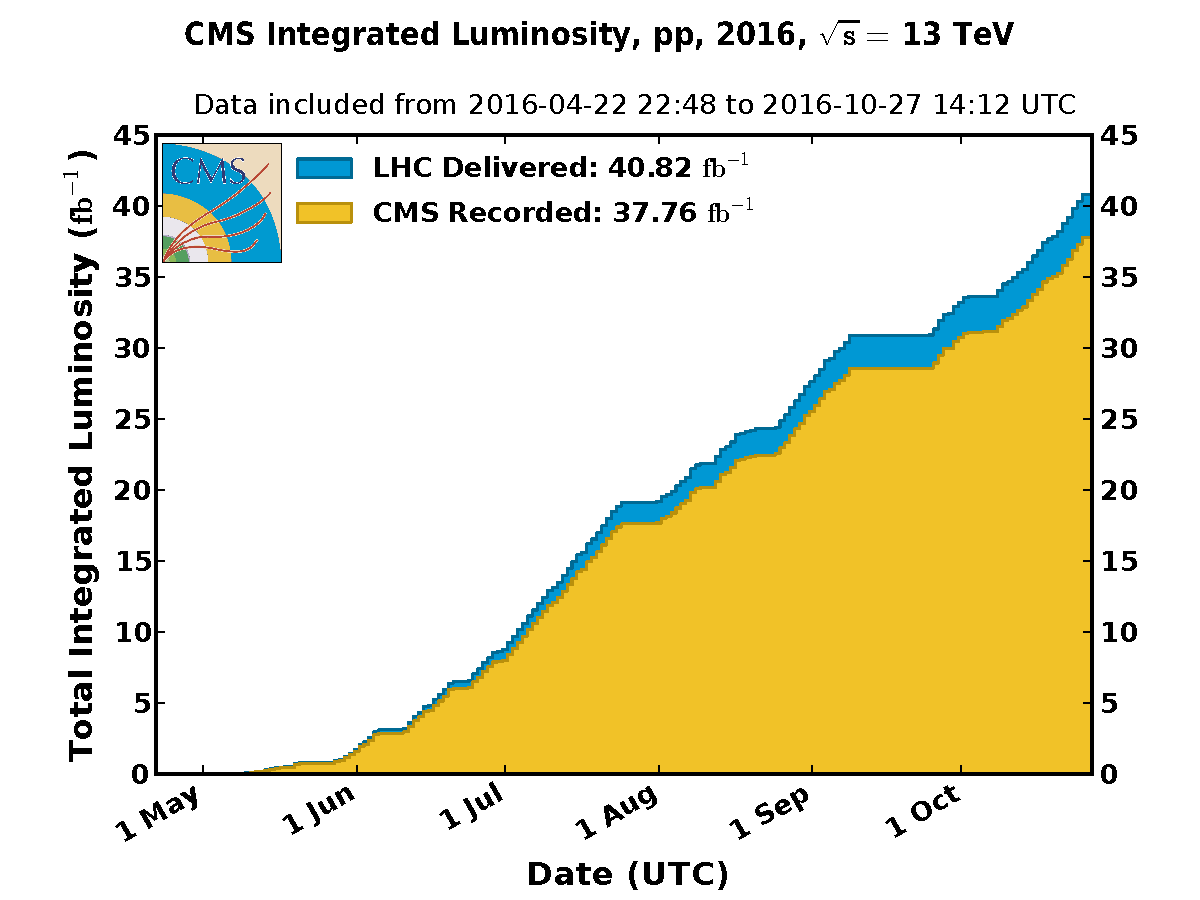
\includegraphics[width=.48\textwidth]{figures/int_lumi_per_day_cumulative_pp_2016.pdf}
    \caption{Peak instantaneous and integrated luminosity over time during the 2016 LHC proton-proton run delivered to the CMS detector. The difference between the 35.9 fb$^{-1}$ used in this analysis and the shown 37.76 fb$^{-1}$ comes from the omission of certain run periods where the detector was not operating optimally for the detection of leptons. Taken from \cite{lumi_twiki}.}
    \label{fig:lumi_stats}
  \end{figure}

  \subsection{What gets made?} \label{sec:what_gets_made}
    As mentioned in the previous section, the typical number of collisions leading to measurable energy deposits in the detector is 20 per bunch crossing. Figure \ref{fig:lhc_decay_modes} shows cross section for various proton-proton final states as a function of center of mass energy. Notice that the vast majority of the collisions result in low energy jet production or elastic scattering. 

    The analysis presented in this thesis is concerned with the production of Z bosons, whose production cross section is denoted as $\sigma_\text{Z}$ in the figure. Given the instantaneous luminosity of $10^{34}$ cm$^{-2}$ s$^{-1}$, the production cross section corresponds to a rate of 1000 Z bosons produced per second at peak luminosity. Given the total integrated luminosity of 35.9 fb$^{-1}$, the entire CMS dataset during this time period contained approximately 300 million Z bosons.

    Notice that the vast majority of collisions create only colored particles in the prompt process. Therefore, the most likely effect of the extra 20 collisions in a bunch crossing is to produce soft hadronic jets. For instance, the chance to produce another Z boson in an event that already has a Z boson is roughly 20 in a million, or 1 in 50,000. However, it is still important that particles from other collisions do not contaminate an event. As will be discussed more thoroughly in section \ref{sec:vertex_selection}, charged particle tracks can be traced back to the beamline and clustered into points of origin called a verticies. The vertex that is assigned the most total energy in an event is called the primary vertex. The chance that two high energy verticies will exist in a single event is low since the number of collisions per crossing is small compared the ratio of the cross section of interesting physics to the total proton-proton cross section.


    \begin{figure}[h!]
      \centering
      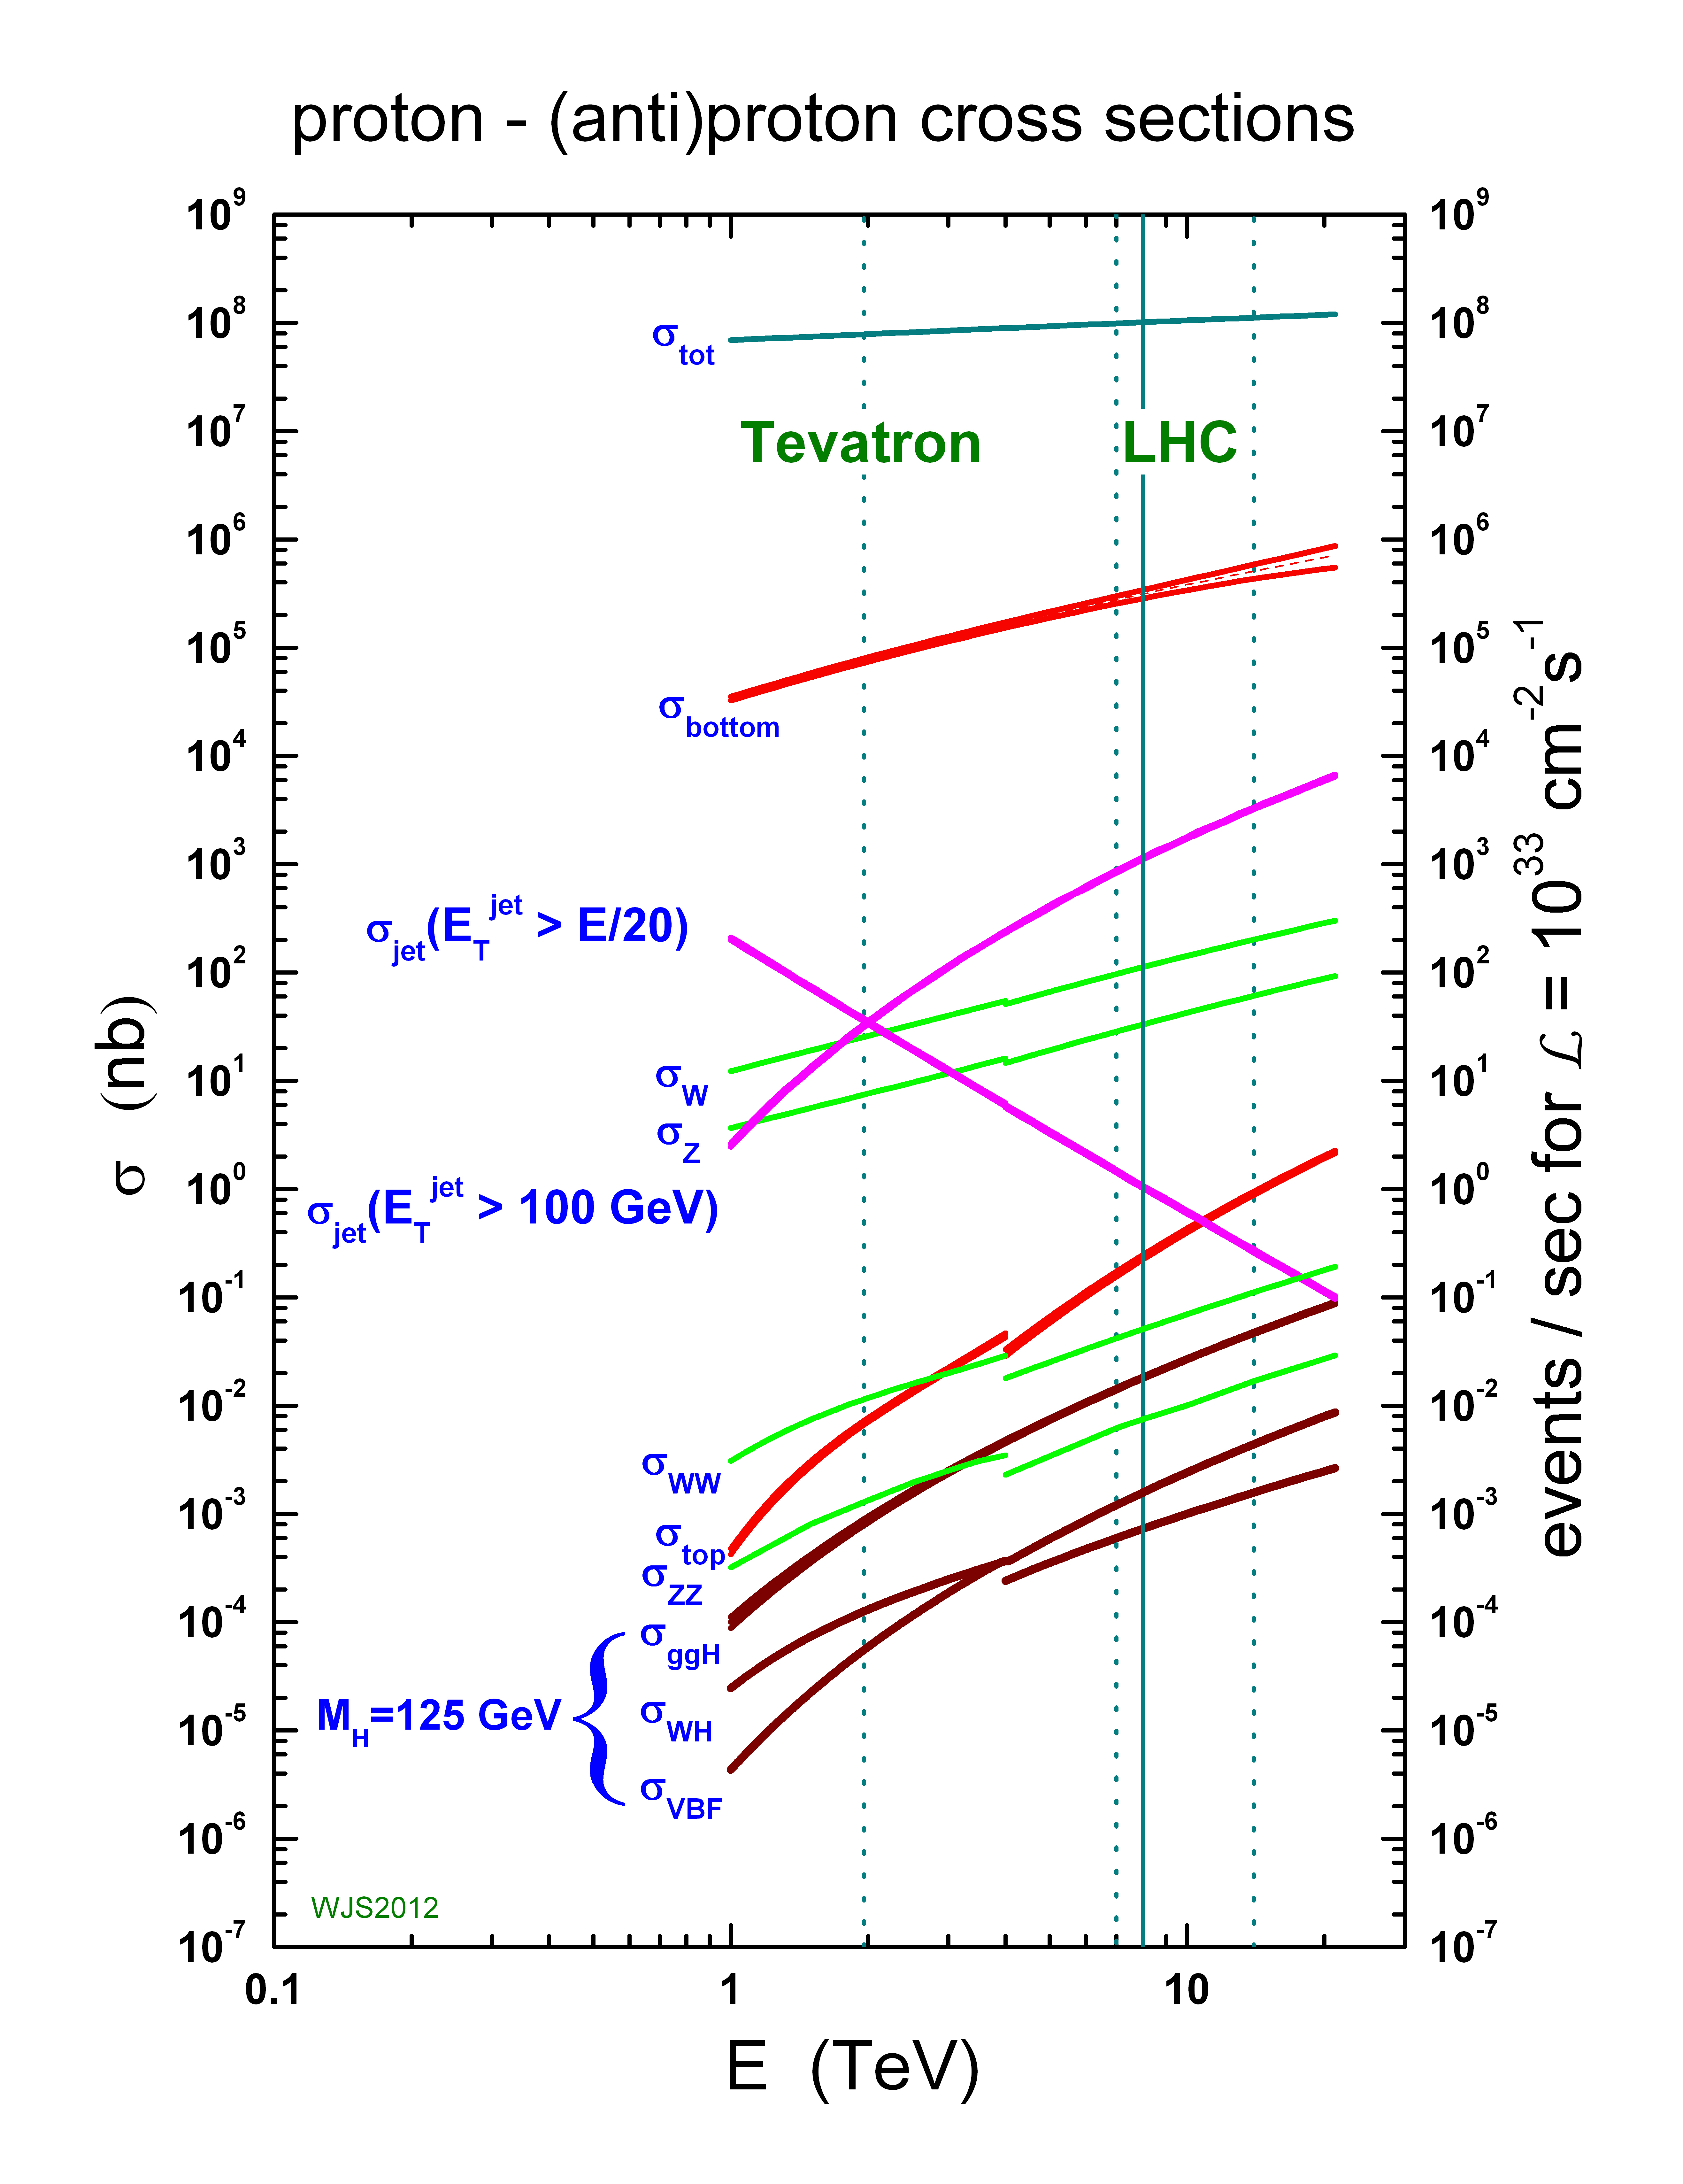
\includegraphics[width=.7\textwidth]{figures/lhc_decay_modes.jpg}
      \caption{Production Cross Sections for proton-proton collisions. Cross sections at center of mass energy less than 4 TeV are taken from proton-antiproton collision data at the Tevitron, which leads to some discontinuity for some types of electroweak boson production.}
      \label{fig:lhc_decay_modes}
    \end{figure}

    \begin{figure}[h!]
      \centering
      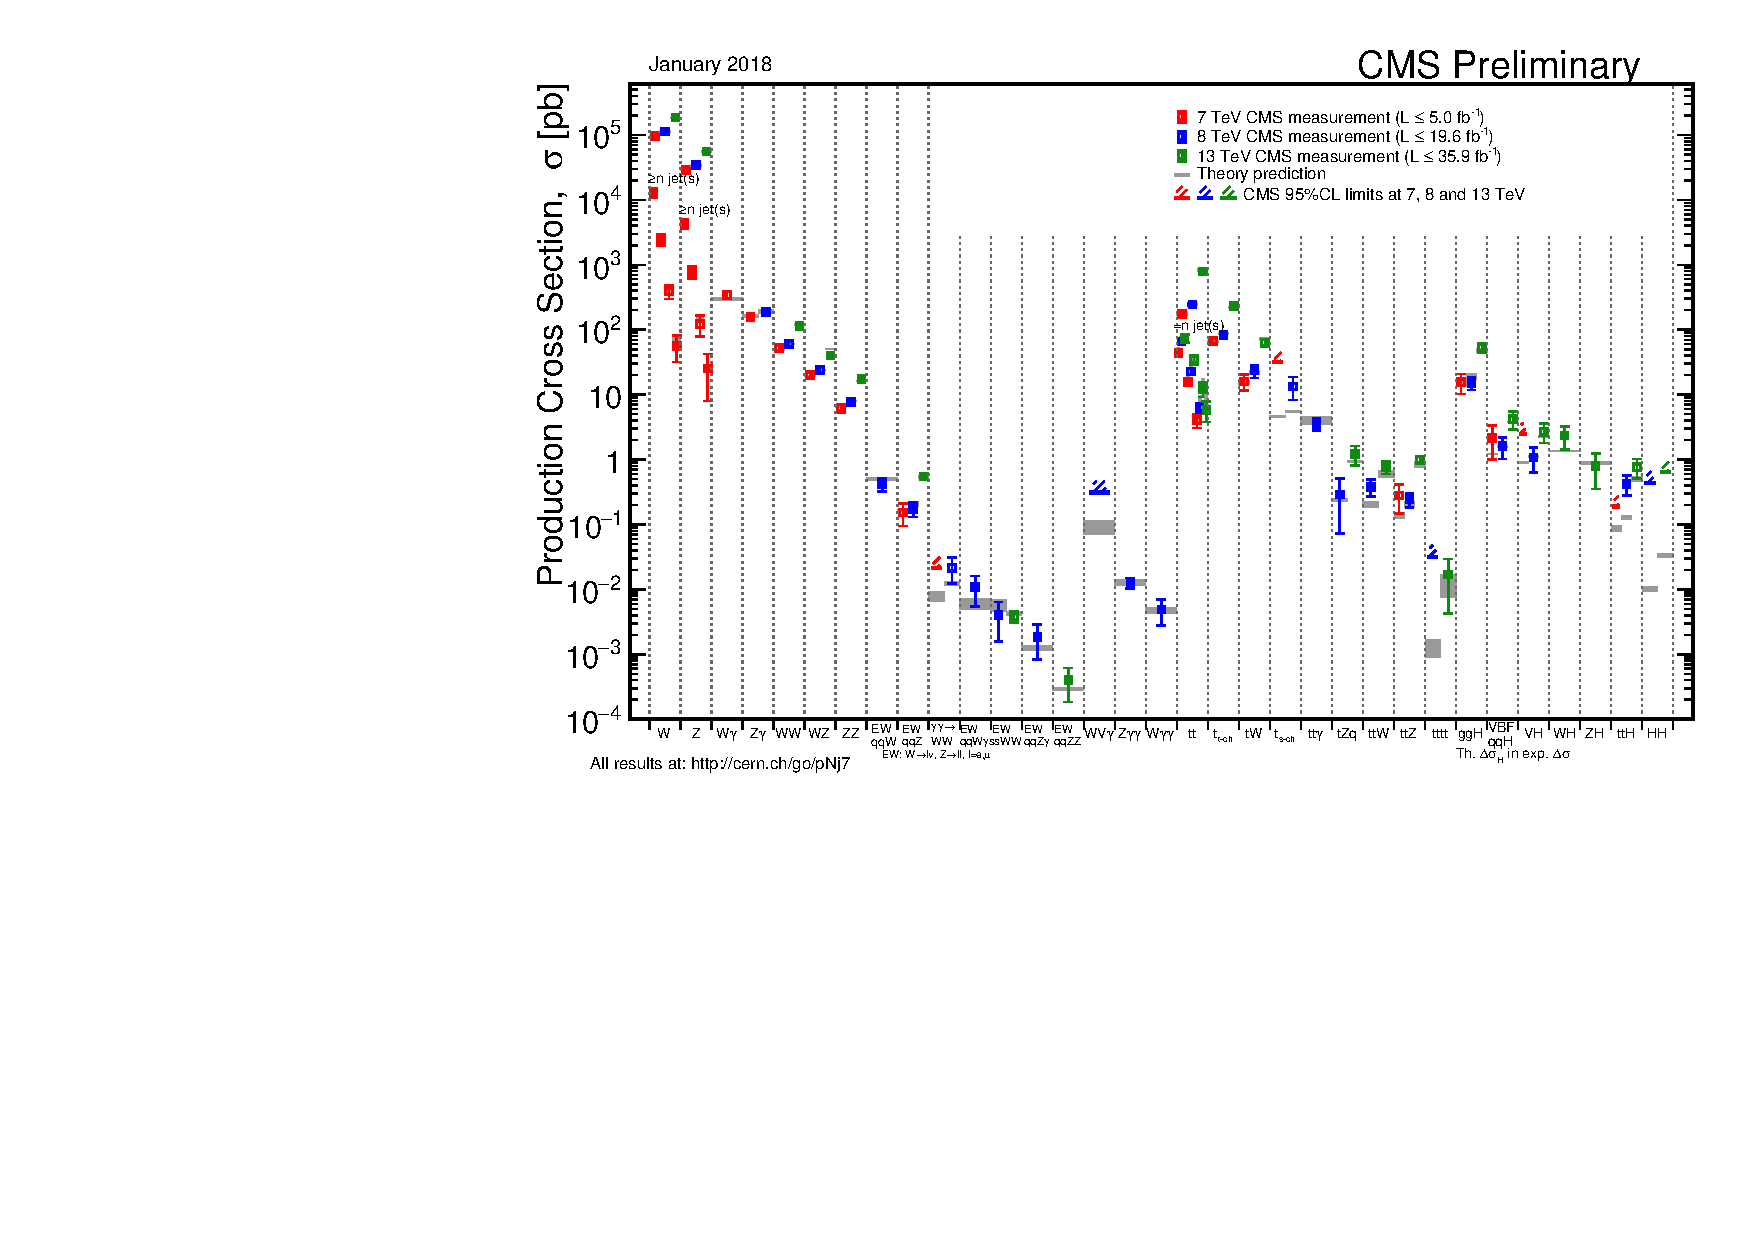
\includegraphics[width=.7\textwidth]{figures/cms_cross_sections.pdf}
      \caption{Cross sections measured by the CMS collaboration as of January 2018. Note that the cross section for Z+2 jets is close to the cross section for TTBar production. Additionally, note that for W and Z bosons, the cross section reduction in adding an additional jet is a factor between 5 and 10, consistent with the value of $\alpha_s$ at these energies. Taken from \cite{cms_results}}
      \label{fig:cms_cross_sections}
    \end{figure}

    \todo{Point out that there is very low chance for double scattering or two interesting interactions in one bunch crossing. 
    Point out cross section of Z boson, point out the NJets rule.
    Consider adding the other figure on my wall at the office. That way I can point out the njets rule and show the background composition with 2 jets.}

\section{The CMS Detector}
  
  The Compact Muon Solenoid (CMS) is a general purpose detector at the LHC. The detector is shown in figure \ref{fig:cms_detector}. It is the second largest detector at the LHC, weighing just under 15 kilotons. The envelope of the detector is a cylinder of radius 7.3 meters and length of 21.6 meters. The detector subsystems are embedded like an onion, sorted by what a particle produced at the interaction point would encounter traveling away from the beam pipe, the detector subsystems are as follows:

  \begin{enumerate}
    \item{Silicon Pixel Tracker}
    \item{Silicon Strip Tracker}
    \item{Electromegnetic Calorimeter}
    \item{Hadronic Calorimeter}
    \item{Superconducting Solenoid}
    \item{Muon Drift Tubes}
  \end{enumerate}

  The subsystems are broken into at least two regions. The \emph{barrel} region is the central part of the detector, and it is built of mostly of detection modules that are oriented parallel to the beam pipe, since particles traveling through this part of the detector have more transverse than longitudinal momentum. The \emph{end cap} contains modules oriented perpendicular to the beam pipe, since particles traveling through this part of the detector have more longitudinal momentum.

  \begin{figure}[h!]
    \centering
    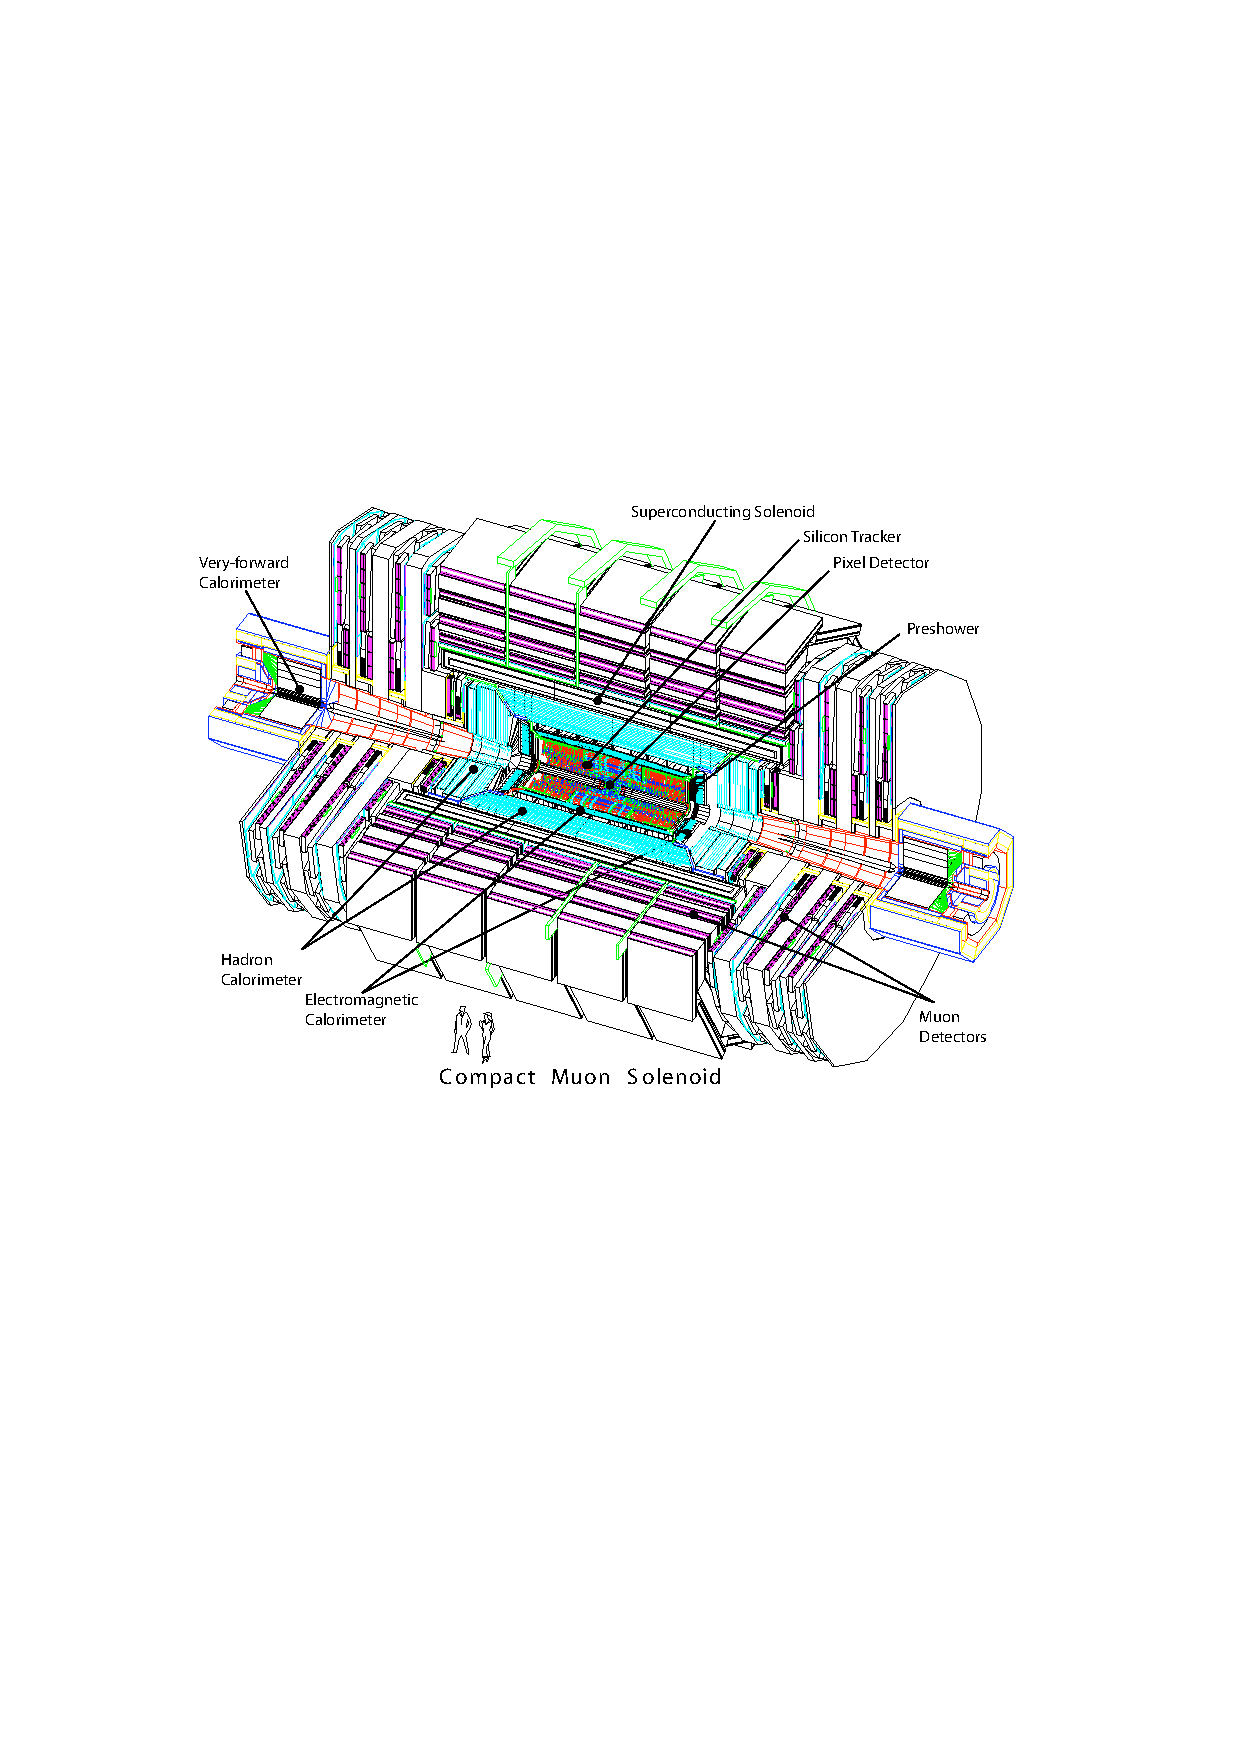
\includegraphics[width=.7\textwidth]{figures/cms_detector.pdf}
    \caption{A cutaway drawing of the Compact Muon Solenoid. Taken from the CMS TDR \cite{cms_tdr}.}
    \label{fig:cms_detector}
  \end{figure}

  As was shown in sec \ref{sec:what_gets_made}, most collisions at the LHC produce sprays of hadrons called jets, in fact the bulk of interactions are between gluons. However, more rare electroweak processes, such as the production of the higgs boson, can lead to the creation of leptons. Therefore, measuring the energy spectra of leptons is of central importance for CMS analyses searching for new physics coupled to the electroweak sector; this search is one such analysis. 

  The CMS detector needs to be able to identify charged leptons and distinguish their flavor in order to probe electroweak physics without hadronic backgrounds. The electron is a stable particle, and the muon has a lifetime long enough that it should make it through

  In order to measure the momentum of charged particles, a large magnetic field is applied by a superconducting solenoid that is placed between the hadronic calorimeter and the muon system. The solenoid creates a roughly constant 3.8 Tesla magnetic field parallel to the beam pipe in the region of the detector filled by the tracking system and calorimeters. This magnetic field will bend charged particles in accordance with the Lorentz force law and allow for a measurement of the particles momentum.

  CMS was designed with several physics goals in mind, from finding the Higgs boson, to searches for dark matter and supersymmetry. The technical design report (TDR) \cite{cms_tdr} summarizes the physics and design goals for the detector. A short list follows:

  \begin{enumerate}
    \item The search for the Higgs boson, specifically in the dimuon and diphoton channel\footnote{the diphoton channel was where it ultimately was found}. This created a need for excellent muon and photon energy resolution and isolation. These requirements justify the advanced muon system and ECAL. Additionally searching for the Higgs in the $b\bar{b}$ and $\tau \bar{\tau}$ channels created the requirement for good offline b-tagging and $\tau$-tagging capabilities, largely regulated by tracker resolution.
    \item The search for supersymmetric (SUSY) particles. The main motivation for these searches is often in the context of R-parity conserving SUSY due to the natural dark matter candidate they provide as described in section \ref{sec:r-parity}. Dark particles leave momentum imbalance in the detector, so there is 
    \item The search for new massive vector bosons, typically dubbed a Z' search. Here dilepton (electron and muon) energy resolution are again of the paramount importance.
    \item The search for extra dimensions. The phenomenology of these models is very broad, but signatures can include all massive standard model particles and gravitons which leave a \MET signature.
    \item Measurements furthering the precision Standard Model parameters. The production of top quarks is enhanced at the LHC compared to any previous colliders due to their large mass, even compared to the TeV scale. Top quarks almost always decay to b-quarks which means the LHC is also a b-factory.
    \item In addition to proton-proton collisions, the LHC also collides lead ions which probe the thermodynamic properties of quantum chromodynamics (QCD), the theory of the strong nuclear force. These collisions typically produce hadronic jets and their \pt spectrum is of interest due to observations at RHIC \cite{QCD_collider_physics}.
  \end{enumerate}

  \subsection{Coordinate System}
    Throughout this document, a standard coordinate system is used, this system is a cylindrical coordinate system with the $z$ axis oriented along the beam pipe. $z=0$ is situated at the mid-point of the detector, 10.8 m from either edge. The $\theta = 0$ direction points toward the Jura mountains, with $\theta = 90^\circ$ pointing straight upwards, away from the center of the earth. 

    Rather than $\theta$, we use the pseudorapidity, $\eta = - \ln \left( \tan\left(\frac{\theta}{2}\right)\right)$. $\eta = 0$ corresponds to $\theta = 90^\circ$ and $\eta$ grows to infinity as $\theta$ goes to 0. The benefit of using $\eta$ is that differences in $\eta$, $\Delta \eta$, between two particles are approximately invariant under Lorentz boosts along the beam axis, whereas differences in $\theta$ are not. The extent to which $\Delta \eta$ is equal in different reference frames is regulated by the mass of the particles, with equality achieved in the case where the mass to momentum ratio of the particles goes to 0, i.e. the high energy limit.\footnote{Pages 6-8 in reference \cite{psuedorapidity} shows that differences in rapidity are Lorentz invariant and that psuedorapidity and rapidity are equal in the high energy limit} The detector's fiducial area corresponds to about $\abs{\eta} < 2.4$, which is about $10^\circ$ off of the beampipe. The positive $x$ axis is defined as pointing to the center of the circle outlined by the LHC, and the positive $y$ axis points towards the sky. The $\phi$ direction is the angle from the positive $x$ axis to the positive $y$ axis. Figure \ref{fig:cms_coordinates} shows this information visually.

    \begin{figure}[h!]
      \centering
      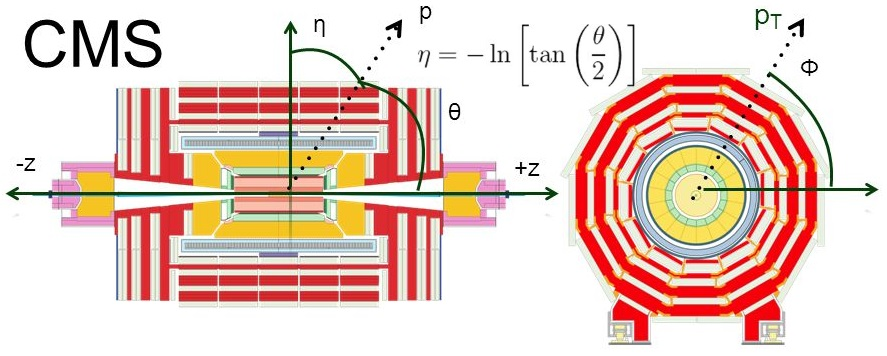
\includegraphics[width=.7\textwidth]{figures/cms_coordinates.jpg}
      \caption{Cross sectional and transverse views of the CMS detector with $\eta$, $\phi$, and $\theta$ coordinates shown. Taken from \cite{cms_coordinates}.}
      \label{fig:cms_coordinates}
    \end{figure}

  \subsection{The Inner Tracker} \label{sec:inner_tracker}
    The inner tracker is the closest part of the CMS detector to LHC beamline and interaction point where protons collide. \cite{cms_jinst} It surrounds the interaction point with a length of 5.8m and radius of 1.25m. The purpose of the system is to track charged particles to their vertex and measure the momentum of charged particles via the saggita in the particle arc due to the magnetic field. The entire active detection area of the inner-tracker system is made of silicon, but can be broken into 2 main subsystems:

    \begin{enumerate}
      \bitem{pixel detectors} The innermost part of the tracker system is a pixel-based detector composed of 1,440 thin modules, of cross section $100 \times 150 \mu$m$^2$, capable of measuring hits with fine granularity in 3 dimensions. This subsystem's main purpose is to aid in vertex reconstruction.
      \bitem{strip detectors} The outer part of the inner tracker is composed of 15,148 strip modules. The main purpose of this subsystem is to track charged particles from the vertex into the ECAL and also to give one measure of their momentum.
    \end{enumerate}

    Silicon detectors work on the principle of semi-conduction. When a charged particle passes through the material, electrons are kicked into the conduction band and drift, due to a bias voltage applied across the sample, towards electronics attached to the material that record the current. Because silicon has a relatively small band gap, the entire tracking system needs to be kept at low temperature, approximately $-10^\circ$ C, in order to keep the electrons stationary in the valence band in the presence of the bias voltage.

    The tracker geometry is shown in figure \ref{fig:strip_tracker_geometry}. The pixel detectors are the closest to the beampipe and consist of 3 layers in the barrel region and 2 annuli in the endcap region. The three barrel layers are positioned in concentric cylinders about the beampipe at radii of 4.4 cm, 7.3 cm, and 10.2 cm respectively. The endcap annuli are placed at $\abs{z} = 34.5 $cm and 46.5 cm respectively and have an inner radius of 6 cm and an outer radius of 15 cm. The strip tracker consists of an inner barrel region (TIB), an outer barrel region (TOB), and an inner disk region (TID) in the barrel, and two endcap regions (TEC +/-). 

    \begin{figure}[h!]
      \centering
      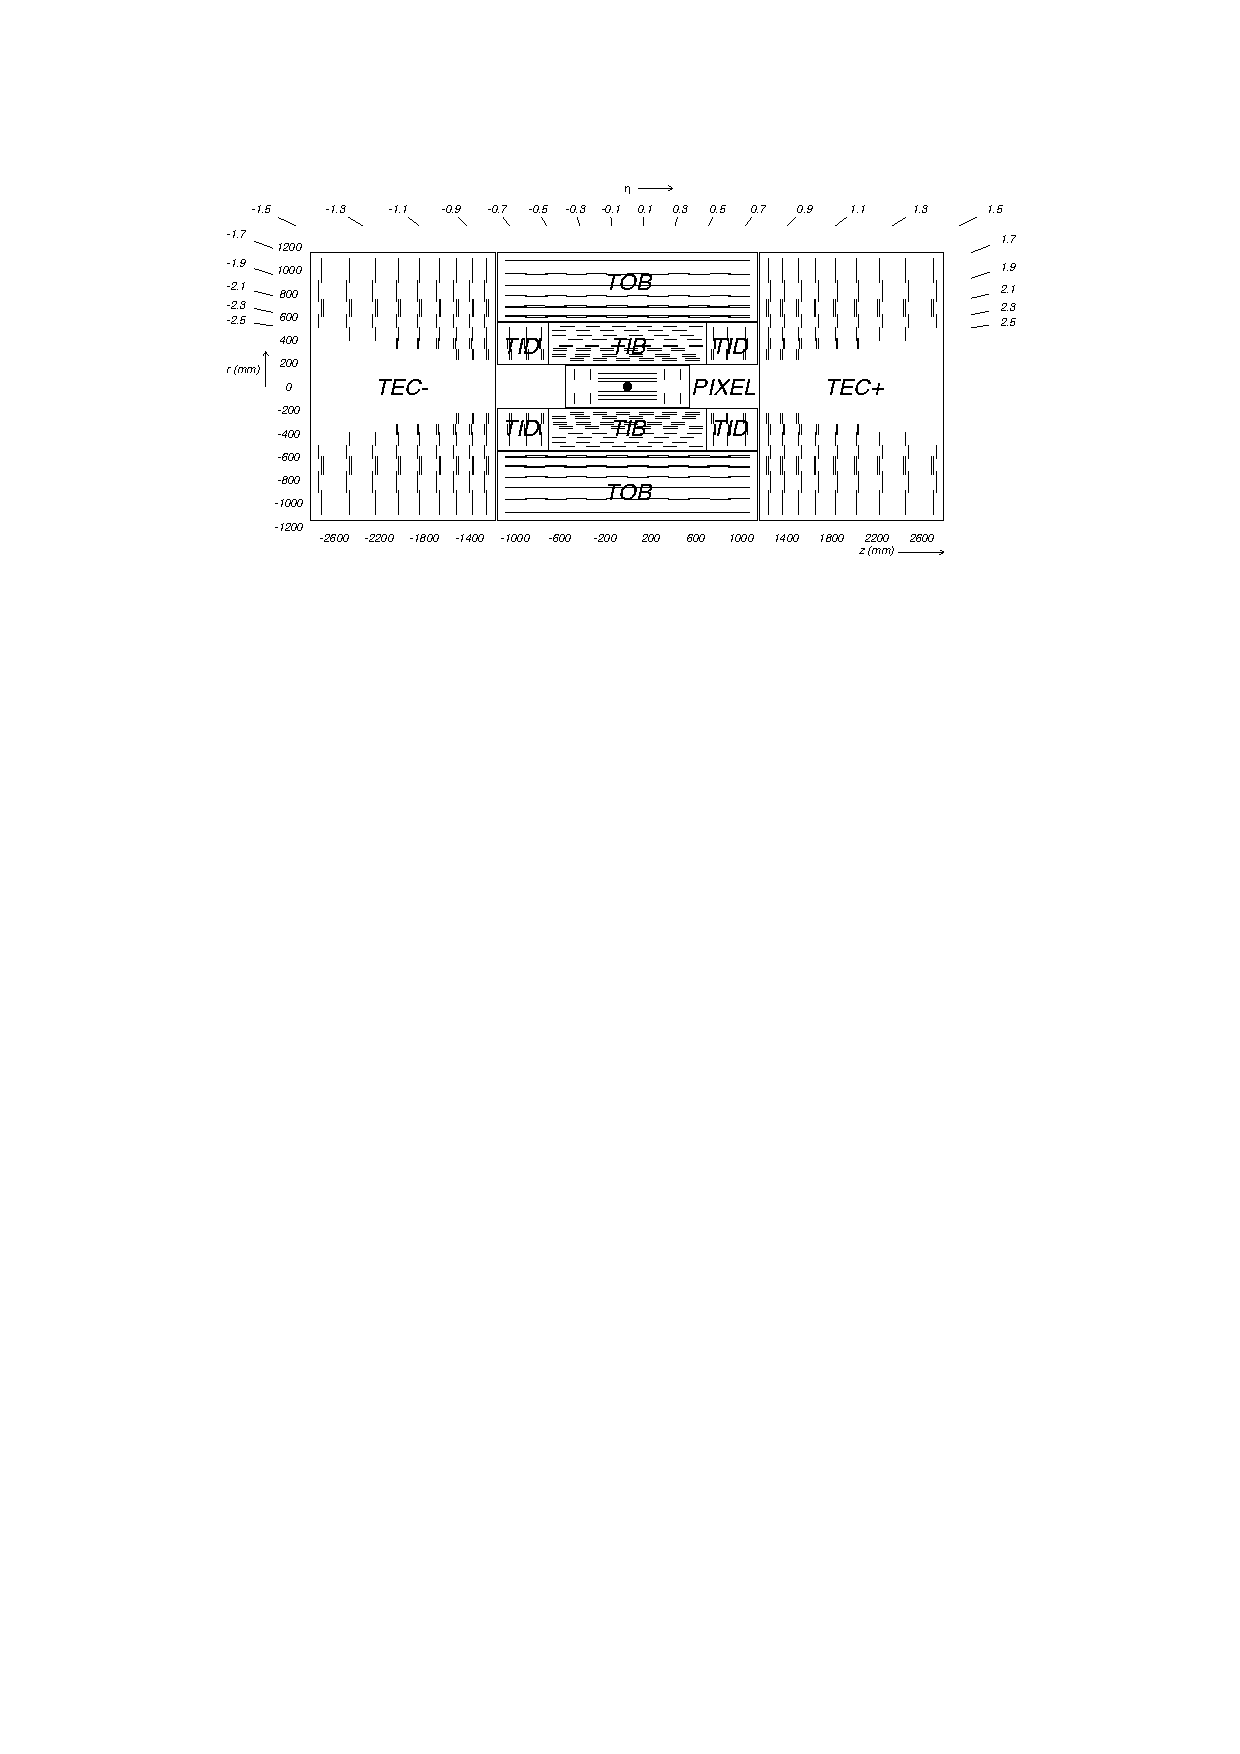
\includegraphics[width=.7\textwidth]{figures/cms_tracker_schematic.pdf}
      \caption{Schematic view of the CMS inner tracking system. Notice the detectors only cover $\abs{\eta}$ ranges less than 2.5 and that particles traveling near $\abs{\eta}=1.5$ pass through the most material. Taken from \cite{cms_jinst}.}
      \label{fig:strip_tracker_geometry}
    \end{figure}

    Because one of the goals of the tracking system is to obtain a measure of momentum by tracking the natural motion of particles through space in a magnetic field, it is important that the interactions between charged particles and the tracking system do not change the motion, and likewise the energy, of the particles dramatically. For particles other than the electron and photon, the silicon tracker has mostly negligible effects on the energy as the amount of bremsstrahlung is inversely proportional to the mass of the particle to approximately the 6th power;\footnote{This can be seen in the classical theory of bremsstrahlung radiation as described in \cite[pg. 464, eq. 11.75]{griffiths_em} by replacing the Lorentz factor $\gamma$ with $\frac{E}{mc^2}$. In the case of an acceleration in an orthogonal direction, $\gamma^6 \to \gamma^4$.} their main energy loss mechanism is through ionization.\cite[sec. 33.2]{PDG} However, for the electron and the photon, interaction with the tracker can cause bremsstrahlung radiation and pair production respectively.

    To understand the magnitude of these effects, it is typical to look at the number of radiation lengths\footnote{taken to be the distance at which a high energy electron is expected to lose $\frac{1}{e}$ of its energy \cite[sec 34.4.2]{PDG}, or $\frac{7}{9}$ the mean free path for a high energy photon.} of material in the tracker. The ``material budget" of the tracker is shown in figure \ref{fig:tracker_material_budget}. Due to the large amount of non-sensitive material in the range $\abs{\eta} \in [1.4,1.6]$, leptons for this analysis are not considered in that range, as is explained in section \ref{sec:dilepton_selection}. As can be seen in the figure, many $\eta$ values correspond to high probability of radiation and pair production for electrons and photons respectively. We will explain in section \ref{sec:particle_flow} how the momentum of these types of particles is reconstructed given these issues.

    \begin{figure}[h!]
      \centering
      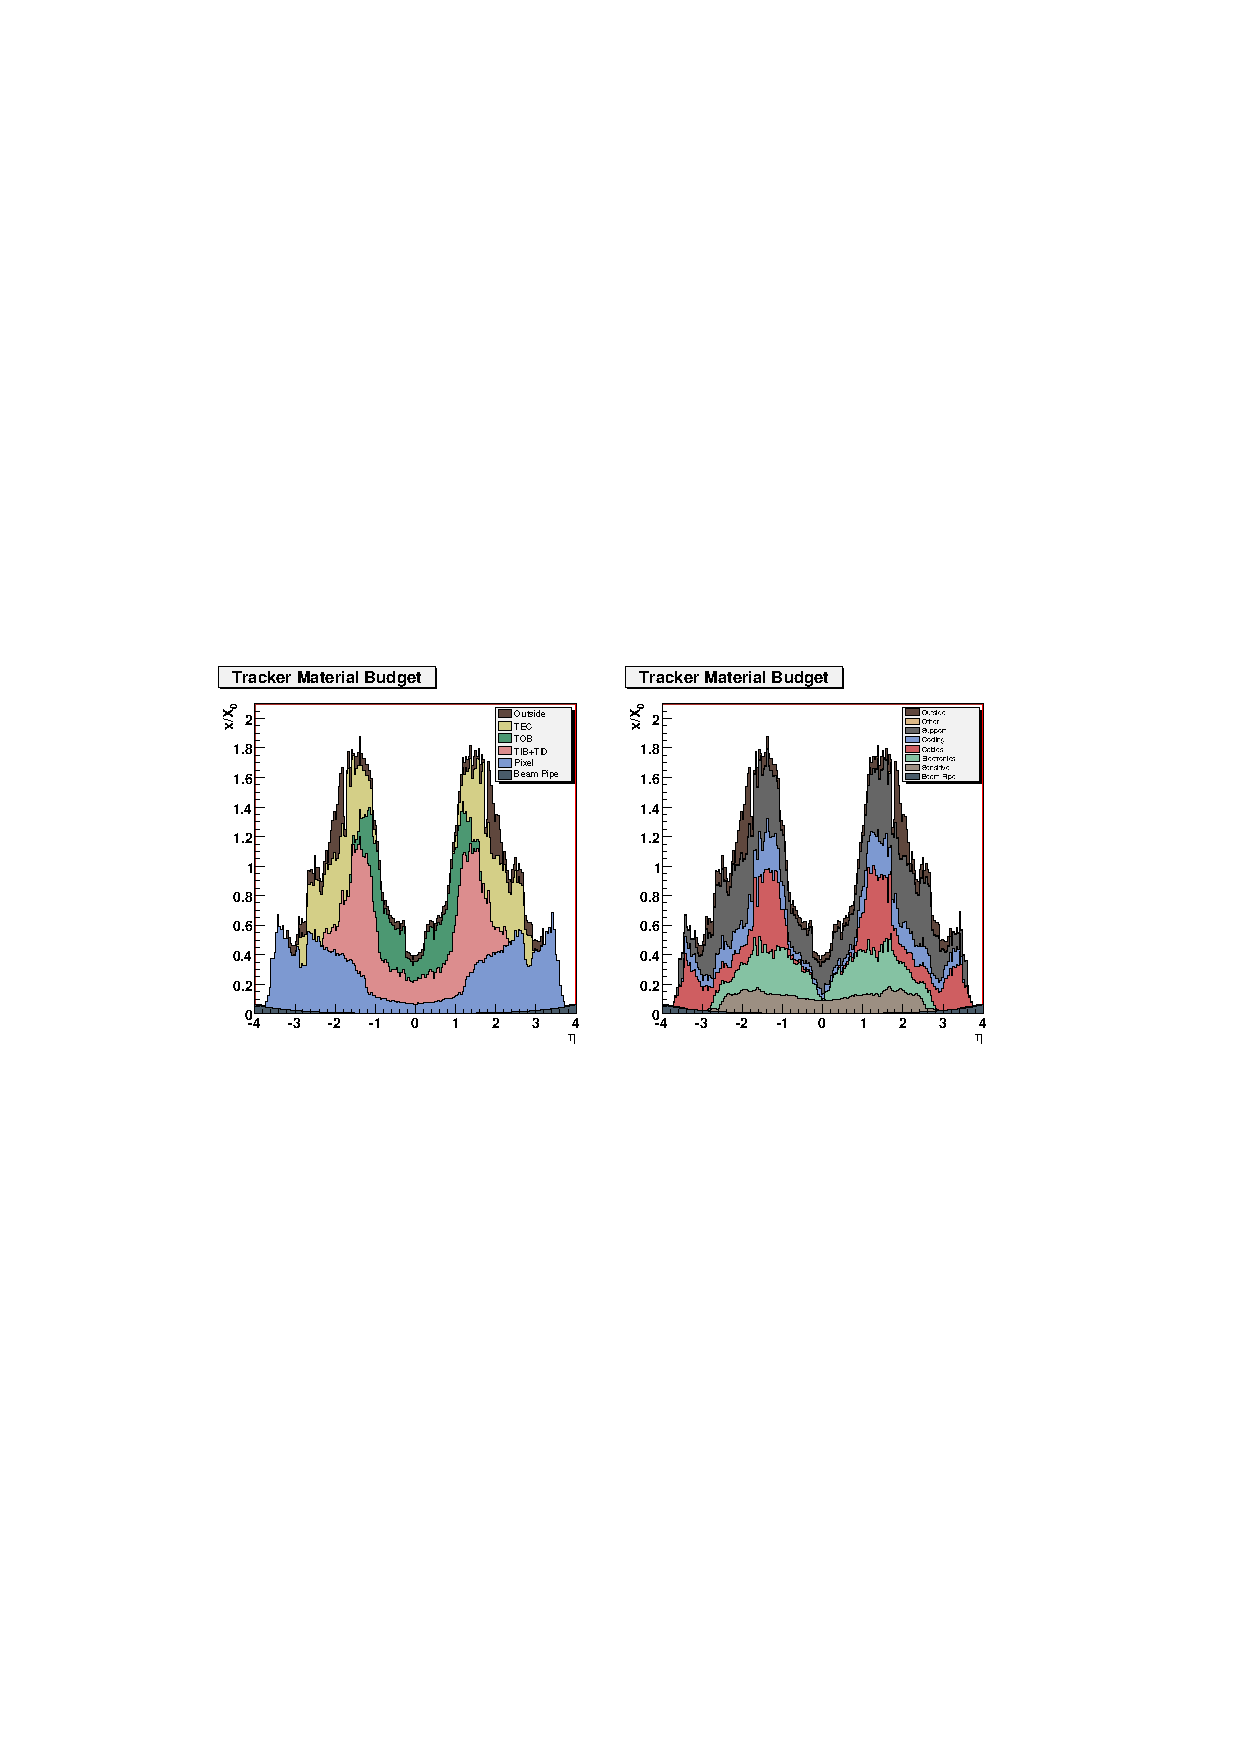
\includegraphics[width=.9\textwidth]{figures/cms_tracker_material_budget.pdf}
      \caption{The material budget of the tracking system in radiation lengths. On the left, the material is broken down by tracker subsystem, on the right it is broken down by the type of component. As can be seen on the right plot, a large amount in non-sensitive material, like cables and support structure, is found near $\abs{\eta}=1.5$. For this reason, leptons in this analysis are not used if they are found in the window $\abs{\eta} \in [1.4,1.6]$. Taken from \cite{cms_jinst}.}
      \label{fig:tracker_material_budget}
    \end{figure}

  \subsection{The Electromagnetic Calorimeter} \label{sec:ECAL}
    The CMS Electromagentic Calorimeter (ECAL) is a nearly hermetic and homogeneous cylinder made of lead tungstate (PbWO$_4$) crystals with attached light measuring devices. The crystals are ``truncated pyramids", roughly rectangles of approximately 23 centimeters in length that taper slightly, from 26x26 mm$^2$ to 22x22 mm$^2$ in the barrel\cite[pg. 4]{cms_ecal}, to accommodate the curved shape of the ECAL in the $\phi$ direction and the angle at which the crystals are oriented to face the interaction point.\footnote{the crystals have a 3$^\circ$ angle with respect to the line that connects their incident face to interaction point in both the $\eta$ and $\phi$ directions to allow for better coverage of the fiducial volume.} Schematic views of the ECAL can be seen in figures \ref{fig:ecal_xsec} and \ref{fig:ecal_cutaway}. As can be seen in the figures, the calorimeter is broken into two physical sections, the barrel region (EB) and the endcap region (EE). The preshower disk in front of the endcap region is immaterial for this search, but is there to help distinguish between neutral pions converting to a di-photon pair with small angle separation from a single high energy photon. 

    \begin{figure}[h!]
      \centering
      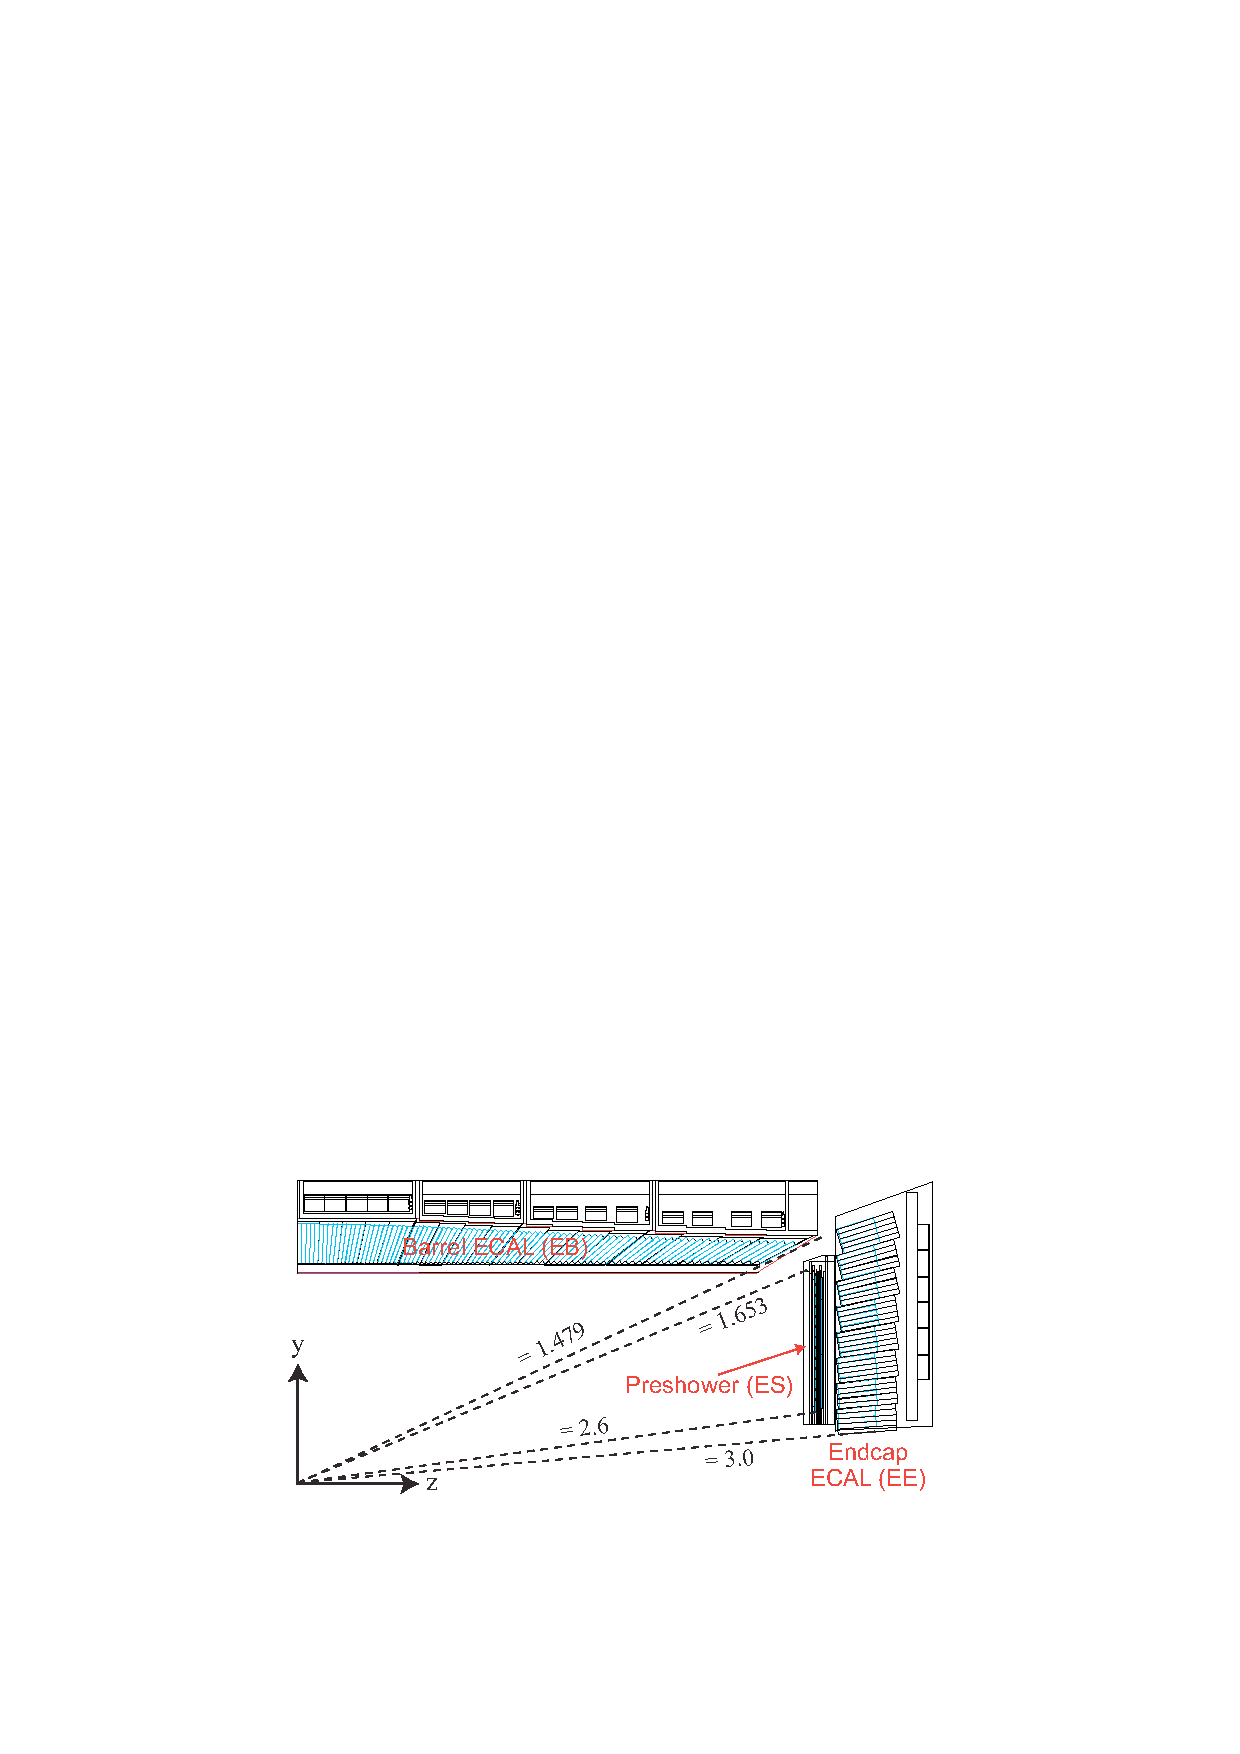
\includegraphics[width=.9\textwidth]{figures/cms_ecal_xsec.pdf}
      \caption{A cross sectional view of the electromagnetic calorimeter on the CMS detector. Notice the geometry of the crystals the transition region near $\abs{\eta} = 1.5$. Taken from \cite{cms_tdr}.}
      \label{fig:ecal_xsec}
    \end{figure}

    \begin{figure}[h!]
      \centering
      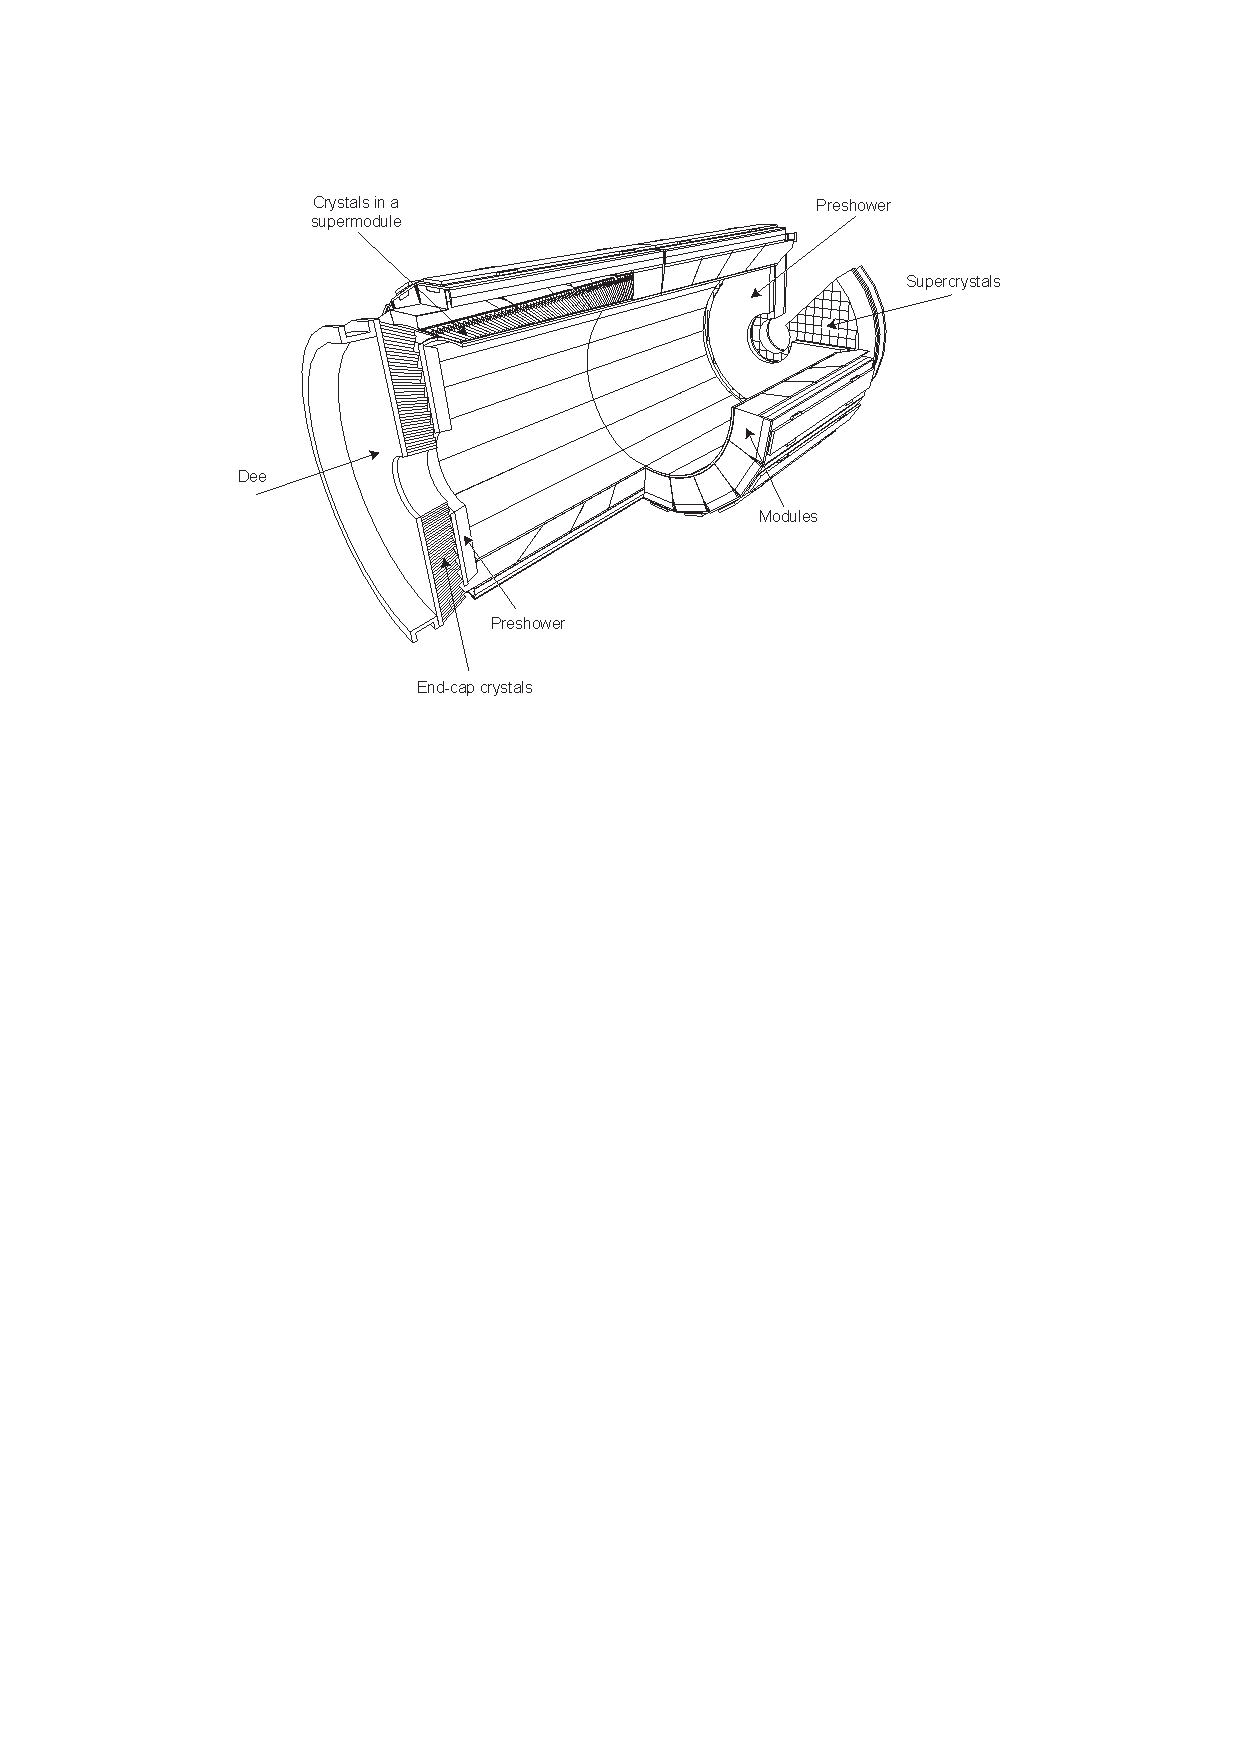
\includegraphics[width=.9\textwidth]{figures/cms_ecal.pdf}
      \caption{A cutaway of the electromagnetic calorimeter on the CMS detector. Taken from \cite{cms_jinst}.}
      \label{fig:ecal_cutaway}
    \end{figure}

    The purpose of the ECAL is essentially to give the most important measure of energy for electrons and photons. As explained in the previous section, the dynamics of electrons in material are quite distinct from heavier charged particles in material, the next lightest being a muon. Typical muon deposits in the ECAL are roughly 300 MeV\cite{muon_stopping_power}, whereas electrons under 500 GeV tend to have almost all of their energy absorbed by the ECAL\cite[sec. 4.10]{cms_jinst}. This is to say that charged particles heavier than an electron tend to pass right through the ECAL with little disturbance. \todo{Is this actually correct? Should I have a section somewhere where I describe charged particle interactions with matter?}

    The ECAL operates on the principle of scintillation\cite[ch. 7]{leo_detectors}, and makes use of the fast scintillation time (80\% of light emitted within 25 ns), high stopping power, and consequently small Moli\`ere radius of lead tungstate. The lead tungstate crystals have a length which corresponds to approximately 25 radiation lengths, this ensures that almost all of the energy carried by a high energy photon or electron will be radiated. The small Moli\`ere radius allows for good spacial resolution of energy deposits. \cite[pg. 90]{cms_jinst} Two things happen when an electron or photon is incident on one of the crystals:

    \begin{enumerate}
      \item A cascade of electrons, positrons, and photons is created. This is due to the effects discussed in the previous section, photons will pair produce electron-positron pairs. Electrons and positrons undergo bremsstrahlung radiation in material creating high energy photons. The result is that these processes feedback on each other and the multiplicity of particles explodes in the material creating an ``electromagnetic shower". A hypothetical shower imposed on an ECAL crystal is shown in figure \ref{fig:ecal_crystal}.

      \item Scintillation light is emitted by the lead tungstate due to interactions with charged particles and the light captured by the photo detectors attached to the crystal.
    \end{enumerate}

    \begin{figure}[h!]
      \centering
      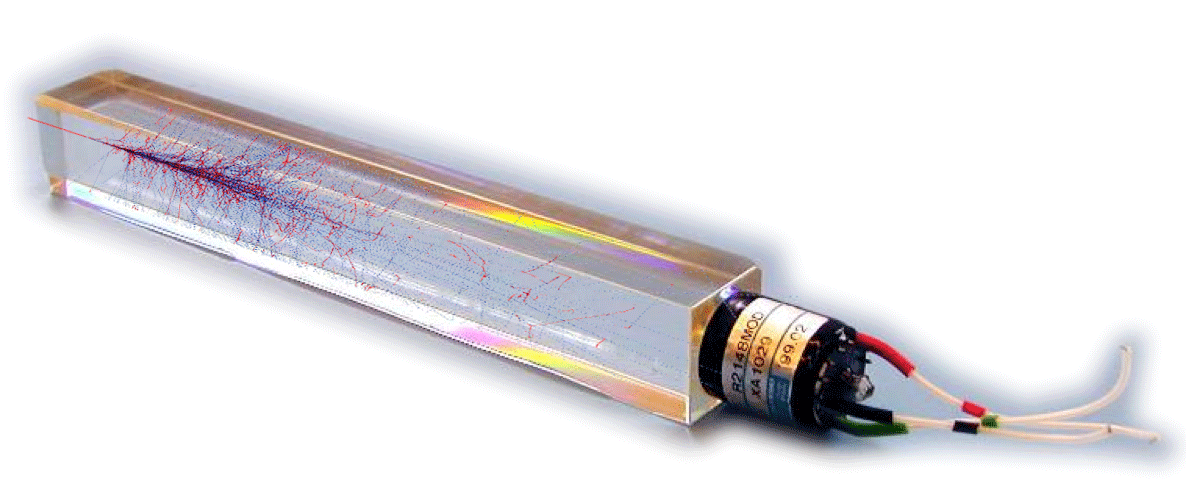
\includegraphics[width=.5\textwidth]{figures/cms_ecal_crystal_shower.png}
      \caption{A lead tungstate crystal from the CMS ECAL endcap region with a vacuum phototriode attached. A hypothetical shower from an electron is superimposed on the image. Taken from \cite{ecal_crystal}.}
      \label{fig:ecal_crystal}
    \end{figure}

    From the amount of scintillation light, the energy of the incident particle can be reconstructed with high resolution. Figure \ref{fig:ecal_resolution} shows the energy measured using a 5x5 grid of ECAL crystals for 120 GeV electrons. From the figure, we can see that the ECAL energy resolution is excellent for electrons in this range, the standard deviation of the energy measurement being 1-2\% of the energy.

    \begin{figure}[h!]
      \centering
      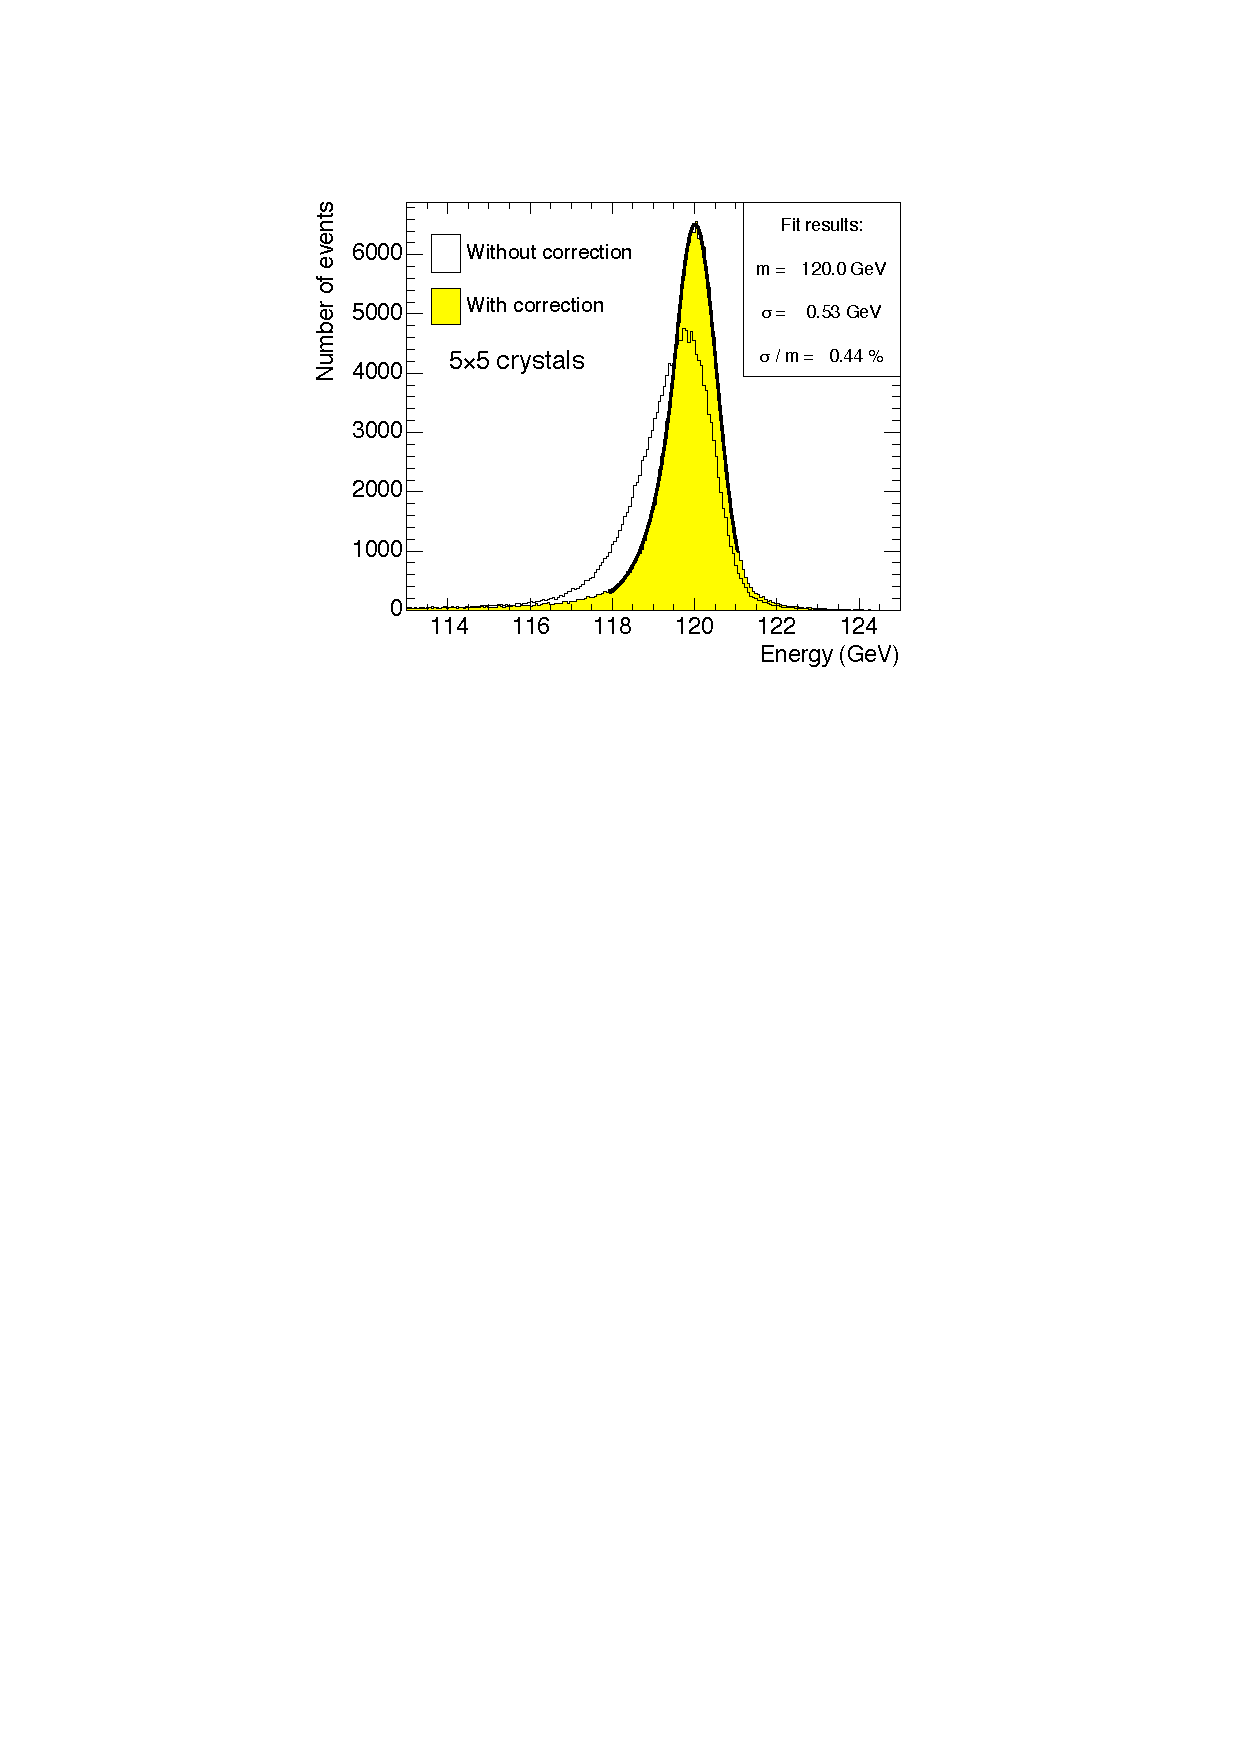
\includegraphics[width=.7\textwidth]{figures/ecal_resolution.pdf}
      \caption{The energy measured from 120 GeV electrons taken from a 5x5 grid of ECAL crystals. Taken from \cite{cms_jinst}.}
      \label{fig:ecal_resolution}
    \end{figure}

    \todo{What happens to the light that that doesn't pair produce? Is that also picked up by the photo diode? Also, why does the light always go forward, momentum only?}
    \todo{If I have time, I should throw in some stuff about the ECAL energy resolution. Specifically how the ECAL crystals are calibrated from \cite{ecal_energy_reco} and \cite[pg.20]{Electron_reco} }

  \subsection{The Hadronic Calorimeter}
    The CMS Hadronic Calorimeter (HCAL) is a sampling calorimeter made of interleaved layers of dense absorber metals with plastic scintillator material. The purpose of this subsystem is to measure the energy of the hadrons and massive charged particles that make up jets. The measurement of these objects are of particular importance for the reconstruction of \MET, which is a central event-level object in this analysis.

    \begin{figure}[h!]
      \centering
      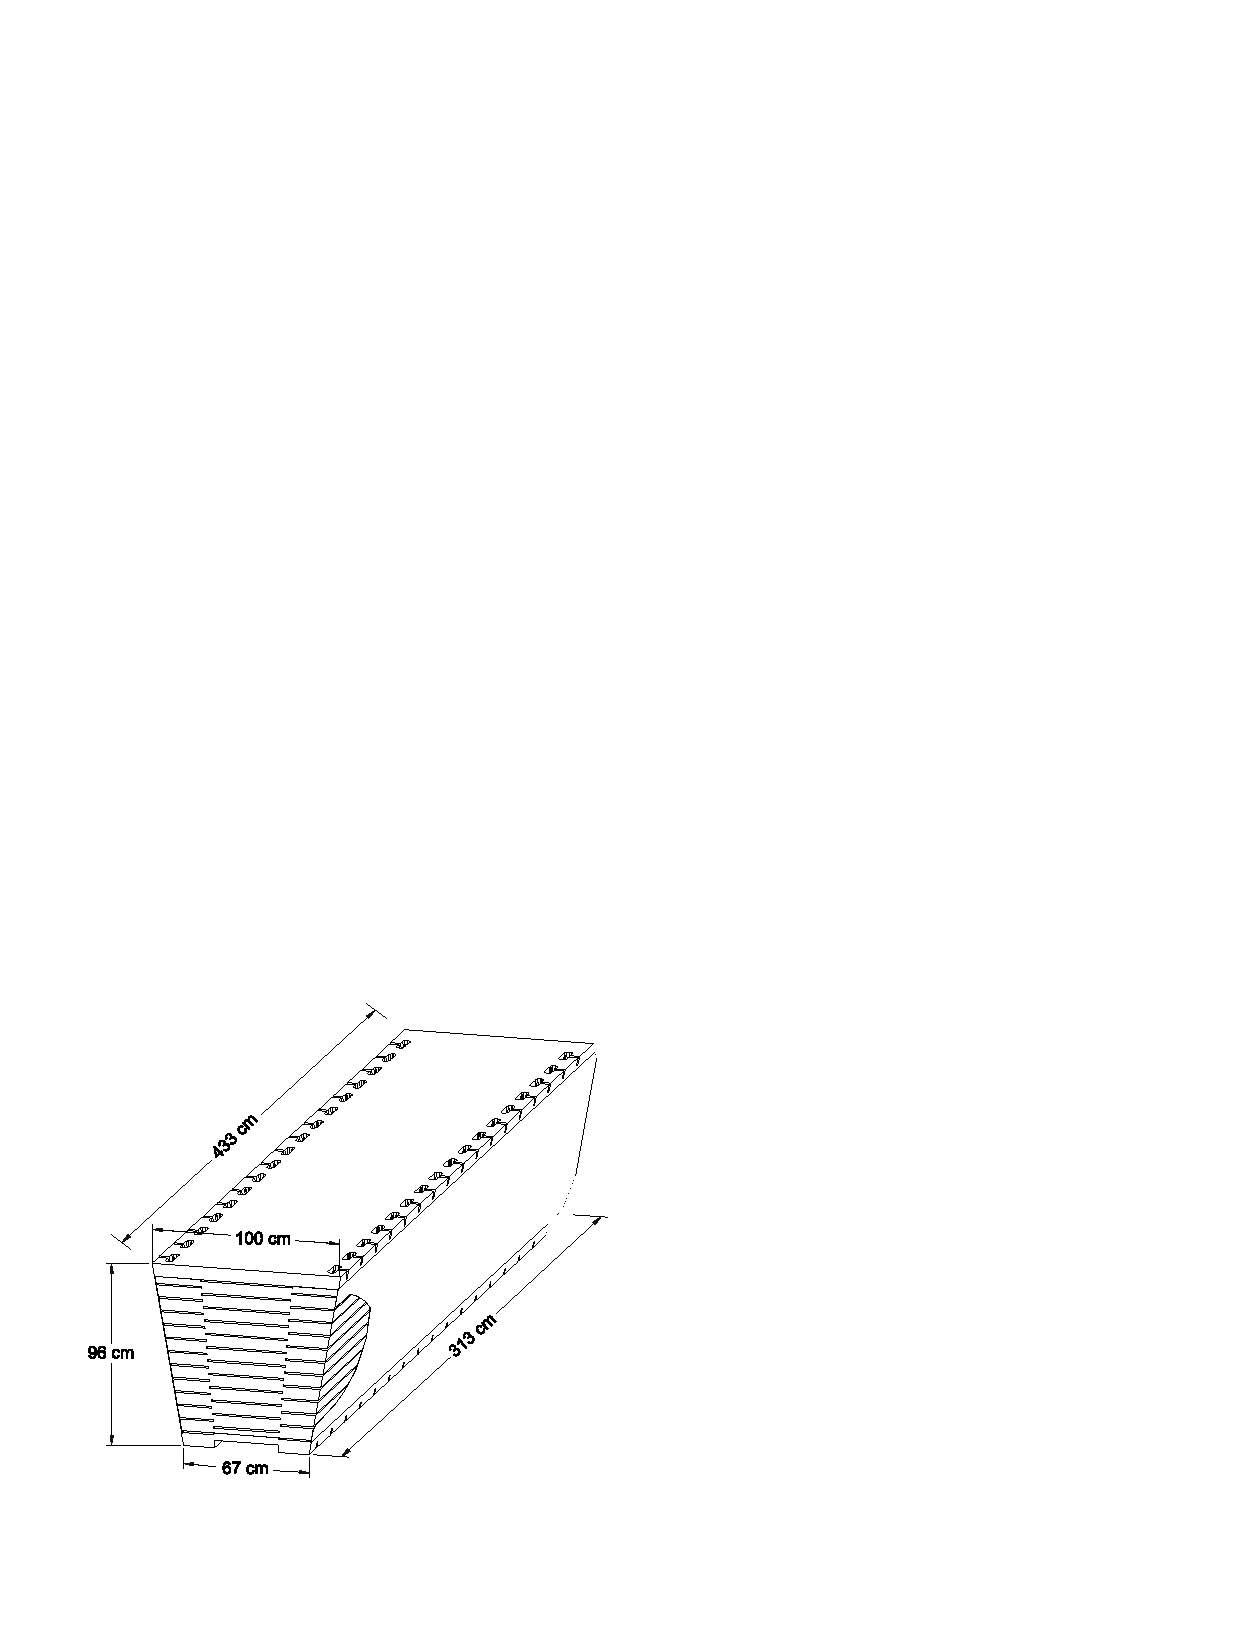
\includegraphics[width=.45\textwidth]{figures/hcal_wedge.pdf}
      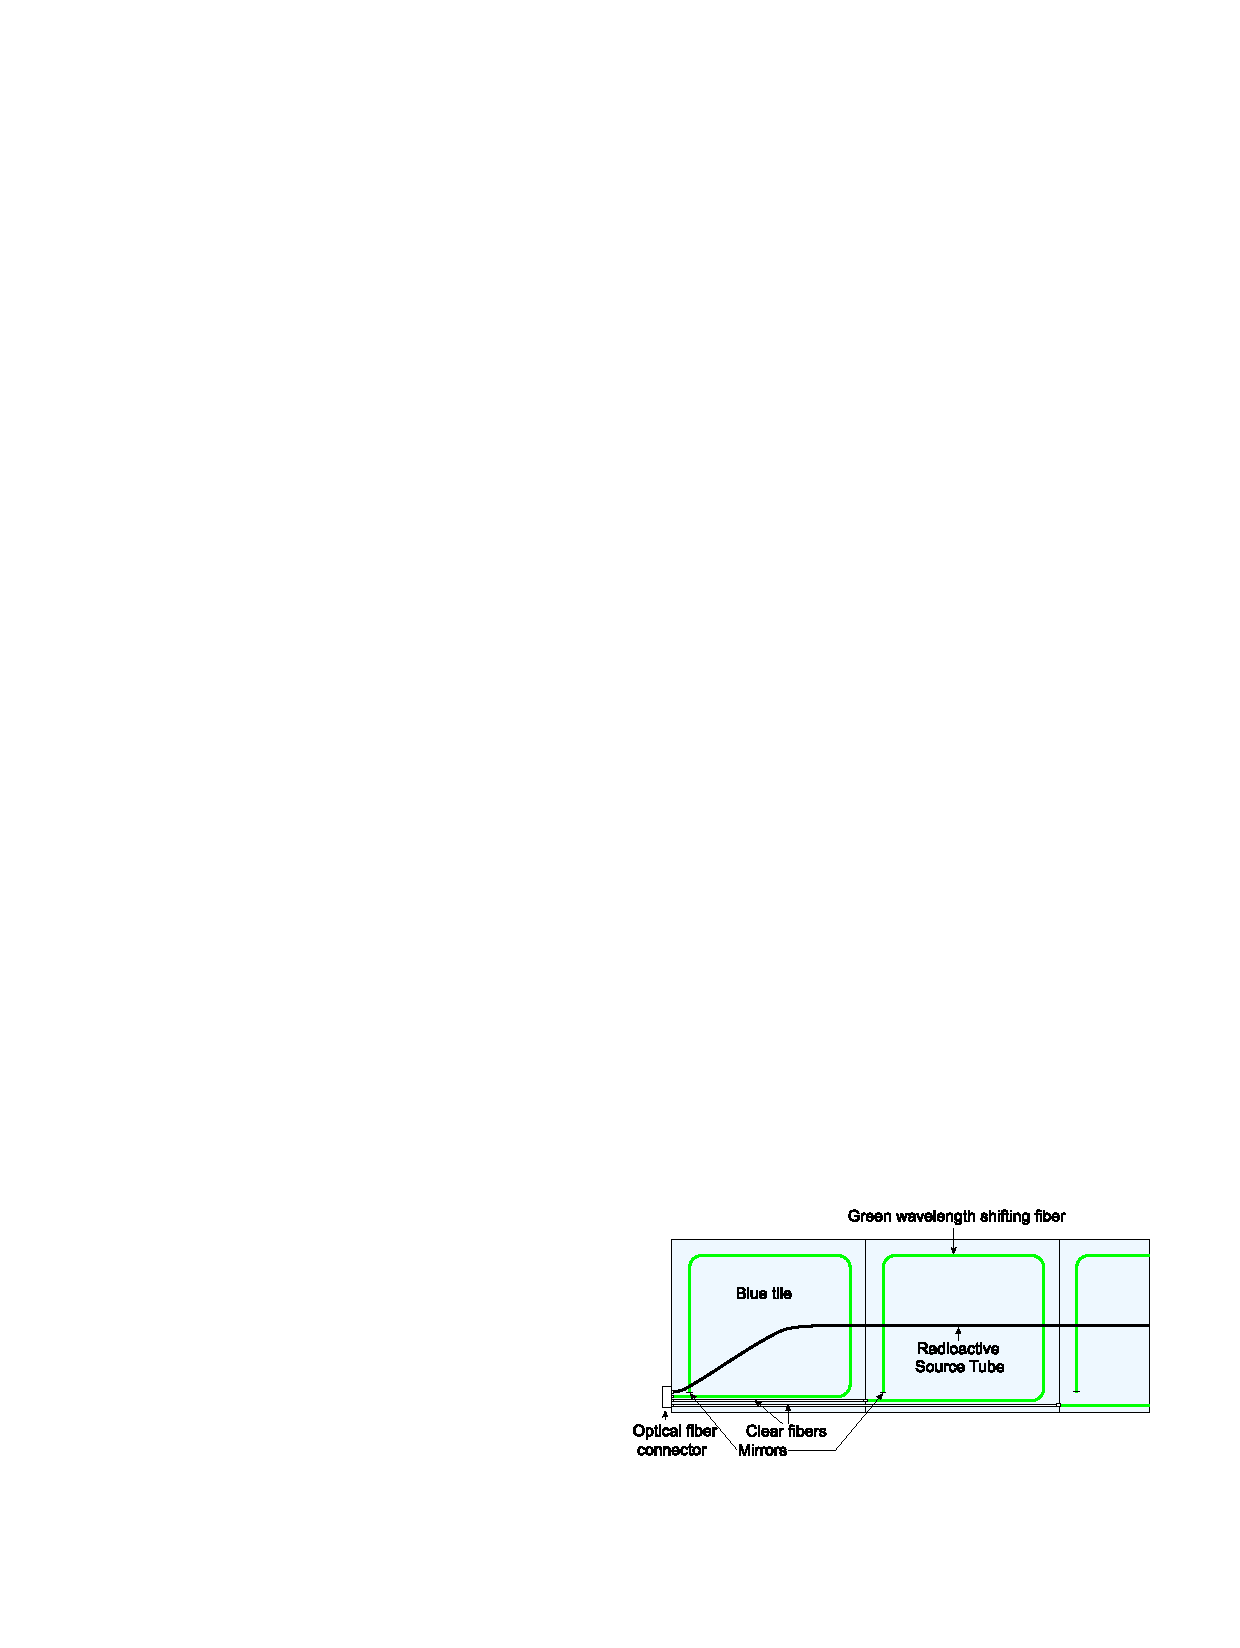
\includegraphics[width=.45\textwidth]{figures/hcal_scintillator.pdf}
      \caption{Shown on the left, a wedge of the HCAL in the barrel. The interior of the wedge is brass, and the shown slots have the scintillator modules (shown to the right) inserted so that secondary particles made in interactions with the brass will pass through them and have their energy measured. To the right, a scintillator module is shown, when a charged particle passes through the scintillator, light is generated and collected by the wavelength shifting fiber shown in green. When scintillation light is collected by the fiber, it releases green light that travels down to the clear fiber via total internal reflection and sent to be collected by photo sensors. Taken from \cite{cms_hcal_wedge}.}
      \label{fig:hcal_wedge}
    \end{figure}

    Figure \ref{fig:hcal_wedge} shows the general design of an HCAL wedge in the barrel region. Layers of brass are interspersed with scintillator strips that read out the energy of secondary particles created in the hadronic interaction. In terms of nuclear interaction lengths, the HCAL goes from about 5 nuclear interaction lengths at $\eta = 0$ up to about 10 at $\eta \ge 1.3$. Due to the shallow depth in the barrel, an outer layer of scintillator is added outside the magnet, essentially using the magnet as an absorber layer. This outer layer is called the HO and runs in the range $\eta \in [0, 1.3]$. Figure \ref{fig:hcal_layout} shows a cross-section of the HCAL including the HB, HE, and HO. With the HO in place, the minimum number of interaction lengths across the HCAL is increased to almost 12 except in the transition region between the endcap and barrel.\cite[pg. 138]{cms_jinst}

    \begin{figure}[h!]
      \centering
      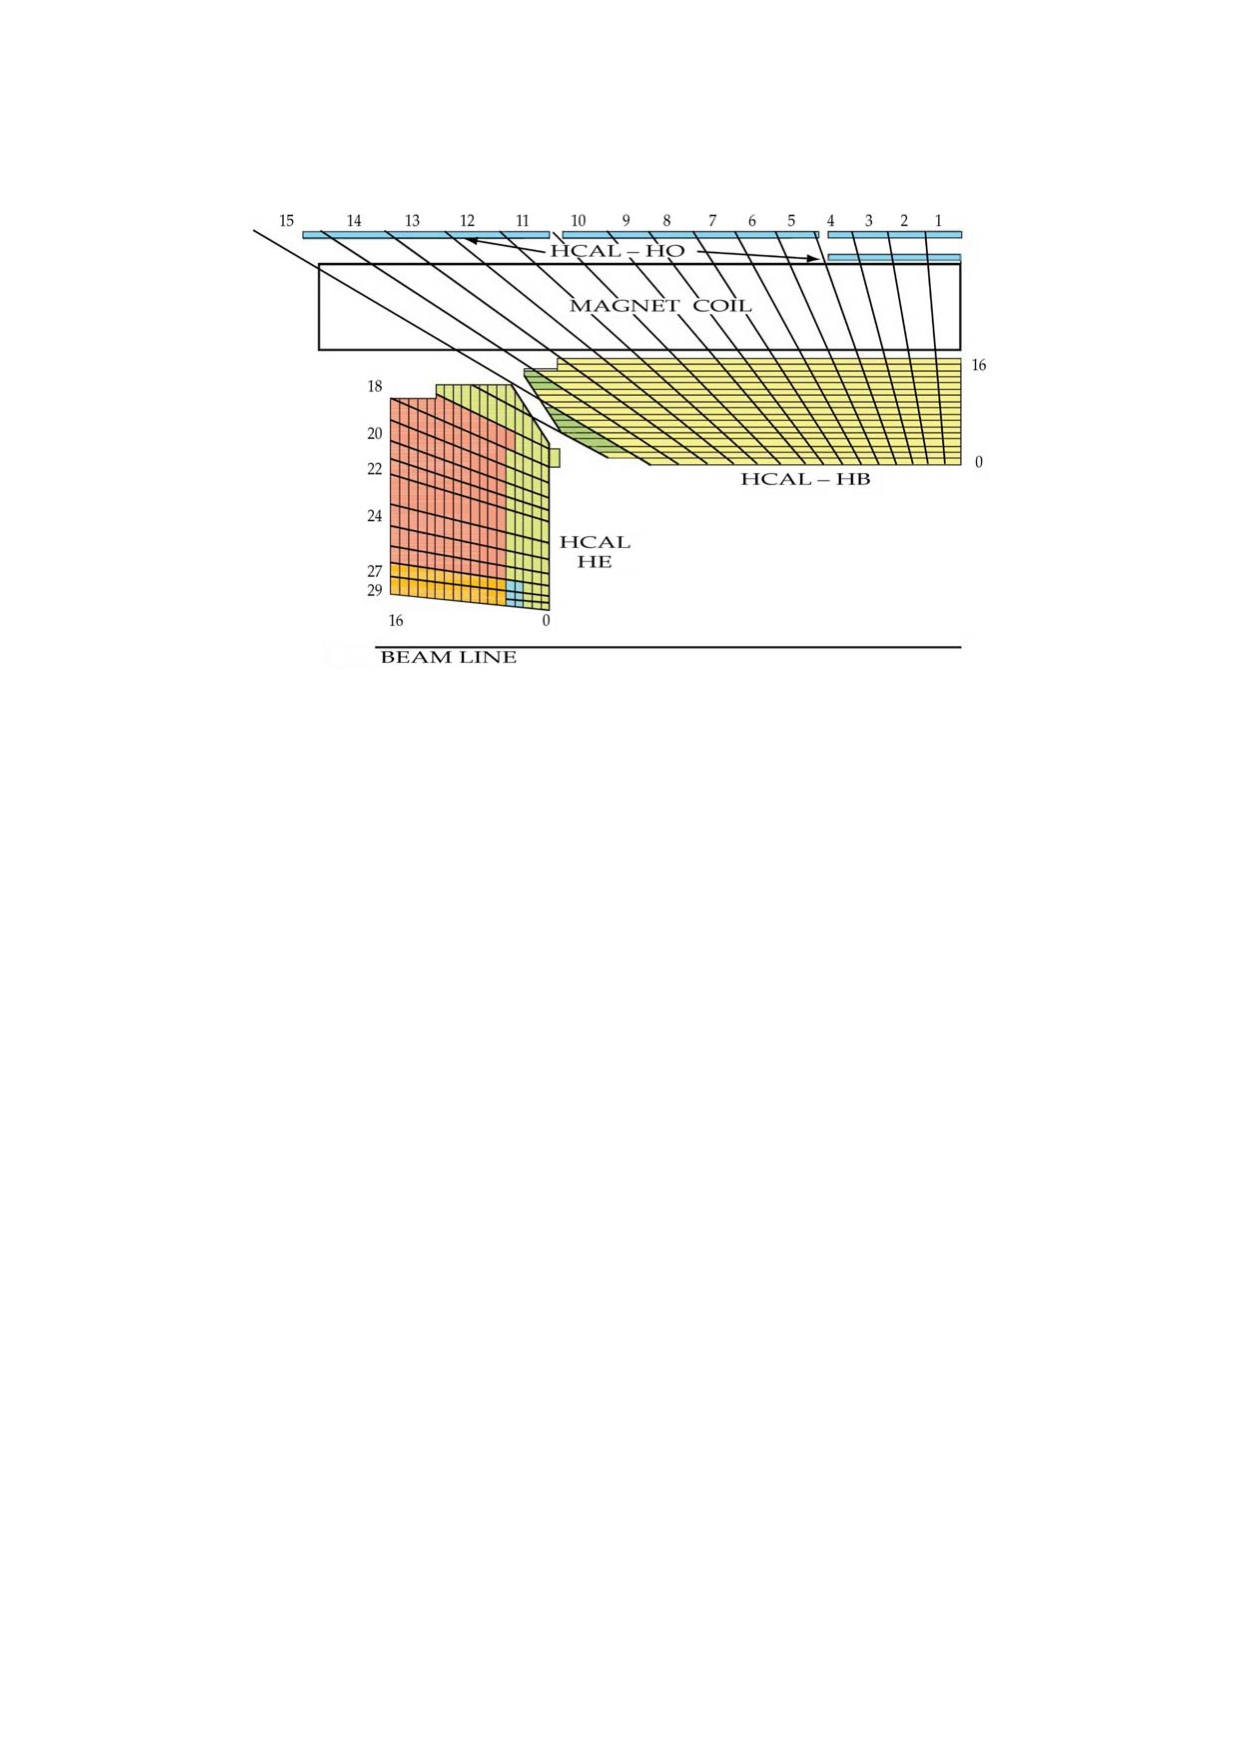
\includegraphics[width=.9\textwidth]{figures/cms_hcal_layout.pdf}
      \caption{The a cross-sectional view of the CMS hadronic calorimeter. Taken from \cite{cms_jinst}.}
      \label{fig:hcal_layout}
    \end{figure}

    Sampling calorimeters again work on the principle of scintillation, however, HCALs are meant to measure energy from neutral particles as well as charged hadrons. The strategy used in sampling calorimeters is to place dense material with many nuclei in front of the incident particles. Hadronic interactions are much more complicated than the photon and electron interactions in the ECAL because the initial state particles can vary, but in general the expected product of inelastic collisions are charged pions, which create electromagnetic cascades, and neutral particles like the $\eta$ and $\pi^0$ which quickly decay to photons. \cite[sec 35.9.2]{PDG} \cite{green_detectors} Neutron capture can also occur which makes photons that are typically out of the electronics detection capability.\todo{This is so confusing, how the hell can you say you get almost always pions for any hadronic particle?} The hadronic cascade of particles then leads into the scintillating material where scintillation light is generated and collected. Again, the amount of light collected is proportional to the energy of the charged particle \todo{why? also is the light from the $\eta$ and $\pi^0$ absorbable by the WSF?}.

    In the CMS HCAL, the absorber layers are made of brass, and the scintillator material is a proprietary plastic material, Kuraray SCSN81\footnote{excluding the very first layer where the absorber metal is stainless steel and the plastic scintillator is Bicron BC408. The very last layer also has stainless steel as the absorber metal.}. The HCAL is broken into three physical sections: the barrel (HB) extending to $\abs{\eta} \le 1.4$, the slightly overlapping endcap (HE) extending between $\abs{\eta} \in (1.3,3)$, and the slightly overlapping forward detector (HF) covering the range $\abs{\eta} \in (2.9,5)$. In this analysis, we do not use jets with energy measurements from the forward detector, that is we veto jets with $\eta > 3$.


  \subsection{The Muon System}
    The outer-most detection subsystem on CMS are the muon chamber. Muons literally put the ``M" in CMS, they are an extremely important particle for LHC physics for several reasons. \cite[sec 1.2]{muon_tdr}

    \begin{enumerate}
     \item Their production is associated with the electroweak sector, which includes the Higgs boson.
     \item They have a long enough lifetime that they can make it through the entire detector, making them easily identifiable and allowing for good momentum resolution due to their long track.
     \item Their radiative losses in the tracking system and ECAL are much smaller than electrons due to their heavier mass. They also don't deposit much energy in the HCAL because they don't interact via the strong force.
    \end{enumerate}

    The muon system on CMS is made up of three different types of detectors, all based on gas ionization.
    \begin{enumerate}
     \bitem{Drift Tubes (DTs)} Layered thin tubes with conducting cathode walls and a anode wire which runs centrally through the length of the tube. The tube is filled with Argon and CO$_2$ gas. A drift tube is shown to the left in figure \ref{fig:muon_detectors}, the length of the tube is not shown. Due to the extent in one direction, drift tubes can not give spacial resolution in all three dimensions. A typical module of these tubes has 3 layers, oriented such that the middle layer runs perpendicular to the outer layers in order to reconstruct all the position in all three dimensions. 
     \bitem{Cathode Strip Chambers (CSCs)} Six layers of anode wire planes interleaved with seven layers of cathode strips, arrayed in a cross-hatch pattern filled with gas. This configuration allows for all three dimensions of the muon's position to be reconstructed from a single module by cross referencing the voltage spikes in the strips against the voltage spikes in the wires. A schematic view of this type of detector is shown to the right in figure \ref{fig:muon_detectors}.
     \bitem{Resistive Plate Chambers (RPCs)} Parallel plate capacitors made of insulating material and filled with gas. When a muon passes through the RPC, the gas is ionized and an electron shower is generated which passes through the capacitor plates and is collected by a set of strips outside the capacitor. These detectors are interspersed throughout the entire system and mostly used to help with triggering as the response time and refractory period of these detectors are very fast compared to the 25 ns bunch crossing time. 
    \end{enumerate}

      \begin{figure}[h!]
        \centering
        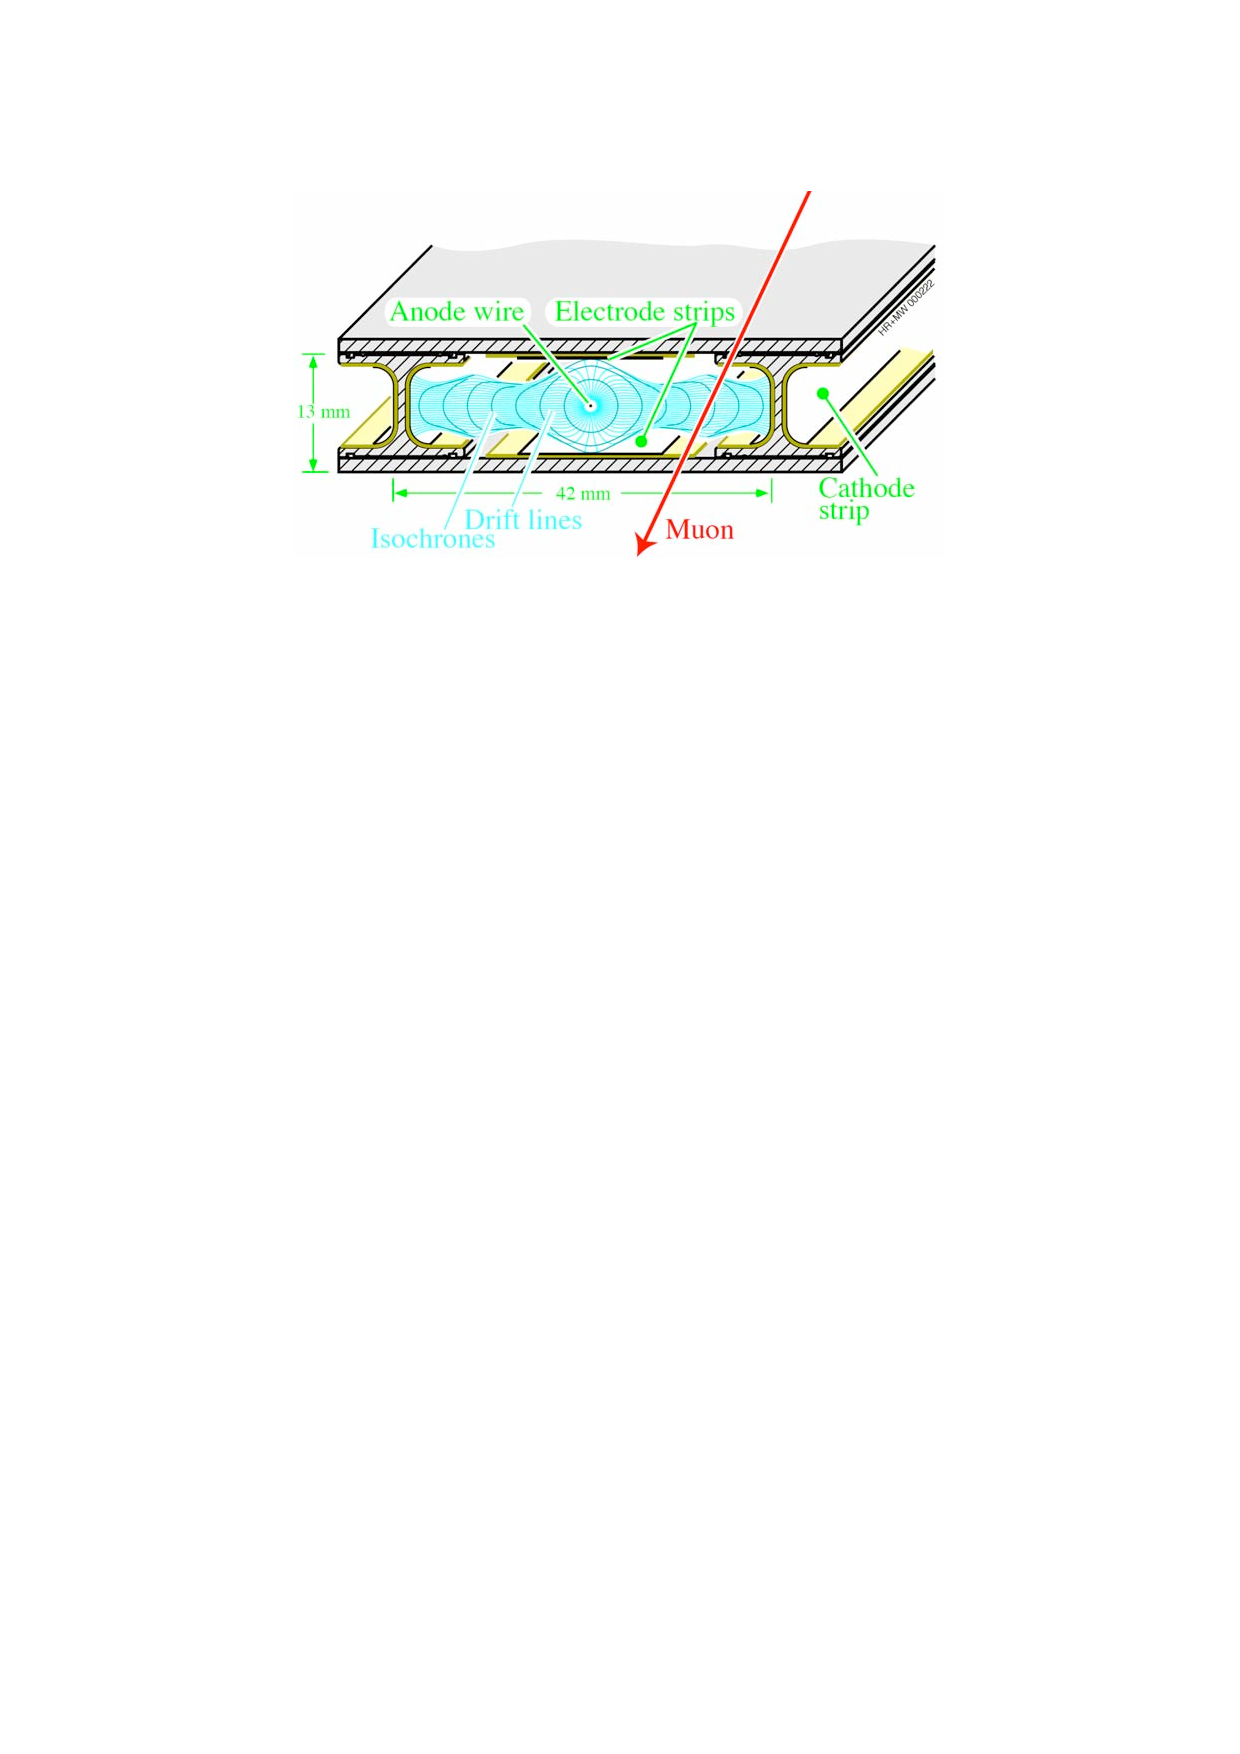
\includegraphics[width=.45\textwidth]{figures/cms_drifttube.pdf}
        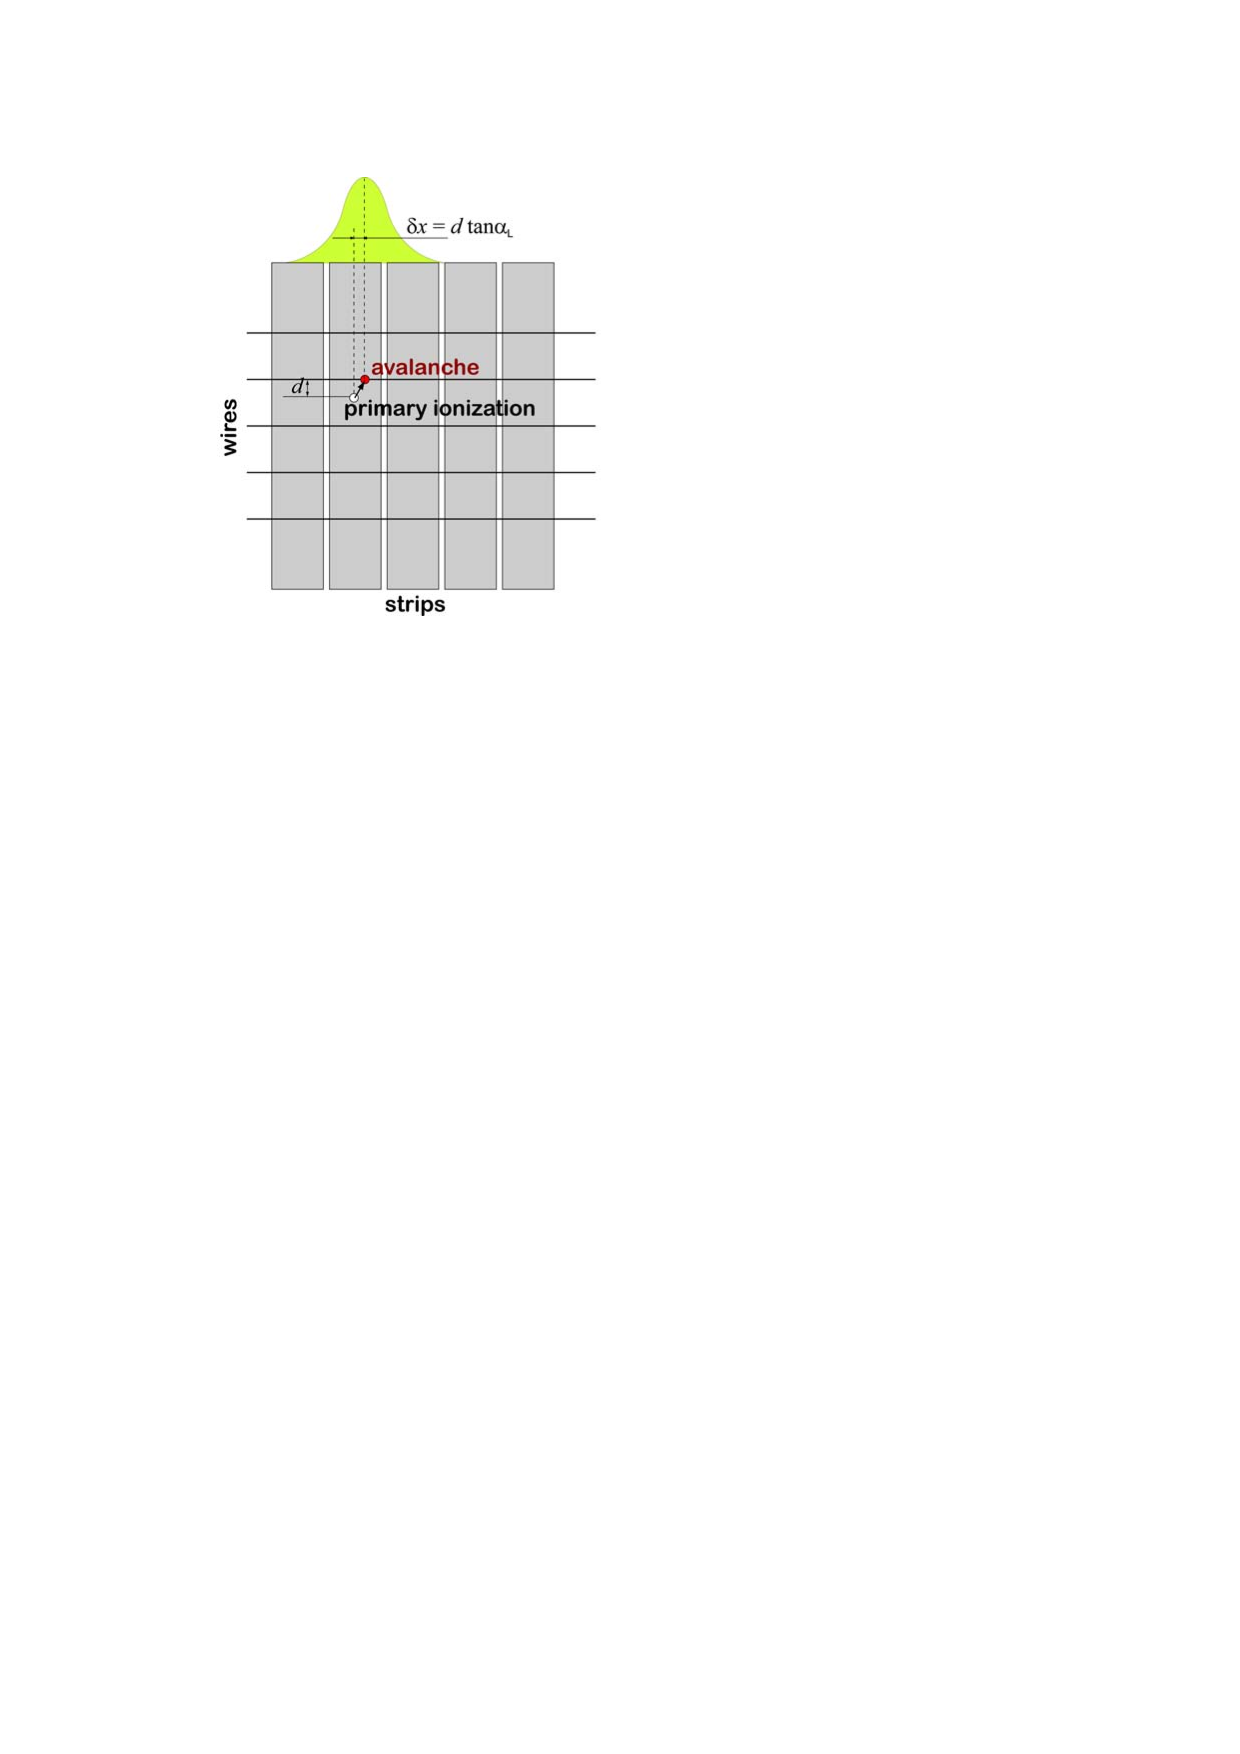
\includegraphics[width=.45\textwidth]{figures/cms_CSC.pdf}
        \caption{\textbf{Left:} A cross sectional head on view of a CMS drift tube, the tube is much longer in the omitted direction than is shown. A hypothetical path for a muon is drawn, the particle would ionize the gas in the chamber and create a spike in the potential difference between the anode and cathode as free electrons and charged ions are collected.
        \textbf{Right:} A top down view of a CSC module. A hypothetical muon hit is shown at the spot labeled ``primary ionization". A CSC module has the ability to reconstruct all three dimensions of the muon's position by cross referencing which strips collected ions and which wires collected free electrons.Taken from \cite{cms_jinst}.}
        \label{fig:muon_detectors}
      \end{figure}

      Figure \ref{fig:muon_system} shows the general layout of the muon system. In the barrel region, approximately $\abs{\eta} < 1.2$, the muon system is made up of drift tubes interleaved with RPCs. In the endcap region, approximately $\abs{\eta} \in (1.2,2.4)$, the drift tubes are replaces by CSC modules due to the higher magnetic field in this region.

    \begin{figure}[h!]
      \centering
      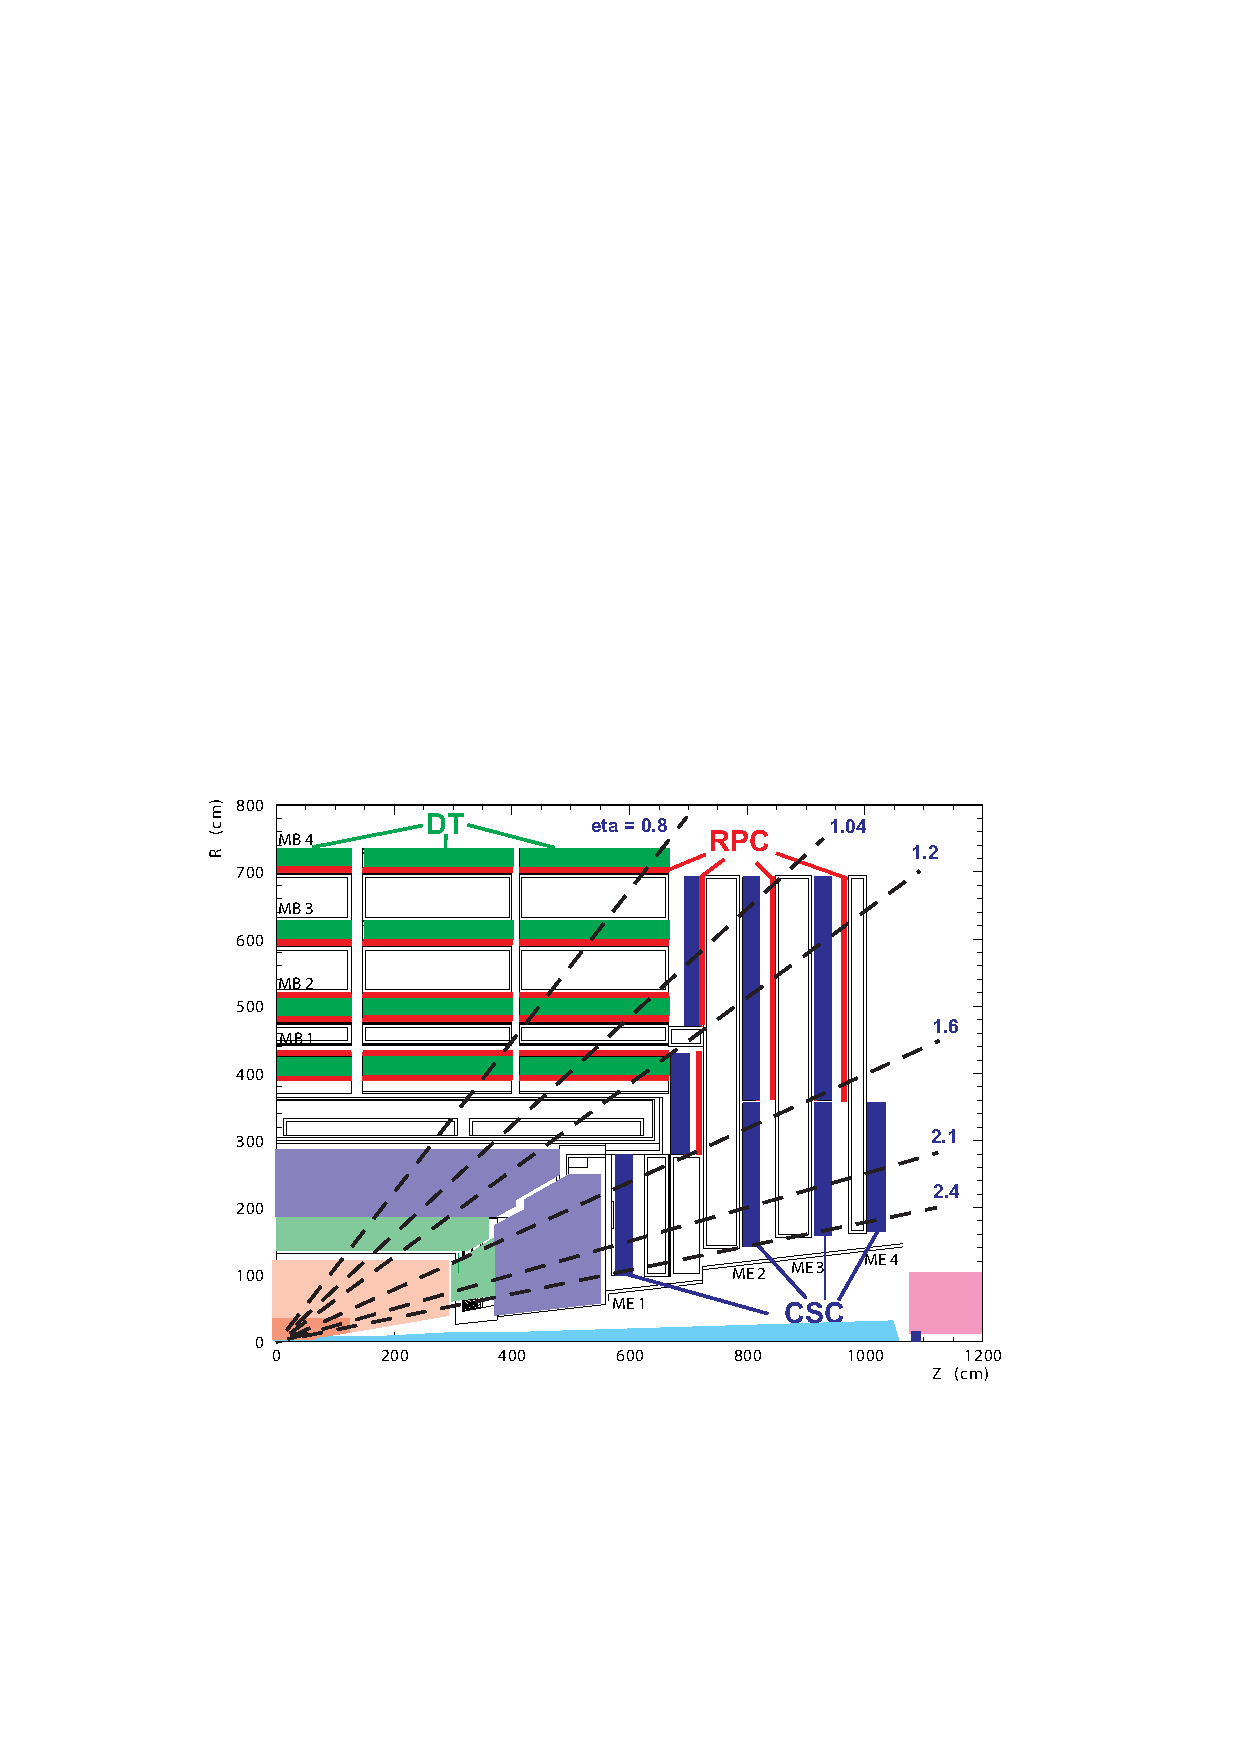
\includegraphics[width=.9\textwidth]{figures/muon_system.pdf}
      \caption{A cross-sectional view of the CMS muon system. In the barrel, with $\abs{\eta}<1.2$, drift tubes (DTs) and resistive plate chambers (RPCs) are used. In the end cap, $\abs{\eta} \in (1.2,2.4)$, RPCs and cathode strip chambers (CSCs) are used. Taken from \cite{cms_tdr}.}
      \label{fig:muon_system}
    \end{figure}

  \subsection{Event Triggering} \label{sec:event_triggering}
    A raw CMS event takes roughly 1 MB of disk space, given the rate at which bunches are crossed, storing the output from every bunch crossing would require reading out, analyzing, and storing upwards of 40 TB of data per second.\cite{trigger_tdr} The final event readout rate of the CMS detector is designed to be closer to 400 Hz, corresponding to roughly 400 MB of data per second, with the main bottleneck being offline data storage capacity and processing speed.

    In order to reduce the event rate from 40 MHz down to 400 Hz, the CMS detector employs a two-stage trigger system. The first stage, called the level 1 or L1 trigger, takes the rate down to approximately 100 kHz, a process done in hardware using application specific integrated circuits (ASICs) and field programmable gate arrays (FPGAs) for maximum speed. Events selected by the L1 system are then passed to the high level trigger system (HLT) which reconstructs physics objects in software and makes a better determination as to whether the event should be written to disk. The HLT system brings the event rate down to 100s of Hz.

    From the point of view of the L1 system, electrons and photons are identical. Decisions at level 1 for electrons and photons are made by the e/$\gamma$ L1 trigger, which mainly looks for large isolated ECAL energy deposits without a corresponding HCAL deposit. For the muon triggers, information from CSCs, DTs, and RPCs are used. Built in electronics on the detector perform track finding algorithms on hits in the DTs and CSCs independently. ``Track primitives" are created by special track finding hardware newly added for 2016. The track primitives are matched with timing and hit data from the RPCs to make decisions about muon quality and energy at L1. The processed information is sent to the global trigger system to make the final decision as to whether the event will be sent to the HLT farm.

    The HLT system consists of a processing farm with approximately 13,000 CPUs. The turn around rate for event classification is on the order of 100 ms per event. The machines in the HLT perform object identification and energy reconstruction in a way that matches the offline software suite as much as possible, though there are some optimizations made that introduce small differences to accommodate event processing at the 100 kHz rate. The HLT system is organized around the concept of ``trigger paths", which are algorithms that run object reconstruction and makes selections on these objects. A trigger path will evaluate to either true or false on an event by event basis. 

    The full list of CMS HLT trigger paths used in this analysis is presented in table \ref{table:triggers}. 

    \begin{table}[htb]
      \begin{center}
      \caption{\label{table:triggers} List of all triggers used in this analysis. }
        \begin{tabular}{l}
          \hline
          \hline
          trigger name       \\
          \hline
          di-muon triggers \\
          \hline
          --\verb=HLT_Mu17_TrkIsoVVL_Mu8_TrkIsoVVL_v*=                \\
          --\verb=HLT_Mu17_TrkIsoVVL_Mu8_TrkIsoVVL_DZ_v*=                \\
          --\verb=HLT_Mu17_TrkIsoVVL_TkMu8_TrkIsoVVL_v*=              \\
          --\verb=HLT_Mu17_TrkIsoVVL_TkMu8_TrkIsoVVL_DZ_v*=              \\
          %--\verb=HLT_TkMu17_TrkIsoVVL_TkMu8_TrkIsoVVL_DZ_v*=              \\
          --\verb=HLT_Mu27_TkMu8_v*=                                  \\
          --\verb=HLT_Mu30_TkMu11_v*=                                  \\
          %--\verb=HLT_Mu40_TkMu11_v*=                                  \\
          \hline
          di-electron triggers \\
          \hline
          --\verb=HLT_Ele17_Ele12_CaloIdL_TrackIdL_IsoVL_DZ_v*=       \\
          --\verb=HLT_Ele23_Ele12_CaloIdL_TrackIdL_IsoVL_DZ_v*=       \\
          --\verb=HLT_DoubleEle33_CaloIdL_GsfTrkIdVL_v*=           \\
          --\verb=HLT_DoubleEle33_CaloIdL_GsfTrkIdVL_MW_v*=           \\
          \hline
          e$\mu$ triggers \\
          \hline
          --\verb=HLT_Mu17_TrkIsoVVL_Ele12_CaloIdL_TrackIdL_IsoVL_v*= \\
          --\verb=HLT_Mu23_TrkIsoVVL_Ele8_CaloIdL_TrackIdL_IsoVL_v*= \\
          --\verb=HLT_Mu23_TrkIsoVVL_Ele12_CaloIdL_TrackIdL_IsoVL_v*= \\
          --\verb=HLT_Mu23_TrkIsoVVL_Ele8_CaloIdL_TrackIdL_IsoVL_DZ_v*= \\
          --\verb=HLT_Mu23_TrkIsoVVL_Ele12_CaloIdL_TrackIdL_IsoVL_DZ_v*= \\
          --\verb=HLT_Mu8_TrkIsoVVL_Ele17_CaloIdL_TrackIdL_IsoVL_v*=  \\
          --\verb=HLT_Mu8_TrkIsoVVL_Ele23_CaloIdL_TrackIdL_IsoVL_v*=  \\
          --\verb=HLT_Mu8_TrkIsoVVL_Ele23_CaloIdL_TrackIdL_IsoVL_DZ_v*=  \\
          %--\verb=HLT_Mu12_TrkIsoVVL_Ele23_CaloIdL_TrackIdL_IsoVL_v*=  \\
          %--\verb=HLT_Mu12_TrkIsoVVL_Ele23_CaloIdL_TrackIdL_IsoVL_DZ_v*=  \\
          --\verb=HLT_Mu30_Ele30_CaloIdL_GsfTrkIdVL_v*=               \\
          --\verb=HLT_Mu33_Ele33_CaloIdL_GsfTrkIdVL_v*=               \\
          \hline
          single-$\gamma$ triggers \\
          \hline
          --\verb=HLT_Photon22_R9Id90_HE10_IsoM_v*=  \\ 
          --\verb=HLT_Photon30_R9Id90_HE10_IsoM_v*=  \\
          --\verb=HLT_Photon36_R9Id90_HE10_IsoM_v*=  \\
          --\verb=HLT_Photon50_R9Id90_HE10_IsoM_v*=  \\
          --\verb=HLT_Photon75_R9Id90_HE10_IsoM_v*=  \\
          --\verb=HLT_Photon90_R9Id90_HE10_IsoM_v*=  \\
          --\verb=HLT_Photon120_R9Id90_HE10_IsoM_v*= \\
          --\verb=HLT_Photon165_R9Id90_HE10_IsoM_v*= \\
          --\verb=HLT_Photon165_HE10_v*=             \\
          \hline
          single-$\mu$ triggers \\
          \hline
          --\verb=HLT_IsoMu24_v*=  \\ 
          --\verb=HLT_IsoTkMu24_v*=  \\ 
          \hline
          \hline
        \end{tabular}
      \end{center}
    \end{table}

    The high level triggers are generally based on isolation and transverse momentum criteria. For instance, the trigger HLT\_Mu17\_TrkIsoVVL\_Mu8\_TrkIsoVVL\_DZ\_v* roughly requires that the event have at least one muon above 17 GeV of \pt and another above 8 GeV. The tags TrkIsoVVL refer to isolation requirements on the muon and DZ refers to a requirement that when their tracks terminate close to one another in the z (beamline) direction traced back to the beamline. The v* at the end of these triggers denotes that we use the latest version of the software that implements the trigger. \todo{if I get more info on the trigger tags, I'll add it here.}

    \subsubsection{Trigger efficiencies} \label{sec:trigger_efficiencies}
    Due to the low precision in the energy measurements at level 1, and the slight differences in reconstruction at the HLT and offline level \todo{is this right?}, objects near the \pt thresholds of the high level trigger do not always cause the event to be stored, we say that the triggers are not 100\% efficient. In other words, sometimes an event with an electron that is reconstructed to have 17 GeV of \pt offline will not pass the Ele17 trigger because it was either not selected at level 1, or it was reconstructed to have less \pt than 17 GeV by the HLT reconstruction software.

    The rate at which this occurs can be treated statistically. It is mainly a function of the offline reconstructed \pt because all of the triggers used in this analysis are based on the \pt of some object. As an example, figure \ref{fig:mu_l1_eff} shows the L1 trigger efficiency for the single muon L1 25 GeV trigger in the 2017 dataset\footnote{this analysis uses the 2016 dataset, the figure is only for illustration} at the \pt threshold of 25 GeV (the target threshold for the single muon trigger). As can be seen in the figure, muons with \pt $\le 8$ GeV (as reconstructed offline) are almost never selected by the 25 GeV L1 trigger. The trigger never selects 100\% of the muons, even at very high energies. However, after about 30 GeV, the percentage of muons selected plateaus. We say that the trigger is \emph{fully efficient} at 30 GeV to denote this feature, which is common to all trigger turn-on curves.

    \begin{figure}[h!]
      \centering
      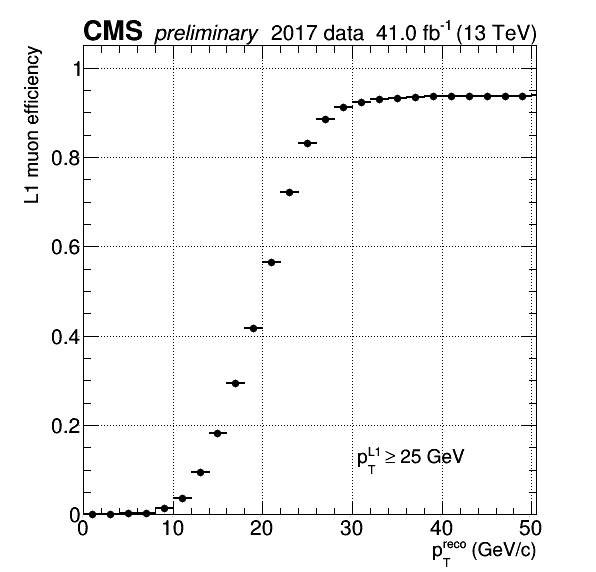
\includegraphics[width=.7\textwidth]{figures/muon_l1_eff.png}
      \caption{The trigger efficiency for the L1 muon 25 GeV trigger. The system attempts to pass all muons with 25 GeV of \pt to the HLT system, though the fast calculation with on-board hardware at L1 does not capture all muons at this threshold. The plot is made by selecting events with two muons reconstructed offline where the leading \pt muon has \pt above 27 GeV and has passed the L1 25 GeV trigger. The second muon is then checked to see whether it also passed the L1 criteria. This method is called tag-and-probe. As can be seen, the trigger is never at 100\% efficiency, but a plateau exists around 30 GeV where we call the trigger \emph{fully efficient}. Taken from \cite{mu_l1_twiki}.}
      \label{fig:mu_l1_eff}
    \end{figure}

    Trigger efficiencies enter this analysis in two places. First, MC used in this analysis has the trigger efficiencies built in, that is MC events are tagged as passing for failing triggers at rates equal to the trigger efficiencies. Second, the difference in the efficiencies for the electron and muon trigger paths in this analysis are part of what is corrected by the \rsfof factor, which will be described in section \ref{sec:rsfof}. In short, this analysis uses the symmetry between production rates of electrons and muons in certain physics processes to make certain background predictions. That symmetry is broken by the fact that, along with different offline ID requirements, the trigger efficiencies for electrons and muons at the same \pt will, in all likelihood, not be identical.

\section{Physics Objects}
  After energy deposits are read out from the detector they are used to reconstruct \emph{physics objects} that can then be further analyzed to discover new particles and interactions. The layout of the CMS detector was chosen carefully to allow for the identification of several groups of particles:

  \begin{enumerate}
    \bitem{Jets} sprays of particles containing mostly hadrons and photons. An ideal jet will leave multiple tracks in the tracker that point back to the same spot on the beamline and deposit a large amount of energy in the HCAL and a smaller amount of energy in the ECAL as well.
    \bitem{Isolated Photons} single photons that were likely produced in the hard collision, rather than being radiated by a charged particle in the detector. An ideal single photon will leave no tracks and deposit energy in only the ECAL
    \bitem{Isolated Electrons} single electrons that were likely produced in the hard collision, rather than being produced as a secondary particle in the detector (for instance in pair production). An ideal isolated electron will leave a hit in every layer of the tracker and deposit energy only in the ECAL along the line traced out by the tracker hits. Bremsstrahlung photons are typically radiated from electrons in the tracker, therefore we should also expect kinks in electron tracks accompanied by energy deposits in the ECAL associated with the kinks.
    \bitem{Muons} expected to leave hits in every layer of the inner tracker. When extrapolated through the detector, the inner tracker hits should match up with standalone muon tracks in muon system. Nearly no energy should be deposited in the ECAL or HCAL
    \bitem{Tagged Jets} jets that have been tagged as originating from a specific particle, for instance a b-quark or a $\tau$-lepton. These objects typically use information from the jet tracks to give a measure of how likely a specific jet was to represent the decay dynamics of the specific particle in question.
  \end{enumerate}

  In order to reconstruct these objects from energy deposits in the detector, CMS employs an algorithm called particle flow\cite{cms_particleflow} which will be outlined in section \ref{sec:particle_flow}. However, the first step in object generation is the vertex and track reconstruction.

  \subsection{Track Reconstruction} \label{sec:track_reconstruction}
    Track reconstruction is the process of turning hits in the tracker into proposed trajectories for charged particles. The track finding software used by CMS is called the Combinatorial Track Finder \cite[pg. 12]{cms_track_vertex}, which is based off of the Kalman filter \cite{kalman_filter} track fitting method. The basic idea is to work iteratively, first building the more ``obvious" tracks for high \pt particles, and then removing their hits from the collection thus making the next track easier to find.

    Each iteration begins with a ``seed track." In the first iteration, the seed tracks are built from collections of 3 hits, one in each layer of the pixel tracker, with curvature tolerance such that the particle \pt is larger than 0.8 GeV. In later iterations, seed tracks are built from hit groups that are missing a layer in the pixel tracker, or even from hit groups solely in the strip tracker to accommodate the possibility of secondary decays.

    The seed tracks are extrapolated into the next layer of the tracker, taking into account the uncertainty in the track's position and momentum, by assuming a constant magnetic field and disregarding the possibility of multiple scattering and energy loss when the particle is not within a tracker layer\footnote{Energy loss is modeled statistically when the particle is in the tracker material, which has the effect of broadening the track uncertainty.}. After the expected trajectory is built, hits within some number of standard deviations of the expected trajectory in the nearest tracker layer are collected into groups of possible energy deposits for the particle\cite{track_uncertainty}. This process can include the possibility of adding a ``ghost hit" if no hit was found in a module along a particular possible trajectory. 

    A $\chi^2$ test is then performed between the expected trajectory and the hit groups, taking into account the hit and trajectory uncertainties. The number of hits in a typical event is enough that most seed trajectories can be associated with multiple paths at each layer. After possible trajectories are built out of the hit groups, only a small number of possible trajectories are extrapolated into the next layer based on their $\chi^2$ values and number of ghost hits. This process is repeated until track quality parameters, for instance too many ghost hits, can no longer be satisfied at the next layer. After the hits in the detector are organized into tracks, another fit is applied to smooth the track trajectory using a Kalman filter fit. During this stage, hits which are outliers can be disassociated with the trajectory and added back the general collection of hits. The smoothing step occurs again until all outliers have been removed\cite[sec 4.3]{cms_track_vertex}.

  \subsection{Vertex Selection} \label{sec:vertex_selection}
    Each event recorded at CMS has a \emph{primary vertex}, which is roughly defined as the point along the beamline at which the highest energy tracks emerged. This process involves first selecting the highest quality tracks from track reconstruction, then clustering them into sets that seem to originate from roughly the same point along the beamline, and finally fitting the location of the vertex based on the cluster end-points. 

    Tracks are selected based on the impact parameter to the beamline ($<$5), number of hits ($\ge 2$ pixel, $\ge 5$ pixel+strip), and the $\chi^2$ value from the track fit ($<20$). Again the vertex selection is an iterative process, at first all tracks are assumed to come from one vertex, then at each step vertices can be split. In practice this is achieved with a process called \emph{deterministic annealing} (DA) which is based on ideas from thermodynamics of minimizing free energy at some temperature. 

    Once vertices are identified and tracks are assigned to a vertex, vertices with at least two tracks are fitted using an adaptive vertex fitter \cite{adaptive_vertex_fitter} to compute position and quality quantities such as the position of the vertex in space and weights for the likelihood that the tracks associated with the vertex genuinely began there. The weight, $w_i$, of a track $i$ is close to 1 if its position is near the vertex and close to 0 if its position is several standard deviations away. The quantity \ndof is used a quality parameter defined as

    \[
      \ndof = -3+2 \sum \limits_{i=1}^{\text{\# tracks}} w_i.
    \]

    When more than one primary vertex can be found in an event, the vertex with the highest scalar sum of \pt for all the tracks associated with the vertex is chosen. In the analysis presented in this thesis, we only select events where the primary vertex has \ndof $>4$, and the vertex is located within 24 cm from the center of the detector along the beamline direction and within 2 cm from the beamline in the transverse plane.

  \subsection{Particle flow} \label{sec:particle_flow}
    The particle flow algorithm is in charge of turning tracks and energy clusters from the calorimeters into physics objects with energy, momentum, and location information. It achieves this goal through an iterative process of linking energy deposits, much like the tracking algorithm outlined above in sec \ref{sec:track_reconstruction}. Energy deposits in the Calorimeters, tracks in the inner tracker, and tracks in the muon chambers are all linked together pairwise based on various criteria \cite[sec. 4]{cms_particleflow}. The exact criteria for particle flow identification can be found in detail in the previous citation. In broad strokes, the energy deposits in the detector are turned into electrons, photons, muons, charged hadrons, and neutral hadrons based on the following criteria:

    Electrons are identified when tracks in the inner tracker are linked with energy deposits in the ECAL. When such a link is found, a Gaussian Sum Filter (GSF) \cite{cms_gsf} algorithm reconstructs the track because kinks in electron tracks due to bremsstrahlung radiation are not handled well by the standard Kalman Filter tracking as it does not account for momentum changes due to radiation. An energy deposit in the ECAL without a corresponding track is reconstructed as a photon. Muons are reconstructed by comparing tracker muons, tracks in the inner tracker with at least one associated hit in the muon system, with standalone muons, reconstructed tracks in the muon system. Reconstruction of a muon requires a tracker muon and a standalone muon with compatible trajectories and the absence of a large energy deposit in the calorimeters. Finally, energy deposits in the HCAL are considered neutral hadrons, and tracks which leave energy deposits in the HCAL, but not the ECAL, are considered charged hadrons.

    After the energy deposits are clustered into particles, we use the anti-KT algorithm with a radius of $R=0.4$ in $(\eta, \phi)$ space to cluster particles into jets.\cite{cms_jet_performance} 


  \subsection{Electron Measurement Pipeline} \label{sec:electron_measurement_pipeline}
    High energy electrons have energy measurements based mainly on their ECAL deposit. When a charged particle moves through the tracker, a momentum measurement can be found due to its curvature. However, due to the likelihood of bremsstrahlung radiation, the sagitta of an electron track has a high chance of being malformed, containing kinks caused when a high energy photon is emitted. Since the sagitta momentum measurement assumes the free motion of a charged particle in a magnetic field with constant energy, the track from an electron that emits a high energy photon can not be used to determine the electron's original momentum.

    When the electron reaches the ECAL, almost all of its energy is deposited within a small region. For instance, a 120 GeV electron typically deposits 95\% of its energy within a 5x5 crystal array. However, when passing through the tracker, an electron will radiate 33\% of its energy an average before it reaches the ECAL, this figure inflates to about 86\% of the energy for electrons that pass through the densest parts of the detector near $\abs{\eta} = 1.4$ (seen in fig. \ref{fig:tracker_material_budget}). Due to the bending of the electron in the magnetic field, bremsstrahlung photons will tend to spread out in the $\phi$ direction, with the spread in the $\eta$ direction being mostly negligible \cite[sec. 4.1]{Electron_reco}.

    In addition to the momentum measurement, the Kalman Filter track building method is poorly suited for electron tracks as it also assumes the motion of constant energy charged particle in a magnetic field. In order to construct electron tracks, CMS also utilizes another track finding algorithm developed specifically for the reconstruction of electron tracks called the Gaussian Sum Filter (GSF)\cite{cms_gsf}, which can be roughly intuited as several Kalman Filters assuming different radiation rates running in parallel. 

    A high energy photon radiated by an electron will leave an energy deposit in the ECAL and change the trajectory curvature for the electron. These deposits can typically be found by tracing tangents from the electron's trajectory to the ECAL due to the high likelihood that bremsstrahlung photons will be emitted along the electrons momentum vector \todo{can I find a source that says how much this is true as a function of energy?}. 

    To measure the total energy of the electron, the energy of the bremsstrahlung photons should be included as well, and so the ECAL clusters energy deposits into \emph{superclusters}. Track reconstruction with the GSF algorithm is similar to that of the Kalman filter described in sec. \ref{sec:track_reconstruction}, but, in addition to seeding tracks from pixel hits, ECAL superclusters are also used as seeds and tracks leading into the end of a supercluster are extrapolated backwards towards the beamline assuming both charge hypotheses. \todo{is there consistency checking that the photons come at places where there are reasonable kinks?} Ultimately, the electron's momentum is reconstructed using a weighted combination of the track momentum and supercluster energy. Electrons with energy less than 15 GeV use almost exclusively the pixel track momentum, while electrons with energy greater than 250 GeV use the supercluster measurement exclusively. 

    A series of corrections are applied to the supercluster energy. These corrections are derived in simulation where true electron energies and momenta are known to perfect precision. They include the effect of deposited energy not being properly associated the supercluster, loss of energy due to gaps in and between detector modules, pileup, and so on.\cite[sec 4.8]{Electron_reco} 

    Differences in data and simulation are due mainly to imperfect modeling of the tracker material. Figure \ref{fig:electron_Z_resolution} shows the dilepton mass of Z$\to$ee events in both data and simulation. The events in data are estimated to have 2\% background contamination\cite[sec. 4.5.1]{ecal_energy_reco} and are selected by requiring two opposite charge electrons with dilepton mass in the range 60-120 GeV, and where each lepton has at least 25 GeV of \pt. These comparisons are made for different ranges of $\eta$ and \pt as well as instantaneous luminosity and ``quality class" based on the scale and number of bremsstrahlung photon deposits found in the electron's supercluster. Although the agreement between data and simulation is excellent, a correction is applied to data so that the overall energy scale matches that seen in simulation, and a correction is applied to simulation so that the energy resolution matches that seen in data. \todo{What does it mean for the simulation correction? Where is that propagated?}

    \begin{figure}[h!]
      \centering
      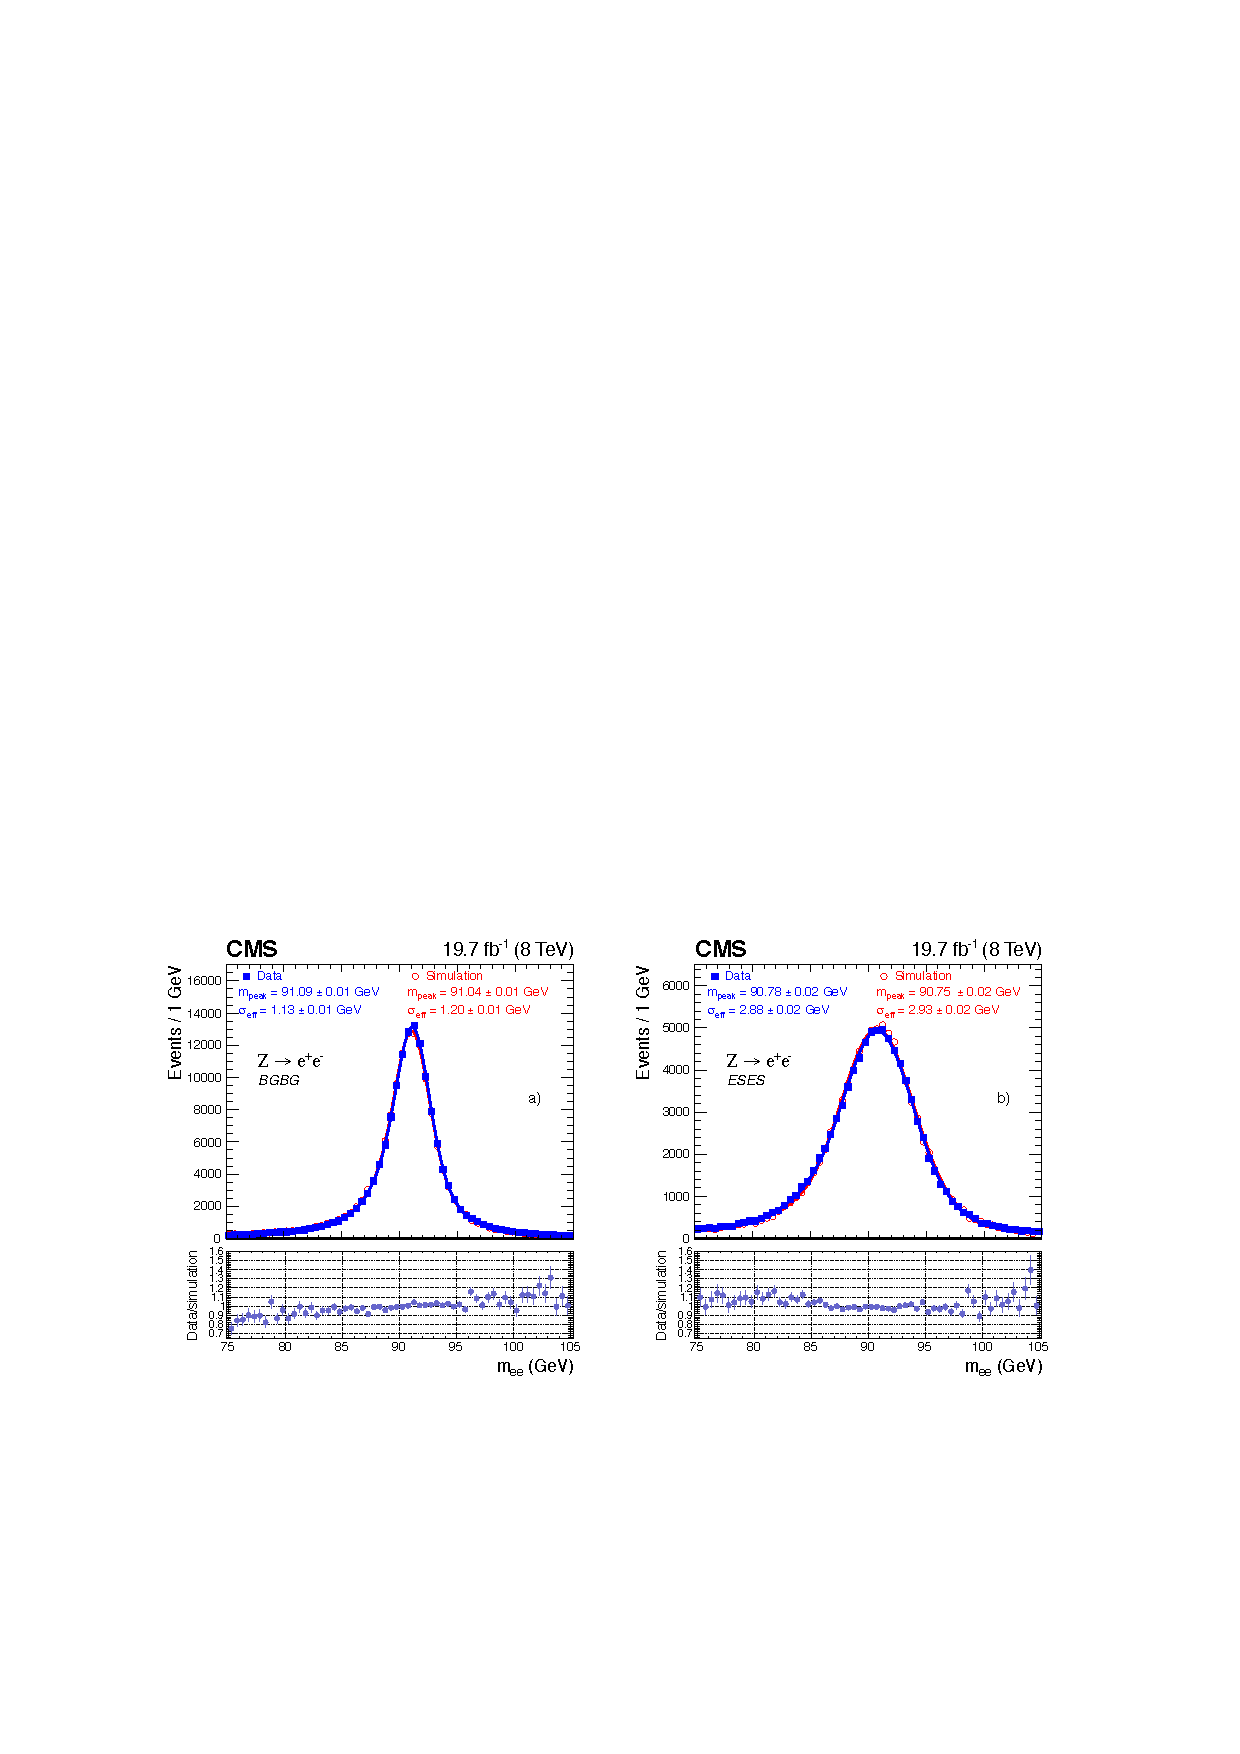
\includegraphics[width=.7\textwidth]{figures/electron_Z_resolution.pdf}
      \caption{Data and simulation of Z to di-electron events at 8 TeV. On the left, only electrons in the barrel which have not undergone any bremsstrahlung radiation are plotted, these should be the easiest class of electrons to measure. To the right, only electrons in the endcap with multiple subclusters in their ECAL supercluster are plotted, these should be the hardest class to measure. In both cases there is excellent agreement between data and simulation meaning that the corrections applied to data derived from simulation are reasonable. Additionally, the peak Z masses match the established value to approximately the percent level in both cases. Taken from \cite{Electron_reco}.}
      \label{fig:electron_Z_resolution}
    \end{figure}

  \subsection{Muon Measurement Pipeline} \label{sec:muon_measurement_pipeline}
    Muon reconstruction starts with tracks from the inner and tracker and muon system. Muon identification in particle flow can come from several sources, but in this analysis we only use ``global muons". 

    Tracks found in the muon system are called ``standalone muons." For each standalone muon track, a collection of possible tracks in the inner silicon tracker that could correspond to the standalone muon are identified. These tracks are then propagated forward to a common plane with the standalone muon track which is propigated backwards to the same plane. Position information on that plane, along with momentum measurements and uncertainties are used to select the best match. \cite[sec 3]{cms_muons} \cite[sec 5.1]{muon_reco_AN} After a match is found, the Kalman Filter track fitting method is applied from scratch to the hits in the inner tracker and muon system to smooth the overall combined track, which constitutes the global muon track used in this analysis.

    Muon momenta are computed from the sagitta of the track. At high energies, the segment of the track in the tracker provides the best momentum resolution due to the tighter density of the inner tracker modules. At energies above approximately 200 GeV, the tracks in the muon system provide a better measurement due to their longer lever arm. \todo{Is this correct?} 

    Again, a series of corrections to the muon momentum are derived using simulation. Because the measurement of the momentum is done via the track sagitta, as explained in appendix \ref{sec:sagitta}, the largest source of mismeasurements comes from misalignment of the tracker and muon modules, incorrect modeling of the magnetic field, and mis-modeling of the tracker material.\cite[sec. 6]{cms_muons} In general, the CMS detector is built to ensure that the energy resolution of muons (measured in terms of their \pt) is good to within 1\% for a 100 GeV muon and 10\% for a 1 TeV muon. In other words, CMS was built with the requirement that $\frac{\sigma(\pt)}{\pt} \approx 0.01$ for $\pt \approx 100$ GeV and $\frac{\sigma(\pt)}{\pt} \approx 0.1$ for $\pt \approx 1$ TeV. 

    Figure \ref{fig:muon_Z_resolution} shows the results of the SIDRA study that don't actually tell you anything about the energy resolution.

    \todo{Looks like this isn't what we actually get though, that figure is WAAAYAYYYYYY worse than 1\%. Why does CMS not make a fucking plot that says, here's what the Z peak is supposed to look like, here's what our fucking data says? Why? Probably because it would show that no one knows what the fuck they are doing and all of our analyses are garbage.}

    \begin{figure}[h!]
      \centering
      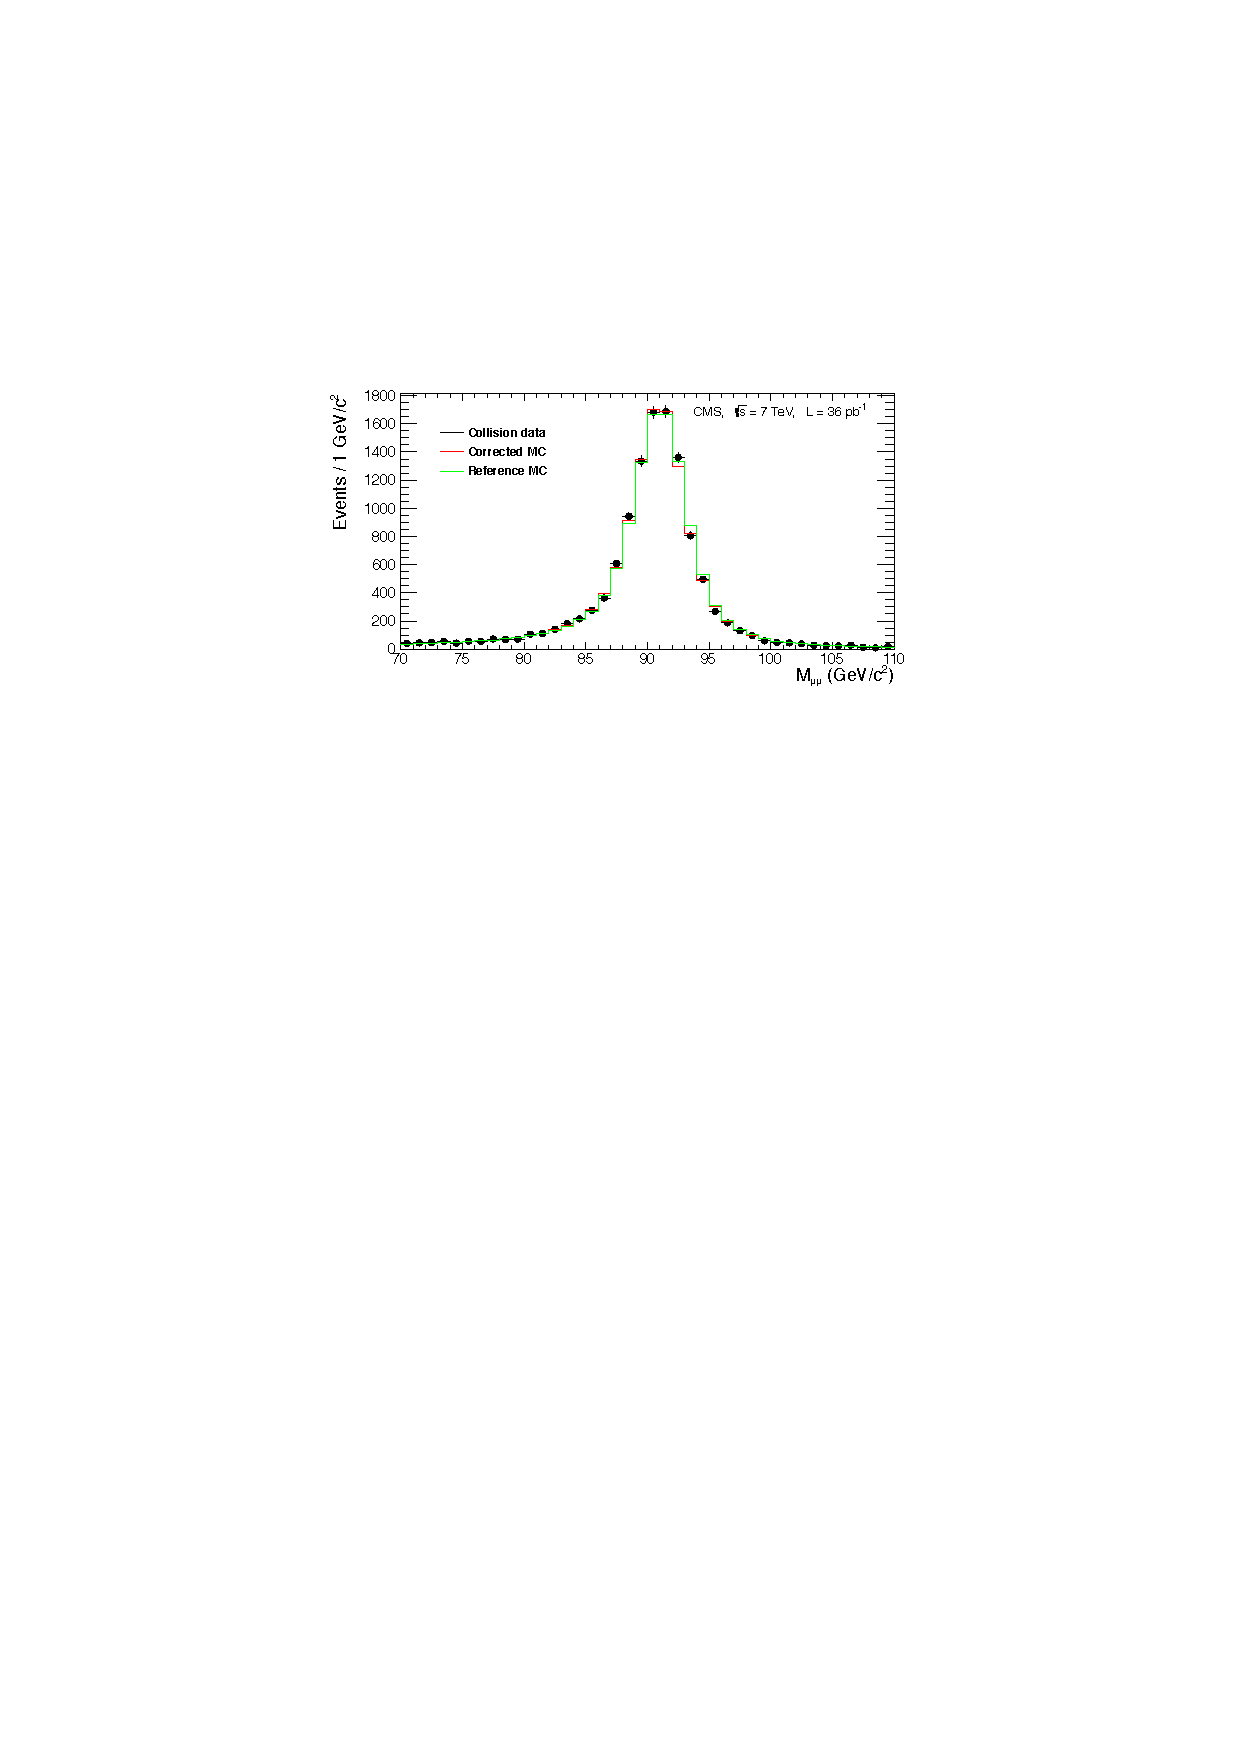
\includegraphics[width=.7\textwidth]{figures/muon_Z_resolution.pdf}
      \caption{Data and simulation of Z to di-muon events at 7 TeV. The black dots represent data from the detector, while the green line-shape represents the expected line shape for Z$\to\mu\mu$ events using the baseline detector simulation. Corrections are derived from this data and propigated forward Taken from \cite{cms_muons}.}
      \label{fig:muon_Z_resolution}
    \end{figure}
    
  \subsection{Photon Measurement Pipeline}
    ECAL measurements, lepton conversions. Photons probably pair produce in higher eta ranges, how does that work?
    \todo{plot for photon energy resolution?}
  \subsection{Jets} \label{sec:jets}
    Describe charged hadron subtraction, JECs ~\cite{JERC}, \cite{JEC_2016}
    pfCHSjets with L1FastL2L3 corrections (MC), L1FastL2L3L2L3residual corrections (data).
    \verb=Summer16_23Sep2016V3= JEC payload used to correct jets
    Need to put in blurbs about L1 Pile Up Corrections, L2L3 MC-Truth Corrections, and L2L3Residual Corrections (data only). Short descriptions here: https://twiki.cern.ch/twiki/bin/view/CMS/IntroToJEC 

    pfjetID

    Good info in Vince's Thesis and here: https://arxiv.org/pdf/1607.03663.pdf
    Roughly: L1 -- (pileup offset correction) pileup correction use QCD MC to get avg energy change to jet with and without pileup overlay. Look in 2D plane of $\eta$ and \pt, get correction.
    L2L3 -- (simulated response correction) Look at dijet events in MC, see how energy reco is different across \pt and $\eta$, correct for it.
    L2L3 Residual -- (Residual Corrections for data) Make MET 0 in dijet/ZJet/GammaJet events.

    jet energy mismeasurements are a function of the absolute scale of energy

    \todo{plot for jet energy resolution?}
  \subsection{B-Tagging} \label{sec:b-tagging}
    What is B-tagging? What do they look at? What's the false positive rate that we use?

  \subsection{MET Reconstruction} \label{sec:MET_reco}
    Make sure to add bits about sources of MET and the Type 1 correction
  \subsection{MET Filters} \label{sec:met_filters} 
    We apply certain filters that kill events, these are called MET filters but include things like beam halo as well.

\section{Monte Carlo} \label{sec:monte_carlo}
  Physics generated using Madgraph 5 interfaced with pythia8 for showering. List samples and their generator.
  SUSY models are also simulated using the madgraph package, but are then passed through the fastsim toolkit \cite{fastsim} rather than the full GEANT simulation. Statistical uncertainty in MC.
  \subsection{Summary of Simulated Samples} \label{sec:summary_of_simulated_samples}
    
    In this section we list all the Monte Carlo (MC) samples used for this analysis as well their generator and detector simulation.

    In this section we list the MC samples used for the \pt reweighting closure test.
      \begin{table}[htb]
        \begin{center}
          \scriptsize
          \caption{\label{tab:closuremc} List of MC samples used for the closure test.}
          \begin{tabular}{l|l|c}  
            \hline
            \hline
            Process & Dataset Name                                                            & Cross Section [pb]\\
            \hline
            \gjets   & \verb=/GJets_DR-0p4_HT-40To100_TuneCUETP8M1_13TeV-*-v1=                & 18560    \\
                     & \verb=/GJets_DR-0p4_HT-100To200_TuneCUETP8M1_13TeV-*-v1=               &  5000    \\
                     & \verb=/GJets_DR-0p4_HT-200To400_TuneCUETP8M1_13TeV-*-v1=               &  1079    \\
                     & \verb=/GJets_DR-0p4_HT-400To600_TuneCUETP8M1_13TeV-*-v1=               &   125.9  \\
                     & \verb=/GJets_DR-0p4_HT-600ToInf_TuneCUETP8M1_13TeV-*-v1=               &    43.36 \\
            \hline   
            \zjets   & \verb=/DYJetsToLL_M-50_TuneCUETP8M1_13TeV-*_ext1-v2=                     &  6021    \\
                     & \verb=/DYJetsToLL_M-50_HT-100to200_TuneCUETP8M1_13TeV-*_ext1-v1= &   181.3   \\
                     & \verb=/DYJetsToLL_M-50_HT-200to400_TuneCUETP8M1_13TeV-*_ext1-v1= &    50.42  \\
                     & \verb=/DYJetsToLL_M-50_HT-400to600_TuneCUETP8M1_13TeV-*_ext1-v1= &     6.984 \\
                     & \verb=/DYJetsToLL_M-50_HT-600to800_TuneCUETP8M1_13TeV-*-v2= &     1.681 \\
                     & \verb=/DYJetsToLL_M-50_HT-800to1200_TuneCUETP8M1_13TeV-*-v1= &    0.7754  \\
                     & \verb=/DYJetsToLL_M-50_HT-1200to2500_TuneCUETP8M1_13TeV-*-v1= &   0.1862  \\
                     & \verb=/DYJetsToLL_M-50_HT-2500toInf_TuneCUETP8M1_13TeV-*-v1= &    0.004385  \\
            \hline
            Campaign & \verb=*madgraphMLM-pythia8/RunIISummer16MiniAODv2=                       & \\
                     & \verb=-PUMoriond17_80X_mcRun2_asymptotic_2016_TrancheIV_v6*/MINIAODSIM= & \\

            \hline
            \hline
          \end{tabular}
          \end{center}
      \end{table}

\section{Datasets} \label{sec:datasets}
We use dilepton trigger events, as will be described in section \ref{sec:leptonic_final_states}
  \chapter{A search for new physics in events with a Z boson, missing transverse energy, and jets}

\section{Motivations}

  This search for new physics is motivated by observations of dark matter in astrophysical and cosmological data as well as the hierarchy problem. Supersymmetry provides a solution to these two problems at once in theories with `R-parity' conservation due to the existence of a lightest supersymmetric particle (LSP) which can not decay to standard model particles. If the LSP is not charged, then it is a natural candidate for dark matter. 

  The hard part of searching for dark matter is that it is known to not interact via the strong or electromagnetic forces with any non-trivial cross section. Therefore, the only signature dark particles will leave in a detector like CMS is transverse momentum imbalance, which is the central variable we use in this search.

  \subsection{Motivating Models} \label{sec:susy_models}

  We use several simplified SUSY models to motivate our search regions and interpret our results. Feynman diagrams of the additional operators in these models are shown in figures \ref{fig:feynman_str} and \ref{fig:feynman_ewk}. In each model, one or more of the new particle masses are free parameters. Setting maximal masses for these particles that are compatible with our observations is the intent of this style of SUSY search. These models are simulated with different values for the free mass parameters using the madgraph package as discussed in sec. \ref{sec:summary_of_simulated_samples}. A scan is then done over the simulated mass points to check whether the expected signature for any mass point describes the data better than the background only hypothesis, this is the content of section \ref{sec:exclusion_limits}.

  In fig. \ref{fig:feynman_str} we have a model of gauge mediated SUSY breaking (GMSB) where the LSP is a gravitino and is assumed to have the arbitrary low mass of 1 GeV. The gluino and neutralino masses are free parameters. We refer to this model as ``strong SUSY" because two gluinos are produced which cause the initial cascade of particles. The production of gluinos in this model tends to lead to many hadronic jets in the final state. The ``strong signal regions", defined in sec \ref{sec:search_regions}, are built to target this model.

  In fig. \ref{fig:feynman_ewk}, we have three models which we refer to as ``electroweak SUSY". In these models, electroweak superpartners are created in the collision without associated jets. The free parameters in these models are the masses of the electroweak superpartners. Due to the different branching ratios for Higgs and W/Z decays, two different signal regions are defined to target the left two diagrams (the VZ region) and right diagram (the HZ region). In models with a gravitino, it is again assumed to have a mass of 1 GeV.

  \begin{figure}[h!]
    \centering
    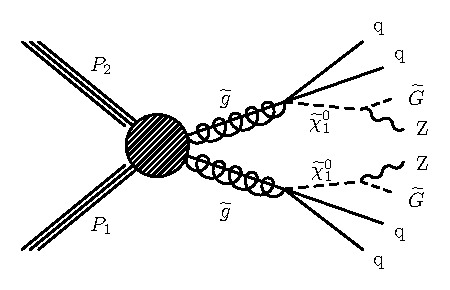
\includegraphics[width=.5\textwidth]{figures/diagrams/T5ZZ.pdf}
    \caption{The Feynman diagram for the additional term added to The Standard Model lagrangian to produce the simplified supersymmetric model used to interpret this in analysis in the context of ``strong SUSY". In this model of GSMB, the gravitino is the LSP with an assumed mass of 1 GeV. Two gluinos are produced in the collision which decay to neutral electroweak superpartners that couple to the Z boson. Because the model assumes the production of gluinos, large amounts of hadronic activity is expected.}
    \label{fig:feynman_str}
  \end{figure}

  \begin{figure}
    \begin{center}
      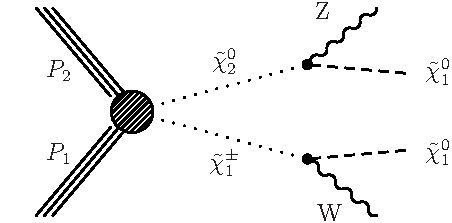
\includegraphics[width=0.3\textwidth]{figures/diagrams/TChiWZ.pdf} 
      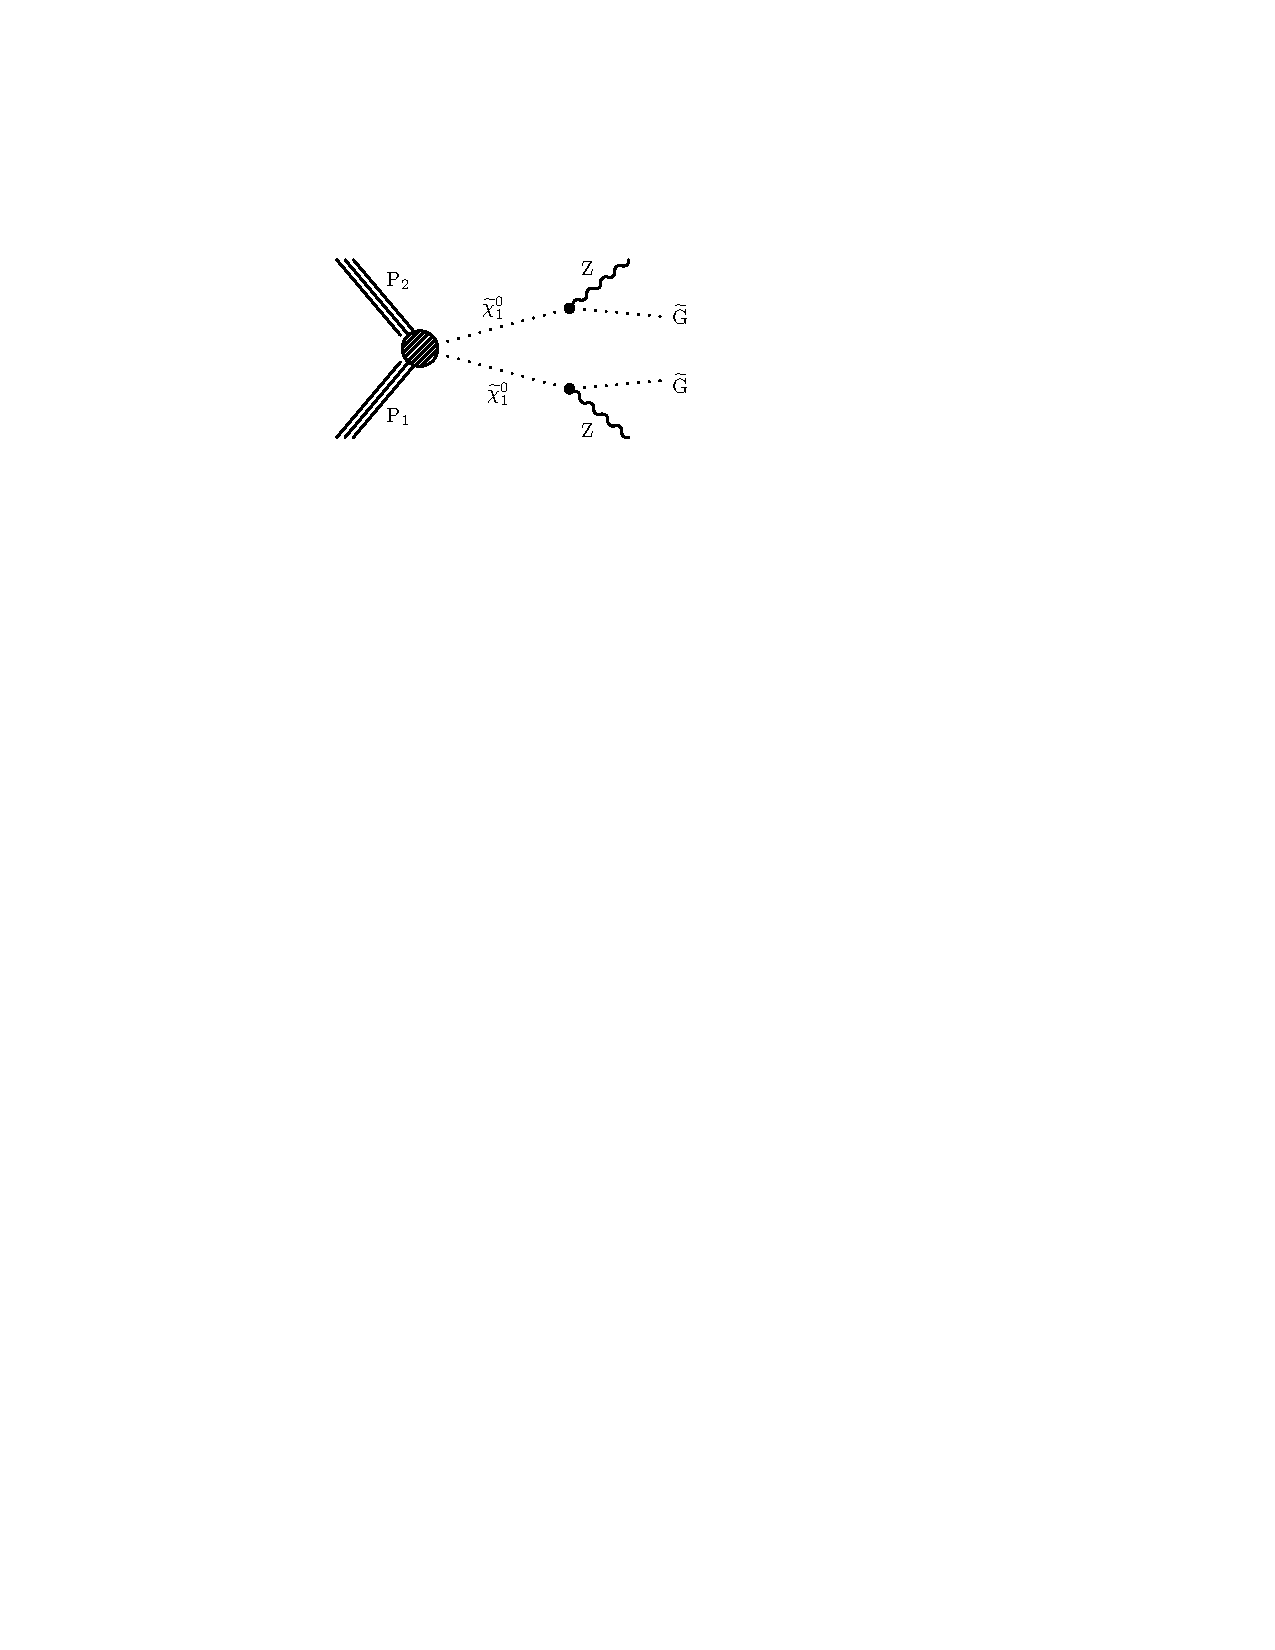
\includegraphics[width=0.3\textwidth]{figures/diagrams/TChiZZ.pdf} 
      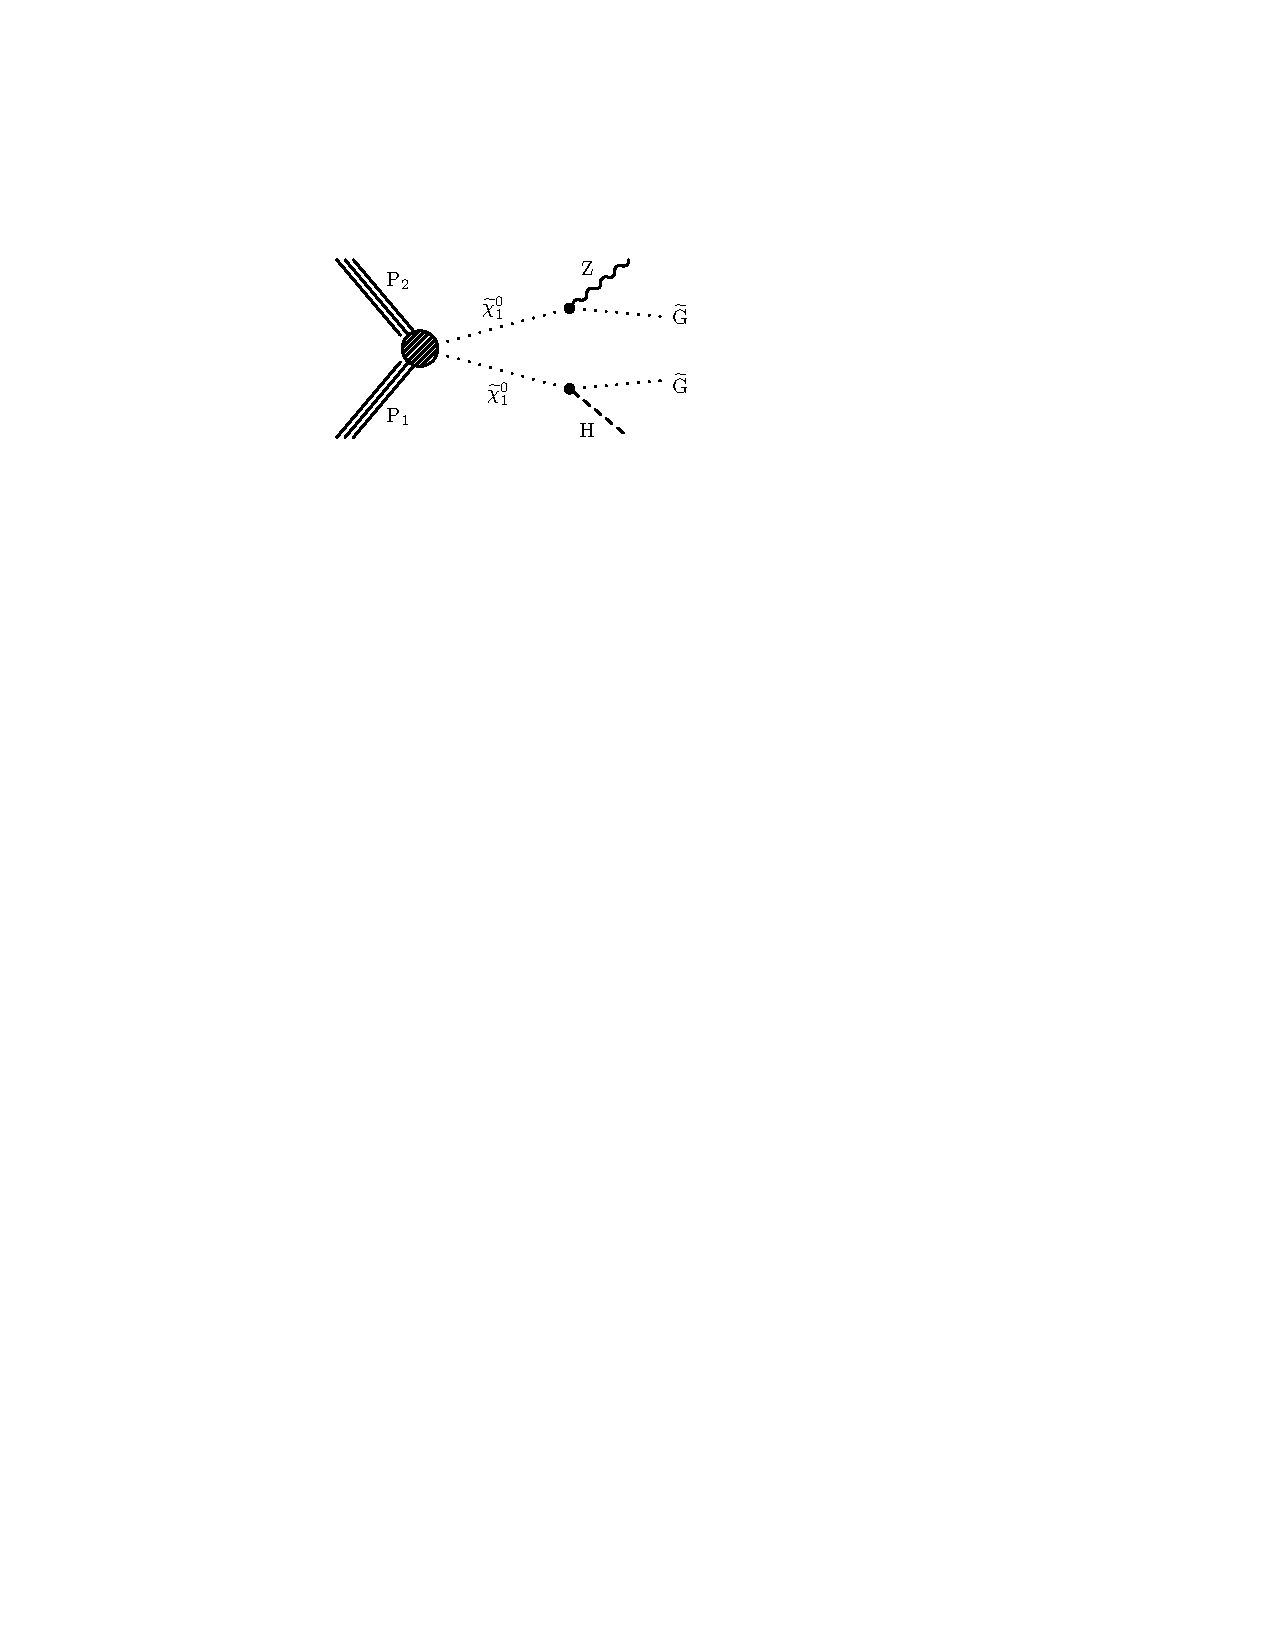
\includegraphics[width=0.3\textwidth]{figures/diagrams/TChiHZ.pdf} 
    \end{center}
    \caption{
      \label{fig:feynman_ewk} The Feynman diagrams for the electroweak SUSY models. In each diagram, electroweak superpartners are created in the collision and decay to either electroweak or Higgs bosons. The right two models again represent GMSB with a gravitino that is assigned a mass of 1 GeV.
    }
  \end{figure}

  \clearpage

\section{Analysis Strategy}

  \subsection{Background Considerations} \label{sec:background_considerations}

    \subsubsection{Leptonic Final States} \label{sec:leptonic_final_states}
      The Z boson can decay to any fermion. In theory, one could perform this analysis in an all hadronic final state, which might seem advantageous as the Z will decay to hadrons approximately 10 times as often as it will decay to light leptons.\cite{PDG} However, there are several reasons leptonic final states are highly advantageous.

      In hadron colliders, the most common types of final states are those with only hadronic activity, as can be seen in figure \ref{fig:lhc_decay_modes}; leptonic final states provide a much cleaner population in which to search for Z bosons. Additionally, as referenced in \ref{sec:electron_measurement_pipeline}, \ref{sec:muon_measurement_pipeline}, and \ref{sec:MET_reco}, the fidelity of energy measurements for the light leptons is much better than for jets at CMS. This provides great advantage for background discrimination; leptons from Z boson decays will tend to have a very specific dilepton mass, a quantity reconstructed from the momentum measurements.

      The decays of the Z produce two opposite sign, same flavor fermions. A further benefit of the leptonic channel is that flavor and charge identification is fairly easy for the light leptons but nearly impossible to identify for jets at the current state of the art (for instance, one can not say with high confidence that a jet was produced by a positively charged charm quark).

      Therefore, even though the branching ratio to light leptons from Z bosons is lower than the branching ratio to hadronic final states, the better energy resolution, lower background rates, and flavor identification make the leptonic final states far more powerful.

    \subsubsection{Background Sources}
      When using the leptonic final states, there are essentially two other background sources of leptons we must consider, these are $\gamma$ and W decays. Due to the high mass of the Z boson, any $\gamma \to \ell^\pm \ell^\mp$ events can easily be vetoed since these events should have dilepton mass peaking at 0 GeV. 

      The W boson will decay into leptons only with their complimentary neutrino, this means that in order to select a pair of opposite charge and same flavor charged light leptons, there must be at least two W bosons in the event. Because the decays of the W will be independent, there is only a 50\% chance that the two leptons will have the same flavor. As will be discussed later, this makes the background prediction for these types of events straightforward as events with two different flavor leptons can be used to model essentially any kinematical distribution.

      It turns out the most common source of W bosons is through the production of two top quarks which decay to a bottom quark and a W boson. To reject these events, we will use the MT2 variable, described in sec \ref{sec:b-tagging}. Further, the dilepton mass in $t\bar{t}$ events will be distributed essentially flatly across the Z mass window. The overall dilepton mass distribution will be a falling distribution with a small bump for the Z Boson. 

      Finally, due to the instability of the $\tau$ lepton, we neglect this channel from the search. $\tau$ leptons are much harder to identify than the light leptons, and further they can decay to light leptons in a flavor symmetric manner, so are predicted by that background channel's prediction method.

    \subsubsection{Hadronic Activity Requirements}
      As mentioned above, the major production mode of opposite sign dilepton pairs with dilepton mass near 91 GeV is from Drell-Yan production of Z bosons. The diagram for this type of process is shown in fig. \ref{fig:DY-diagram}. As can be seen in the figure, the leading order diagram for this process has no free quarks or gluons. That there are no free colored particles means that the vast majority of these events will likewise come without any jets. 

      \begin{figure}[h!]
        \centering
        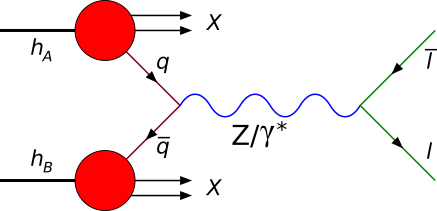
\includegraphics[width=.5\textwidth]{figures/Drell-Yan_feynman_edit.png}
        \caption{A diagram showing the Drell-Yan process. A quark and an anti-quark annihilate into an off-shell $\gamma$ or Z boson, which in turn decays to a pair of opposite-charge same-flavor leptons.}
        \label{fig:DY-diagram}
      \end{figure}

      Higher order diagrams with ISR or FSR take a cross-section production hit of roughly 1/5 due to the additional factor of the QCD coupling, $\alpha_s$, in the phase space integral. This means that we can suppress the DY background by a factor of almost 100 by requiring at least 2 jets in an event. This requirement is adopted in all search regions to keep our Drell-Yan background count low. Further, the background prediction for 0 or 1 jet events would require a completely different methodology due to different sources of \MET in high jet multiplicity final states. Therefore, this analysis limits itself to final states with at least 2 jets. 

      \begin{figure}[h!]
        \centering
        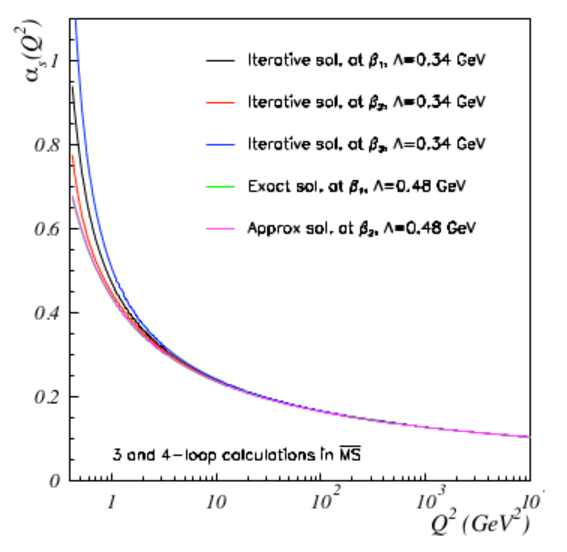
\includegraphics[width=.5\textwidth]{figures/QCD_Coupling_Running.pdf}
        \caption{The QCD coupling constant computed to different orders and different cutoff scales. The production of the Z boson is much more likely at center of mass energy near the mass of the Z. This means that $\alpha_s$ is between $\frac{1}{5}$ and $\frac{1}{10}$, which can be viewed as the zeroth order multiplicative correction to the DY with a single ISR or FSR jet cross section} 
        \label{fig:alpha_s_running}
      \end{figure}

      In addition, the strong SUSY model shown in fig. \ref{fig:feynman_str} anticipates lots of hadronic activity. Therefore, in the strong search regions, we also bin in the number of jets\footnote{This has the added benefit of creating search regions which are dominated by only one of the two dominant backgrounds, $t\bar{t}$ and Drell-Yan.} and require considerable hadronic activity by selecting events with $H_T$\footnote{$H_T$ is the scalar sum of transverse energy for all jets in an event, above certain thresholds.} above 200 or 500 GeV for the regions with and without b-tags respectively. This further rejects Drell-Yan events.


    \subsubsection{\MET Binning}

      Dark particles are expected to leave no signature in the detector except transverse momentum imbalance. In order to get maximal sensitivity to the different mass points for the SUSY models, we bin the search regions in \MET.

    \subsubsection{B-Tagging} \label{sec:b-tagging}
      We bin search regions in number of b-tags, which are outlined in detail in sec \ref{sec:b-tagging}. For the region targeting the HZ model, this is because the Higgs primarily decays to a pair of b-quarks. For the VZ model, we require there be no b-tags as it suppresses the $t\bar{t}$ background. For the strong search regions, we separate regions based on whether they have any b-tags, this because it causes the background composition to change dramatically; in regions with a b-tag, the dominant background will be $t\bar{t}$, whereas in regions without any b-tags the dominant background will be Z+jets. In turn, this allows us to use a slightly more aggressive MT2 cut in regions with a b-tag.

    \subsubsection{MT2} \label{sec:MT2}
      The MT2 variable is defined as

      \[
      \text{MT2} = \min \limits_{\text{\MET splittings}} \left[ \max \left\{ \MT(p_1, \slashed{p}_1), \MT(p_2, \slashed{p}_2) \right\} \right]
      \]

      where $\slashed{p}_1$ and $\slashed{p}_2$ are decompositions of the \MET vector, and M$_{\text{T}}$ is the transverse mass. 

      \begin{figure}[h!]
        \centering
        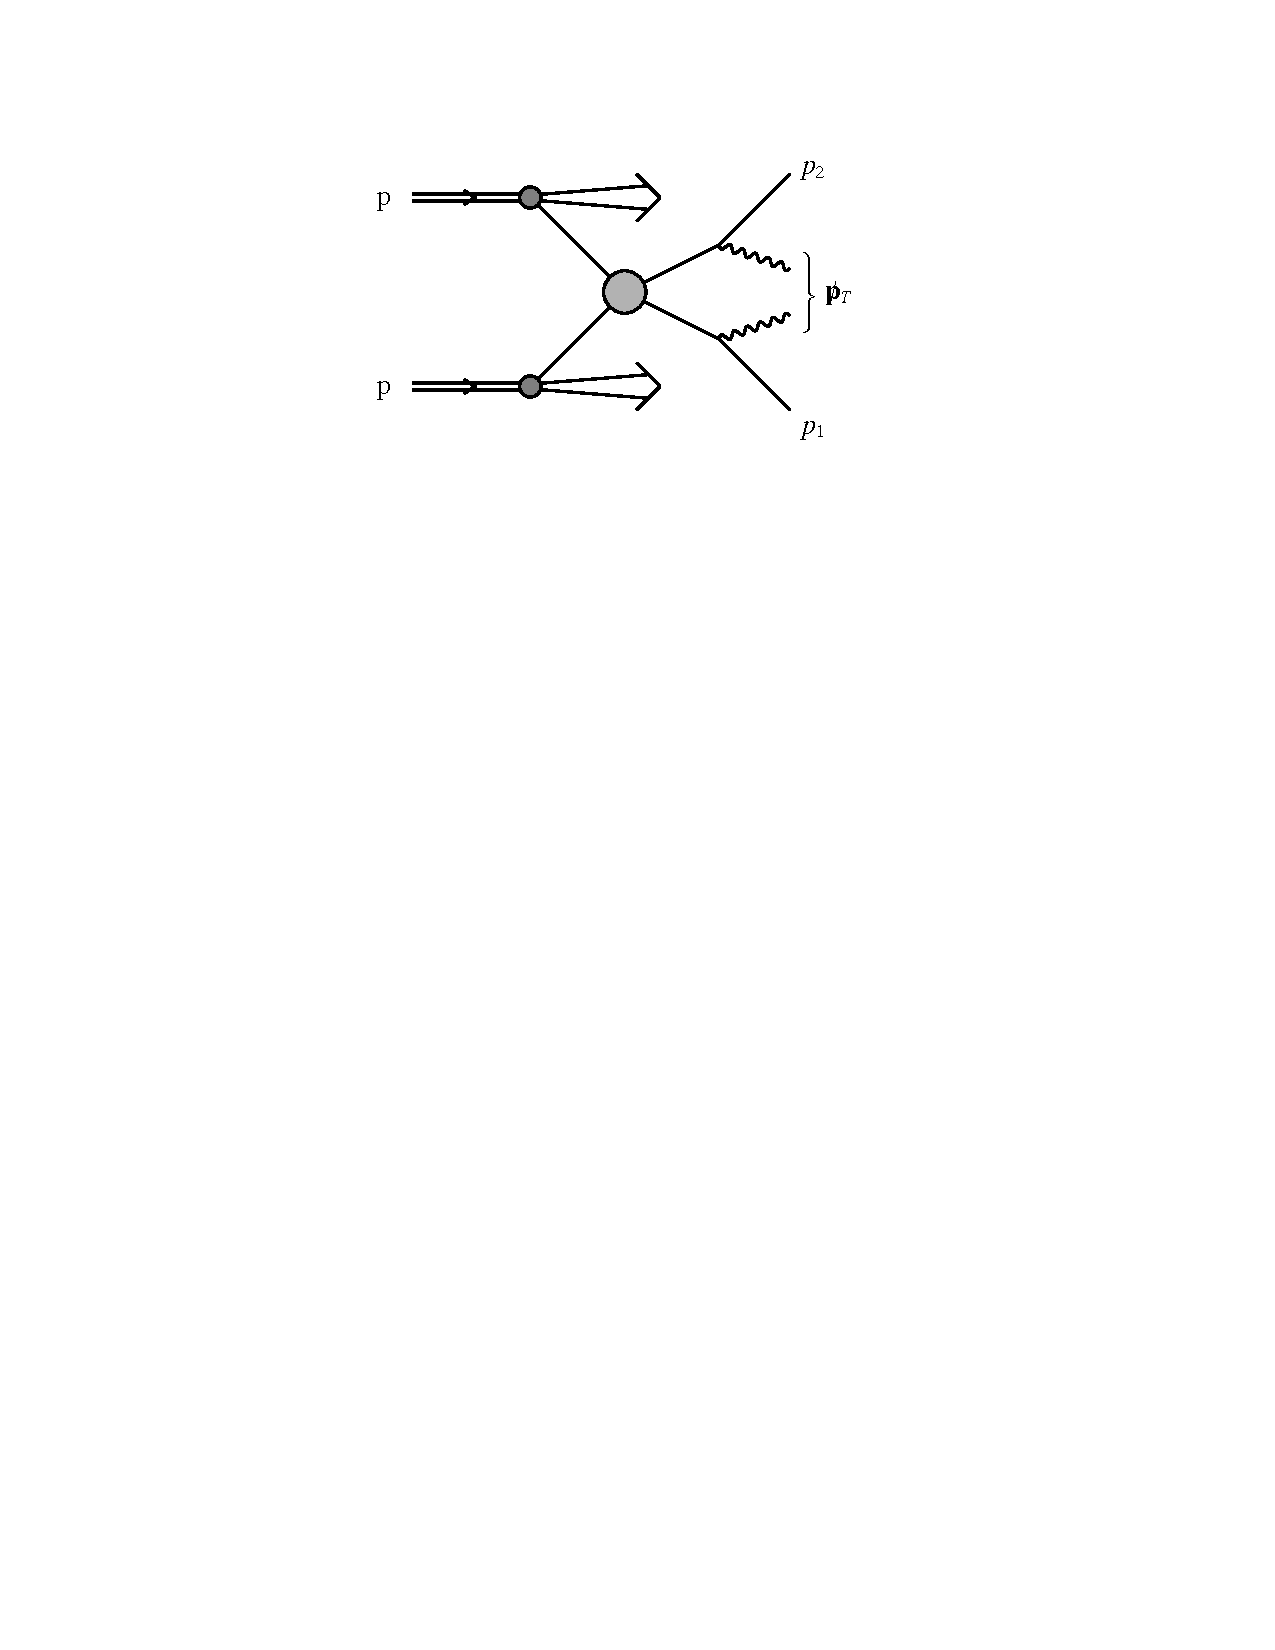
\includegraphics[width=.5\textwidth]{figures/mt2_diagram.pdf}
        \caption{The canonical picture of a decay with an MT2 endpoint, taken from the original paper\cite{mt2_paper}. }
        \label{fig:MT2_feynman_diagram}
      \end{figure}

      When a pair of W bosons each decay into a lepton and a neutrino, this value should not be able to be larger than the mass of the W boson. We can see this is true because for the correct splitting of the \MET vector into the momenta of the two neutrinos, the \MT for each lepton is bounded by the W mass. Therefore by summing over all possibilities, we will ensure the outer minimum will select at most the mass of the W (there is no lower limit besides 0). 

      However, in the case of an arbitrary decay, for instance in DY or in signal models with dark matter, there is no need for this value to be smaller than the mass of the W and generally higher values will be found. Therefore, we can use this quantity as a handle for rejecting events where the leptons come from two W bosons. We require in our strong search regions that MT2 be at least 80 GeV, just about the mass of the W boson. This mainly rejects the $t\bar{t}$ background. \todo{Why does any TTBar actually get through?}

    \subsubsection{MT2b}

      \begin{figure}[h!]
        \centering
        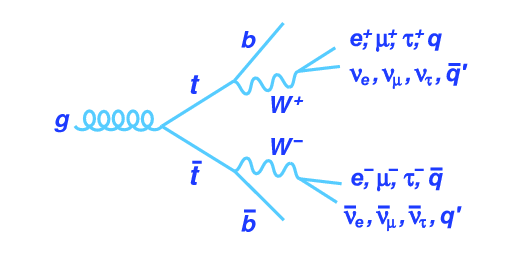
\includegraphics[width=.5\textwidth]{figures/ttbar_diagram.png}
        \caption{Diagram of $t\bar{t}$ production. An MT2-like endpoint can be found at the top mass if the lepton and b-quark momentum vectors are added so that choosing the \MET splitting that corresponds to the actual neutrino momenta will recover the transverse 4-vector of the top at the root of the decay. Figure taken from \cite{TTBar_figure}.}
        \label{fig:ttbar_diagram}
      \end{figure}

      Another variable used in this analysis is MT2b, or sometimes MT2($\ell b \ell b$), which can only be computed in events with 2 jets that are b-tagged. MT2 can be computed for any pair of 4-vectors along with a \MET vector. In the case of $t\bar{t}$ decays, shown in figure \ref{fig:ttbar_diagram}, one can see that by summing the 4-vectors for the lepton and b-quark, an MT2 end point should be found at the top mass, so long as the correct b-quark can be associated with the correct lepton. 

      The same power of MT2 to reject semi-invisibly decaying pair produced particles can be used to reject $t\bar{t}$ events in a population with 2 b-jets by trying the two different combinations of b-jet/lepton pairing and selecting the minimum value out of those two. Again, in the case of $t\bar{t}$ decay, MT2b defined in this way will have the mass of the top quark as one of the possible combinations, whilst there is no such requirement for a general process. MT2b is used only in the electroweak VZ region.

\section{Object Selection}

  \todo{Add all the variables in this section to the glossary? Which do I need to explicitly define?}

  After the particle flow algorithm identifies lepton, jet, and photon candidates, and before events can be classified as belonging to the various search, control, and closure regions, an additional set of selections are applied in order to further purify the analysis object collection. The purpose of this section is to define these selections.

  \subsection{Lepton ID} \label{sec:lepton_id}
    There are essentially two ways to get ``fake" leptons in the particle-flow lepton population:

    \begin{enumerate}
      \item A set of calorimeter and tracker hits from hadronic activity mimics the geometry expected by an lepton closely enough that a lepton is reconstructed from what should be called a jet.
      \item A colored particle, normally a charm or bottom quark, emits an electroweak boson that decays into a real lepton. In physics parlance, this is called \emph{non-prompt} lepton, as it is a secondary decay (\emph{prompt} meaning created at the primary vertex).
    \end{enumerate}

    Although item (2) is a ``real" lepton in the colloquial sense, in the context of most analyses, this one included, we do not want these sorts of objects contaminating our lepton population. To guard against these fake leptons, an additional set of cuts, called an ID, is required to be passed by each candidate before it is considered a ``good" lepton.

    In this analysis, we identify two ``working points" for leptons, tight and loose. These categories are defined based the lepton flavor and a set of cuts described below. Any lepton which passes the criteria to be classified as tight would necessarily pass the criteria to be classified as loose.

  \subsection{Lepton Isolation}
    In addition to the ID, isolation requirements are also necessary for leptons to be added to the analysis selection. In this analysis we use the variable miniRelIso, which is defined as the energy inside a variable size cone, determined by the lepton candidates \pt, about the lepton divided by the leptons \pt. The cone size is set by \pt in the following manner (units in \GeV):

    \[   
      \Delta R = 
      \begin{cases}
        0.2                & \pt < 50  \\
        \frac{10}{\pt}     & 50 \le \pt < 200 \\
        0.05               & \pt \ge 200 \\
      \end{cases}.
    \]

    The miniRelIso variable is then defined as the energy of all particle flow candidates inside the cone of size $\Delta R$ with effective area\footnote{See sec \ref{sec:jets}} corrections applied divided by the \pt of the lepton.

    \[
      \text{miniRelIso} = \frac{\text{E}_\text{cone}}{\pt}.\footnote{The miniRelIso variable is normally defined as just the energy of the cone, but for the sake of simplicity in terms of the use in this analysis, we define it as the ratio of the conventional miniRelIso to the lepton's \pt}
    \]

  \subsection{Electron ID and Isolation} \label{sec:electron_id_and_isolation}

    The electron candidates are required to pass the following cuts in addition to the particle flow identification:

    \begin{table}[!h]
      \begin{center}
      \caption{\label{table:electrons} Requirements for electron identification in addition to particle flow. Variables can be looked up in the \hyperref[ch:glossary]{Glossary} }
        \begin{tabular}{l|c}
          \hline
          Cut variable                  & Requirement   \\
          \hline
          \pt\                           & $>10$ GeV    \\ 
          $d_{0}$ (w.r.t. 1st good PV)   & $<0.05$ cm   \\
          $d_{z}$ (w.r.t. 1st good PV)   & $<0.1$  cm   \\
          miniRelIso                     & $<0.10$      \\
          abs(SIP3D)                     & $< 8$        \\
          maxLostHits                    & $==$ 0       \\
          Conversion Veto                & must pass    \\
          Spring 2016 POG MVA            & see below    \\
          miniRelIso                     & $<0.10$      \\
          \hline
        \end{tabular}
      \end{center}
    \end{table}

    The tight and loose criteria for electrons is based entirely on the MVA output. The POG MVA is a boosted decision tree (BDT)\footnote{A boosted decision tree is a sort of classifier that assigns a real number to a well-formed tuple of data. The algorithm tries to construct a map such that the number output for tuples in the same category are close to each other, then that number can be used discriminate between categories. Technical details are beyond the scope of this thesis, but a good review can be found \todo{find BDT document}. In the case of the electron ID MVA, the categories are real or fake and the numbers lie between -1 and 1.} prepared by the CMS EGamma Physics Object Group (POG). The BDT is trained on simulated Z$\to e^+ e^-$ events where electrons are considered to be real if the candidate can be matched to an electron emitted from the Z, and fake otherwise. An additional validation sample of mostly real electrons in data is constructed from $e^+ e^-$ events where the dilepton mass is within 7.5 GeV of the Z pole mass, $\abs{M_{ll} - M_Z} < 7.5$ GeV, and each lepton is required to be isolated such that the energy in a cone around the electron must be less than 10\% of the total energy in the cone (including the electron). A sample of mostly fake leptons in data is constructed by requiring a third lepton candidate in these events which has inverted isolation criteria and the additional requirement that the \MET in the event is less than 25 GeV to suppress WZ events. 

    Distributions of various kinematical quantities are constructed from simulation and data that have reason to discriminate between real and fake electrons, for instance the spread of the calorimeter hits in $\eta$. Some of these distributions are shown in figure \ref{fig:electron_mva_discriminating_vars}. The MVA is trained on the simulated events then checked against the data samples described above for consistency. Finally electrons in the barrel region and endcap regions are partitioned and each set is used to train an MVA specifically targeting the detector subsystems there \cite{Electron_reco}. 

    \begin{figure}[!h]
      \centering
      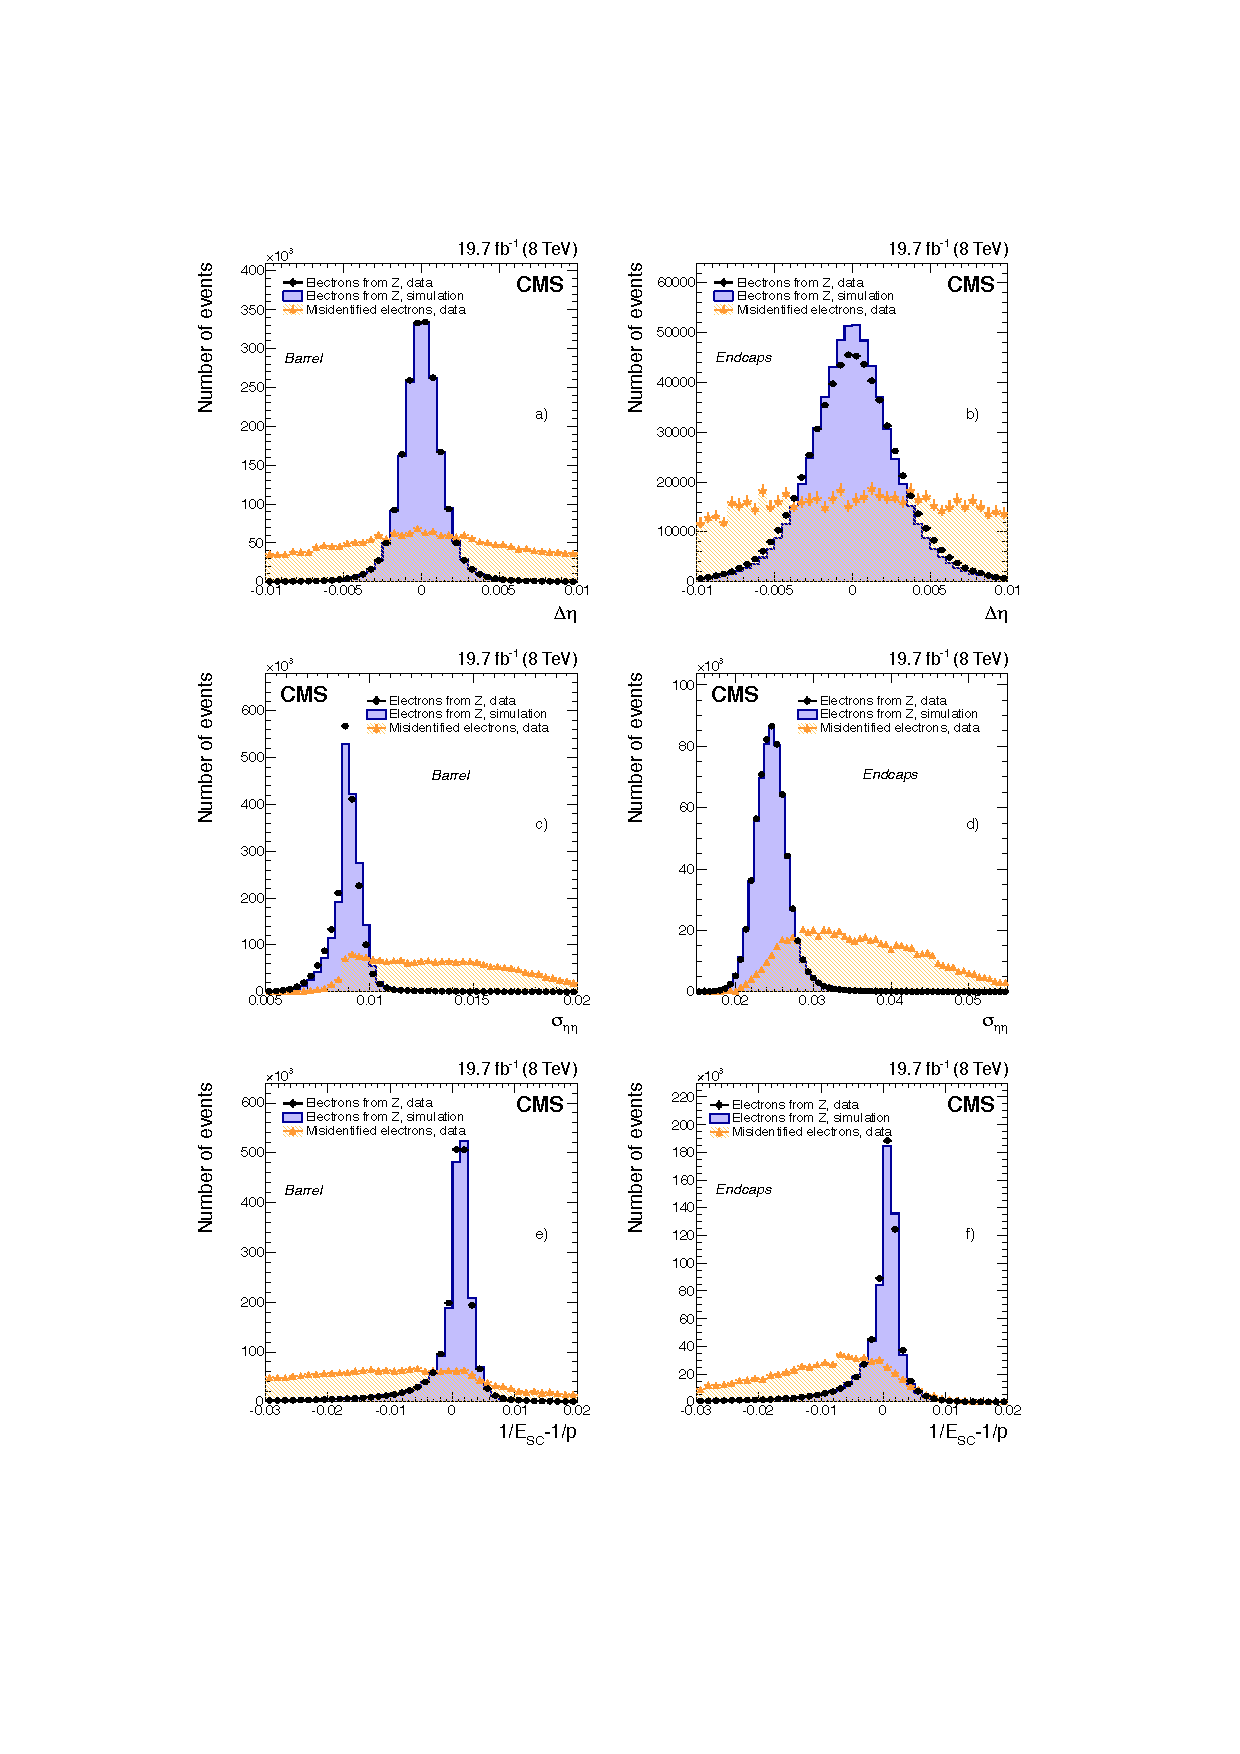
\includegraphics[width=.8\textwidth]{figures/electron_mva_discriminating_distributions.pdf}
      \caption{Some distributions used in the electron MVA that help discriminate between real (prompt) and fake (non-prompt) electrons. Simulation provides a guaranteed way to tag electrons as prompt or not-prompt, and so is used to train the MVA. However, it is important that data and simulation agree in these variables. $\Delta \eta$ and $\sigma_{\eta\eta}$ are variables that characterize the spread of detector hits associated with the electron in the $\eta$ direction. $E_\text{SC}$ is all the energy deposited into the ECAL which is associated to the electron, and $p$ is the electron's momentum. \todo{Do I need to make these plots myself?}}
      \label{fig:electron_mva_discriminating_vars}
    \end{figure}

    The working points for electrons based on the MVA output are shown below:

    \begin{table}[!h]
      \begin{center}
        \caption{\label{tab:elId}  Electron identification working points used in this analysis.}
        \begin{tabular}{rl|rl|l|l}
          \hline
          \multicolumn{2}{c|}{pseudorapidity region} & \multicolumn{2}{c|}{momentum [GeV]} & loose WP & tight WP \\ 
          \hline\hline
          $0<~|\eta|$&$<0.8$     &  10 $<$ ~\pt\ &$<$ 15 &  -0.86 & 0.77 \\ 
          $0<~|\eta|$&$<0.8$     &  15 $<$ ~\pt\ &$<$ 25 &  -0.96+$0.10*\frac{\pt-15}{10}$ & 0.52+$0.25*\frac{\pt-15}{10}$ \\ 
          $0<~|\eta|$&$<0.8$     &   ~\pt\ &$>$ 25       &  -0.96 & 0.52 \\ 
          \hline
          $0.8<~|\eta|$&$<1.479$ &  10 $<$ ~\pt\ &$<$ 15 &  -0.85 & 0.56 \\ 
          $0.8<~|\eta|$&$<1.479$ &  15 $<$ ~\pt\ &$<$ 25 &  -0.96+$0.11*\frac{\pt-15}{10}$ & 0.11+$0.45*\frac{\pt-15}{10}$ \\ 
          $0.8<~|\eta|$&$<1.479$ &   ~\pt\ &$>$ 25       &  -0.96 & 0.11 \\ 
          \hline
          $1.479<~|\eta|$&$<2.5$ &  10 $<$ ~\pt\ &$<$ 15 &  -0.81 & 0.48 \\ 
          $1.479<~|\eta|$&$<2.5$ &  15 $<$ ~\pt\ &$<$ 25 &  -0.95+$0.14*\frac{\pt-15}{10}$ & -0.01+$0.49*\frac{\pt-15}{10}$ \\ 
          $1.479<~|\eta|$&$<2.5$ &  ~\pt\ &$>$ 25        &  -0.95 & -0.01 \\ 
          \hline\hline
        \end{tabular}
        
      \end{center}
    \end{table}

    \clearpage

  \subsection{Muon ID and Isolation} \label{sec:muon_id_and_isolation}

    The muon ID is based purely on a cut-based approach, no MVA is used. Again, the selection criteria is based upon the muon POG, which is documented in more detail at ~\cite{muon_POG}. The selection used for the muon ID and isolation are defined below:

    \begin{table}[!h]
      \begin{center}
        \caption{\label{table:muons} Summary of the muons selection requirements. }
        \begin{tabular}{l|c|c}
          \hline
          \hline
          \multicolumn{3}{c}{Good Muon Requirements} \\
          \hline
          Quantity   &  Tight Requirement & Loose Requirement \\
          \hline
          Quality Muon                      & Must pass   & Must pass     \\
          Fraction of valid tracker hits    & $>$ 0.8     & $>$ 0.8  \\ 
          \hline
          $d_{0}$ (w.r.t. 1st good PV)   & $<0.05$ cm & $<0.05$ cm \\
          $d_{z}$ (w.r.t. 1st good PV)   & $<0.1$ cm  & $<0.1$ cm  \\
          SIP3D                          & $< 8$      & $< 8$      \\
          miniRelIso                     & $<0.20$    & $<0.40$       \\
          \hline
        \end{tabular}
      \end{center}
    \end{table}

    The criteria to be a ``Quality Muon" is given below:
    \begin{table}[!h]
      \begin{center}
        \caption{\label{table:muons} Summary of Quality Muon requirements.}
        \begin{tabular}{l|c}
          \hline
          \hline
          \multicolumn{2}{c}{Quality Muon Requirements} \\
          \hline
          Quantity   &  Requirement \\
          \hline
          Segment compatibility             &$>$ 0.451 \\
          \hline
          \emph{or} & \\
          \hline
          Normalized global-track $\chi^2$  & $<$ 3    \\
          Tracker-Standalone position match & $<$ 12   \\
          Kick finder                       & $<$ 20   \\
          Segment compatibility             & $>$ 0.303 \\
          \hline
          \hline
        \end{tabular}
      \end{center}
    \end{table}

    \todo{brief blurb on global/tracker muons.}

  \newpage

  \subsection{Photon Selection} \label{sec:photon_selection}

    Photons are used in this analysis as part of the Z+Hadronic background prediction. The details of this prediction are in \ref{sec:z_+_hadronic}. The bulk of these selections are in order to ensure there is no inefficiency for the trigger for $\gamma +$jets events. \todo{Rewrite the following list which was taken from the AN (written by Dom)}

    \begin{itemize}
      \item \pt $ > 25$ GeV
      \item $|\eta| < 2.4$
      \item No matching pixel track (pixel veto)
      \item There must be a jet candidate of \pt $ >$ 10 GeV matched to the photon within $\DR < 0.3$. 
      The matched jet is required to have a neutral electromagnetic energy fraction of at least 70\%.

      \item We reject photons which have an electron of at least \pt $>$ 10 GeV within $\DR < 0.2$
      in order to reject conversions from electrons from W decays which are accompanied by real \MET.

      \item We reject photons which are aligned with the \MET to within 0.4 radians in phi.
      \item To ensure full efficiency with respect to the isolated photon triggers used, we apply the following additional cuts:
      \begin{itemize}
        \item ratio of the energy of the energy of the photon's 3X3 supercluster to the photons 5X5 supercluster (R9) $>$ 0.92
        \item $\frac{H}{E} < 0.2$ %\fixme{is this the HLT H/E or still offline?}
        \item hollow track isolation $<$ 3 GeV
        \item photons with $|\eta| < 1.4$ have ECAL pfcluster iso $<$ 3 GeV + \pt ($\gamma$) * 0.0053
        \item photons with $|\eta| < 1.4$ have HCAL pfcluster iso $<$ 7 GeV + \pt ($\gamma$) * 0.014
        \item photons with $|\eta| > 1.6$ have ECAL pfcluster iso $<$ 3 GeV + \pt ($\gamma$) * 0.0034
        \item photons with $|\eta| > 1.6$ have HCAL pfcluster iso $<$ 7 GeV + \pt ($\gamma$) * 0.0139
      \end{itemize}
    \end{itemize}

    \todo{Maybe beef up this list with the full selections...}
    %\todo{Photon ID: https://github.com/cmstas/CORE/blob/master/OSSelections.cc#L360-L370}
    %\todo{Loose Selection: https://github.com/cmstas/CORE/blob/master/PhotonSelections.cc#L308-L342}
    %\todo{Template Photon: https://github.com/cmstas/CORE/blob/master/PhotonSelections.cc#L186-L192}
    %\todo{Trigger Emulation: https://github.com/cmstas/CORE/blob/master/PhotonSelections.cc#L420-L444}

  \subsection{Jet Selection} \label{sec:jet_selection}

  Jets are selected from the particle flow selection and are refined via ``charged hadron subtraction" and the Summer16\_23Sep2016V3 ``jet energy corrections" described in \ref{sec:jets}. In this analysis, we distinguish between jets and ``b-tagged jets." B-tagging is described in \ref{sec:b-tagging}, but it comes down to a numerical quantity assigned to each jet called its \emph{b-tag csv value}. If the csv value is large enough, a jet is considered likely to have been seeded by a bottom quark. 

      \begin{table}[!h]
      \begin{center}
        \caption{\label{table:muons} Summary Of Good Jet Requirements.}
        \begin{tabular}{l|c|c}
          \hline
          \hline
          \multicolumn{3}{c}{Jet Selections} \\
          \hline
          \hline
          Quantity                  & \multicolumn{2}{c}{ Cut Value } \\
          \hline
          $\abs{\eta}$              & \multicolumn{2}{c}{$< 2.4$}   \\
          Lepton Veto               & \multicolumn{2}{c}{Not within $\abs{\DR} < 0.4$ of a tight lepton} \\
          Photon Veto               & \multicolumn{2}{c}{Not within $\abs{\DR} < 0.4$ of a good photon } \\
          Neutral Hadron Fraction   & \multicolumn{2}{c}{ $< 0.99$} \\
          Neutral EM fraction       & \multicolumn{2}{c}{ $< 0.99$} \\
          Charged hadron fraction   & \multicolumn{2}{c}{ $> 0   $} \\
          Charged multiplicity      & \multicolumn{2}{c}{ $> 0   $} \\
          Charged EM fraction       & \multicolumn{2}{c}{ $< .99 $} \\
          Number of constituents    & \multicolumn{2}{c}{ $> 1   $} \\
          \hline
          \hline
          Quantity                  &  Jet Requirement & B-tagged Jet Requirement\\
          \hline
          \pt                       & $> 35\; \GeV $     & $> 25\; \GeV$   \\
          B-tag CSV                 & None             & $> 0.8484$    \\
          \hline
          \hline
        \end{tabular}
      \end{center}
    \end{table}

  \subsection{Isolated Tracks} \label{sec:isolated_tracks}
  In addition to vetoing events which have extra loose leptons, a typically more inclusive veto is applied to kill events which might have an extra prompt lepton based on the identification of an isolated charged object. 

  To distinguish these types of objects, we introduce the notion of ``track isolation," defined as the total energy of all the particle flow charged candidates that trace back to within $\abs{dz} < 0.1$ cm of the primary vertex within a cone of $\abs{\DR} <0.3$ about the lepton.\footnote{Notice that the miniRelIso we defined above was defined as a relative isolation, the energy in a cone divided by the \pt of the object in question, track isolation as defined here has units of energy.}

  There are two types of isolated tracks, those that are seeded by particle flow charged hadron candidates, and those that are seeded by particle flow electron or muon candidates. The criteria on top of the particle flow identification for these two sources are listed in the tables below:

  \begin{table}[!h]
      \begin{center}
        \caption{\label{table:muons} Summary Of Isolated Track Requirements.}
        \begin{tabular}{l|c|c}
          \hline
          \hline
          \multicolumn{3}{c}{Isolated Track Selections} \\
          \hline
          \hline
          Quantity                  &  Charged Hadronic Requirement & Light Lepton Requirement\\
          \hline
          \pt                       & $> 10\; \GeV $                & $> 5\; \GeV$           \\
          Vertex Association\footnote{PVTight means the particle was closer to the primary vertex than any other reconstructed vertex. PVUsedInFit means the particle was used to define the primary vertex. There are more details in the glossary.}     & PVTight or PVUsedInFit  & PVTight or PVUsedInFit \\ 
          Track Isolation           & $<8\; \GeV$                   & $<8\; \GeV$             \\
          Track Isolation / \pt     & $<0.2$                        & $<0.1$                  \\
          $\abs{dz}$                & $< 0.1$ cm                    & $< 0.1$ cm              \\
          \hline
          \hline
        \end{tabular}
      \end{center}
    \end{table}

\section{Event Selection}

  The selection of events can be broken into several stages. Though each of these regions will be expanded upon in the following sections, in broad strokes there 4 separate final states used to accomplish this analysis. These final states define the signal regions and 3 control regions used to conduct this search:

  \begin{description}
    \bitem{Search Regions (SR)} Events with two opposite charge and same flavor light leptons build our search regions, we have either a $e^+e^-$ or a $\mu^+ \mu^-$ pair in each event.
    \bitem{Flavor Symmetric Control Regions} Events with two opposite charge and different flavor light leptons build our flavor symmetric control region, we have either a $e^+\mu^-$ or a $\mu^+ e^-$ pair in each event. This region is used to predict the flavor symmetric background.
    \bitem{$\gamma$+Jets Control Region} Events with a single photon are used to construct the $\gamma$+jets control region used for the Z+jets background prediction. 
    \bitem{EWK Contamination Closure Region} Events with a photon and muon are used to check the modeling of the ``EWK contamination" in the \MET Templates prediction, described in section \ref{sec:ewk_subtraction}.
  \end{description}

  The CMS datasets which seed these events are described in \ref{sec:datasets}.
  
  \subsection{Dilepton Selection} \label{sec:dilepton_selection}

    The following are the requirements for events with two light leptons, i.e. for the search regions and for the flavor symmetric control regions.  

    Light lepton candidates are tagged by the particle flow algorithm described in section \ref{sec:particle_flow}. In addition to the list below, leptons must also pass preselection ID and isolation requirements which differ depending on their flavor, but are described in \ref{sec:electron_id_and_isolation} and \ref{sec:muon_id_and_isolation} above.

    \begin{itemize}
      \item The (sub)leading lepton in each event must have at least (20) 25 GeV of transverse momentum. These points were selected so that the event would be in the "trigger turn-on" described in \ref{sec:event_triggering}.
      \item The pseudorapidity for each lepton must be within the inner tracker's fiducial area, namely $\left|\eta\right| < 2.4$
      \item No lepton should be in the ``dead zone" described in section \ref{sec:fiducial_area}, this is in the range $1.4 < \left|\eta\right| < 1.6$
      \item For the search region, events must have exactly one pair of opposite charge same flavor (OCSF) light leptons, for the flavor symmetric control region events must have exactly one pair of opposite charge and different flavor (OCDF) light leptons.
      \item The mass constructed out of the sum of lepton vectors (dilepton mass) must be between 86 and 96 GeV.
      \item The transverse momentum of the dilepton system must be at least 25 GeV. This is in order to ensure parity with the $\gamma$ selections used in the Z+hadronic background prediction.
    \end{itemize}

  \subsection{Event Vetos} \label{sec:event_vetos}
    Events are typically vetoed\footnote{precise definitions of the regions will be given below} across all search, control, and closure regions if any of the following are true:

    \begin{description}
      \bitem{Isolated Track Veto} Events with an isolated track, defined in \ref{sec:isolated_tracks}.
      \bitem{\MET Filters} Events where any of the ``\MET Filters", described in section \ref{sec:met_filters}, are true.
      \bitem{Jet/\MET alignment} Events where the \MET is aligned with the leading or subleading jet in the $\phi$ direction up to 0.4. Events with $\abs{\Delta \phi(\text{jet}_{1,2},\MET)} < 0.4$ are not accepted. 
    \end{description}

    Dilepton events specifically, those within the SRs and flavor symmetric control regions, are vetoed under the following conditions:

      \begin{description}
        \bitem{Lepton Cone Isolation} The two tight leptons are within a cone of $\Delta R < 0.1$ of each other.
        \bitem{Extra Lepton Veto} There is an additional loose or tighter lepton in the event. In other words, event with three or more loose IDed leptons are vetoed. IDs are defined in \ref{sec:electron_id_and_isolation} and \ref{sec:muon_id_and_isolation}. 
      \end{description}


    \todo{For the signal regions, we select events with opposite charge and same flavor dilepton pairs, for the flavor-symmetric background prediction, we select events with same sign and same flavor dilepton pairs, for the \MET templates prediction, we select from single photon events which are seeded by an entirely different dataset.}

  \subsection{Search Regions} \label{sec:search_regions}
    The search is broken into two distinct branches based on the motivating models listed in sec \ref{sec:susy_models}. The strong and electroweak search regions are summarized in the table below:

    \begin{table}[htb]
      \begin{center}
        \caption{\label{tab:selections_sr} Summary of signal region selections. }
        \begin{tabular}{l|l|l|l|l|l}
          \hline
          \hline
          \multicolumn{6}{c}{{\bf Search selections}}  \\
          \hline                                          
          \hline                                          
          \multicolumn{6}{c}{{\bf Strong Search Regions}}  \\
          \hline                                         
          Region & \njets & \nb & \Ht & \mttwol & \MET binning \\
          \hline                                         
          SRA b-veto       & 2--3 & = 0 & $> 500$~GeV & $> 80$~GeV & [100,150,250,$\infty$] \\
          SRB b-veto       & 4--5 & = 0 & $> 500$~GeV & $> 80$~GeV & [100,150,250,$\infty$] \\
          SRC b-veto       & $\geq6$ & = 0 & - & $> 80$~GeV &  [100,150,$\infty$] \\
          SRA b-tag (SRAb) & 2--3 & $\geq 1$ & $> 200$~GeV & $> 100$~GeV & [100,150,250,$\infty$] \\
          SRB b-tag (SRBb) & 4--5 & $\geq 1$ & $> 200$~GeV & $> 100$~GeV & [100,150,250,$\infty$] \\
          SRC b-tag (SRCb) & $\geq6$ & $\geq 1$ & - & $> 100$~GeV &  [100,150,$\infty$] \\
          \hline
          Baseline  & $\geq2$ & - & - & $> 80$~GeV &  $> 100$~GeV \\
          \hline                                          
          \hline                                         
          \multicolumn{6}{c}{{\bf Electroweak Search Regions}}  \\
          \hline                                         
          Region & \njets & \nb & dijet mass & \mttwo & \MET binning \\
          \hline                                         
          VZ & $\geq2$ & = 0 & $\mjj < 110$~GeV & $\mttwol > 80$~GeV & [100,150,250,350,$\infty$] \\
          HZ & $\geq2$ & = 2 & $\mbb < 150$~GeV & $\mttwolb > 200$~GeV & [100,150,250,$\infty$]  \\
          \hline                                          
          \hline
        \end{tabular}
      \end{center}
    \end{table}

    \begin{table}[htb]
      \begin{center}
        \caption{\label{tab:search_region_additional_selections} 
          Additional selections for the search regions. 
        }
        \begin{tabular}{l|r}\hline
        Cut & Value \\
        \hline 
        \hline
        Leptons                       & $e^\pm e^\mp$ or $\mu^\pm \mu^\mp$ with \pt $> 25(20)$ GeV for the (sub)leading lepton \\
        Dilepton Selections           & All outlined in sec \ref{sec:dilepton_selection}    \\
        Vetoes                        & Extra lepton                                        \\
                                      & Isolated Track                                      \\
                                      & Lepton Cone                                         \\
                                      & \MET Filters                                        \\
                                      & Jet/\MET Alignment                                  \\
        \hline
        \hline
        \end{tabular}
      \end{center}
    \end{table} 

    In addition to these selections, all dilepton selections, outlined above in sec \ref{sec:dilepton_selection}, and extra lepton vetoes, outlined above in sec \ref{sec:event_vetos}, are applied.

  \subsection{Flavor Symmetric Control Region} \label{sec:flavor_symmetric_control_region}     
 
    A flavor symmetric control region in constructed for every search region by flipping the requirement for an OCSF dilepton pair to a OCDF dilepton pair and widening the dilepton mass window from $\pm5$ GeV about the Z pole mass to $>20$ GeV. Table \ref{tab:flavor_symmetric_control_regions} summarizes below: 

    \begin{table}[htb]
    \begin{center}
      \caption{\label{tab:flavor_symmetric_control_regions} 
        Summary of selections for the flavor symmetric control regions.
      }
      \begin{tabular}{l|r}\hline
      Cut & Value \\
      \hline 
      \hline
      Baseline                      & Start with search regions from tables \ref{tab:selections_sr} and \ref{tab:search_region_additional_selections}  \\
      Flavor Selection              & Flip same flavor requirement, i.e. select $e^\pm\mu^\mp$ pair \\
      Dilepton Mass                 & Extend range to $>20$ GeV \\
      \hline
      \hline
      \end{tabular}
    \end{center}
  \end{table} 

  \subsection{$\gamma$+Jets Control Region} \label{sec:met_templates_control_region}

    In order to do the Z+jets background prediction, $\gamma$+jets events must be chosen in kinematic regions that mimic the search regions. The photon events must pass precisely the cuts for the signal region, listed in sec \ref{sec:search_regions}, to be used in constructing the prediction for that region, the details of which are described in sec \ref{sec:z_+_hadronic}. In addition to these event level selections, the photons themselves must pass the criteria in ``Photon Selection", sec \ref{sec:photon_selection}.

    One caveat is the MT2 and MT2b variables. In order to construct these in events without leptons, we simulate the decay of a Z boson, with momentum equal to that of the leading photon in the event, to two leptons. Those leptons are then used to construct all MT2-like quantities for this analysis.\footnote{\todo{Should I mention bugs here? We had a bug where we forgot to do this with MT2b, instead all the photon events just passed this cut.}}

    \begin{table}[htb]
    \begin{center}
      \caption{\label{tab:flavor_symmetric_control_regions} 
        Summary of selections for the flavor symmetric control regions.
      }
      \begin{tabular}{l|r}\hline
      Cut & Value \\
      \hline 
      \hline
      Baseline                      & Start with search regions from tables \ref{tab:selections_sr} and \ref{tab:search_region_additional_selections}  \\
      Flavor Selection              & Flip same flavor requirement, i.e. select $e^\pm\mu^\mp$ pair \\
      Dilepton Mass                 & Extend range to $>20$ GeV \\
      \hline
      \hline
      \end{tabular}
    \end{center}
  \end{table} 

  \subsection{EWK Subtraction Closure Region} \label{sec:ewk_subtraction_closure_region}

    The EWK Subtraction Closure Region is constructed to check the performance of physics simulation at predicting the \MET profile in W$\gamma$ events. The region is defined in table \ref{tab:ewk_sub_closure_region_definiton}.


    \begin{table}[htb]
      \begin{center}
        \caption{\label{tab:ewk_sub_closure_region_definiton} 
          Definition of the Electroweak Subtraction Closure Region
        }
        \begin{tabular}{l|r}\hline
        Cut & Value \\
        \hline 
        \hline
        $\mu$                         & Exactly one with \pt $> 25$ GeV   \\
        $\gamma$                      & At least one with \pt $> 25$ GeV  \\
        \MET                          & $> 50$ GeV                        \\
        \njets                        & $\ge$ 2                           \\
        $M_T(\mu, \MET)$              & $> 30$ GeV                        \\
        $\Delta \phi(\gamma, \MET)$   & $> 0.4$                           \\
        Vetoes                        & \MET filters                      \\
        \end{tabular}
      \end{center}
    \end{table} 

    Here $M_T(\mu, \MET)$ is the transverse mass\footnote{The mass of a 4-vector with the z-component set to 0.} of the $\mu$+\MET system. $\Delta \phi(\gamma, \MET)$ is the angle between the photon and the \MET vector in the x-y plane. 

  \subsection{\rsfof Measurement Region} \label{sec:rsfof_measurement_region}

    The \rsfof measurement region is defined in table \ref{tab:rsfof_measurement_region} 

    \begin{table}[h!]
      \begin{center}
        \caption{Definition of the \rsfof measurement region. \label{tab:rsfof_measurement_region} 
        }
        \begin{tabular}{l | r}\hline
        Cut       & Value   \\                          
        \hline 
        \hline
        Leptons   & Exactly 2 passing selections in sec. \ref{sec:dilepton_selection} on dilepton selection \\
        \MET      & $\in [100,150]$ GeV                 \\
        \njets    & $\ge$ 2                             \\
        \mll      & $\notin [70,110]$ GeV               \\
        Vetoes    & \MET filters                        \\
                  & Jet/\MET alignment                  \\
        \end{tabular}
      \end{center}
    \end{table}
    \FloatBarrier

  \subsection{$\kappa$ Measurement Regions} \label{sec:kappa_measurement_regions}

    The measurement of the $\kappa$ transfer factor is done in several regions. The baseline region, strong regions, HZ, and VZ, regions are defined in table \ref{tab:selections_sr}, for the measurement of $\kappa$ the same-flavor requirement is flipped to require $e\mu$ pairs in each event. The ``strong region with bs" is the sum of all strong search regions that have a b-tag, i.e. SRAb, SRBb, and SRCb, and ``strong region, b-veto" is the sum of strong search regions without a b-tag.

  \subsection{Z+$\nu$ Control Regions} \label{sec:znu_control_regions}

    These regions are used to normalize the MC samples used in the Z+$\nu$ background prediction. Three control regions are constructed for the three different processes. For all these regions, at least two leptons must pass the normal analysis selections listed in sec \ref{sec:dilepton_selection} on dilepton selections and in secs \ref{sec:electron_id_and_isolation} and \ref{sec:muon_id_and_isolation} on electron and muon ID and isolation respectively. Any 3rd or 4th leptons are required to pass the same ID requirements as well as requirements on the pseudorapidity, $\eta$, listed in sec \ref{sec:dilepton_selection} on dilepton selections. However, the isolation points are relaxed to \todo{ask Leonora} for electrons and \todo{ask Leonora} for muons.

    \begin{table}[htb]
      \begin{center}
        \scriptsize
        \caption{Definition of the WZ, ZZ, and TTZ control regions. These regions are used to normalize the MC in the Z+$\nu$ prediction. \label{tab:znu_control_regions_definitons} 
        }
        \begin{tabular}{l | r | r | r}\hline
        Cut       & WZ Value                             & ZZ Value                                &  TTZ Value                           \\
        \hline 
        \hline
        Leptons   & Exactly 3 with \pt $> 25,20,20$ GeV  & Exactly 4 with \pt $> 25,20,20,20$ GeV, & Exactly 3 with \pt $> 25,20,20$ GeV  \\
                  &                                      & second pair must have \mll $> 20$ GeV   &                                      \\
        $\nb$     & 0                                    & -                                       & Exactly two with \pt $> 25$ GeV      \\
        \MET      & $< 60$ GeV                           & -                                       & $> 30$ GeV                           \\
        \njets    & $\ge$ 2                              & $\ge$ 2                                 & $\ge$ 2                              \\
        Vetoes    & \MET filters                         & \MET filters                            & \MET filters                         \\
                  & Jet/\MET alignment                   & Jet/\MET alignment                      & Jet/\MET alignment                   \\
        \end{tabular}
      \end{center}
    \end{table} 

  \FloatBarrier

\section{Background Estimation Methods} \label{sec:background_estimation_methods}
  
  As discussed in \ref{sec:background_considerations}, after the \Mll and jet selections, the main backgrounds for this search can be broken into three categories, each with their own prediction methods. For any lepton which comes from a flavor symmetric process (i.e. the path from colored particles to an analysis lepton went through a W boson), there should be a kinematically equivalent event in the same region of phase space but with the same flavor requirement flipped to requiring different flavor leptons. For any event where the dilepton pair comes from a Z boson, e.g. Drell-Yan or WZ (with W$\to q\bar{q}$) production, all of the \MET in the event will be due to mismeasurements as there are no neutrinos in this population. As will be discussed, the \MET profile in events with a Z and jets should be well modeled by the \MET profile in events with a single photon and an equal number of jets. To predict the count of these types of events we extrapolate from $\gamma+$jets events with a few corrections examined below in \ref{sec:z_+_hadronic}. Finally, the last possible source of dilepton pairs are events where the pair comes from a Z decay, but a neutrino is produced so that there is genuine \MET, e.g. ZZ (with one Z$\to\nu\nu$) or WZ (with W$\to l \nu$ and a lost lepton). This final source typically has much lower cross sections due to the fact that there must be at least two electroweak bosons produced to have a dilepton pair and a neutrino and often times a lepton must be lost due to the strong extra lepton vetos we impose.

  \subsection{Data-Driven Predictions}
    Every background prediction we make is based on countless assumptions.\footnote{I apologize in advance for getting philosophical in this section.} Our assumptions come in two forms:

    \begin{enumerate}
      \item Assumptions grounded in established physics, e.g. the kinematics of same flavor dilepton pairs should be drawn from the same distributions as the kinematics of opposite flavor pairs if the leptons came from W bosons.

      \item Assumptions about our tools, e.g. our simulated data is actually representative of the physics it's trying to simulate.

    \end{enumerate}

    The point of our endeavor in science is to leverage, test, and propose new assumptions of the first kind, while mitigating the effects of assumptions of the second kind. To that end, I'd like to draw some focus to the notion of a ``data-driven" prediction, which are used for the majority of the background methods in this analysis.

    We bin in \MET, the only signature we expect from a theoretical dark particle. As described in ref \ref{sec:MET_reco}, \MET comes in two forms, genuine and artificial. Every event has contributions from both of these sources. However, Z+jets events are dominated by artificial \MET, Z+$\nu$ should be dominated by genuine \MET, and the flavor symmetric background is somewhere in between since the primary contributor to that background has both many jets and multiple $\nu$s.

    Artificial \MET has been a historically difficult thing to simulate correctly. Although all simulated events are run through a full GEANT simulation of the CMS detector, the response of the detector changes slightly over time and less systematic issues often arise which can not be modeled, e.g. issues with the beam can cause higher rates of pile-up than expected. \todo{Is there a source for why \MET is hard to model.} Due to these issues, it is more optimal to have a data-driven prediction method for sources that might be dominated by artificial \MET. In other words, we'd like to have prediction methods that don't rely on detector simulation, even better if they don't rely on physics simulation. 

  \subsection{Z + Hadronic} \label{sec:z_+_hadronic}
    The Z+Hadronic prediction is based on the observation that the \MET profile in events with only hadronic activity (jets) accompanied by a dilepton pair coming from a Z boson will have \MET almost entirely due to mismeasurements of the jets. Figure \ref{fig:met_templates_idea} represents the central idea behind the method. 

    \begin{figure}[h!]
      \centering
      \includegraphics[width=\textwidth]{figures/MET_templates_idea.pdf}
      \caption{The central idea behind the Z+Hadronic background prediction. A well measured photon acts as a proxy for a well-measured Z boson (reconstructed by its leptonic decay products), then the \MET distribution for the events is a function of configuration and energy of the jets in the event.}
      \label{fig:met_templates_idea}
    \end{figure}

    In an event with only a leptonically decaying Z and jets, the \MET should come almost entirely from jet energy mismeasurements. If each jet in an event has a true amount of energy $\hat{E}_{x,y,z}$ in the $x,y,$ or $z$ direction, and a measured amount of energy $E_{x,y,z}$, the \MET in the event will be: 

    \begin{align}
      \MET = \sqrt{\left(\sum_{\text{jets}} \hat{E}_{x} - E_{x} \right)^2 + \left(\sum_{\text{jets}} \hat{E}_{y} - E_{y} \right)^2} \label{eq:met_reco}
    \end{align}

    Given the probabilistic nature of mismeasurements, each terms $\hat{E}_{x,y} - E_{x,y}$ in the sums of eq \ref{eq:met_reco} can be modeled as a random variable sampled from a Gaussian. The central value of that Gaussian, i.e. how much each jet is mismeasured, is to first order well correlated with the true jet energy which is in turn well correlated with the measured jet energy as explained in sec \ref{sec:jets}. Further, if jets tend to clump up in a single hemisphere of the detector, the error in over(under)measurements add, while if they are spread about the detector geometry, those errors will tend to cancel.

    Therefore, the number of jets, their relative orientations, and their absolute energy scale will change the \MET spectrum. The upshot of these points is that we should not expect that the \MET profile in $\gamma$+jets events to be precisely the same as in Z+jets events unless these parameters, at least, are nearly identical between the populations. 

    There is no ideal way to correct for all differences. When this method was incepted\cite{MET_templates}, the original author constructed fine-grained bins based on the number of jets within particular \pt windows. In our updated method, we found that simply correcting the \pt distribution of the $\gamma$+jets events gave a \MET profile with good enough agreement to the Z+jets sample. The ultimate test of this method comes from the ``closure test" outlined in section \ref{sec:pt_reweighting_closure_test}. The correction of the \pt distribution goes as follows:

    \begin{enumerate}
      \item Generate a sample of 'clean'\footnote{Generating a clean sample of Z+jets events and $\gamma$+jets events requires some work for the data samples, this will be discussed in the following sections.} $\gamma$+jets events which pass roughly the same selections as the dilepton events, but with the requirement for two leptons replaced by the requirement for one photon.\footnote{precise definition in sec \ref{sec:met_templates_control_region}} 

      \item Take the clean photon sample and bin events by \pt in the intervals between (GeV): [25, 33, 40, 55, 85, 105, 135, 180, 250, $\infty$]. These are chosen to be just wide enough that there a high number of photon events in each bin, but fine enough to capture the \pt dependence of the jet configurations. 

      \item Generate a sample of 'clean' Z+jets events

      \item Normalize the area of the clean Z+jets \pt distribution and clean $\gamma+$jets to unity

      \item Assign a weight to each photon event such that the bin has the same area as the corresponding Z+jets \pt bin, use these weights when constructing any other distribution in the $\gamma$+jets sample, for instance the \MET.
    \end{enumerate}

    When we have a $\gamma$+jets sample that has been \pt reweighted to match the Z+jets sample, we can then assume the \MET shape in the $\gamma$+jets events models the \MET shape in the Z+jets sample to some degree of accuracy we will test in the next section. However, the overall number $gamma$+jets events is not related to the number of Z+jets events in a simple way. To actually extract a prediction from the $\gamma$+jets \MET shape, we normalize the $\gamma$+jets \MET distribution to the Z+jets distribution in the \MET 50-100 bin. This bin is chosen because we expect any new physics to be at higher \MET, and the cut on MT2 in the strong signal regions ends up depleting the population of Z+jets events for \MET below 50 GeV. The upshot is that normalizing to a low \MET bin provides us with a way to essentially correct the $\gamma$+jets cross section to the Drell-Yan cross section. When the cross section and \pt shape have been corrected, the \MET distribution of the $\gamma$+jets events constitutes our Z+jets background prediction.


    \subsubsection{\pt Reweighting Closure Test} \label{sec:pt_reweighting_closure_test}
      In this section we show the results of the closure test meant to check how well the \pt reweighting procedure mitigates the differences in jet kinematics and configuration for the Z+hadronic background prediction. For this test, Z+jets MC is compared to $\gamma$+jets MC in each signal region. The procedure enumerated in the previous section is applied to both samples and then the \MET shape is compared. 

      We use this test to set the expected fluctuation, or systematic uncertainty, for this method. A percent uncertainty is extracted for the 100-150 \MET bin and bins above 150 GeV by choosing the larger of the following:

      \begin{enumerate}
        \item The deviation of ratio between the Z+jets prediction and $\gamma$+jets prediction from unity

        \item The statistical uncertainty on the ratio
      \end{enumerate}     

      Figure \ref{fig:closure_allregions} and Table \ref{tab:template_systematics} summarizes the results.

      \begin{figure}[!h]
        \begin{center}
          \begin{tabular}{cc}
            \begin{overpic}[width=0.3\textwidth]{figures/appendix/template_closure/SRA.pdf}    \put(35,75){\color{black}SRA}     \end{overpic} &
            \begin{overpic}[width=0.3\textwidth]{figures/appendix/template_closure/SRAb.pdf}   \put(35,75){\color{black}SRAb}    \end{overpic} \\
            \begin{overpic}[width=0.3\textwidth]{figures/appendix/template_closure/SRB.pdf}    \put(35,75){\color{black}SRB}     \end{overpic} &
            \begin{overpic}[width=0.3\textwidth]{figures/appendix/template_closure/SRBb.pdf}   \put(35,75){\color{black}SRBb}    \end{overpic} \\
            \begin{overpic}[width=0.3\textwidth]{figures/appendix/template_closure/SRC.pdf}    \put(35,75){\color{black}SRC}     \end{overpic} &
            \begin{overpic}[width=0.3\textwidth]{figures/appendix/template_closure/SRCb.pdf}   \put(35,75){\color{black}SRCb}    \end{overpic} \\
            \begin{overpic}[width=0.3\textwidth]{figures/appendix/template_closure/TChiWZ.pdf} \put(35,75){\color{black}VZ}      \end{overpic} &
            \begin{overpic}[width=0.3\textwidth]{figures/appendix/template_closure/TChiHZ.pdf} \put(35,75){\color{black}HZ}      \end{overpic} \\
          \end{tabular}
          \caption{ The results of the closure test to assess the efficacy of the \pt reweighting for the Z+Hadronic background prediction. In black, the Z+jets events and in red, the \pt reweighted $\gamma$+jets events. Notice that the counts in the 50-100 \MET bin are identical by construction as the $\gamma$+jets events are normalized in this bin. This data is summarized in table \ref{tab:template_systematics}. \label{fig:closure_allregions}
          }
        \end{center}
      \end{figure}

      \begin{table}[!h]
        \scriptsize
        \begin{center}
          \caption{\label{tab:template_systematics} 
            Numerical representation of the data in figure \ref{fig:closure_allregions}.
          }
          \begin{tabular}{c|c|ccc}\hline
            SR & sample &100.00-150.00&150.00+\\
            \hline
            SRA & Z Jets  & 18.89$\pm$0.69 & 1.55$\pm$0.24\\
            & Photon Jets & 16.26$\pm$0.53 & 1.38$\pm$0.16\\
            & Ratio       & 1.16$\pm$0.06 & 1.12$\pm$0.21\\
            \hline

            SRAb & Z Jets & 10.70$\pm$1.07 & 0.52$\pm$0.08\\
            & Photon Jets & 8.94$\pm$0.60 & 0.52$\pm$0.11\\
            & Ratio       & 1.20$\pm$0.14 & 1.01$\pm$0.26\\
            \hline

            SRB & Z Jets  & 15.93$\pm$0.69 & 1.51$\pm$0.18\\
            & Photon Jets & 14.19$\pm$0.46 & 1.48$\pm$0.13\\
            & Ratio       & 1.12$\pm$0.06 & 1.02$\pm$0.15\\
            \hline

            SRBb & Z Jets & 6.13$\pm$0.59 & 1.05$\pm$0.11\\
            & Photon Jets & 5.84$\pm$0.39 & 1.06$\pm$0.16\\
            & Ratio       & 1.05$\pm$0.12 & 0.99$\pm$0.18\\
            \hline

            SRC & Z Jets  & 4.12$\pm$0.43 & 0.39$\pm$0.07\\
            & Photon Jets & 3.58$\pm$0.26 & 0.35$\pm$0.07\\
            & Ratio       & 1.15$\pm$0.15 & 1.12$\pm$0.29\\
            \hline

            SRCb & Z Jets & 1.41$\pm$0.17 & 0.28$\pm$0.06\\
            & Photon Jets & 1.19$\pm$0.14 & 0.28$\pm$0.06\\
            & Ratio       & 1.19$\pm$0.20 & 1.01$\pm$0.31\\
            \hline

            VZ & Z Jets & 39.20$\pm$3.06 & 1.63$\pm$0.40\\
            & Photon Jets   & 36.59$\pm$2.28 & 1.86$\pm$0.25\\
            & Ratio         & 1.07$\pm$0.11 & 0.88$\pm$0.24\\
            \hline

            HZ & Z Jets & 3.85$\pm$1.18 & 0.19$\pm$0.05\\
            & Photon Jets   & 2.13$\pm$0.24 & 0.19$\pm$0.05\\
            & Ratio         & 1.80$\pm$0.59 & 0.98$\pm$0.34\\
            \hline
          \end{tabular}
        \end{center}
      \end{table} 

      \clearpage

      From the table, most of the uncertainties for the strong search regions are less than 30\%. There is one bin with large uncertainty in the electroweak HZ region, but this is somewhat due to the rarity of Z+jets events in that region, as can be seen by the comparatively large uncertainty on the ratio in that bin as well.
    
    \subsubsection{Contamination From Events With Real \MET (Electroweak Subtraction)} \label{sec:ewk_subtraction}
      In the previous sections, we discussed the principles behind the Z+hadronic background methods and quantified the uncertainty inherent in this prediction due to the fundamental issue of different jet configurations and energy profiles between the two populations. Now we turn to the issue of creating a clean sample of $\gamma$+jets events. 

      The baseline selection of $\gamma$+jets data is detailed in sec \ref{sec:met_templates_control_region}, our initial $\gamma$+jets sample is all events which pass those cuts. This method hinges on that fact that our sample of photon events have non-zero \MET only due to energy mismeasurements, i.e. there are no neutrinos in the events. However, the following processes are identified as the non-negligible physics that can lead to a final state which contain photons, jets, and neutrinos:

      \begin{enumerate}
        \item Single W production with $\gamma$ radiation, where the W$\to \ell \nu$ and the lepton is lost. 
        \item Single Z production with $\gamma$ radiation, where the Z$\to \nu \nu$.
        \item $t\bar{t}$ production with a single top decaying leptonically and a lost lepton.
      \end{enumerate}

      In order to create a pure sample of $\gamma$+jets events, we simulate these processes in MC and pass the generated events through the same selection criteria as the $\gamma$+jets events. Before the $\gamma$+jets sample is reweighted to match the \pt spectrum of the Z+jets sample, the \pt profile of these contaminating events are subtracted. In addition, when making the \MET prediction, the \MET of the contaminating events is subtracted from the photon sample.

      To estimate the uncertainty associated with this process, we perform a check on the performance of the simulated events at predicting the \MET and \pt profiles in a $\gamma+\mu$ control region fully defined in \ref{sec:ewk_subtraction_closure_region}. This region is mainly focused on checking the MC performance for events with a single W boson that decays to a $\mu$ along with $\gamma$ radiation, this includes item (3) above as the top decays through a W.\footnote{The Z$\to\nu\nu$ simulation modeling is assumed to have similar performance as the relevant physics, the photon radiation probability and \pt profile, is the same across both samples and the same MC generator is used in both cases. \todo{Is this justified?}}

       The \MET and \pt profiles in these events are shown in figure \ref{fig:gamma_mu_closure}. From this figure, we can see an envelope of 30\% around unity in the ratio encapsulates all of the points in the \MET profile and almost all point in the \pt profile. We assign a one-sigma expected fluctuation to this method of 30\%. To apply this uncertainty, we count the number of events subtracted from the $\gamma$+jets sample in each \MET bin individually and take 30\% of that number as the contribution to the uncertainty band associated with this source.

      \begin{figure}[h!]
        \centering
        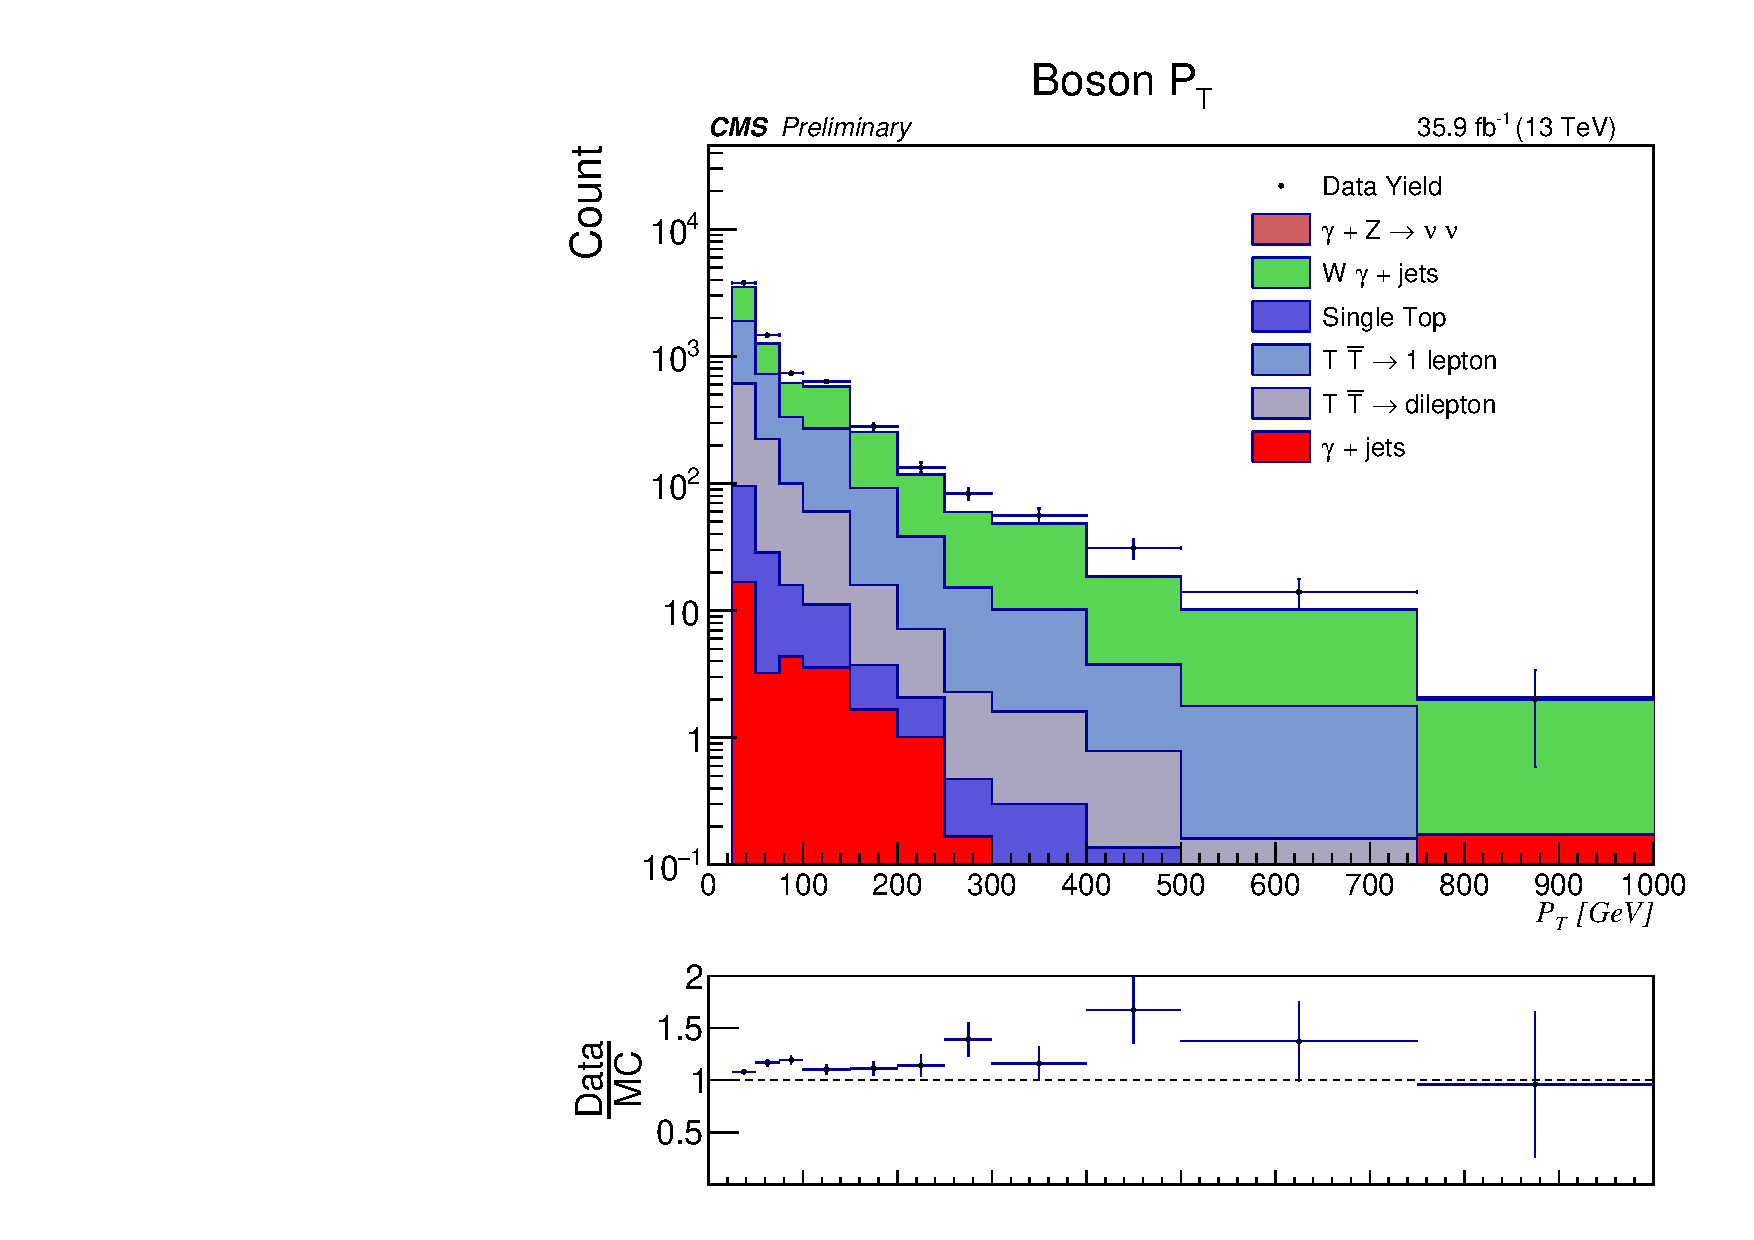
\includegraphics[width=.46\textwidth]{figures/datavsmc/mugamma/BosonPT_widebin.pdf}
        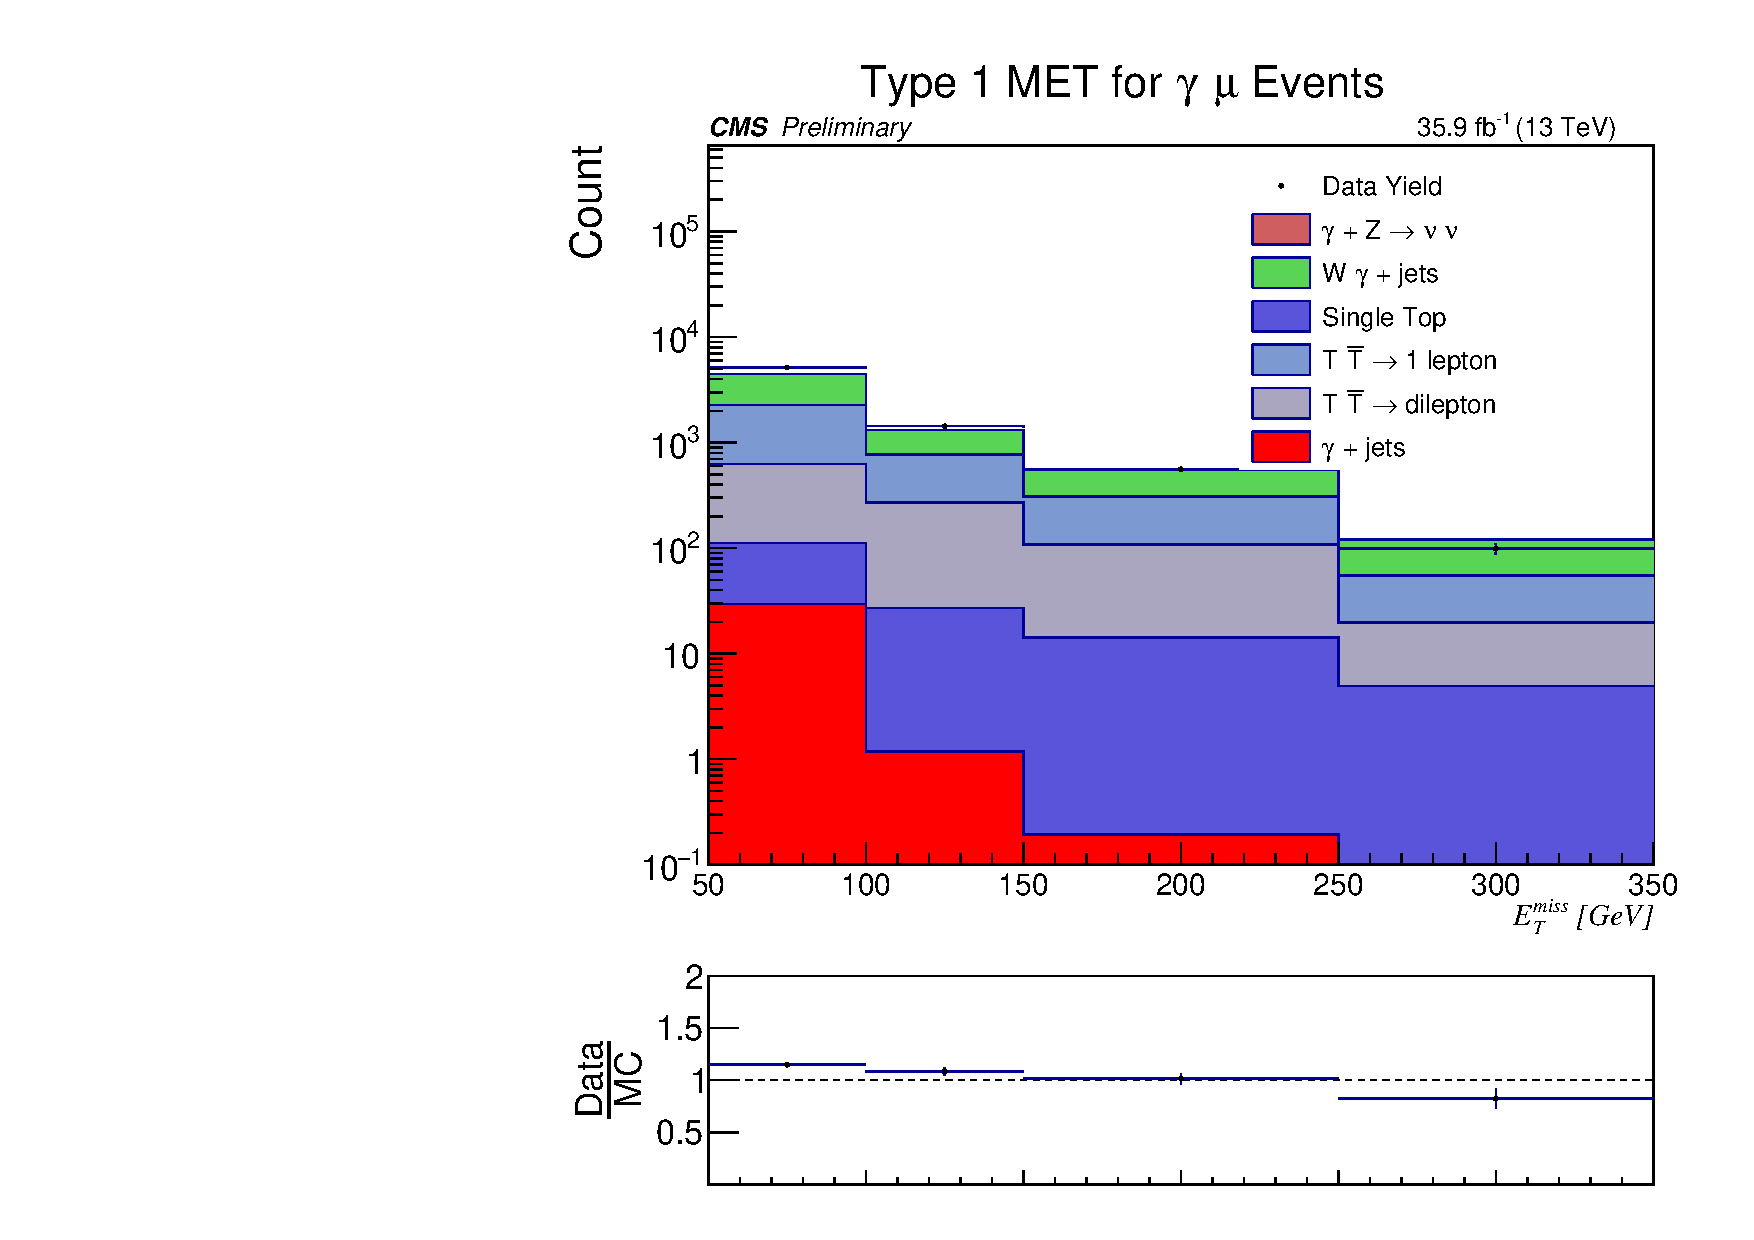
\includegraphics[width=.46\textwidth]{figures/datavsmc/mugamma/Type1MET_SRBin.pdf}
        \caption{The \pt (left) and \MET (right) profiles in simulation and data for the $\gamma \mu$ control sample, defined in sec \ref{sec:ewk_subtraction_closure_region}. The agreement between data and simulation is used to extract the expected fluctuation for the process of removing events with neutrinos from the $\gamma$+jets population. Given that the ratio is never deviates from unity by more than 30\% in the \MET profile, and mostly so in the \pt, we use 30\% as the systematic uncertainty for this process.}
        \label{fig:gamma_mu_closure}
      \end{figure}



    \subsubsection{Algorithm For The Prediction}

      Now that we have addressed the fundamental premise of this method and all the complications, we can give a full algorithm for the prediction:

      \begin{enumerate}
        \item Construct the population of single photon + jets events in the augmented search regions with dilepton quantities replaced by photon selection, full selection in sec \ref{sec:met_templates_control_region}.

        \item Simulate $\gamma+\nu$ events in MC, create a 'clean' population of only $\gamma+$jets events by subtracting the kinematic distributions of the $\gamma+\nu$ sample from any distribution of interest (in this case \pt).

        \item Take the `clean' photon sample and bin events by \pt in the intervals between (GeV): [25, 33, 40, 55, 85, 105, 135, 180, 250, $\infty$]. These are chosen to be just wide enough that there a high number of photon events in each bin, but fine enough to capture the \pt dependence of the jet configurations. 

        \item Create a `clean' Z+jets sample by taking the dilepton data that pass search region criteria, described in sec \ref{sec:search_regions}, and subtracting the other background predictions from any distribution of interest (in this case \pt). Note that the dilepton events are not binned in \MET at this point, all other cuts are applied.

        \item Normalize the area of the clean Z+jets \pt distribution and clean $\gamma+$jets to unity.

        \item Assign a weight to each photon event such that the bin has the same area as the corresponding Z+jets \pt bin.

        \item Construct the \MET profile of the cleaned $\gamma$+jets sample where each event is given the weight derived in the previous step.

        \item Find the ratio of the \MET 50-100 bin for the clean Z+jets sample vs. the clean $\gamma$+jets sample, apply this ratio across the entire cleaned $\gamma$+jets \MET profile

      \end{enumerate}

    \subsubsection{Systematics}

      The total uncertainty for this prediction is broken into 4 uncorrelated sources.

      \[
        \sigma^2_{\text{net}} = \sigma^2_{\text{Normalization}} +  \sigma^2_{\text{EWK Sub}} + \sigma^2_{\text{Statistical}} + \sigma^2_{\text{\pt Reweighting}}
      \]

      \begin{itemize}
        \bitem{Normalization} The uncertainty due to the cross section normalization of the $\gamma$+jets events to the Z+jets events in the \MET 50-100 bin. This is a percent uncertainty found on a bin-by-bin basis. The percentage is found by dividing the statistical uncertainty by the total count of events in the Z+jets \MET 50-100 bin. If the 50-100 \MET bin has a count of N events, a background prediction of $b$ in some higher \MET bin will get an uncertainty contribution of $ \sigma_{\text{Normalization}} = b \frac{\sigma(N)}{N}$ due to this source, where $\sigma(N)$ is the Poisson uncertainty for N events.

        \bitem{EWK Sub} The uncertainty due to the imperfect modeling of the $\gamma + \nu$ events when subtracting them from the $\gamma$+jets sample. A 30\% uncertainty is associated with the modeling of \pt and \MET as was shown in figure \ref{fig:gamma_mu_closure} and the section therein. This 30\% is applied to the total count of events subtracted from the \MET bin and scaled by the normalization from the \MET 50-100 bin. If $m_s$ events were subtracted from the $\gamma$+jets events in some \MET bin (after \pt reweighting), and $n$ is the normalization applied to the $\gamma$+jets sample to correct the cross section, the total uncertainty contribution to the \MET bin due to this source is $\sigma_{\text{EWK Sub}} = 0.3 \cdot n \cdot m_s$.

        \bitem{Statistical} The uncertainty due to the limited statistics of the $\gamma$+jets events. This is derived as a percent uncertainty on the \pt reweighted count of $\gamma$+jets events in a \MET bin. If a \MET bin has a background prediction of $b$ which was calculated from a $\gamma$+jets \MET bin with statistical uncertainty $\sigma_{\gamma}$, the total uncertainty contribution to the \MET bin due to this source is $\sigma_{\text{Statistical}} = \sigma_{\gamma} \cdot b$

        \bitem{\pt Reweighting} The uncertainty due to differences in the kinematics of jets in the photon and Z samples. The percent uncertainty for each \MET bin due to this source was summarized in table \ref{tab:template_systematics}. If a \MET bin has a background prediction of $b$ and the percent uncertainty due to the \pt reweighting is $p$, then the total uncertainty contribution to the \MET bin due to this source is $\sigma_{\text{\pt Reweighting}} = p \cdot b$.
      \end{itemize}

      A summary of all the Z+jets background predictions across all search bins as well as their systematics is shown below in table \ref{tab:template_systematics_summary}.

      \begin{table}[!h]
        \scriptsize
        \centering
        \caption{\label{tab:template_systematics_summary} A summary of all prediction counts and uncertainties for the Z+jets predictions. The number ``ratio" is the particular uncertainty associated for the process divided by the total uncertainty for the prediction in the \MET bin.
          }
        \begin{center}
          \begin{tabular} {l |l | l | l | l | l | l}
            SR & MET Bin & Prediction & Closure (ratio) & Normalization (ratio) & Statistical (ratio) & EWK Sub (ratio) \\ \hline
            SRA & 100-150 & 13.61 $\pm$ 3.14 & 2.72 (0.87) & 1.00 (0.32) & 1.14 (0.36) & 0.34 (0.11) \\
            & 150-250 & 2.45 $\pm$ 0.87 & 0.64 (0.74) & 0.18 (0.21) & 0.36 (0.42) & 0.42 (0.49) \\
            & 250+ & 3.26 $\pm$ 2.36 & 0.85 (0.36) & 0.24 (0.10) & 2.16 (0.91) & 0.39 (0.16) \\ \hline


            SRAb & 100-150 & 8.21 $\pm$ 2.10 & 1.64 (0.78) & 0.89 (0.42) & 0.92 (0.44) & 0.27 (0.13) \\
            & 150-250 & 1.19 $\pm$ 0.54 & 0.31 (0.57) & 0.13 (0.24) & 0.24 (0.45) & 0.35 (0.65) \\
            & 250+ & 0.51 $\pm$ 0.27 & 0.13 (0.48) & 0.05 (0.20) & 0.15 (0.56) & 0.18 (0.64) \\ \hline


            SRB & 100-150 & 12.81 $\pm$ 2.35 & 1.54 (0.65) & 1.19 (0.51) & 1.30 (0.56) & 0.16 (0.07) \\
            & 150-250 & 0.89 $\pm$ 0.34 & 0.13 (0.39) & 0.08 (0.24) & 0.22 (0.66) & 0.20 (0.59) \\
            & 250+ & 0.38 $\pm$ 0.20 & 0.06 (0.29) & 0.04 (0.18) & 0.12 (0.63) & 0.14 (0.69) \\ \hline


            SRBb & 100-150 & 7.74 $\pm$ 3.11 & 0.93 (0.30) & 1.32 (0.42) & 2.65 (0.85) & 0.23 (0.07) \\
            & 150-250 & 4.04 $\pm$ 3.33 & 0.73 (0.22) & 0.69 (0.21) & 3.16 (0.95) & 0.25 (0.07) \\
            & 250+ & 0.10 $\pm$ 0.14 & 0.02 (0.13) & 0.02 (0.12) & 0.04 (0.28) & 0.14 (0.94) \\ \hline


            SRC & 100-150 & 1.24 $\pm$ 0.43 & 0.19 (0.43) & 0.27 (0.64) & 0.27 (0.63) & 0.04 (0.09) \\
            & 150+ & 0.13 $\pm$ 0.11 & 0.04 (0.36) & 0.03 (0.27) & 0.05 (0.51) & 0.08 (0.74) \\ \hline


            SRCb & 100-150 & 0.14 $\pm$ 0.47 & 0.03 (0.06) & 0.05 (0.10) & 0.04 (0.08) & 0.47 (0.99) \\
            & 150+ & 0.00 $\pm$ 0.33 & 0.00 (0.00) & 0.00 (0.00) & 0.00 (0.00) & 0.33 (1.00) \\ \hline


            VZ & 100-150 & 29.27 $\pm$ 4.42 & 3.22 (0.73) & 1.13 (0.26) & 2.15 (0.49) & 1.81 (0.41) \\
            & 150-250 & 2.87 $\pm$ 2.09 & 0.69 (0.33) & 0.11 (0.05) & 0.40 (0.19) & 1.93 (0.92) \\
            & 250-350 & 1.00 $\pm$ 0.73 & 0.24 (0.33) & 0.04 (0.05) & 0.24 (0.33) & 0.64 (0.88) \\
            & 350+ & 0.29 $\pm$ 0.30 & 0.07 (0.23) & 0.01 (0.04) & 0.08 (0.26) & 0.28 (0.94) \\ \hline


            HZ & 100-150 & 2.90 $\pm$ 2.39 & 2.32 (0.97) & 0.34 (0.14) & 0.41 (0.17) & 0.24 (0.10) \\
            & 150-250 & 0.26 $\pm$ 0.19 & 0.09 (0.47) & 0.03 (0.16) & 0.08 (0.44) & 0.14 (0.75) \\
            & 250+ & 0.09 $\pm$ 0.07 & 0.03 (0.45) & 0.01 (0.16) & 0.05 (0.77) & 0.03 (0.42) \\ \hline

          \end{tabular}
        \end{center}
      \end{table}

  \clearpage

  \subsection{Flavor Symmetric Background} \label{sec:flavor_symmetric_background}
    
    The flavor symmetric background accounts for all cases where even a single lepton in the final dilepton pair was produced through the decay of a W boson. The basic idea is that the W has almost exactly the same decay rate to electrons and muons, therefore any event where a lepton was produced in a W decay should be mirrored by another event where the lepton was produced with the other flavor. In other words, if a physics process where a dilepton pair is produced and \emph{at least} one lepton came from a W boson occurs at some frequency $f$, a process where the dilepton pair has different flavor should occur with the same rate, $f$. The same argument holds for any flavor-symmetric process. For instance, ZZ production with two lost leptons, one from each Z, is also a flavor symmetric background because the chance to lose a muon is no different from the chance to lose an electron.\footnote{This is a rare process and those lost-lepton probabilities are not precisely identical, but the reader should understand that the existence of a W boson is not necessary to make a background process flavor symmetric. It is simply the most likely scenario as $t\bar{t}$ production is the only large cross section flavor-symmetric process in our search space.}

    Furthermore, given that the mass of the electron and the mass of the muon are many orders of magnitude less than the dilepton mass requirement of roughly 90 GeV, the typical energy scales and orientation of light leptons in flavor symmetric processes should be the same regardless of whether the leptons are paired with a same flavor or different flavor partner. This means that we can use the kinematical distributions in events with different flavor lepton pairs to predict the kinematical distributions for events with a same flavor lepton pair.

    In a totally idealized scenario, the flavor symmetric background prediction would be extremely simple. First, we would invert the selection for same flavor lepton pairs to require different flavor pairs in each \MET bin of our search regions. Then the count in each \MET for the different flavor pairs could be taken as the expected count for the search bin. However, as with any background prediction method, there are complications to our idealized scenario. 

    The first is that the \emph{reconstruction efficiency} for electrons and muons is not identical, meaning that there is a slight asymmetry between how likely the CMS detector and software suite are to find a muon vs. how likely they are to find an electron at some particular energy. This effect is caused by different detection methods used for electrons and muons. It manifests as different trigger efficiencies for electrons and muons at the same \pt, as briefly explained in sec \ref{sec:trigger_efficiencies}, as well the differences in the electron and muon ID requirements outlined in sections \ref{sec:electron_id_and_isolation} and \ref{sec:muon_id_and_isolation}. We correct for this effect with a factor called \rsfof, which is the subject of the next section.

    The second is that with few enough events, the symmetry between same-flavor and different-flavor pairs can be thrown off by statistical fluctuations.\footnote{Tossing a coin should yield as many heads as tails, however it is just as likely to get HH \emph{or} TT in tossing a coin twice as it is to get one of each. To chance to get an uneven percentage of heads or tails in a series of throws decreases with number of throws. The symmetry has more power with more statistics.} For this analysis, the expected number of flavor symmetric events in most search binds is less than 2. In order to ensure we have enough statistics for each prediction, the mass window for the acceptance of different flavor events is enlarged.

    With all corrections applied, the final number of events predicted in a \MET bin is 

    \begin{equation}
      N_{\text{SF}} = \kappa \cdot \rsfof \cdot N_{\text{DF}}, \label{eq:n_sf}
    \end{equation}

    where $\kappa$ is a corrective factor associated with the extrapolation from the enlarged mass window into the Z mass window, and \rsfof is a corrective factor associated with the asymmetry in electron and muon efficiencies.

    \subsubsection{The \rsfof Factor} \label{sec:rsfof}

      The factor \rsfof in eq. \ref{eq:n_sf} is a transfer factor which is meant to scale the number of different-flavor events in the flavor symmetric control regions, essentially the search regions with their same flavor requirement inverted, to the number of same-flavor events in associated search bin. This factor is derived through a direct measurement in the \rsfof control region, defined in sec. \ref{sec:rsfof_measurement_region} as $\MET \in [100,150]$, $\njets = 2$, and $\mll \notin [70,110]$. 

      The measurement of this factor is done in both data and $t\bar{t}$ MC, but the value MC is used only as a sanity check on the method. In order to set an uncertainty associated with this method, the \rsfof control region is binned further by various parameters that are used to construct the search regions. The variation in the measured value across these bins is used as the expected fluctuation of the method. These checks are shown in figure \ref{fig:rsfof_unc}.

      \begin{figure}[h!]
        \centering
        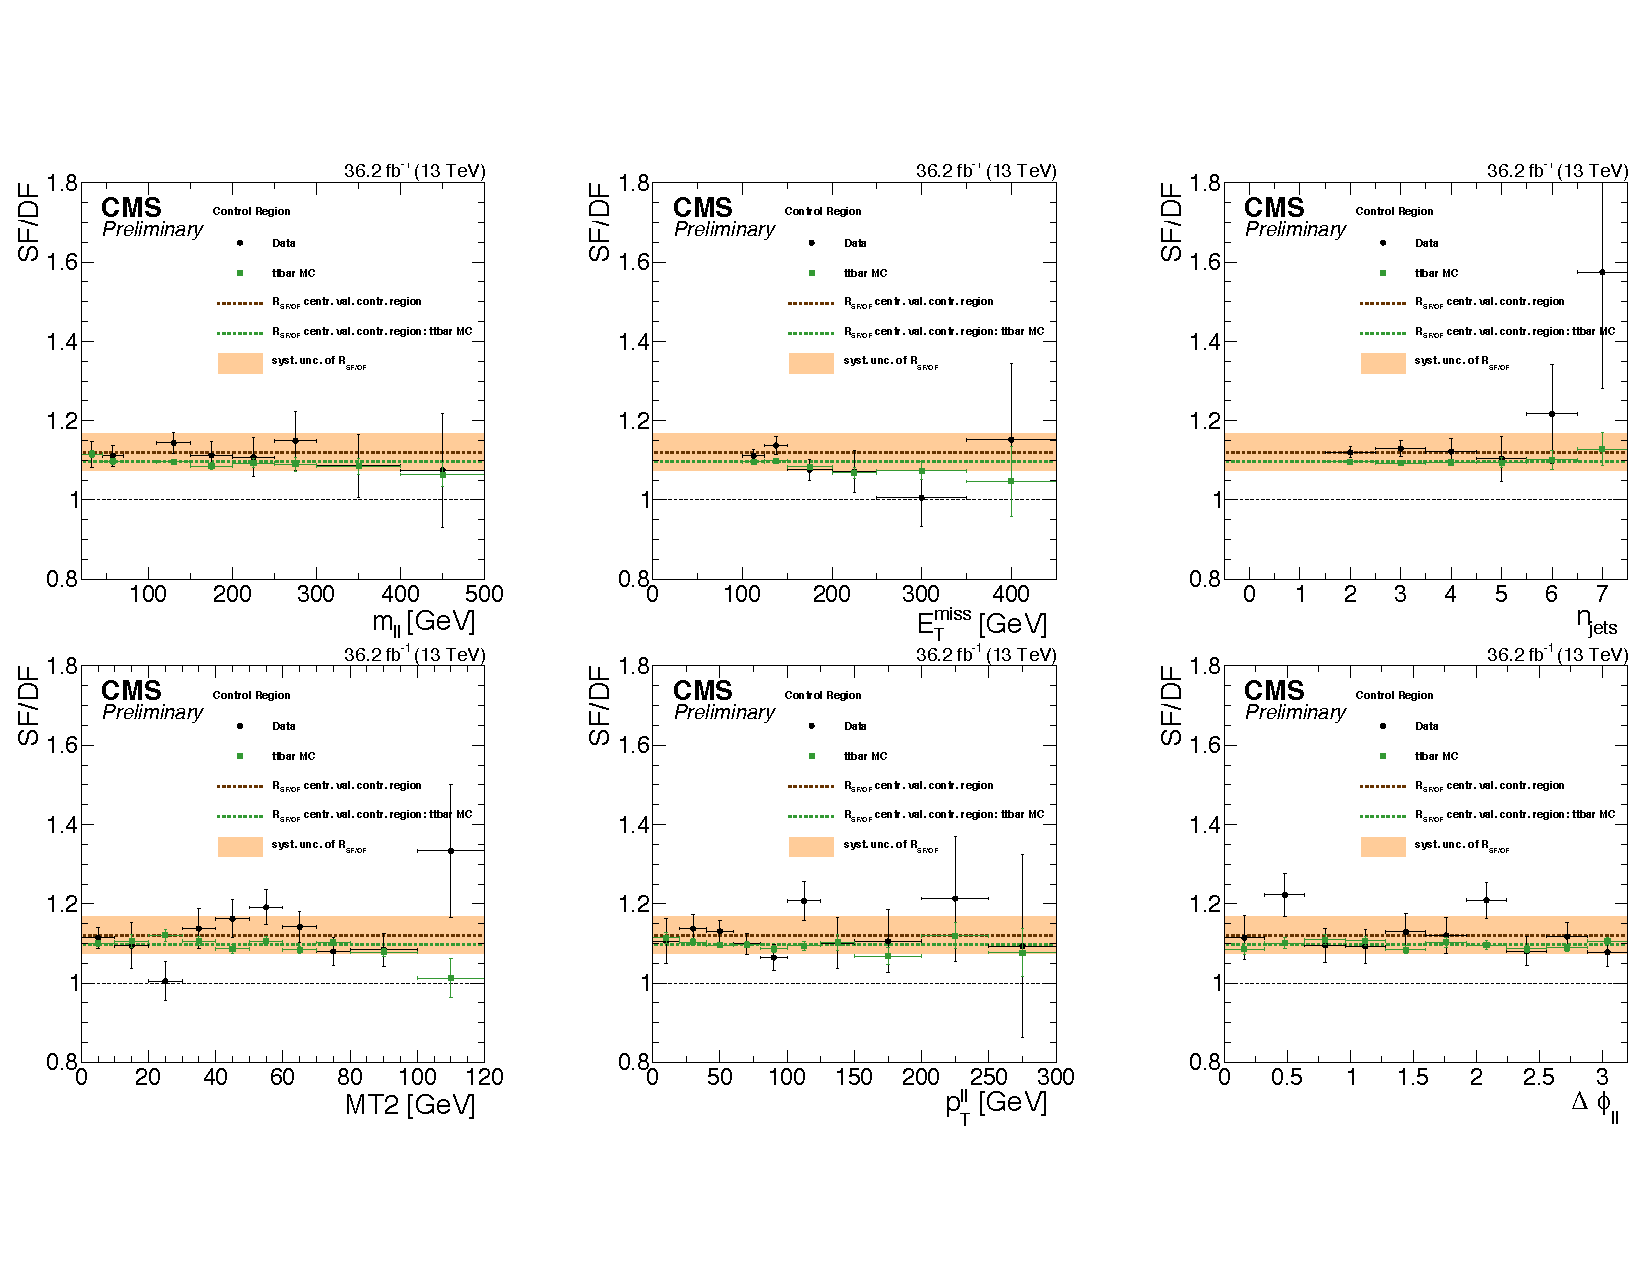
\includegraphics[width=\textwidth]{figures/RSFOF_Uncertainty.pdf}
        \caption{The measurement of \rsfof and its uncertainty. The \rsfof control region is further binned along the variables shown, and \rsfof is measured as they vary. The orange band shows the one-$\sigma$ expected fluctuation set by this method. As can be seen, the majority of data points fall within this orange band. \rsfof is relatively well behaved as a function of these kinematic and event-level variables.}
        \label{fig:rsfof_unc}
      \end{figure}

      The final value of \rsfof measured in data is $1.107 \pm 0.046$ (which is the value used in the final prediction), and the cross check in MC gives $1.090 \pm 0.005$.


    \subsubsection{Enlarging The Mass Window} \label{sec:kappa}

      In order to keep the statistical uncertainty reasonable, we enlarge the flavor symmetric control region's \mll window from $\pm 5$ GeV about the Z mass to $> 20$ GeV. Then we must apply a transfer factor, denoted by $\kappa$, which gives the ratio of number of events expected in this enlarged window, to the number of events expected in the Z mass window. 

      \[
        \kappa = \frac{\text{Num Different Flavor Events in Z Mass Window}}{\text{Num Different Flavor Events with \mll } > 20 \text{ GeV}}
      \]

      Furthermore, although \mll was chosen precisely because it is a relatively flat variable for $t\bar{t}$ events near the search regions, there are going to be some kinematic differences introduced by this asymmetry. In order to set an uncertainty associated with this method, we measure $\kappa$ in several control, search, and amalgamated search regions, defined in sec. \ref{sec:kappa_measurement_regions}. Simulated $t\bar{t}$ events are also used to measure $\kappa$ in these regions as a sanity check on the method to ensure there is little to no background contamination in the flavor symmetric control region. 

      The measured value of $\kappa$ is $0.065 \pm 0.02$ The $\kappa$ central value is then chosen to fit the various measured values. The one-$\sigma$ expected fluctuation is chosen such most values measured in data and all values measured in MC are within the band. Figure \ref{fig:kappa} summarized the measurements of $\kappa$ across all search and control regions in both data and MC. 

      \begin{figure}[h!]
        \centering
        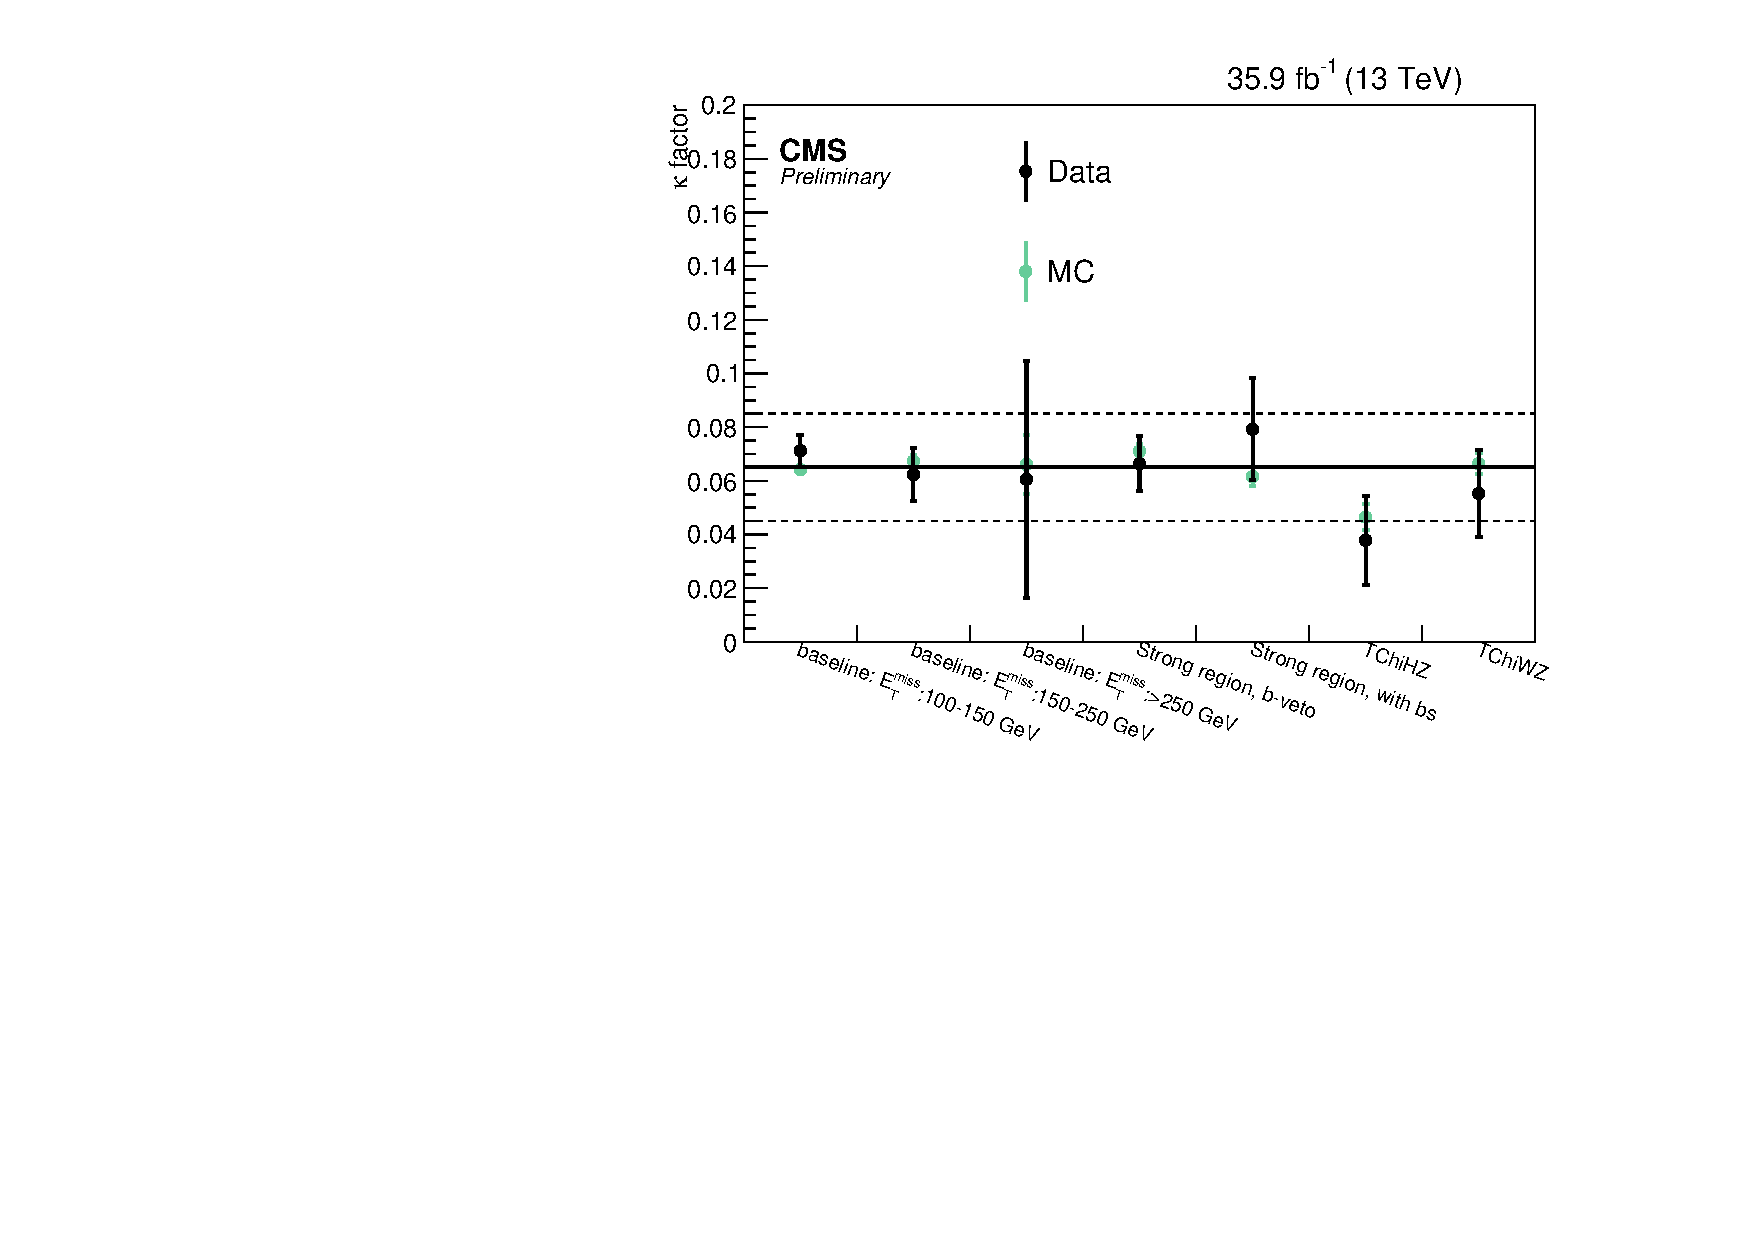
\includegraphics[width=\textwidth]{figures/datavsmc/data_summary_kfactors.pdf}
        \caption{The measurement of $\kappa$ across various search and control regions. The value measured in data and MC agree within uncertainty for all regions. The solid line is the central value chosen for $\kappa$ and the dashed lines represent the one-$\sigma$ expected fluctuations.}
        \label{fig:kappa}
      \end{figure}

      \clearpage

    \subsubsection{Systematics}

      The total uncertainty for this prediction is broken into 3 uncorrelated sources.

      \[
        \sigma^2_{\text{net}} = \sigma^2_{\text{\rsfof}} +  \sigma^2_{\kappa} + \sigma^2_{\text{Statistical}}
      \]

      The quantities $\sigma_{\text{\rsfof}}$ and $\sigma_{\kappa}$ are derived by taking the difference in the prediction when varying \rsfof and $\kappa$ between the two ends of their measured windows reported above. $\sigma_{\text{Statistical}}$ is the Poisson uncertainty on the number of events in the flavor symmetric control region associated the search bin scaled by the product of \rsfof and $\kappa$.

  \subsection{Z + $\nu$} \label{sec:z_+_neutrino}

    Table \ref{tab:znu_processes} summarizes the non-negligible background processes considered that can produce the Z+$\nu$ signature. The simulated events are only accepted when the dilepton pair can be matched back to a pair that came from a Z boson and there is a neutrino in the final state. This selection ensures there is no double counting background events that should be predicted by the flavor symmetric or Z+hadronic predictions.


    \begin{table}[!h]
      \centering
      \caption{\label{tab:znu_processes}
      A summary of the Z+$\nu$ background sources. These processes are simulated as described in sec \ref{sec:monte_carlo}. Only events which have a prompt neutrino and where the pair of selected leptons can be matched to a Z boson are considered to ensure orthogonality with the Z+jets and flavor symmetric background predictions.
      }
      \begin{center}
        \begin{tabular} {l | l}
        \hline
        \hline
        Category & Processes \\
        \hline
        WZ     & WZ$\to 3\ell + \nu$           \\
        ZZ     & 2$\ell + 2\nu$                \\
        TTZ    & Z$\to 2\ell$ and Z$\to 2\nu$  \\
        VVV    & ZZZ (inclusive decays)        \\
               & WZZ (inclusive decays)        \\
               & WWZ (inclusive decays)        \\
        \hline
        \hline
        \end{tabular}
      \end{center}
    \end{table}


    \subsubsection{Normalization Factors}
      Monte Carlo cross section are notoriously unreliable for low cross-section physics, especially in extreme regions of phase space used for new physics searches. In order to check the cross sections in the simulated events, the ZZ, WZ, and TTZ simulation are compared against data in specific control regions constructed to be sensitive to these processes. The full definitions of these control regions are given in sec \ref{sec:znu_control_regions}. Figure \ref{fig:rare_xsec_check} summarizes the results of these comparisons. 

      \begin{figure}[!h]
        \begin{center}
          \begin{tabular}{ccc}
            \begin{overpic}[width=0.3\textwidth]{figures/datavsmc/rare_xsec/WZ.pdf}    \put(30,68){\parbox{.5in}{\color{black} \small WZ Control Region}}     \end{overpic} &
            \begin{overpic}[width=0.3\textwidth]{figures/datavsmc/rare_xsec/ZZ.pdf}   \put(18,68){\parbox{.5in}{\color{black} \small ZZ \\ Control Region}}    \end{overpic} &
            \begin{overpic}[width=0.3\textwidth]{figures/datavsmc/rare_xsec/TTZ.pdf}    \put(18,68){\parbox{.5in}{\color{black} \small TTZ Control Region}}     \end{overpic} \\
          \end{tabular}
          \caption{ \normalsize Data and MC are compared in WZ, ZZ, and TTZ control regions in order to check whether the cross section in MC is compatible with what we see in data. The simulation is normalized such that the number of events in the control region in data and MC agree. \todo{Leonora made these, do I need to redo? Please god no...} \label{fig:rare_xsec_check}
          }
        \end{center}
      \end{figure}

      Due to the low cross section, difficulty of isolation, and low impact on the results, a rigorous analysis on the performance of simulation for these processes is not undertaken. Rather, a large conservative uncertainty is chosen based on the historical performance of simulating these models. \todo{How can I write this without saying we guess based on some heuristic crap.} A summary of derived normalization factors and the associated uncertainty in MC modeling is given in table \ref{tab:znu_norm_factors}.

      \begin{table}[!h]
      \centering
      \caption{\label{tab:znu_norm_factors}
      A summary of the Z+$\nu$ background sources' normalization factors and uncertainties. For the WZ, ZZ, and TTZ processes, normalization factors were found to correct the MC cross section, the VVV processes have low enough cross section that this is neglected. Due to the difficulty of isolating these processes and their low impact on search results, flat uncertainties are taken based on our level of confidence in MC performance.
      }
      \begin{center}
        \begin{tabular} {l | l | l}
        \hline
        \hline
        Sample & Normalization Factor & Percent Uncertainty \\
        \hline
        WZ     & 1.06                 & 30\%                \\
        ZZ     & 1.71                 & 50\%                \\
        TTZ    & 1.36                 & 30\%                \\
        VVV    & 1                    & 50\%                \\
        \hline
        \hline
        \end{tabular}
      \end{center}
    \end{table}

  \subsubsection{Systematics}

      The total uncertainty for this prediction is broken into 2 uncorrelated sources.

      \[
        \sigma^2_{\text{net}} = \sigma^2_{\text{MC Performance}} + \sigma^2_{\text{Statistical}}
      \]

      The statistical uncertainty is taken from the MC, the ``MC Performance" uncertainty is given in table \ref{tab:znu_norm_factors} above.

\section{Results} \label{sec:results}
  \subsection{Strong Search Regions} \label{sec:strong_search_regions}
    In this section, we show the search results for the strong signal regions. Figure \ref{fig:results_SR_str} shows the results visually, each search region is shown binned in \MET, the background predictions are broken down as described in \ref{sec:background_estimation_methods} and uncertainty bands are shown as a hashing that captures all sources described above. The number of events in data seen are shown as black dots in the figures. The same data is shown numerically in table \ref{tab:results_SR_str}.

    \begin{table}[!h]
      \scriptsize
      \centering
      \caption{\label{tab:results_SR_str} \todo{identical cap to AN}
      Results are shown for the strong signal regions.
      The uncertainties shown include both statistical and systematic errors. Note that the 50-100 \MET bin agrees perfectly by construction as it is used to normalize the DY prediction. See figure~\ref{fig:results_SR_str}~for the corresponding plots.
      }
      \begin{center}
        \begin{tabular} {l | l | l | l | l | l }
          SRA & \MET [GeV]  & 50-100 & 100-150 & 150-250 & 250+ \\ \hline 
          & Z+jets  & 208.5$\pm$16.1 & 13.6$\pm$3.1 & 2.5$\pm$0.9 & 3.3$\pm$2.4 \\
          & FS  & $0.4^{+0.3}_{-0.2}$  & $0.4^{+0.3}_{-0.2}$  & $0.2^{+0.2}_{-0.1}$  & $0.2^{+0.2}_{-0.1}$  \\
          & Z+$\nu$  & 1.1$\pm$0.4 & 0.8$\pm$0.3 & 1.4$\pm$0.4 & 2.4$\pm$0.8 \\ 
          & Sum  & $210.0^{+16.1}_{-16.1}$  & $14.8^{+3.2}_{-3.2}$  & $4.0^{+1.0}_{-1.0}$  & $5.9^{+2.5}_{-2.5}$ \\ 
          & Data  & 210 & 23 & 5 & 4 \\ \hline 


          SRAb & \MET [GeV]  & 50-100 & 100-150 & 150-250 & 250+ \\ \hline 
          & Z+jets  & 92.2$\pm$10.4 & 8.2$\pm$2.1 & 1.2$\pm$0.5 & 0.5$\pm$0.3 \\
          & FS  & $1.9^{+0.7}_{-0.7}$  & $2.3^{+0.8}_{-0.8}$  & $1.7^{+0.7}_{-0.6}$  & $0.1^{+0.2}_{-0.1}$  \\
          & Z+$\nu$  & 1.9$\pm$0.4 & 1.9$\pm$0.4 & 2.0$\pm$0.5 & 1.8$\pm$0.6 \\ 
          & Sum  & $96.0^{+10.4}_{-10.4}$  & $12.4^{+2.3}_{-2.3}$  & $4.9^{+1.0}_{-1.0}$  & $2.5^{+0.7}_{-0.7}$ \\ 
          & Data  & 96 & 14 & 7 & 1 \\ \hline 


          SRB & \MET [GeV]  & 50-100 & 100-150 & 150-250 & 250+ \\ \hline 
          & Z+jets  & 130.1$\pm$12.8 & 12.8$\pm$2.3 & 0.9$\pm$0.3 & 0.4$\pm$0.2 \\
          & FS  & $0.3^{+0.2}_{-0.2}$  & $0.4^{+0.3}_{-0.2}$  & $0.4^{+0.3}_{-0.2}$  & $0.1^{+0.2}_{-0.1}$  \\
          & Z+$\nu$  & 0.6$\pm$0.2 & 0.3$\pm$0.1 & 0.7$\pm$0.2 & 1.2$\pm$0.4 \\ 
          & Sum  & $131.0^{+12.8}_{-12.8}$  & $13.6^{+2.4}_{-2.4}$  & $2.0^{+0.5}_{-0.5}$  & $1.6^{+0.5}_{-0.4}$ \\ 
          & Data  & 131 & 10 & 4 & 0 \\ \hline 


          SRBb & \MET [GeV]  & 50-100 & 100-150 & 150-250 & 250+ \\ \hline 
          & Z+jets  & 37.9$\pm$6.7 & 7.7$\pm$3.1 & 4.0$\pm$3.3 & 0.1$\pm$0.1 \\
          & FS  & $0.7^{+0.4}_{-0.3}$  & $1.4^{+0.6}_{-0.5}$  & $1.1^{+0.5}_{-0.4}$  & $0.2^{+0.2}_{-0.1}$  \\
          & Z+$\nu$  & 1.3$\pm$0.4 & 2.0$\pm$0.5 & 2.3$\pm$0.6 & 1.0$\pm$0.3 \\ 
          & Sum  & $40.0^{+6.8}_{-6.8}$  & $11.1^{+3.2}_{-3.2}$  & $7.4^{+3.4}_{-3.4}$  & $1.3^{+0.4}_{-0.3}$ \\ 
          & Data  & 40 & 10 & 5 & 0 \\ \hline 


          SRC & \MET [GeV]  &  50-100 &  100-150 & \multicolumn{2}{l}{ 150+ } \\ \hline 
          & Z+jets  &  23.8$\pm$5.5 &  1.2$\pm$0.4 & \multicolumn{2}{l}{ 0.1$\pm$0.1 } \\ 
          & FS  &  $0.1^{+0.2}_{-0.1}$  &  $0.4^{+0.3}_{-0.2}$  & \multicolumn{2}{l}{ $0.1^{+0.2}_{-0.1}$  } \\ 
          & Z+$\nu$  &  0.2$\pm$0.1 &  0.1$\pm$0.1 & \multicolumn{2}{l}{ 0.5$\pm$0.2 } \\ 
          & Sum  &  $24.0^{+5.5}_{-5.5}$  &  $1.7^{+0.5}_{-0.5}$  & \multicolumn{2}{l}{ $0.7^{+0.3}_{-0.2}$ } \\ 
          & Data  &  24 &  4 & \multicolumn{2}{l}{ 0 } \\ \hline 


          SRCb & \MET [GeV]  &  50-100 &  100-150 & \multicolumn{2}{l}{ 150+ } \\ \hline 
          & Z+jets  &  9.9$\pm$3.7 &  0.1$\pm$0.5 & \multicolumn{2}{l}{ 0.0$\pm$0.3 } \\ 
          & FS  &  $0.1^{+0.2}_{-0.1}$  &  $0.0^{+0.1}_{-0.0}$  & \multicolumn{2}{l}{ $0.3^{+0.2}_{-0.2}$  } \\ 
          & Z+$\nu$  &  0.0$\pm$0.1 &  0.6$\pm$0.2 & \multicolumn{2}{l}{ 0.6$\pm$0.2 } \\ 
          & Sum  &  $10.0^{+3.7}_{-3.7}$  &  $0.8^{+0.5}_{-0.5}$  & \multicolumn{2}{l}{ $0.9^{+0.5}_{-0.4}$ } \\ 
          & Data  &  10 &  2 & \multicolumn{2}{l}{ 2 } \\ \hline 

        \end{tabular}
      \end{center}
    \end{table}

    \begin{figure}[!htb]
      \centering
      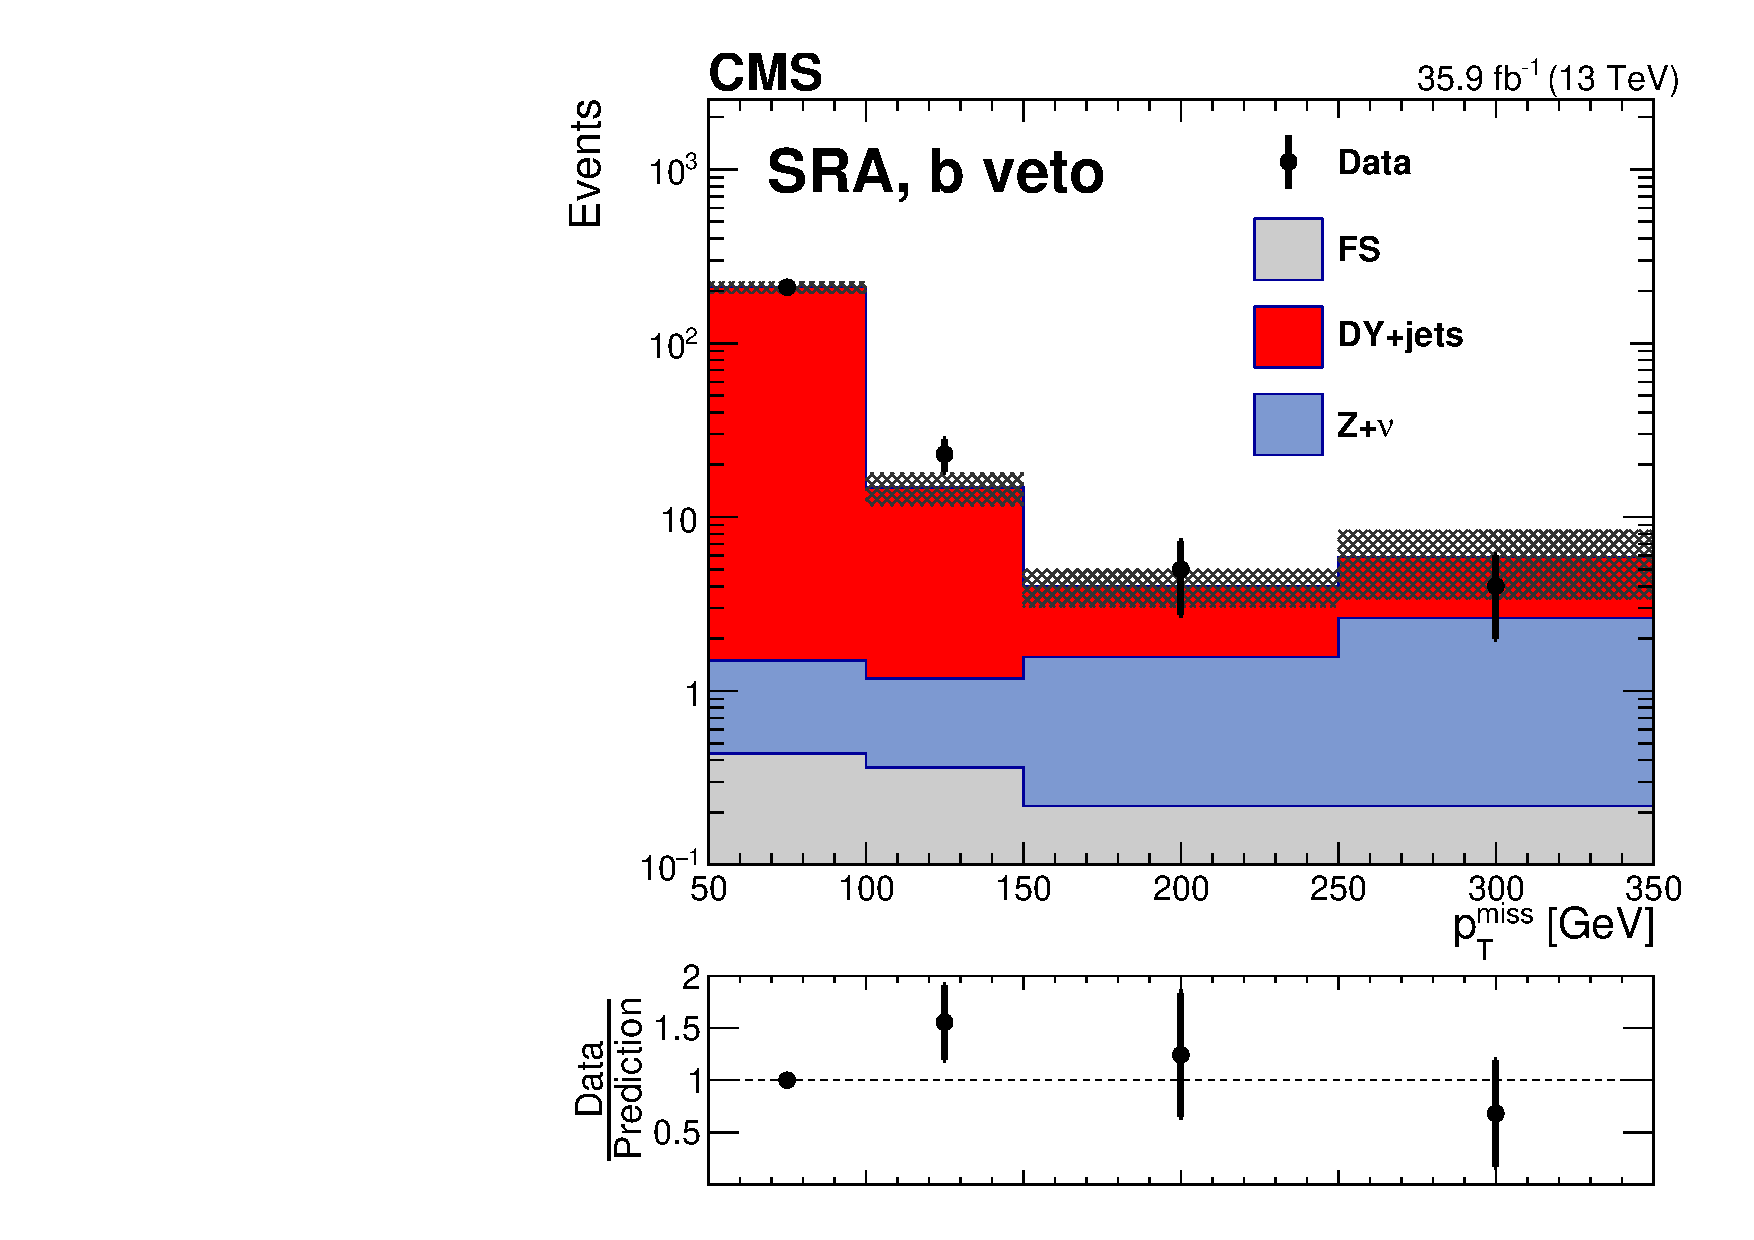
\includegraphics[width=0.35\linewidth]{figures/results/h_met_SR_2jbv.pdf}%
      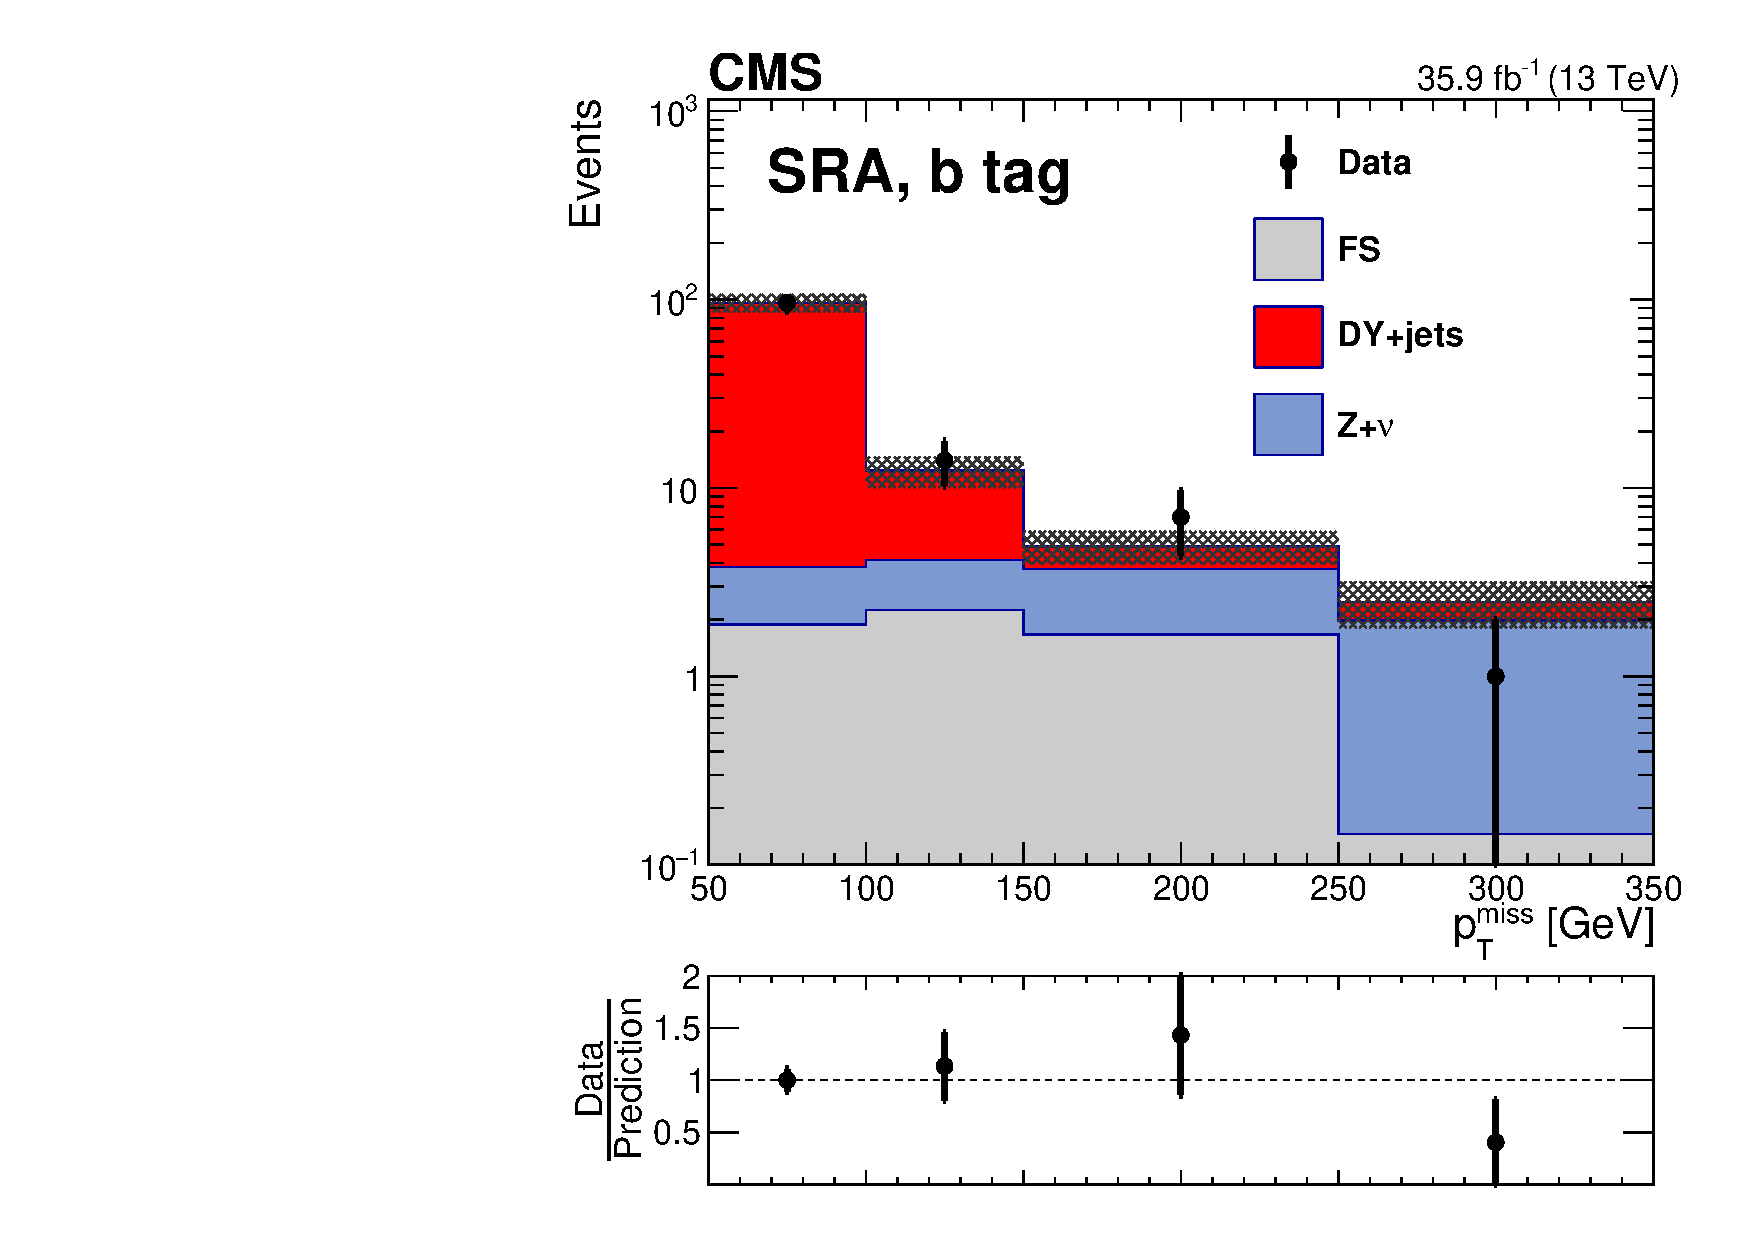
\includegraphics[width=0.35\linewidth]{figures/results/h_met_SR_2jbt.pdf}
      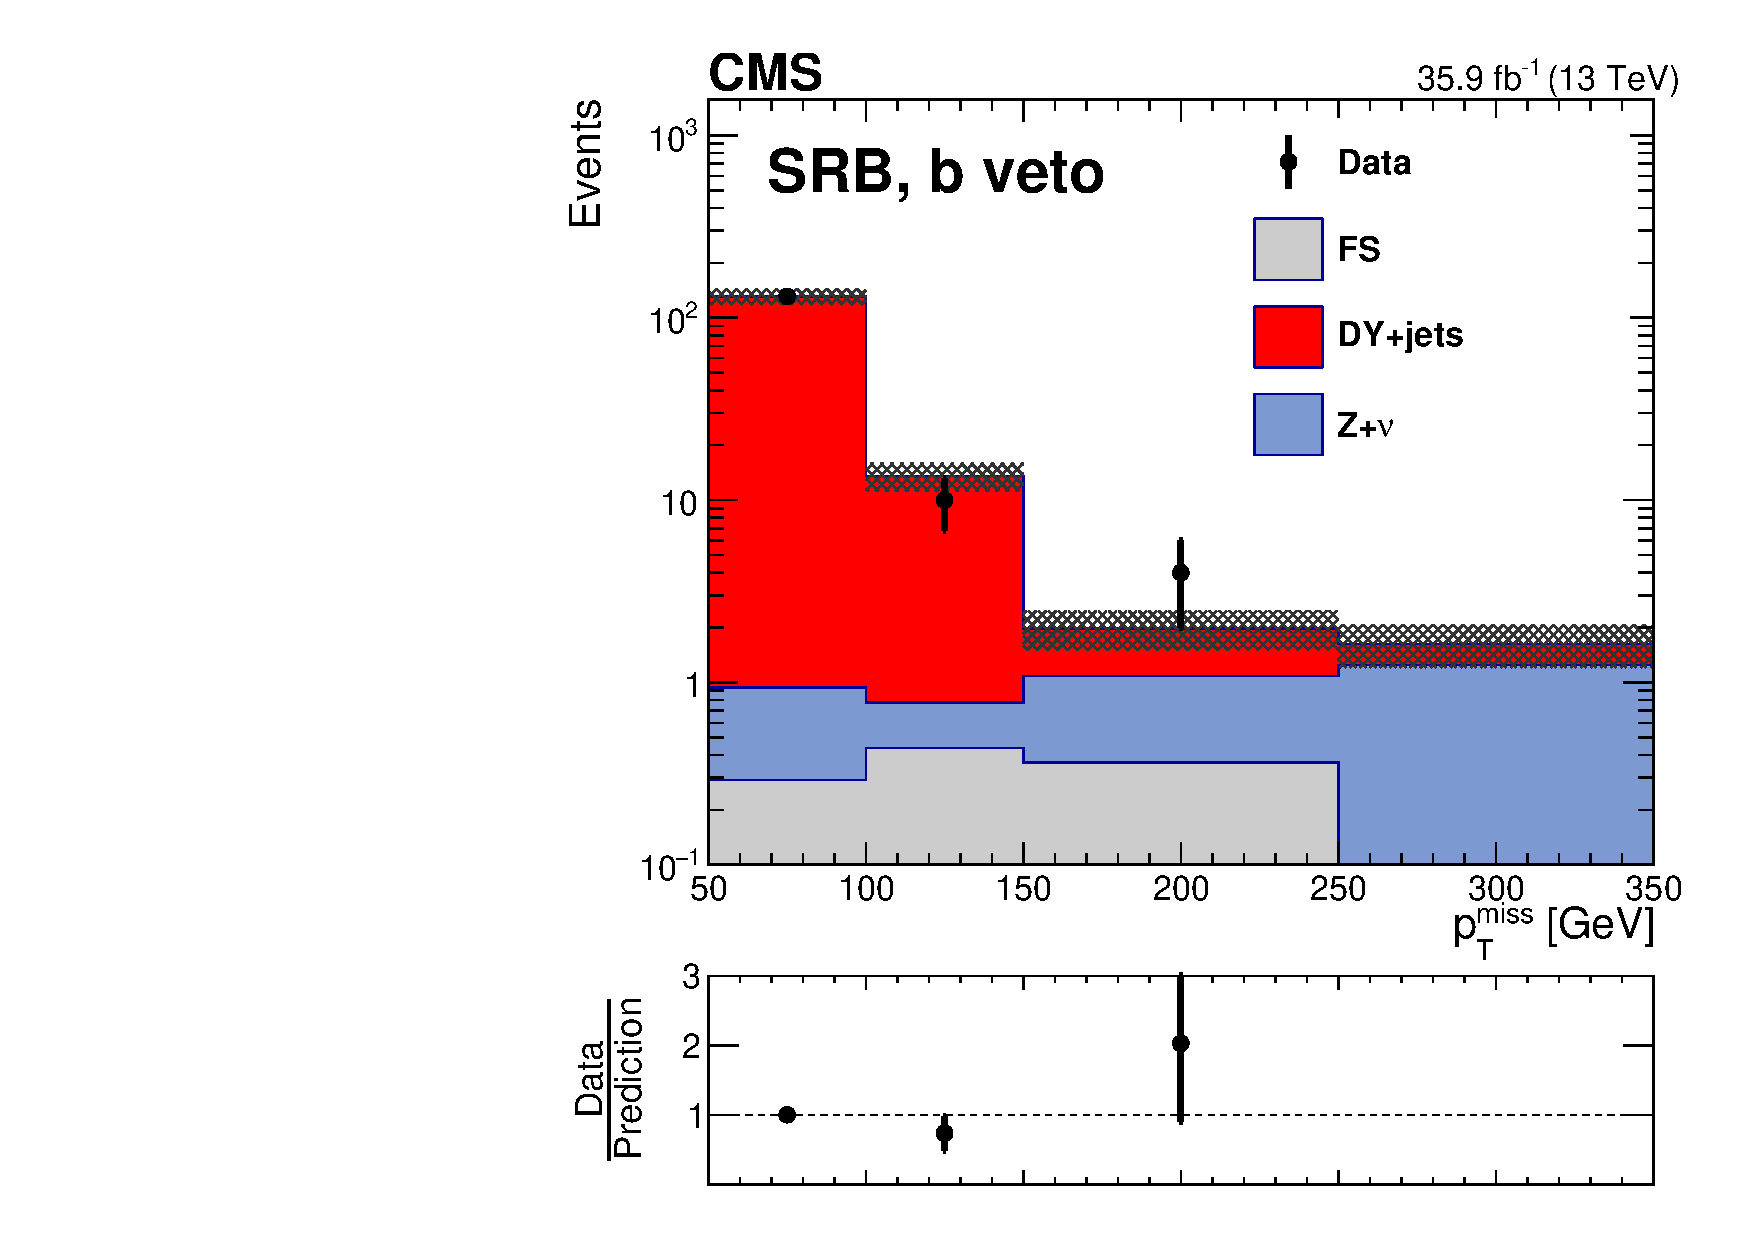
\includegraphics[width=0.35\linewidth]{figures/results/h_met_SR_4jbv.pdf}%
      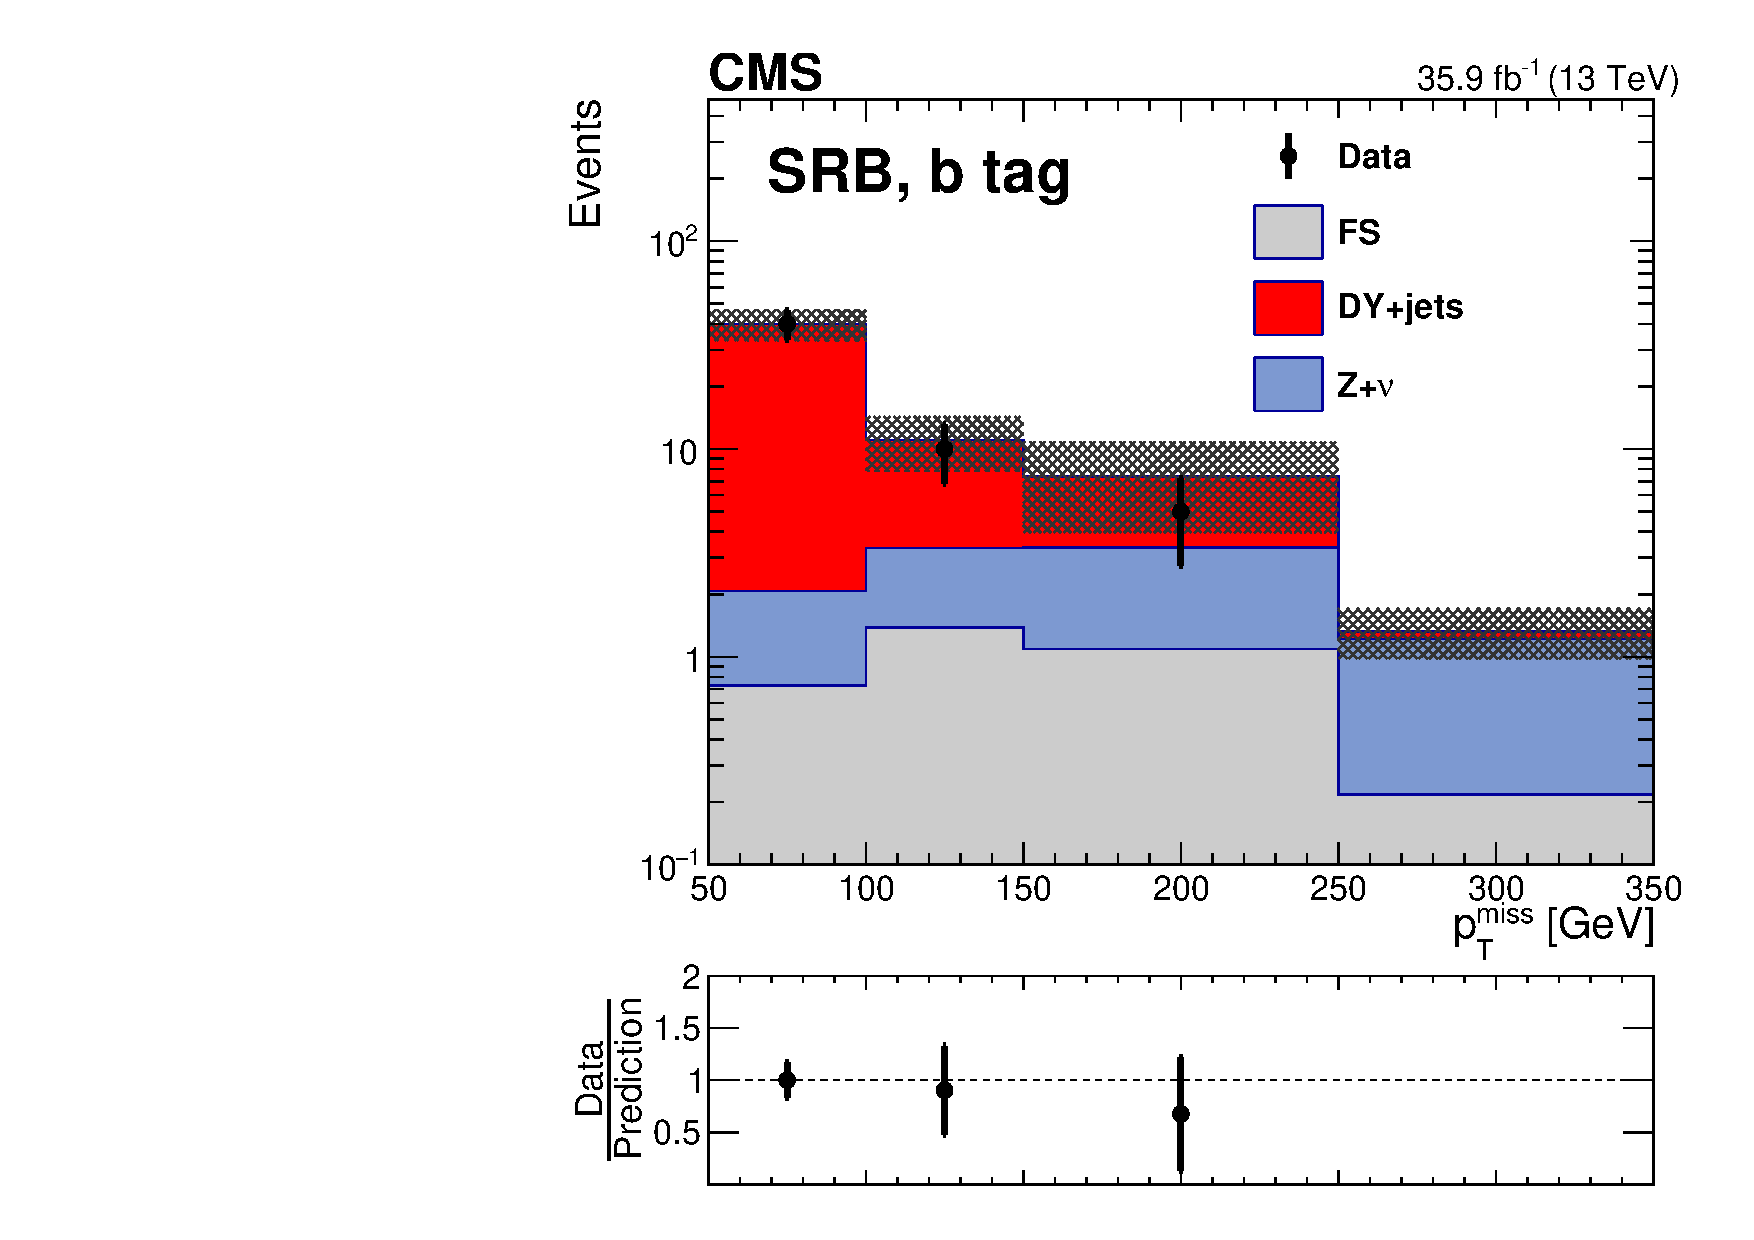
\includegraphics[width=0.35\linewidth]{figures/results/h_met_SR_4jbt.pdf}
      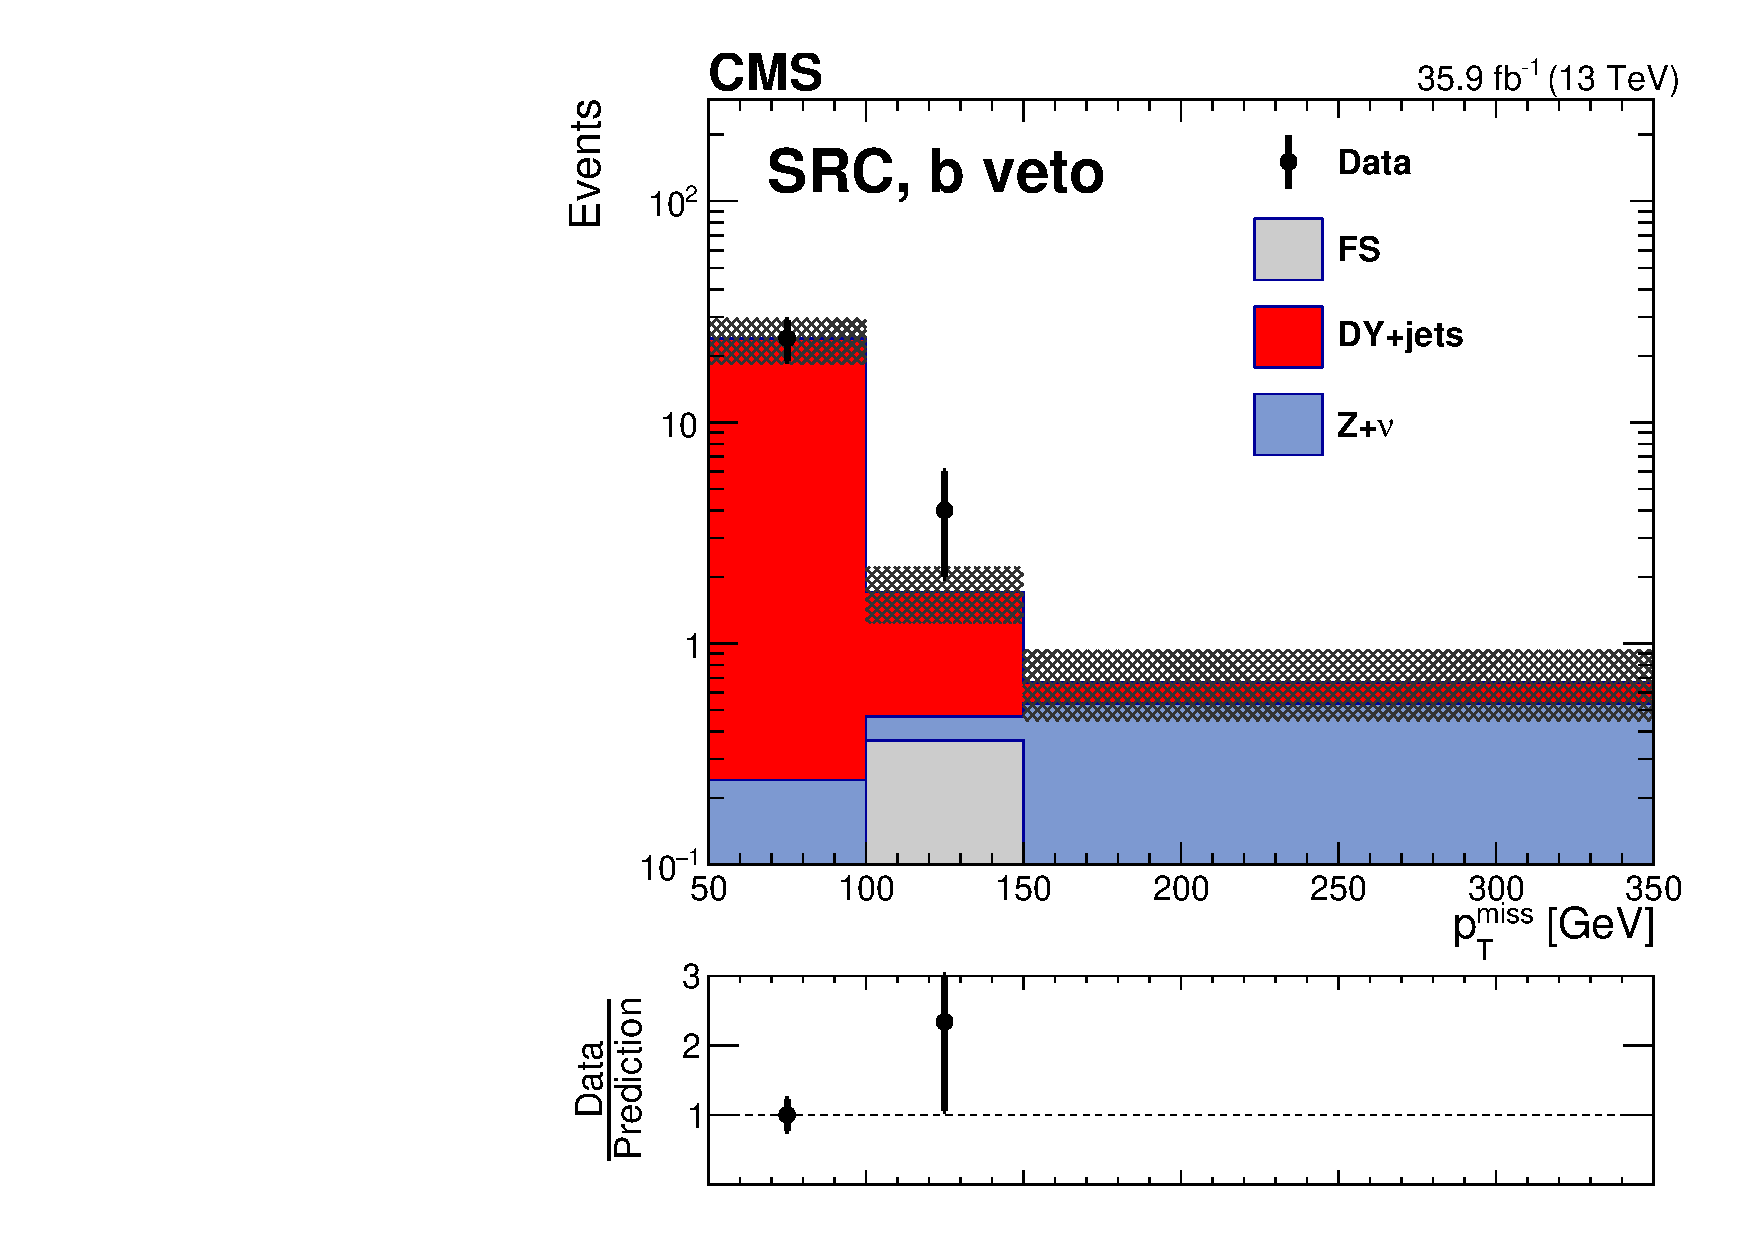
\includegraphics[width=0.35\linewidth]{figures/results/h_met_SR_6jbv.pdf}%
      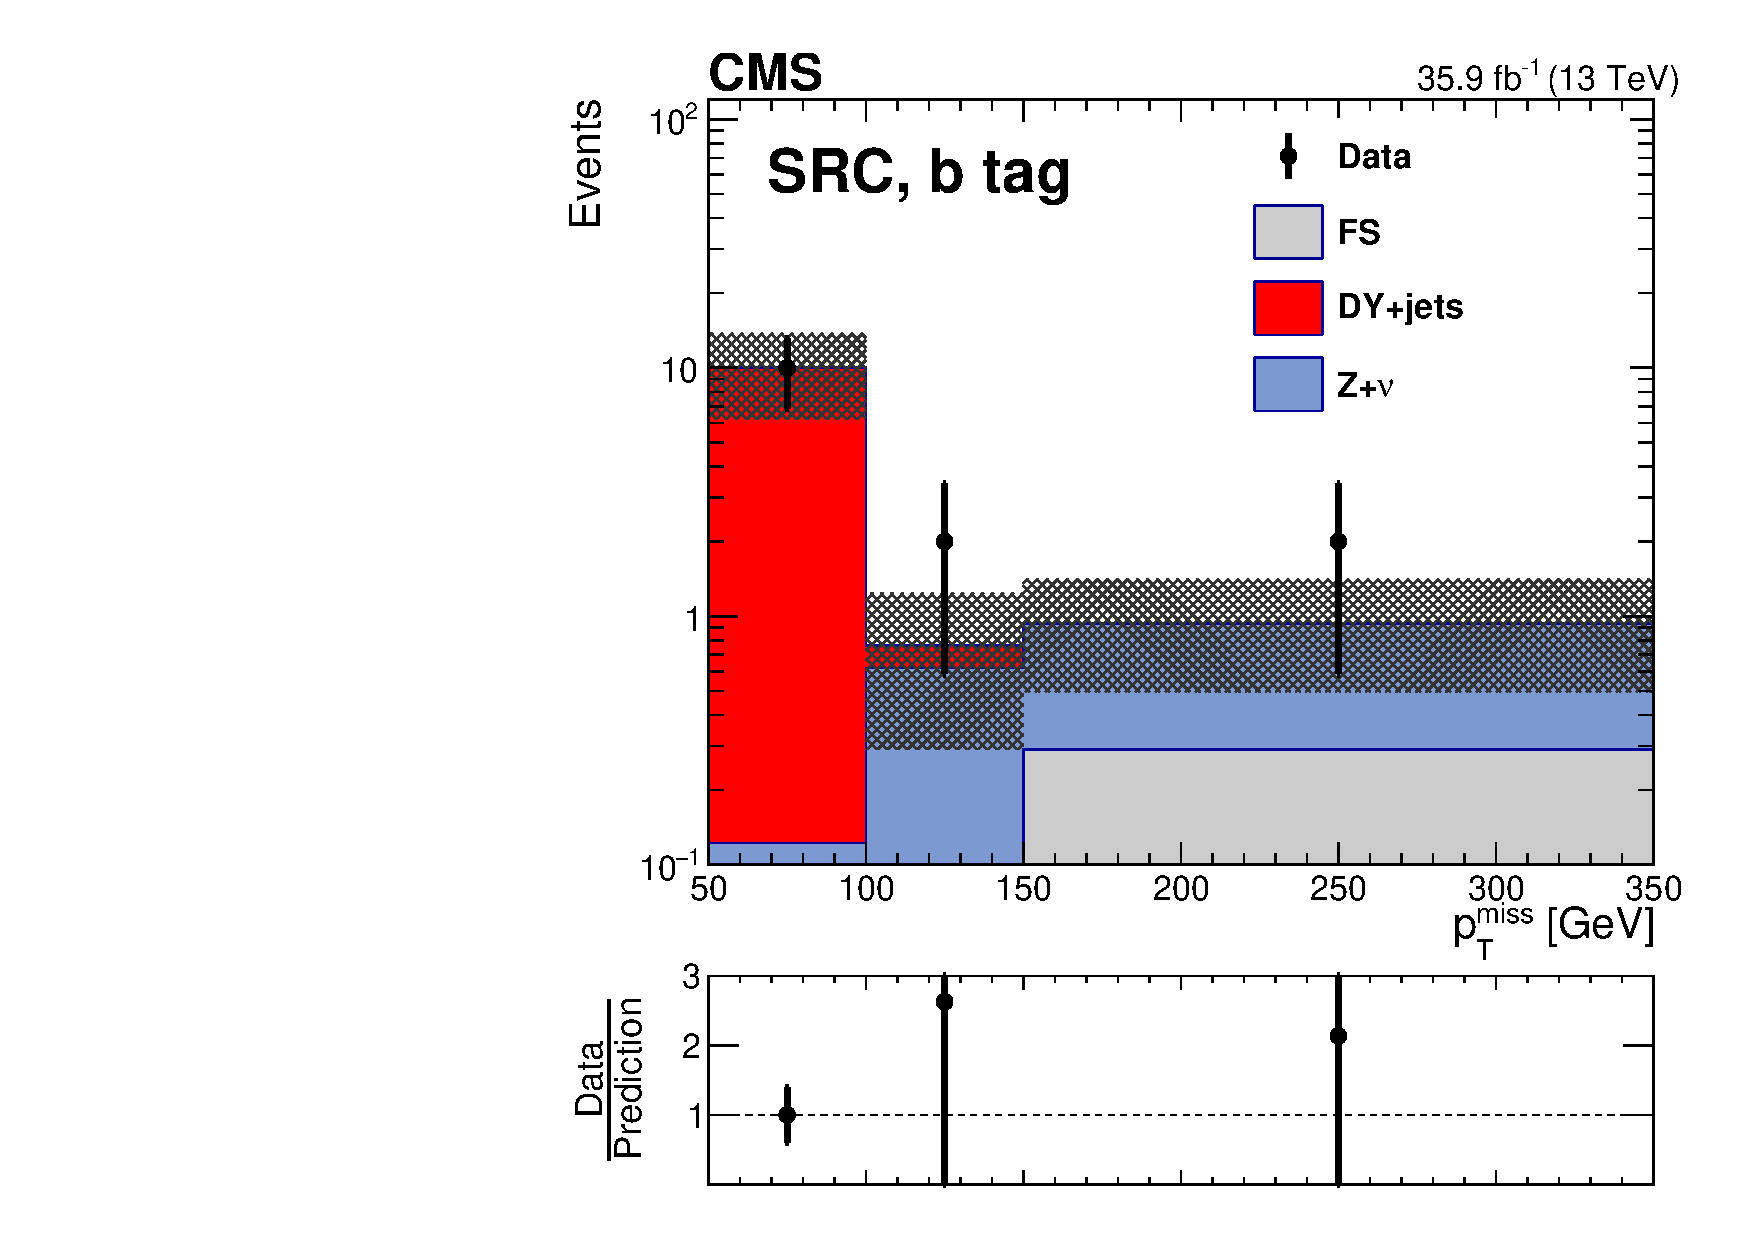
\includegraphics[width=0.35\linewidth]{figures/results/h_met_SR_6jbt.pdf}
      \caption{\label{fig:results_SR_str} \todo{identical cap to AN}
      The \MET distribution is shown for data vs. the data-driven predictions in the strong signal regions with $\nb = 0$ (left) and $\nb \geq 1$ (right).
      The top row shows events in SRA which are required to have 2-3 jets and \HT\ $>$ 500 (200)~GeV for events with exactly 0 bjets (at least one bjet),
      the second row shows events in SRB which are required to have 4-5 jets and \HT\ $>$ 500 (200)~GeV for events with exactly 0 bjets (at least one bjet),
      and the bottom row shows events in SRC which are required to have $\geq$~6 jets.
      Note that the 50-100 \MET bin agrees perfectly by construction as it is used to normalize the DY prediction. The yields for these plots are shown in table~\ref{tab:results_SR_str}.
      }
    \end{figure}

  \clearpage

  \subsection{Electroweak Search Regions}

    The following shows the results for the electroweak search regions. 

    \begin{figure}[!h]
      \centering
      \begin{tabular}{cc}
        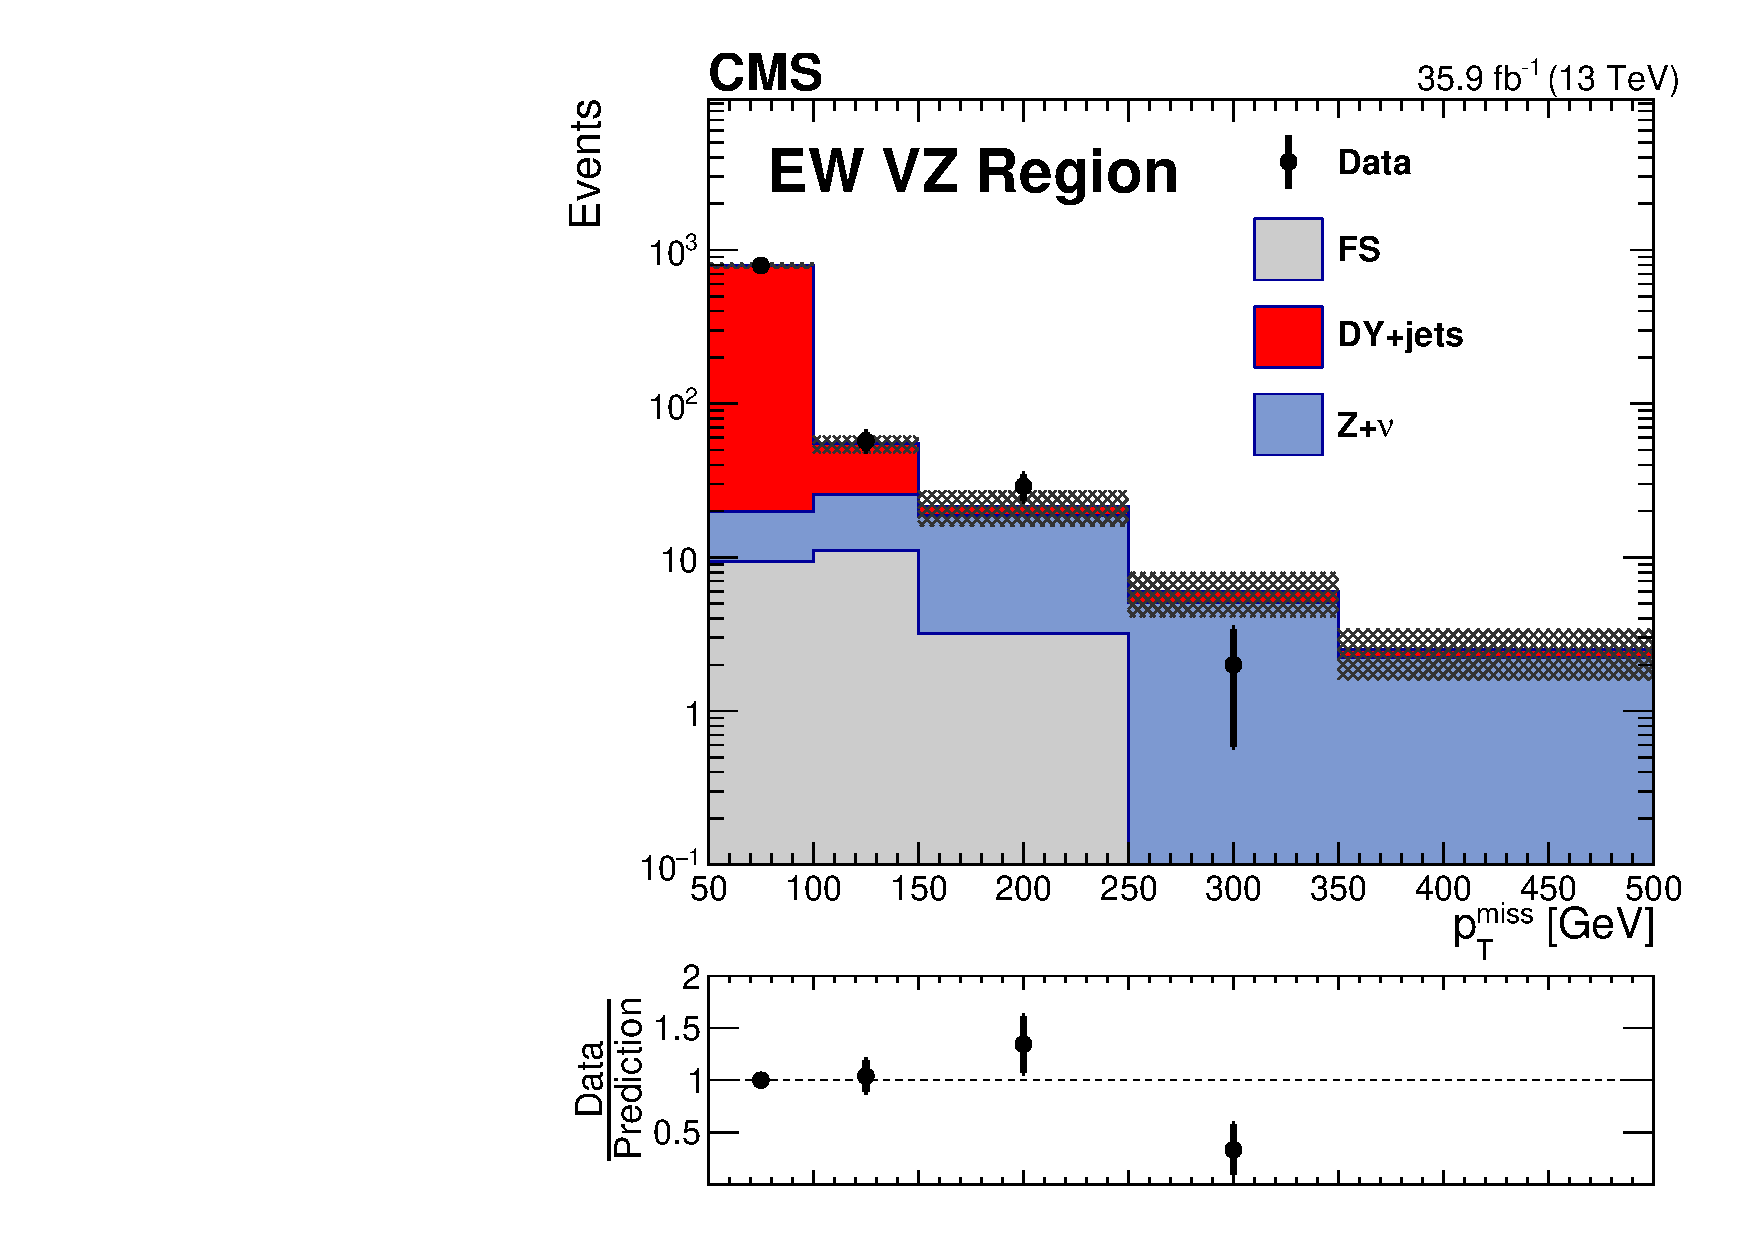
\includegraphics[width=0.4\linewidth]{figures/results/h_met_SR_tcwz.pdf} &
        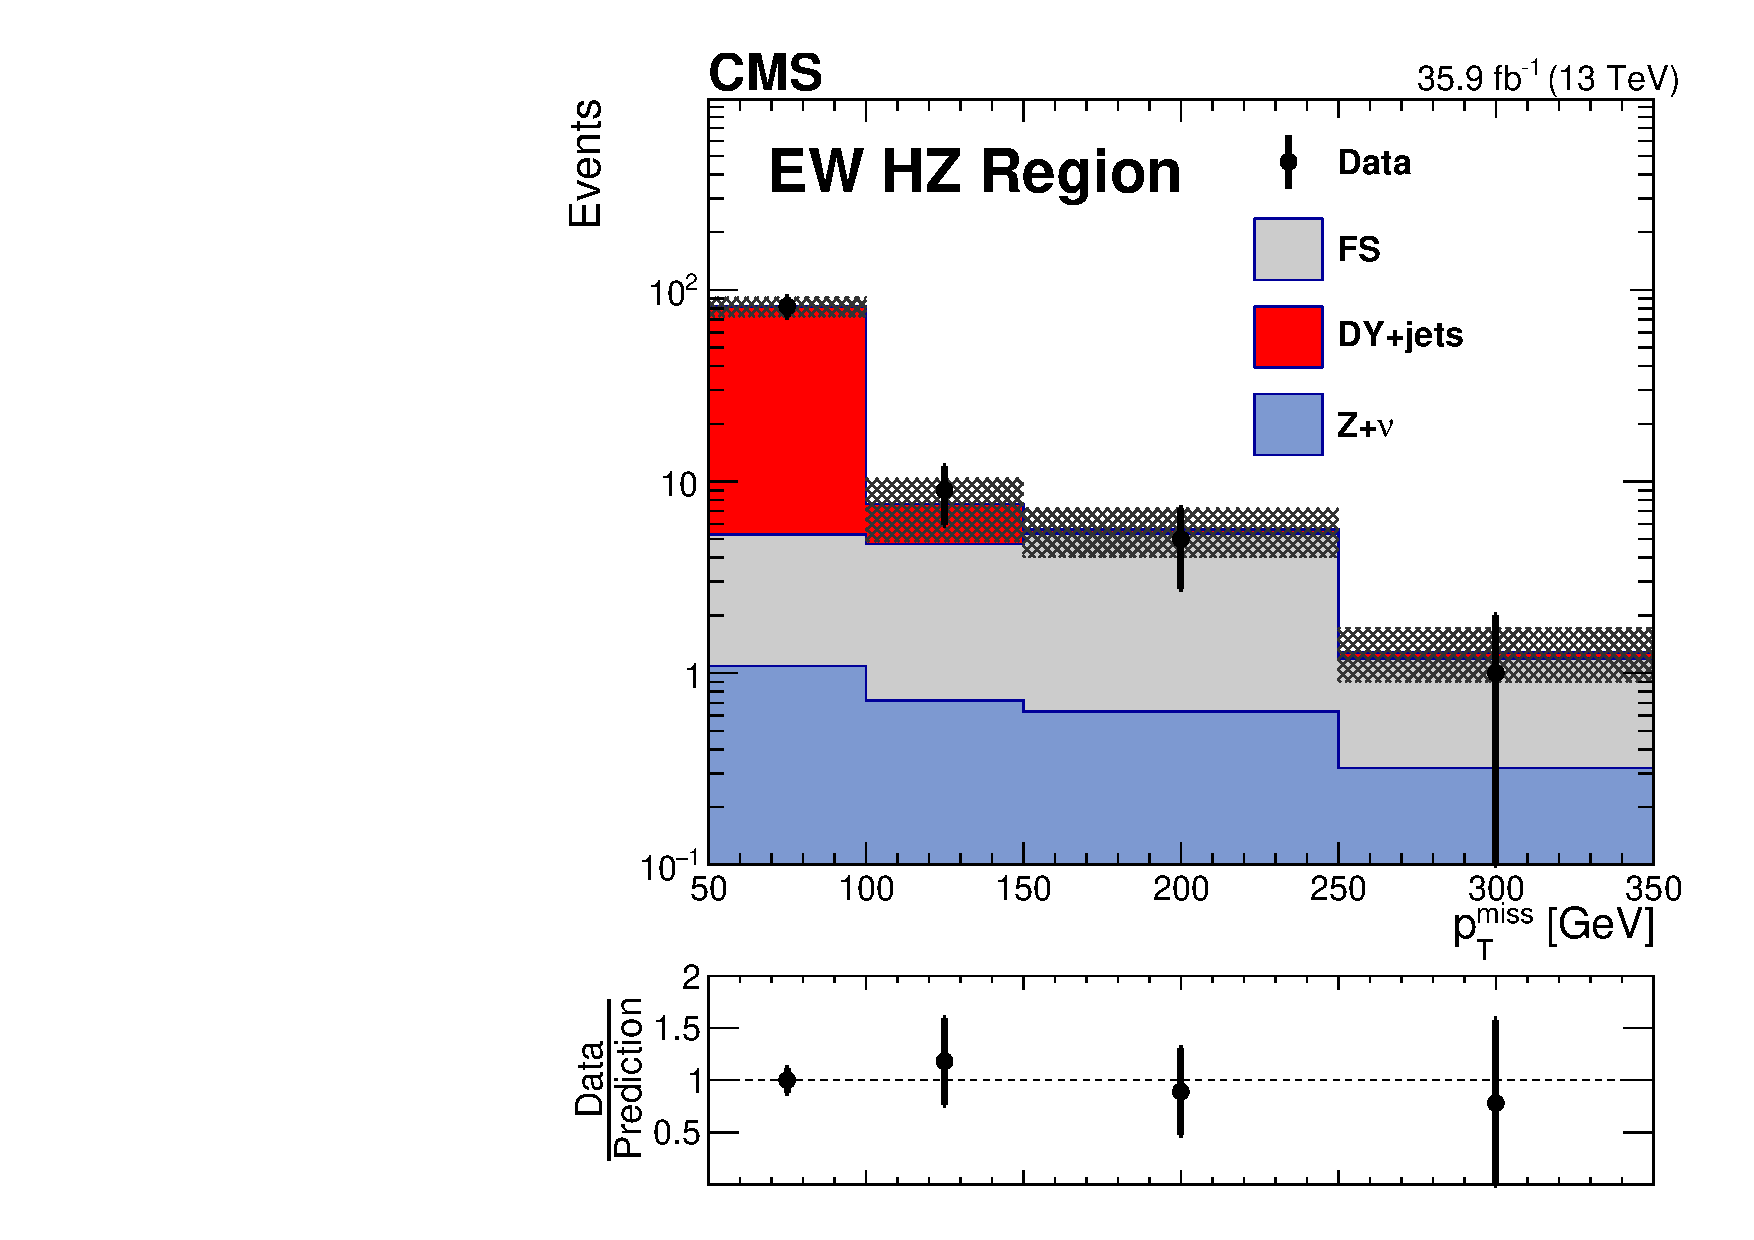
\includegraphics[width=0.4\linewidth]{figures/results/h_met_SR_tchz.pdf} \\
      \end{tabular}
      \caption{\todo{identical cap to AN}
        The \MET\ distribution is shown for data vs. the data-driven predictions in the TChiWZ/ZZ (left), and TChiHZ (right) signal regions. Note that the 50-100 MET bin agrees perfectly by construction as it is used to normalize the DY prediction. See table~\ref{tab:results_SR_ewk}~for yields.
        \label{fig:results_SR_ewk}
      }
    \end{figure}

    \begin{table}[!htb]
      \scriptsize
      \centering
      \caption{\label{tab:results_SR_ewk} \todo{identical cap to AN}
      Results are shown for the electroweak signal regions.
      The uncertainties shown include both statistical and systematic errors. Note that the 50-100 \MET bin agrees perfectly by construction as it is used to normalize the DY prediction. See figure~\ref{fig:results_SR_ewk}~for the corresponding plots.
      }
      \begin{center}
        \begin{tabular} {l | l | l | l | l | l | l }
          VZ & \MET [GeV]  & 50-100 & 100-150 & 150-250 & 250-350 & 350+ \\ \hline 
          & Z+jets  & 773.2$\pm$31.9 & 29.3$\pm$4.4 & 2.9$\pm$2.1 & 1.0$\pm$0.7 & 0.3$\pm$0.3 \\
          & FS  & $9.4^{+3.0}_{-3.0}$  & $11.1^{+3.6}_{-3.6}$  & $3.2^{+1.1}_{-1.1}$  & $0.1^{+0.2}_{-0.1}$  & $0.1^{+0.2}_{-0.1}$  \\
          & Z+$\nu$  & 10.4$\pm$2.6 & 14.5$\pm$4.0 & 15.5$\pm$5.1 & 5.0$\pm$1.8 & 2.2$\pm$0.9 \\ 
          & Sum  & $793.0^{+32.2}_{-32.2}$  & $54.9^{+7.0}_{-7.0}$  & $21.6^{+5.6}_{-5.6}$  & $6.0^{+1.9}_{-1.9}$  & $2.5^{+0.9}_{-0.9}$ \\ 
          & Data  & 793 & 57 & 29 & 2 & 0 \\ \hline 


          HZ & \MET [GeV]  &  50-100 &  100-150 &  150-250 & \multicolumn{2}{l}{ 250+ } \\ \hline 
          & Z+jets  &  76.7$\pm$9.4 &  2.9$\pm$2.4 &  0.3$\pm$0.2 & \multicolumn{2}{l}{ 0.1$\pm$0.1 } \\ 
          & FS  &  $4.2^{+1.4}_{-1.4}$  &  $4.0^{+1.4}_{-1.4}$  &  $4.7^{+1.6}_{-1.6}$  & \multicolumn{2}{l}{ $0.9^{+0.4}_{-0.4}$  } \\ 
          & Z+$\nu$  &  1.1$\pm$0.3 &  0.7$\pm$0.2 &  0.6$\pm$0.2 & \multicolumn{2}{l}{ 0.3$\pm$0.1 } \\ 
          & Sum  &  $82.0^{+9.5}_{-9.5}$  &  $7.6^{+2.8}_{-2.8}$  &  $5.6^{+1.6}_{-1.6}$  & \multicolumn{2}{l}{ $1.3^{+0.4}_{-0.4}$ } \\ 
          & Data  &  82 &  9 &  5 & \multicolumn{2}{l}{ 1 } \\ \hline 
        \end{tabular}
      \end{center}
    \end{table}


    \clearpage

\section{Signal Interpretations} \label{sec:signal_interpretations}

  As mentioned previously in \ref{sec:susy_models}, there are several simplified models we use to interpret the search results in the context of electroweak scale supersymmetry. Each signal model has a cross section for production that is set by the masses of the new particles in that model, and we assume that the addition of a process to the standard model only increases the final state counts in sensitive regions (i.e. that there is no negative interference of new physics on the relevant known physics). 

  Events are generated using physics simulation, described in \ref{sec:susy_simulation}, for an interval of \emph{mass points} in each model. Then the compatibility of the observed data are considered under the null-hypothesis and under the hypothesis that the signal model is present in nature. A confidence level is set us using the CL$_s$ method described in \cite{CLS_method}, the details of which are outlined in the next section.

  \subsection{Statistical Treatment} \label{sec:statistical_treatment}
    This analysis uses the CMS Higgs Combine Tool \cite{higgs_combine} to produce our confidence intervals. A brief description of the statistical methods used are presented in this section, more detail can be found in \cite{higgs_combine}, \cite{Likelihood_Cowen_Cranmer}, and \cite{CLS_method}. 

    In any given search bin, a prediction is made for the expected standard model background as described in \ref{sec:background_estimation_methods}. Each prediction method is characterized by several largely uncorrelated sources of uncertainty, called \emph{nuisance parameters}, whose one $\sigma$ uncertainty bands are combined in quadrature to give a one $\sigma$ band for the background prediction. The set of all such parameters in this analysis is denoted by $\vec{\theta}$. Each nuisance is modeled as a random variable that multiplies the relevant prediction. The distribution from which this random variable is assumed to be sampled is shown in table \ref{tab:systematic_shapes} for every nuisance in this analysis.\footnote{Further details about the uncertainty sources considered for the background predictions can be found in \ref{sec:background_estimation_methods}, and for the signal model prediction in \ref{sec:systematics_in_signal_yield}.}

    \subsubsection{The Likelihood of an Observation}

      The data in any signal bin can be seen as being sampled from a Poisson distribution. Since each search region is independent, the likelihood of observing the results we've seen in data is the product of the likelihoods to see the outcome in each search bin:

      \begin{align} 
        \mathcal{L}(\text{observation}) = \prod_{i \in \text{Search Bin}} \frac{\lambda_i^{n_i} e^{-\lambda_i}}{n_i !}. \label{eq:niave_likelihood}
      \end{align}

      where each $\lambda_i$ and $n_i$ are the expected and observed number of events in search bin $i$ respectively. If the signal does not exists in nature (the background only hypothesis), then $\lambda_i = b$, the background prediction for the bin. If the signal does exist in nature then $\lambda_i = s + b$, the sum of the signal and background predictions\footnote{again, we assume no negative interference}. However, due to the probabilistic nature of the background and signal predictions, $\lambda$ itself must be modeled by a distribution of possible values. 

      \[
        \lambda_i(\vec{\theta}, \mu) = \mu s(\vec{\theta}) + b(\vec{\theta}).
      \]

      We've also added the \emph{signal strength} $\mu$ to the definition of $\lambda$ for later mathematical convenience. $\mu$ is a parameter that allows us to interpolate any further mathematical constructions between the signal+background and null hypothesis by varying from 1 to 0.

      The nuisance parameters are chosen such that they act as multiplicative factors on the prediction value, that is to say for $K$ relevant nuisance parameters\footnote{Not all nuisance parameters effect every prediction. For instance, if $b$ were the prediction of the Z+Hadronic background in SRA, there would be 4 multiplicative factors listed in table \ref{tab:systematic_shapes}} and a central value denoted by $\widetilde{b}$,

      \[
        b(\theta) = \widetilde{b} \times \theta^0 \times ... \times \theta^K,
      \]

      and the same relationship holds for $s(\theta)$. The probability that a nuisance parameter takes a specific value is drawn from a probability distribution that was fit to auxiliary measurements designed to capture the expected variation of the nuisance. The distribution chosen for each nuisance used in this analysis is given in table \ref{tab:systematic_shapes}. 

      Taking into account the probabilistic nature of $\lambda(\vec{\theta}, \mu)$, the likelihood in eq \ref{eq:niave_likelihood} should be updated with a multiplicative factor that accounts for the probability of certain set of values for $\vec{\theta}$. The likelihood that we observe our data given a specific nuisance configuration and signal strength $\mu$

      \begin{equation} 
        \mathcal{L}(\text{observation} | \vec{\theta}, \mu ) = P(\vec{\theta}) \left( \prod_{i \in \text{Search Bin}} \frac{\lambda_i(\vec{\theta}, \mu)^{n_i} e^{-\lambda_i(\vec{\theta}, \mu)}}{n_i !} \right), \label{eq:true_likelihood}
      \end{equation}
      

      where $P(\vec{a})$ is the probability that the nuisance vector has the value $\vec{a}$. Given that we assume the nuisances are completely uncorrelated, $P(\vec{\theta})$ will be a product of terms for each nuisance with distributions chosen from table \ref{tab:systematic_shapes}. As an example, if the only nuisances considered were the luminosity and the closure for the low \MET bin of the SRA Z+Hadronic prediction, where the value of the luminosity multiplicative factor is denoted by $\theta[0]$ and the closure factor is denoted by $\theta[1]$, the full likelihood function for the GMSB signal model would read

      \begin{multline}
          \mathcal{L}(\vec{\theta}, \mu | \text{data} ) = \\
          \underbrace{\frac{1}{\sqrt{2\pi} \ln(1.026)} e^{-\frac{\left(\ln\theta[0]\right)^2}{2 \left(\ln 1.026\right)^2}} \frac{1}{\theta[0]}}_{\text{Log Normal Distribution for Luminosity}} \times \underbrace{\frac{1}{\sqrt{2\pi} \ln(1.2)} e^{-\frac{\left(\ln\theta[1]\right)^2}{2 \left(\ln 1.2\right)^2}} \frac{1}{\theta[1]}}_{\text{Log Normal Distribution for SRA Low \MET Closure}} \times \\
          \underbrace{\frac{\lambda_i(\vec{\theta}, \mu)^{n_{\text{SRA}}} e^{-\lambda_i(\vec{\theta}, \mu)}}{n_{\text{SRA}} !}}_{\text{Poisson Distribution for SRA Bin Count}} \times ... \times \underbrace{\frac{\lambda_i(\vec{\theta}, \mu)^{n_{\text{SRCb}}} e^{-\lambda_i(\vec{\theta}, \mu)}}{n_{\text{SRCb}} !}}_{\text{Only the 6 Strong Search Regions Contribute}}
      \end{multline}


      \begin{table}[!h]
        \begin{center}
          \footnotesize
          \caption{\label{tab:systematic_shapes} Systematic Uncertainty Assumed Shapes. }
          \begin{tabular}{l | l | l}
            \hline
            \hline
            Prediction  & Nuisance  & Distribution \\
            \hline
            \textbf{Z + Hadronic}     & Closure                    & log Normal \\
                                      & EWK Subtraction            & log Normal \\
                                      & $\gamma$ Normalization     & log Normal \\
                                      & $\gamma$ Statistics        & log Normal \\
            \hline
            \textbf{Flavor Symmetric} & $\kappa$ Value             & log Normal \\
                                      & \rsfof Value               & log Normal \\
                                      & Same Sign Statistics       & $\Gamma$   \\
            \hline
            \textbf{Z + $\nu$}        & Closure                    & log Normal \\
                                      & MC Statistics              & log Normal \\
            \hline
            \textbf{Signal}           & MC Statistics              & log Normal \\
                                      & B-tag eff, heavy flavor    & log Normal \\
                                      & B-tag eff, light flavor    & log Normal \\
                                      & Jet Energy Scale           & log Normal \\
                                      & Lepton Trigger Efficiency  & log Normal \\
                                      & Lepton ID/Iso Efficiency   & log Normal \\
                                      & ISR Modeling               & log Normal \\
                                      & Luminosity                 & log Normal \\
                                      & Fastsim MET Modeling       & log Normal \\
                                      & Generator Scale variations & log Normal \\
                                      & PU reweighting             & log Normal \\
            \hline
            \hline
          \end{tabular}
        \end{center}
      \end{table}
    \subsubsection{Setting Exclusion Limits} \label{sec:setting_exclusion_limits}

      In order to exclude a mass point for a signal model, we adopt the CL$_s$ method. The basic premise is that in order for a mass point to be excluded at the 95\% confidence level, we require that, under some metric of probability, the background only hypothesis is 20 times more likely than the signal+background hypothesis\footnote{$\frac{1}{20}$ being the left of 5\% from 95\%}.

      The metric of probability we use is based upon the following formalism: 

      First, we construct the so-called profile-likelihood ratio, a ``test statistic" defined as

      \begin{align} \label{eq:profile_log_likelihood}
        q_\mu = -2 \ln \left( \frac{\mathcal{L}(\text{observation} | \vec{\theta}_{\mu}, \mu)}{\mathcal{L}(\text{observation} | \vec{\theta}_{\hat{\mu}}, \hat{\mu})} \right)
      \end{align}

      where

      \begin{align*}
        \vec{\theta}_a &= \vec{\theta} \text{ such that } \mathcal{L}(\text{observation} | \vec{\theta}, a) \text{ is maximal, and } \\
        \hat{\mu} &= \mu \text{ such that } \mathcal{L}(\text{observation} | \vec{\theta}_\mu, \mu) \text{ is maximal. \footnotemark{} }
      \end{align*}
      \footnotetext{This means that $\mathcal{L}(\text{observation} | \vec{\theta}_{\hat{\mu}} ,\hat{\mu} )$ is the global maximum of the likelihood}
      
       In the above, we only search over values of $\hat{\mu} \le \mu$, if the the global maximum is found outside this region, $q_\mu$ is set to 0. The denominator in eq \ref{eq:profile_log_likelihood} is the global maximum of the likelihood function over all values of $\vec{\theta}$ and $\mu$, where $\mu$ is less than the $\mu$ in the numerator. The numerator in eq \ref{eq:profile_log_likelihood} is the maximum likelihood of the observed data over all possible $\theta$ configurations, but for a fixed $\mu$. If a value of $\mu$ is very likely, then we expect the $\theta$ parameter to ensure that correlations between bins are not double counted in their effect on the compatibility of the observation. For instance, if the luminosity measurement was 3\% low for our dataset and no new physics exists, the hope is that $\theta_0$ will have the luminosity factor of 1.03.

       Notice that $q_\mu$ is bounded by 0 below and unbounded above. If an observation point is highly likely w.r.t the global maximum, then $q_\mu$ is 0. To define the 95\% confidence interval, it is easiest to think in terms of simulated data. \footnote{ although in practice analytic approximations are made in order to do the following calculations} 

       Let $q^\text{obs}_\mu$ be the value of $q$ for some $\mu$ given the actual results of our experiment shown in \ref{sec:results}. We construct a distribution of the possible values for $q_\mu$ under the null hypothesis by using the likelihood in eq. \ref{eq:true_likelihood} to give simulated results for an ensemble experiments and compute $q_\mu$ for each simulated result. We assume the distribution of $q_\mu$ to tend larger for larger values of $\mu$ since the probability of measuring a new physics process should decrease with the processes cross section in the null hypothesis, and high values of $q$ are associated with unlikely data. The percentage of simulated experiments where $q_\mu$ is larger than $q^\text{obs}_0$ is called CL$_b$, the ``confidence level" of the background only hypothesis. In short, we compute the percentage of experiments that give a less likely outcome than what we found. 

       We repeat this procedure again, only in this case using the background+signal hypothesis to generate our simulated experiments, i.e. $\mu$ is not required to be 0 in $\lambda$. The percentage of simulated experiments where $q_\mu$ is larger than $q^\text{obs}_\mu$ is called CL$_{s+b}$, the ``confidence level" of the signal+background hypothesis. 

       Finally, the value of $\mu$ for which 

       \[
        \text{CL}_s = \frac{\text{CL}_{s+b}}{\text{CL}_b} \le 0.05
       \]

       is called the exclusion limit for the mass point. If the value of $\mu$ for which this condition is met is 1 or more, the mass point can not be excluded at the 95\% level. If the value of $\mu$ is less than 1, then we call the mass point excluded.

       In the final exclusion plots, an ``expected limit" is normally drawn as well. To construct this limit, we follow the same limit setting procedure described above, but replace $q^\text{obs}_\mu$ with the $q$ value for a simulated result of our experiment assuming the background only hypothesis. This process is then repeated to produce a distribution of excluded $\mu$ values. The central value and one-$\sigma$ expected limits are then taken from this distribution.

  \subsection{Systematics in Signal Yield} \label{sec:systematics_in_signal_yield}
    In order to interpret these results in the context of electroweak scale SUSY, the simplified SUSY models in figure \ref{fig:feynman_str} and \ref{fig:feynman_ewk} are simulated using the madgraph package as explained in sec \ref{sec:susy_simulation}. The simulated events are then run through the same software used to reconstruct and select real data events. 

    Table \ref{tab:syst} is a list of nuisance parameters associated with the simulation of SUSY models. Although many of these could also be applied to the other simulated background predictions, to wit: the Z+$\nu$ background, other nuisances would dominate these mostly few-percentage level effects.\footnote{Fastsim \MET modeling is unique to the SUSY simulation and statistics vary by sample.} 

    \begin{table}[htb]
      \begin{center}
        \footnotesize
        \caption{\label{tab:syst} Systematic uncertainties of the expected signal yield. }
        \begin{tabular}{l|c}
          \hline
          \hline
          Source                     & Value (\%) \\
          \hline
          MC Statistics              & $\pm$1--60 \\
          B-tag eff, heavy flavor    & $\pm$3    \\
          B-tag eff, light flavor    & $\pm$2    \\
          Jet Energy Scale           & $\pm$1--15  \\
          Lepton Trigger Efficiency  & $\pm$3    \\
          Lepton ID/Iso Efficiency   & $\pm$7    \\
          ISR Modeling               & $\pm$0--7  \\
          Luminosity \cite{Lumi_unc} & $\pm$2.6  \\
          Fastsim MET Modeling       & $\pm$1--60    \\
          Generator Scale variations & $\pm$3   \\
          PU reweighting             & $\pm$3    \\
          \hline
          Total uncertainty on signal& $\pm$10--60 \\
          \hline
          \hline
        \end{tabular}
      \end{center}
    \end{table}

  \subsection{Exclusion Limits} \label{sec:exclusion_limits}

    In this section, the results in \ref{sec:results} are interpreted in the context of the simplified supersymmetric models described in \ref{sec:susy_models}. For the sake of convenience, the Feynman diagrams for these models are reproduced in figure \ref{fig:SUSY_diagrams_interpretation_sec}.

    \begin{figure}[!h]
      \centering
      \begin{subfigure}[b]{0.49\textwidth}
        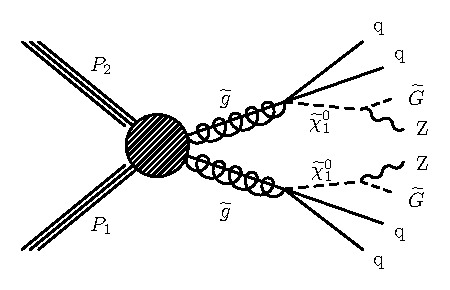
\includegraphics[width=\textwidth]{figures/diagrams/T5ZZ.pdf} 
        \caption{Strong GMSB SUSY}
        \label{fig:t5zz_diagram_interpretations}
      \end{subfigure}
      \begin{subfigure}[b]{0.49\textwidth}
        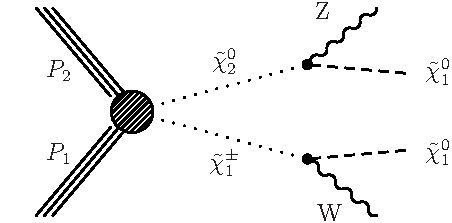
\includegraphics[width=\textwidth]{figures/diagrams/TChiWZ.pdf}
        \caption{EWK SUSY With WZ Production}
        \label{fig:tchiwz_diagram_interpretations}
      \end{subfigure} \\
      \begin{subfigure}[b]{0.49\textwidth}
        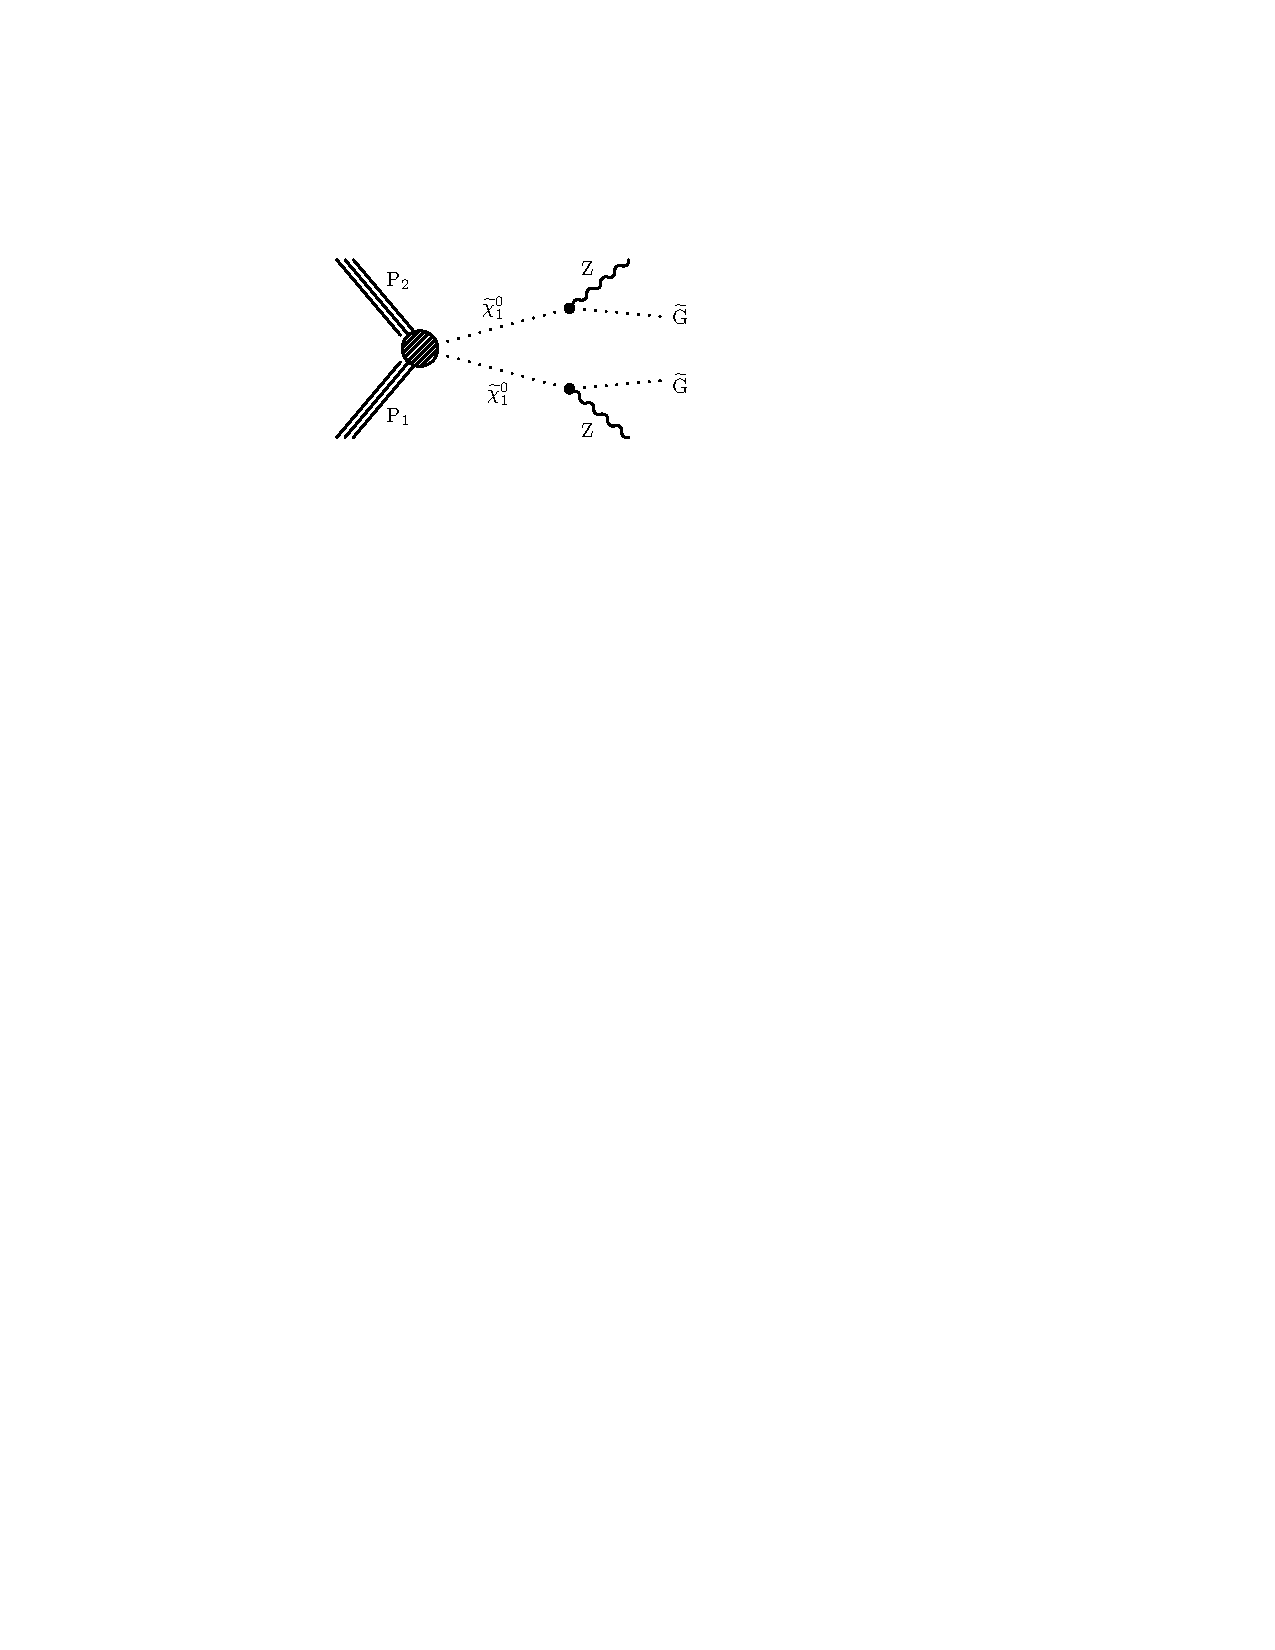
\includegraphics[width=\textwidth]{figures/diagrams/TChiZZ.pdf}
        \caption{EWK SUSY With ZZ Production}
        \label{fig:tchizz_diagram_interpretations}
      \end{subfigure}
      \begin{subfigure}[b]{0.49\textwidth}
        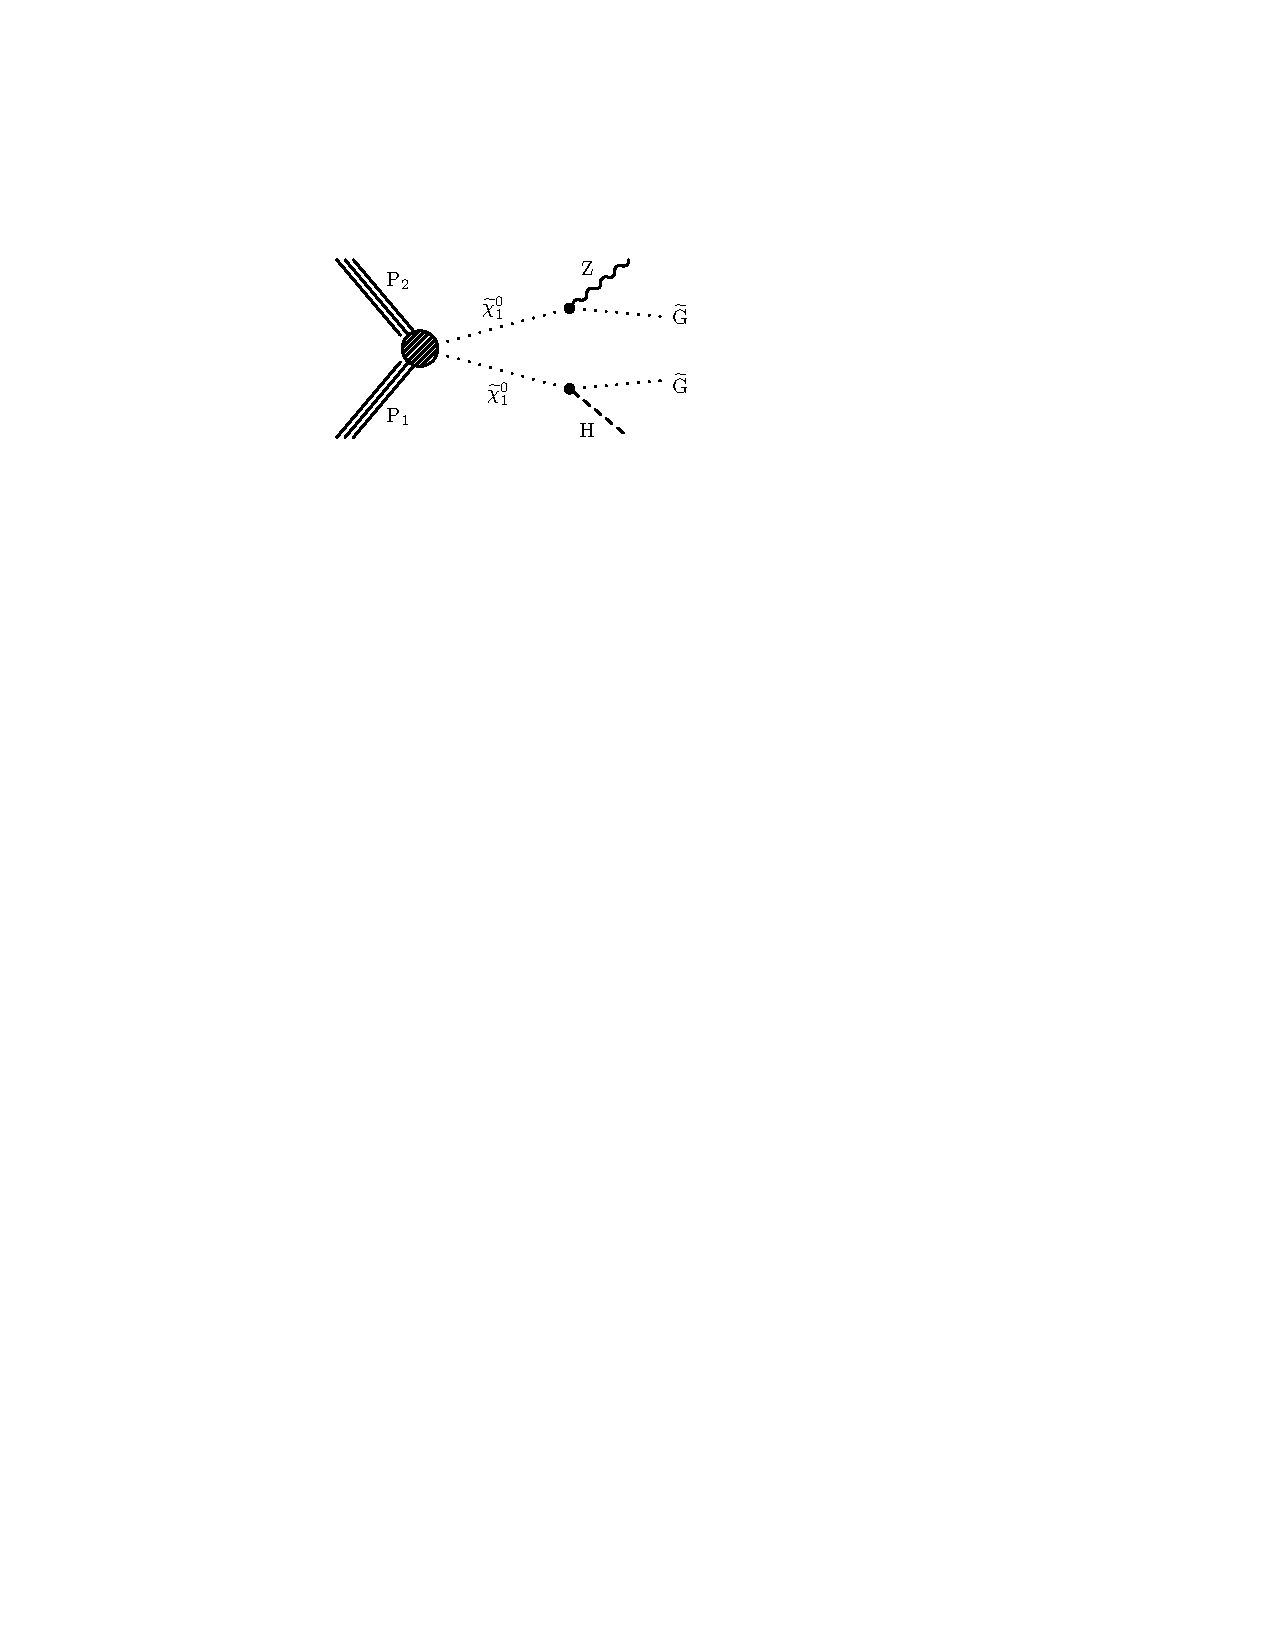
\includegraphics[width=\textwidth]{figures/diagrams/TChiHZ.pdf}
        \caption{EWK SUSY With HZ Production}
        \label{fig:tchihz_diagram_interpretations}
      \end{subfigure}
      \caption{ \label{fig:SUSY_diagrams_interpretation_sec}
        Feynman diagrams for the SUSY models used in interpreting the results of this analysis. More exposition on the properties of these models is found in sec \ref{sec:susy_models}.}
    \end{figure}

    For the strong production model, shown in fig. \ref{fig:t5zz_diagram_interpretations}, the exclusion limits are shown in figure \ref{fig:t5zz_interpretation}, which combines data from all the strong search regions in the likelihood function. The free parameters in this model are the gluino and $\widetilde{\chi}^0_1$ masses, the gravitino mass is set to 1 GeV. The bulk of the sensitivity comes from the high jet multiplicity and high \MET search regions, SRB(b) and SRC(b). Due to the downward fluctuations in most of the high \MET bins, our observed limit is slightly better than the expected limit. In a previous CMS result probing similar final states,\cite{paper_2015} this simplified model was excluded at the 95\% CL for gluino masses roughly below 1.2-1.3 TeV for $\widetilde{\chi}^0_1$ masses below 1 TeV. This analysis advances the limits significantly, by roughly 400 GeV in gluino mass for similar $\widetilde{\chi}^0_1$ masses, as can be seen in figure \ref{fig:t5zz_interpretation}. 

    \todo{check this description: }In the compressed spectrum (where the $\widetilde{\chi}^0_1$ mass is close to the gluino mass), the neutralino is expected to carry away more energy from the gluino than the quarks. In the extremely compressed regions where the $\widetilde{\chi}^0_1$ and gluino masses are only separated by about 100 GeV, it's possible that one of the jets can be missed. This makes SRB/SRBb more important regions at the top of the plot. The data shows a downward fluctuation in the high \MET bins of those regions, and so the observed limits tend to move towards higher masses than the expected limits. At large mass splittings, i.e. points near the x axis, SRC and SRCb are the most important regions due to the high jet multiplicity. There is a small upwards fluctuation in SRCb which offsets the downward fluctuations in SRB, SRBb, and SRC; this causes the observed limit to be closer to the expected limit in the bottom of the plot.

    \begin{figure}[!h]
      \centering
        \begin{subfigure}[b]{0.4\textwidth}
          \label{fig:t5zz_interpretations_2015}
          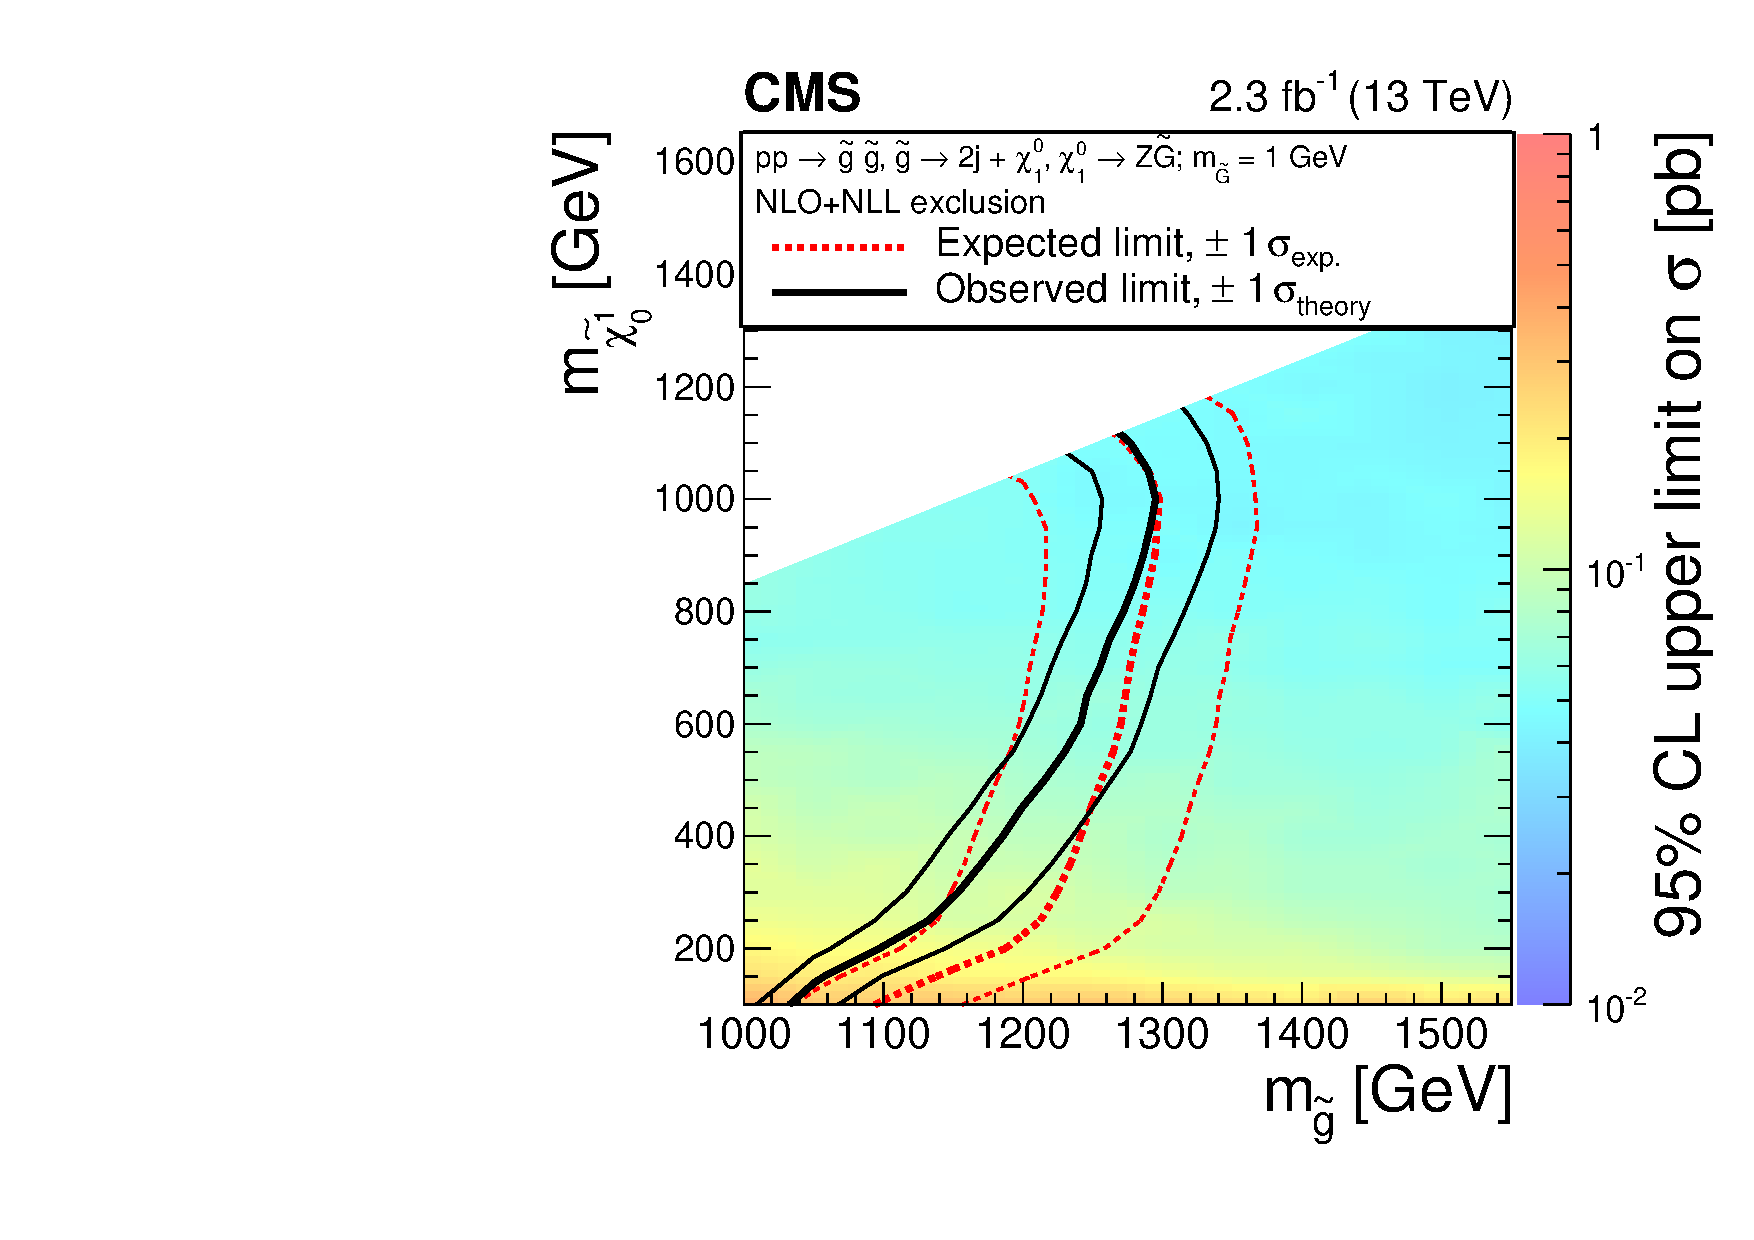
\includegraphics[width=\textwidth]{figures/interpretations/t5zz_2015_exclusion.pdf}
          \caption{Previous best limits on this model}
        \end{subfigure}
        \begin{subfigure}[b]{0.4\textwidth}
          \label{fig:t5zz_interpretations_current}
          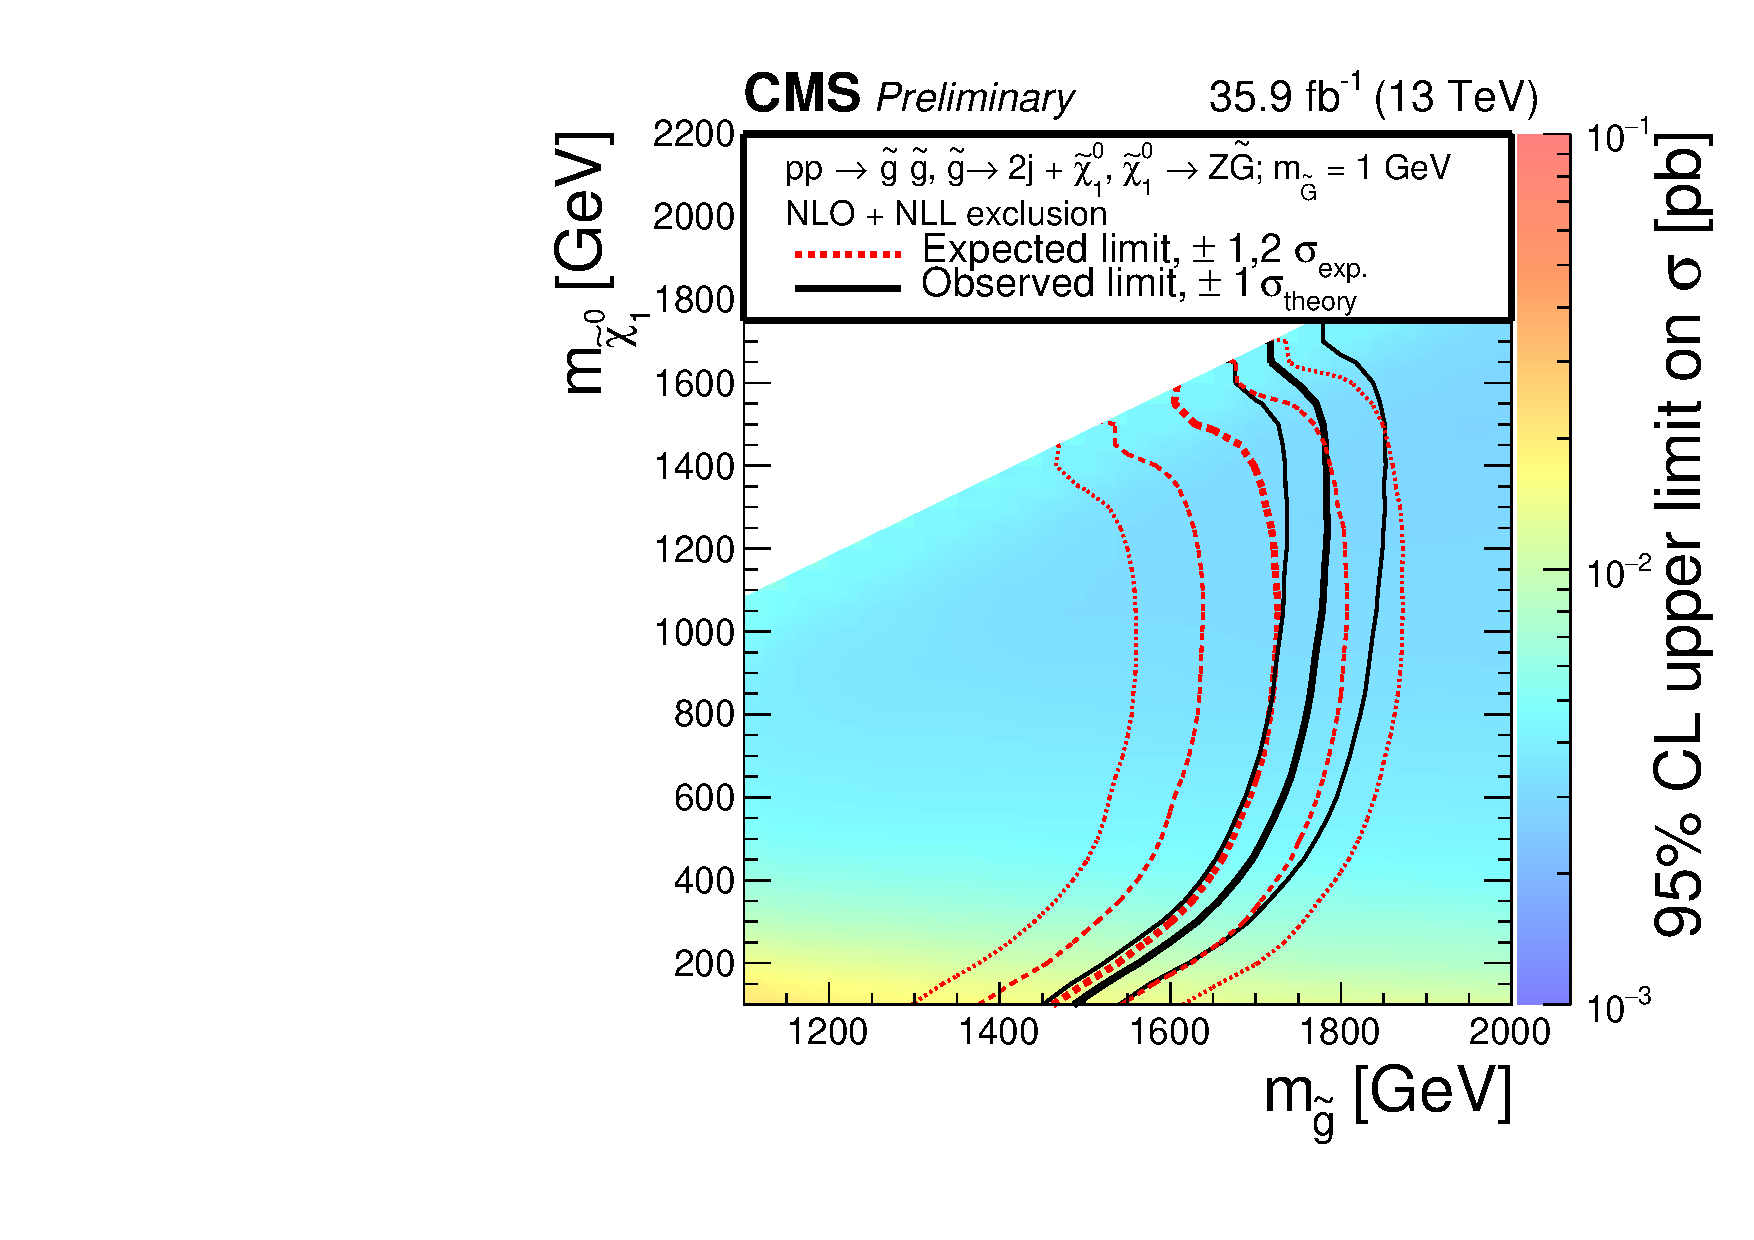
\includegraphics[width=\textwidth]{figures/interpretations/T5ZZ_Exclusion_13TeV.pdf}
          \caption{Limits set by this analysis}
        \end{subfigure}
      \caption{ \label{fig:t5zz_interpretation}
        The limits set on the strong GMSB SUSY model from fig. \ref{fig:t5zz_diagram_interpretations} are shown to the right. To the left, we show the previous best limit on this model set by CMS in 2016.\cite{paper_2015} The solid black and bold dotted red lines trace out the largest masses where the signal strength $\mu$ is less than 1 at 95\% confidence for observed and expected data respectively as described in section \ref{sec:setting_exclusion_limits}, mass points to the left of these line are excluded. The data excludes this model at the 95\% CL for gluino masses below 1450 GeV for low LSP masses, and below 1750 GeV for large LSP masses.
      }
    \end{figure}

    Figure \ref{fig:tchiwz_interpretation} shows the exclusion limits for the electroweak WZ model in fig. \ref{fig:tchiwz_diagram_interpretations}. For this model, data from the electroweak regions are used in the likelihood, however almost all the discriminatory power comes from the VZ region. The free parameters in this model are the mass of the $\widetilde{\chi}^0_1$ and $\widetilde{\chi}^{\pm}_1$, the $\widetilde{\chi}^0_2$ mass is set equal to that of the $\widetilde{\chi}^{\pm}_1$. Downward fluctuations in the high \MET bins for that region again make the observed limits stronger than the expected limits. For light LSP mass points, the model is excluded for $\widetilde{\chi}^{\pm}_1$ and $\widetilde{\chi}^0_2$ masses up to 600 GeV, better than double the previous limits. In the high $\widetilde{\chi}^{\pm}_1$ and $\widetilde{\chi}^0_2$ mass range, the excluded LSP mass range extends to around 250 GeV. 

    \begin{figure}[!h]
      \centering
        \begin{subfigure}[b]{0.4\textwidth}
          \label{fig:t5zz_interpretations_2015}
          \includegraphics[width=\textwidth]{figures/interpretations/TChiWZ_previous_best.pdf}
          \caption{Previous best limits on this model}
        \end{subfigure}
        \begin{subfigure}[b]{0.4\textwidth}
          \label{fig:t5zz_interpretations_current}
          \includegraphics[width=\textwidth]{figures/interpretations/TChiWZ_Exclusion_13TeV.pdf}
          \caption{Limits set by this analysis}
        \end{subfigure}
      \caption{ \label{fig:tchiwz_interpretation}
        The limits set on the electroweak WZ model in fig. \ref{fig:tchiwz_diagram_interpretations}. In this limit, data from the electroweak VZ and HZ search regions are utilized, though the VZ region has by far the larger sensitivity to this model. The solid back and thick dashed red lines show the observed and expected limits respectively as described in section \ref{sec:setting_exclusion_limits}, mass points below these lines are excluded. These results push the excluded $\widetilde{\chi}^{\pm}_1$ and $\widetilde{\chi}^0_2$ masses to 600 GeV from 275 GeV for low mass LSPs, and excludes LSP mass points for up to about 250 GeV for high $\widetilde{\chi}^{\pm}_1$ and $\widetilde{\chi}^0_2$ masses, up from about 60.
      }
    \end{figure}

    Figure \ref{fig:tchizz_interpretation}, shows the exclusion limits for the electroweak ZZ model shown in fig. \ref{fig:tchizz_diagram_interpretations}. In this model, the only free parameter is the mass of the $\widetilde{\chi}^0_1$, the gravitino mass is assumed to be 1 GeV. The thick pink line is the theoretical cross section for this model as a function of the free mass parameter, it's thickness shows the uncertainty on the theory calculation. The solid black and dotted black lines show the observed and expected limits respectively. The point where the pink line and the solid black line cross is the observed exclusion limit for the $\widetilde{\chi}^0_1$ mass at 95\% confidence. This result pushed the previous limits on the $\widetilde{\chi}^0_1$ mass from about 375 GeV to about 675 GeV.


    \begin{figure}[!h]
      \centering
        \begin{subfigure}[b]{0.4\textwidth}
          \label{fig:t5zz_interpretations_2015}
          \includegraphics[width=\textwidth]{figures/interpretations/TChiZZ_previous_best.pdf}
          \caption{Previous best limits on this model}
        \end{subfigure}
        \begin{subfigure}[b]{0.4\textwidth}
          \label{fig:t5zz_interpretations_current}
          \includegraphics[width=\textwidth]{figures/interpretations/TChiZZ_Exclusion_13TeV.pdf}
          \caption{Limits set by this analysis}
        \end{subfigure}
      \caption{ \label{fig:tchizz_interpretation}
        The limits set on the Electroweak ZZ model shown in fig. \ref{fig:tchizz_diagram_interpretations}. In this limit, data from the electroweak VZ search region is utilized and the $\widetilde{\chi}^0_1$ is assumed to decay 100\% to the Z. On the right, the point where the pink line crosses the solid black line marks the highest mass excluded. Where the pink line crosses the dotted line marks the expected limit. The downward fluctuation in the VZ region high \MET bin again caused the observed limit to be better than the expected limit. The limit set on the $\widetilde{\chi}^0_1$ mass increased by about 300 GeV from the previous result on the left.
      }
    \end{figure}

    Finally, figure \ref{fig:tchihz_interpretation}, shows the exclusion limits for the electroweak HZ model shown in fig. \ref{fig:tchihz_diagram_interpretations}. The only free parameter in this model is the $\widetilde{\chi}^0_1$ mass. This model assumes a 50\% branching ratio of the $\widetilde{\chi}^0_1$ to higgs and Z bosons. The likelihood for this model is constructed using data from the VZ and HZ regions. The likelihood also takes into account that the signature of the ZZ model above should be produced with $\frac{1}{2}$ the frequency as that of the HZ model since the 50\% branching ratio to Z bosons means that the ZZ final state should be produced as well. Points to the left of the crossing point between the pink and solid black line are excluded at the 95\% level. This analysis pushed the limits for the $\widetilde{\chi}^0_1$ mass in this model from 250 GeV to about 500 GeV.

    \begin{figure}[!h]
      \centering
        \begin{subfigure}[b]{0.4\textwidth}
          \label{fig:t5zz_interpretations_2015}
          \includegraphics[width=\textwidth]{figures/interpretations/TChiHZ_previous_best.pdf}
          \caption{Previous best limits on this model}
        \end{subfigure}
        \begin{subfigure}[b]{0.4\textwidth}
          \label{fig:t5zz_interpretations_current}
          \includegraphics[width=\textwidth]{figures/interpretations/TChiHZ_0p25ZZ_Exclusion_13TeV.pdf}
          \caption{Limits set by this analysis}
        \end{subfigure}
      \caption{ \label{fig:tchihz_interpretation}
        The limits set on the Electroweak HZ model shown in fig. \ref{fig:tchihz_diagram_interpretations}. In this limit, data from the electroweak VZ and HZ search regions are combined and the branching ratios for $\widetilde{\chi}^0_1$ are assumed to be 50/50 between the Higgs and Z.
      }
    \end{figure}

  \clearpage

\section{The Electroweak Combination}

The things we want to consider here are: 

  1. All the cuts and stuff, I want to list out what cuts we made and why we chose them. I am not sure where I will put all the data/MC agreement stuff. I guess that's mostly important for the MET profile as I don't really use MC in the rest of the

  \chapter{Conclusions}

\section{What the hell did I do, and what didn't I do?}

\begin{itemize}
  \item I executed all the work to get the data from the babies and put them into histograms
  \item I implemented all the signal regions in code
  \item I implemented all the background methods in code, including the MET templates and the FS BG with the RSFOF transfer factor
  \item MET Templates closure test, deriving the error bars there 
  \item I made all the plots and tables we used EXCEPT the temperature plots
  \item I ran everything through combine
  \item I found all the uncertainty ranges by running everything through with varied quantities
\end{itemize}

\begin{itemize}
  \item I did not make the temperature plots for the interpretations, but did provide the histograms for them
  \item I did not make the covariance matricies
  \item I did not measure any of the uncertainty sources (i.e. I used the Btag working groups scale factors, I didn't measure the lepton trigger efficiencies or ID/ISO efficiencies).
  \item I did basically no writing of the AN or the paper.
\end{itemize}

  \chapter{Glossary Of Terms} \label{ch:glossary}

\begin{itemize}
\item{$H_T$} The scalar sum of the momentum in the transverse plane over all jets in an event. If there are two jets pointing at arbitrary angles with total energy $E_a=\sqrt{p_{a,x}^2 + p_{a,y}^2}$ and $E_b=\sqrt{p_{b,x}^2 + p_{b,y}^2}$ respectively, the $H_T$ for that event would be simply $E_a + E_B$

\item{ISR/FSR} Initial and Final State Radiation

\item{Light lepton} An electron or muon or their antiparticle partners.

\item{OCSF} Opposite charge, same flavor. Used in the context of events with two light leptons, meaning either $e^+e^-$ or $\mu^+ \mu^-$.

\item{OCDF} Opposite charge, different flavor. Used in the context of events with two light leptons, meaning either $e^+\mu^-$ or $\mu^+ e^-$.

\item{prompt} A particle is called prompt if it was generated at the primary interaction vertex. A particle is called non-prompt if it was created in the decay of another particle further down the decay chain. 

\item{FromPV} From: https://twiki.cern.ch/twiki/bin/view/CMSPublic/WorkBookMiniAOD2015 The meaning of fromPV() results are unchanged, fromPV() returns a number between 3 and 0 to define how tight the association with the PV is: 
the tighest, 3 (PVUsedInFit), is if the track is used in the PV fit;
2 (PVTight) is if the track is not used in the fit of any of the other PVs, and is closest in z to the PV,
1 (PVLoose) is if the track is closest in z to a PV other then the PV.
0 (NoPV) is returned if the track is used in the fit of another PV.

\item{PVTight} See FromPV

\item{$M_T$} Transverse Mass, the mass of a 4 vector with the z-component set to 0.

\end{itemize}



  %% END MATTER
  % \printindex %% Uncomment to display the index
  % \nocite{}  %% Put any references that you want to include in the bib 
  %               but haven't cited in the braces.
  \bibliographystyle{plain}  %% This is just my personal favorite style. 
  %                              There are many others.
  %\setlength{\bibleftmargin}{0.25in}  % indent each item
  %\setlength{\bibindent}{-\bibleftmargin}  % unindent the first line
  %\def\baselinestretch{1.0}  % force single spacing
  %\setlength{\bibitemsep}{0.16in}  % add extra space between items
  \bibliography{template}  %% This looks for the bibliography in template.bib 
  %                          which should be formatted as a bibtex file.
  %                          and needs to be separately compiled into a bbl file.
\end{document}

